\documentclass{article}
\usepackage{multirow}
\usepackage{graphicx}
\usepackage{booktabs}
\usepackage{enumitem}
\usepackage{siunitx}
\usepackage{optidef}
\usepackage{booktabs}
\usepackage{caption}   % for \captionof
\usepackage{xcolor}
\usepackage{xurl}
\usepackage{amsmath}
\DeclareMathOperator*{\minimize}{minimize}
 \usepackage[final,main]{neurips_2026}
\usepackage[breakable]{tcolorbox}
\usepackage[utf8]{inputenc} % allow utf-8 input
\usepackage[T1]{fontenc}    % use 8-bit T1 fonts
\usepackage{hyperref}       % hyperlinks
\hypersetup{colorlinks=true, linkcolor=blue, citecolor=blue, urlcolor=blue}
\usepackage{url}            % simple URL typesetting
\usepackage{titletoc}       % appendix-only local table of contents (Hawkeye-style)
\dottedcontents{section}[1.6em]{\bfseries}{1.6em}{0.7pc}
\dottedcontents{subsection}[4.0em]{}{2.4em}{0.7pc}
\dottedcontents{subsubsection}[6.8em]{}{3.2em}{0.7pc}
\usepackage{booktabs}       % professional-quality tables
\usepackage{amsfonts}       % blackboard math symbols
\usepackage{amsmath}
\usepackage{amssymb}
\usepackage{nicefrac}       % compact symbols for 1/2, etc.
\usepackage{microtype}      % microtypography
\usepackage{xcolor}         % colors
\usepackage{graphicx}
\usepackage{algorithm}
\usepackage{stmaryrd}
\usepackage{fontenc}
\usepackage{enumitem}
\usepackage{algorithmic}
\definecolor{grey}{gray}{0.5}
\usepackage{multirow}
\usepackage{array}
\usepackage{amsthm}
\usepackage[capitalise]{cleveref}  % must come after hyperref
\usepackage{wrapfig}
\usepackage{tikz}
\usepackage{colortbl}
\usetikzlibrary{arrows.meta,positioning,fit,backgrounds}
\newtheorem{proposition}{Proposition}
\definecolor{skyblue}{RGB}{65, 155, 225}

\usepackage[T1]{fontenc}
\usepackage[utf8]{inputenc}
\usepackage{amsmath, amssymb}
\usepackage{booktabs}
\usepackage{tabularx}
\usepackage{array}
\usepackage{enumitem}
\usepackage{microtype}
\usepackage{pdflscape}
\theoremstyle{plain}
\newtheorem{theorem}{Theorem}
\newtheorem{corollary}{Corollary}
\newtheorem{definition}{Definition}
\theoremstyle{remark}
\newtheorem*{remark}{Remark}


\newcommand{\mnote}[1]{}
\renewcommand{\mnote}[1]{\textcolor{blue}{\textbf{[NOTE: #1]}}}

\newcommand{\ie}{\textit{i.e.}}
\newcommand{\eg}{\textit{e.g.}}
\newcommand{\acroletter}[1]{\textbf{\textsc{#1}}}
\newcommand{\etal}{\textit{et al.}}
\newcommand{\todo}[1]{\textcolor{red}{\textbf{[TODO: #1]}}}
\newcommand{\Tmax}{T^{\max}}
\newcommand{\Tmin}{T^{\min}}
\newcommand{\CGM}{C_{\text{GM}}}


\DeclareMathOperator*{\argmin}{arg\,min}


\title{Accelerating the Inference Era with AI-Driven, Globally Optimized HW/SW Co-Design}

\author{%
    Miria Feng \\
    Electrical Engineering \\
    Stanford University \\
    \texttt{miria0@stanford.edu}
    \And
    Fangzhao Zhang \\
    Electrical Engineering \\
    Stanford University \\
    \texttt{zfzhao@stanford.edu} 
    \And
    Adrian Lafuente \\
    Computer Science \\
    Stanford University \\
    \texttt{agamarra@stanford.edu}
    \And
    Mert Pilanci \\
    Electrical Engineering \\
    Stanford University \\
    \texttt{pilanci@stanford.edu}
    \And
    Azalia Mirhoseini \\
    Computer Science \\
    Stanford University \\
    \texttt{azalia@stanford.edu}
}



\begin{document}

\maketitle


\begin{abstract}
Deep learning inference demand is projected to grow $10{,}000\times$ over the next five years, a trajectory general-purpose accelerators cannot match. Custom inference accelerators offer a viable path forward, but designing them requires coordinating hardware datapaths, software schedules, and compiler transformations across a combinatorial design space exceeding $\mathcal O(10^{2300})$. Sequential pipelines discard alternatives before their global memory consequences are known. We introduce \textsc{CHEETAH}, an AI-guided co-design framework built around one master LP relaxation. Time-indexed placement and rematerialization expose reuse across operations and decode steps; McCormick envelopes couple tiling with fusion; and shared hardware variables jointly allocate compute, capacity, and bandwidth under area and power budgets. Disaggregated epigraphs and implementation menus represent competing service costs and discrete design choices. The operator-based GPU solver OCS optimizes working programs without forming the complete temporal matrix. An LLM architect proposes interventions using resource prices and trial diagnostics; integral recovery and replay establish feasible designs separately from relaxation bounds. Across eleven original workloads, CHEETAH achieves an average predicted $22.07\times$ speedup and up to $40.1\times$ over modeled TPU-v3 within six hours of search. A full-inference DeepSeek-V3 design predicts $22.88\times$ overall, $13.39\times$ prefill, and $28.20\times$ decode acceleration under a declared memory-interface model. Matched controls isolate batching, fusion, KV retention, and temporal placement gains.
\end{abstract}



\section{Introduction}
\label{sec:introduction}
AI inference demand is expected to grow by $10{,}000\times$ over the next five
years~\citep{cra2026aifuture}. General-purpose accelerators leave significant
efficiency gains unrealized, which motivates accelerators specialized to their
target workloads. Specialization, however, requires coordinating datapaths,
memory capacity, mappings, and compiler transformations, and the resulting
design space can exceed $\mathcal O(10^{2300})$~\citep{zhang_fast}. Engineers typically explore it in
stages: choose hardware, map each operation, then optimize data reuse. Automation
accelerates these stages without necessarily removing their information loss.
A locally faster tile can consume the memory needed to retain a neighboring
tensor; a slightly slower tile can therefore yield a faster complete schedule.

We introduce \textsc{CHEETAH}: \acroletter{C}o-designed \acroletter{H}ardware
\acroletter{E}xploration via \acroletter{E}fficient \acroletter{T}hroughput and
\acroletter{H}ybrid-search. One master LP relaxation exposes these interactions
jointly. Its implementation choices determine work, traffic, and workspace;
time-indexed states track residency and reuse; and shared hardware variables
allocate compute, vector, memory, and bandwidth resources under area and power
budgets. McCormick envelopes and disaggregated epigraphs keep the model linear.
The relaxation supplies bounds for its declared domain, while integral recovery
and replay supply a concrete chip and software schedule. These are distinct
outputs: a low fractional objective alone is not an executable design.

\paragraph{One program, many architectures.}
The formulation operates on a graph of independent logical invocations and
typed storage objects. Convolutions, dense and expert GEMMs, attention, and
vector operations contribute implementation-specific coefficients and
dependencies. Optional batches and fusion groups cover original invocations
without erasing their identities. KV prefixes, expert weights, and long skip
connections enter the same capacity and readiness accounting. This makes the
program reusable across architectures without assuming that identical shapes
must share a decision.

\paragraph{Beyond prefill: the decode memory wall.}
Prefill amortizes weight traffic across many tokens; autoregressive decode
repeatedly accesses weights and an expanding KV history. Batching helps, but
sparse routing also increases the number of experts touched. Under independent
uniform top-$k$ routing, the expected union is
$n[1-(1-k/n)^B]$: with $n=256$, $k=8$, it grows from $8$ experts at batch one
to about $163$ at batch $32$. Thus batching does not guarantee a compute-bound
decode phase. CHEETAH jointly chooses resource provisioning, compatible
batches, and temporal residency. Our full-inference experiment uses actual
routes, retains the complete KV history, and charges every restore; its gains
do not assume that all weights or KV fit on chip.

\paragraph{Scaling the search.}
The complete temporal program is too large to materialize. OCS evaluates linear
operators and adjoints on compact working supports, using GPU first-order
updates, reversible scaling, and structured temporal incidence. Full-domain
checking remains separate from a working solve. An LLM architect reads resource
prices and trial diagnostics to propose implementations or search neighborhoods;
deterministic checks decide whether to admit them. The original campaign couples
this controller to Vizier; the master also admits hardware choices directly.

\paragraph{Contributions.}
\begin{enumerate}[leftmargin=*,itemsep=2pt,topsep=3pt]
\item A unified LP abstraction for hardware sizing, joint tiling--fusion,
time-indexed placement, and rematerialization, with explicit causal storage and
service constraints for full inference.
\item An operator-based solution path combining OCS, compact temporal
representations, checked bounds, and independently replayed integral recovery.
\item A diagnostic-guided LLM architect that reduces invalid trials in the
original campaign from $24.5\%$ to $5.9\%$ without replacing feasibility checks.
\item Predicted accelerator gains across vision, language, and diffusion
workloads, plus a full-input DeepSeek design with $22.88\times$ overall speedup
and matched prefill/decode feature controls. RTL and synthesis studies test
selected mechanisms; the full-task latency remains an analytical prediction.
\end{enumerate}

Section~\ref{sec:related} positions the work; Section~\ref{sec:prelim}
explains sequential information loss and relaxation. Section~\ref{sec:methods}
presents the master and its feature encodings, and Section~\ref{sec:ocs} describes
OCS. Section~\ref{sec:experiments} reports the original campaign and the full-input
phase and feature results. The appendix provides complete rows, containment
arguments, physical-validation details, economics, and reproduction evidence.


% ---- plots restored from the long version, original placement ----

\begin{figure}[ht!]
    \centering
    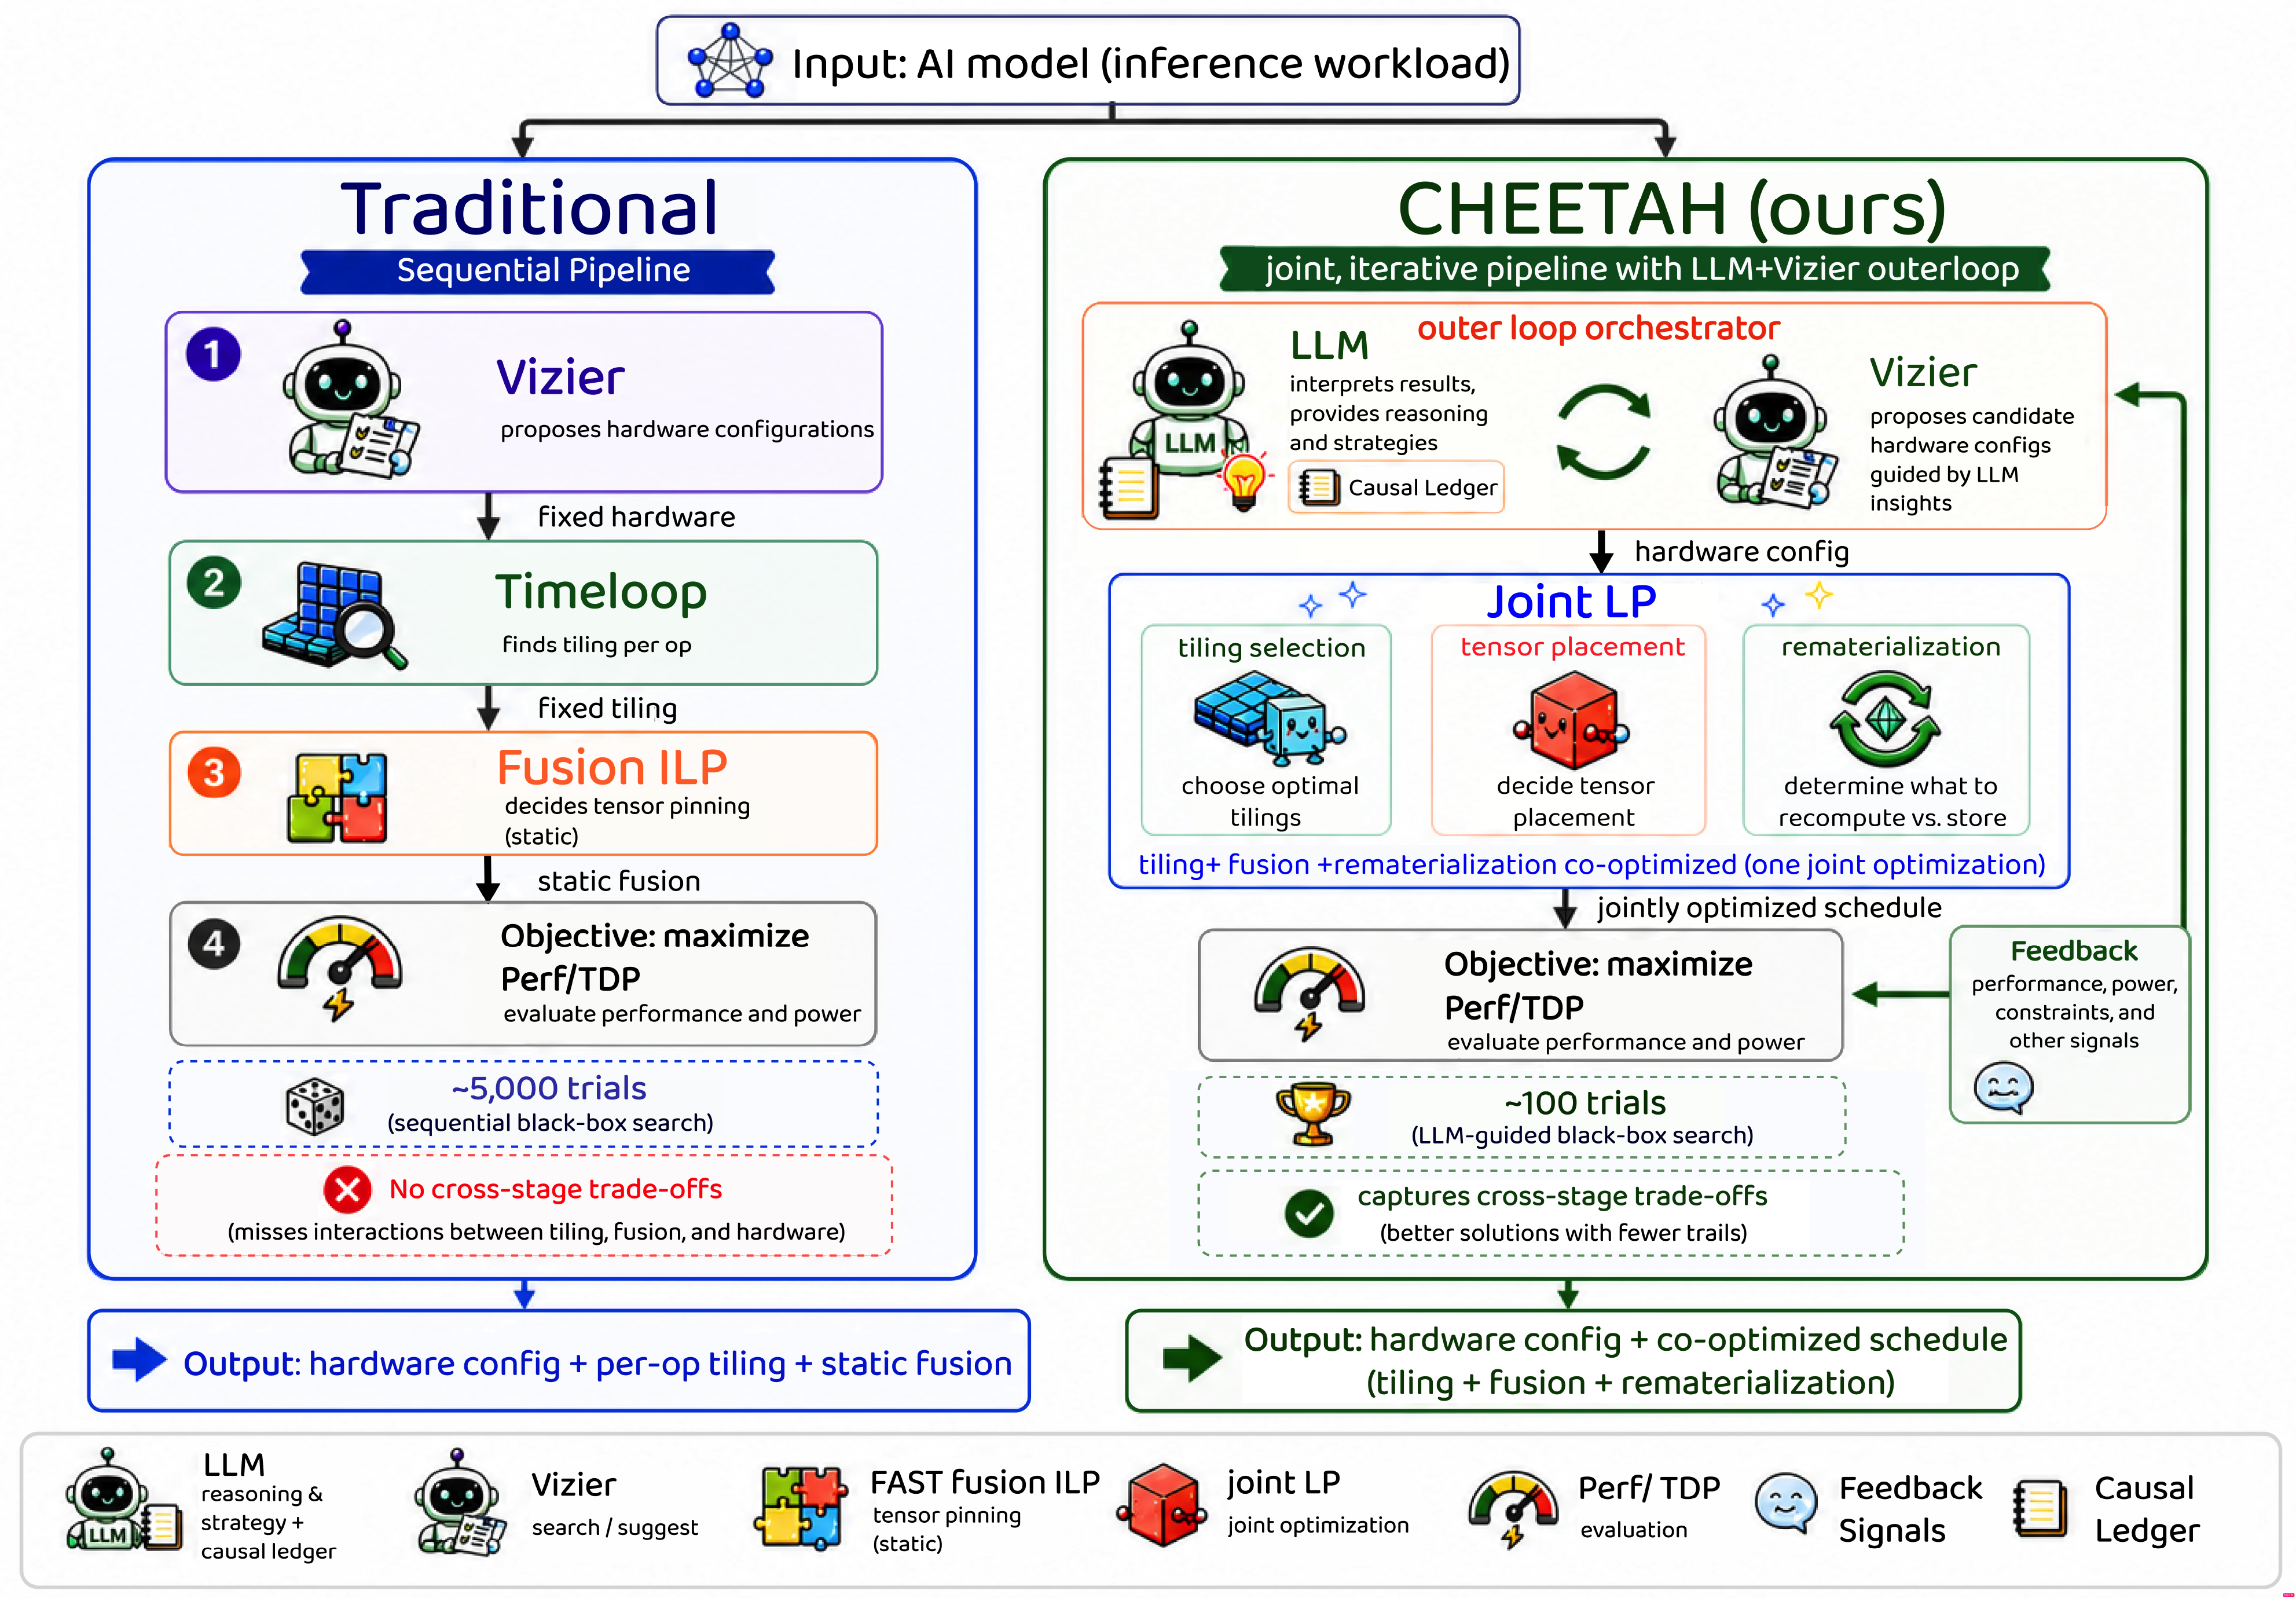
\includegraphics[width=1.0\linewidth]{figs/cheetah_v4_new.png}
\caption{Sequential vs Our Unified Optimization Paradigm.
(Left) Baseline methods decouple hardware search, operation-level tiling, and static fusion; precluding cross-stage trade-offs.
(Right) CHEETAH presents a unified LLM-driven LP-solver-based framework that jointly optimizes tiling, placement, and rematerialization while learning from a causal ledger.}
\label{fig::workflow}
\end{figure}

\begin{figure}[ht!]
    \centering
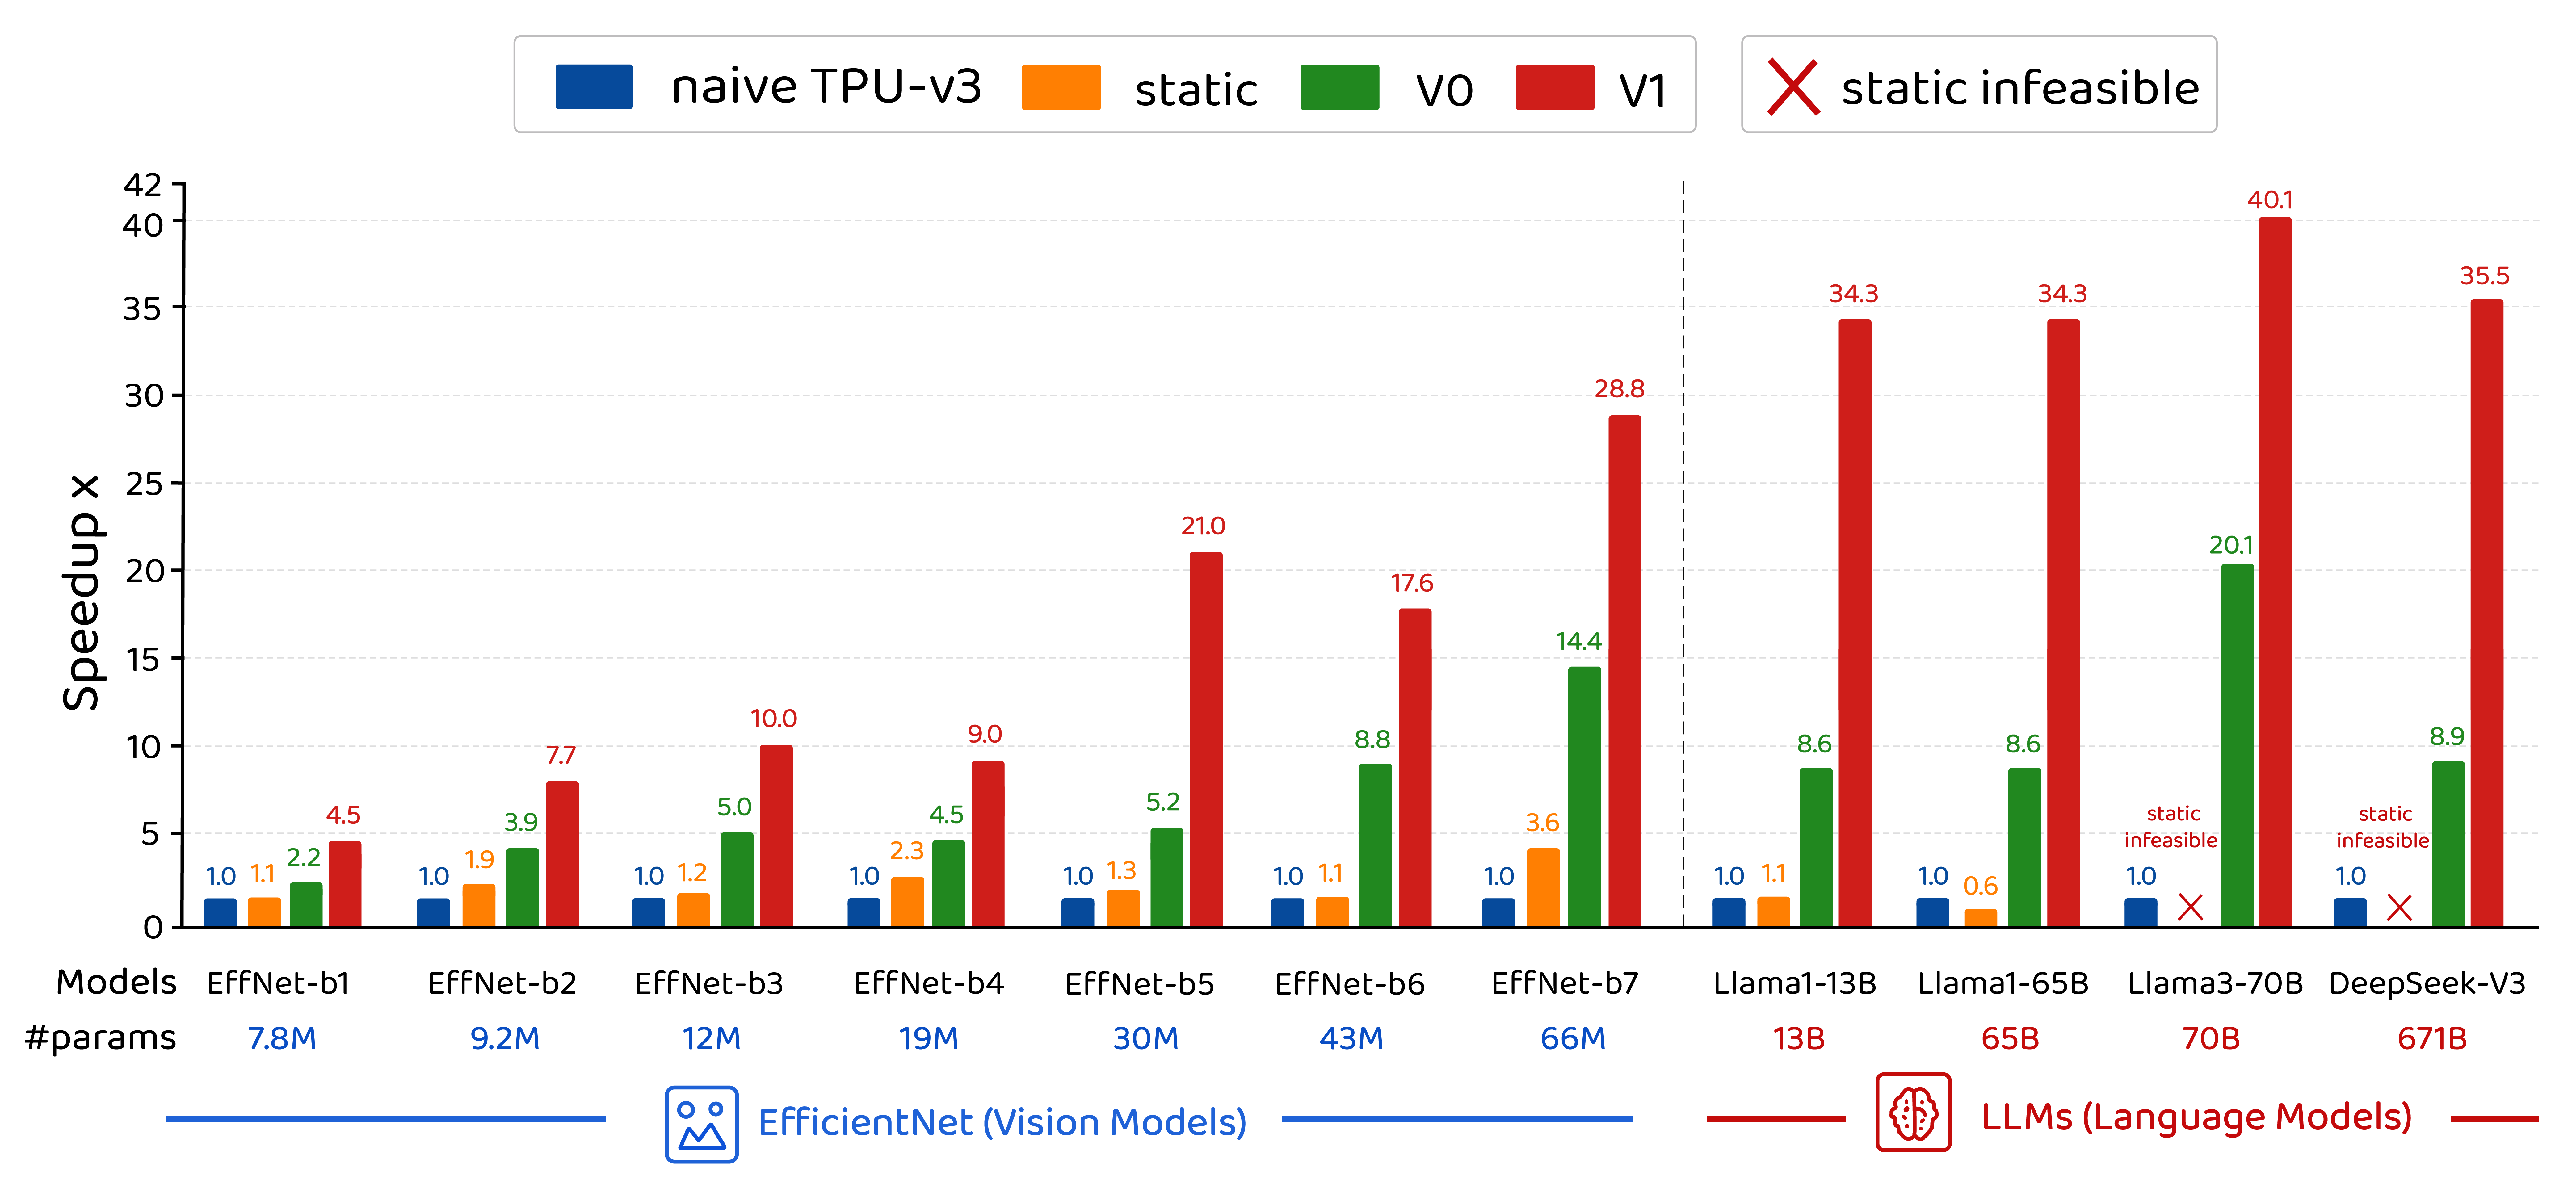
\includegraphics[width=1.0\linewidth]{fig3/speedup_final_v3.png}
\caption{Speedup over modeled TPU-v3 baseline for each workload and formulation: CHEETAH-V1's joint tiling-fusion optimization achieves up to $\sim$40.1$\times$ acceleration, while static fusion is infeasible on large-scale LLMs. Progressive gains are visible across formulations: V0's dynamic placement improves over static by $2$--$20\times$, while V1's joint tiling-fusion adds another $2$--$4\times$ on top. See Section~\ref{sec:experiments} for full analysis and wall-clock time breakdowns.}
\label{fig:speedup}
\end{figure}

\section{Related Work}
\label{sec:related}
Accelerator mappers such as Timeloop, CoSA, and ZigZag explore tiling and
mapping; FAST connects hardware search, mapping, and fusion in a staged
flow~\citep{timeloop,huang2021cosaschedulingconstrainedoptimization,mei2021zigzag,zhang_fast}.
DOSA jointly differentiates hardware and mapping choices, while Gemini explores
chiplet architectures and layer pipelines~\citep{hong2023dosa,cai2024gemini}.
TileFlow and FADiff address fusion-aware dataflows and joint mapping--fusion
optimization~\citep{zheng2023tileflow,jia2025fadifffusionawaredifferentiableoptimization}.
CHEETAH couples these choices to temporal storage and shared hardware in an LP
relaxation; this is a distinction in formulation, not a claim that prior work
lacks joint optimization altogether.

\paragraph{Capability comparison table.}
Table~\ref{tab:capability-matrix} distinguishes searched decisions from restricted
or user-specified support. DeFiNES chooses caching versus overlap recomputation,
Fast-and-Fusiest searches dependency-respecting orders within its fused mapspace.
Gemini's fusion and order support concerns layer pipelines. Pluto optimizes
affine schedules, Tiramisu also exposes explicit storage, copies, and redundant
computation through its scheduling language. These differ from unrestricted
cost-driven temporal placement. CoSA's guarantee concerns a per-layer proxy
objective, and Fast-and-Fusiest's concerns its fixed-hardware mapspace, but neither
is a bound over a joint hardware--schedule domain. The last column denotes one joint mathematical program, rather than staged
co-search. DOSA's qualifying program is nonconvex.

First-order solver methods~\citep{applegate2022practicallargescalelinearprogramming}
and McCormick envelopes~\citep{mccormick1976computability} supply the optimization
building blocks. LLM proposal systems such as FunSearch and
AlphaEvolve~\citep{romera2024mathematical,novikov2025alphaevolvecodingagentscientific}
inform the outer-loop role: propose changes, then evaluate them independently.
Further comparisons appear in Appendix~\ref{related_work_appendix}.


\section{Preliminaries}\label{sec:prelim}
\subsection{Sequential Design and Information Loss}
\label{sec:background_pipeline}
Accelerator design commonly proceeds from a resource budget to a hardware
template, then to operation mappings and a memory schedule. Engineers iterate
these choices using analytical models, simulation, and compiler feedback.
Automated flows replace individual choices with search tools, but an early
commitment still limits what downstream stages can recover. A mapper that
exports only its fastest isolated tile discards alternatives that might reduce
workspace, enable fusion, or retain data for a later consumer. Joint design
keeps those alternatives available until their complete resource costs are known.

\subsection{Linear Relaxation and Recovery}
\label{sec:lps}
An LP minimizes a linear objective subject to linear rows and coordinate
bounds. Discrete implementation selections are relaxed to $[0,1]$; bounded
products are represented by convex envelopes. The resulting optimum is a
lower bound only for the domain actually covered by the formulation and its
certificate. Fractional selections need not describe a chip. Recovery chooses
integral hardware and implementations, then checks dependencies, storage,
transfers, and predicted latency. A feasible recovered design is useful even
when the remaining optimality interval is wide.

\subsection{Capability Comparison}
\label{sec:capability-matrix}
Table~\ref{tab:capability-matrix} compares decision spaces, rather than claiming
that every listed capability has a measured gain. CHEETAH's row describes the
master formulation; Section~\ref{sec:decode_decomp} identifies the subset exercised
by the current full-inference execution. Related Work explains restricted cells.

% Table 1: decision spaces in the cited systems.
% Visual restored to the earlier colored design (green/red/amber marks,
% banded column groups, alternating row shading, family grouping rows).
% Citations stay in the System column, not in the caption.
\definecolor{cmgood}{RGB}{20,120,50}
\definecolor{cmbad}{RGB}{190,40,40}
\definecolor{cmpart}{RGB}{200,130,0}
\providecommand{\cmark}{\textcolor{cmgood}{\ensuremath{\checkmark}}}   % searched/formulated
\providecommand{\xmark}{\textcolor{cmbad}{\ensuremath{\times}}}        % not searched
\providecommand{\pmark}{\textcolor{cmpart}{\ensuremath{\circ}}}        % restricted/user-specified

\begin{table}[t]
\centering
\caption{Decision spaces in the cited systems. \cmark: formulated;
\pmark: restricted or user-specified; \xmark: not in the cited method.
Guarantees retain their own objective and domain. CHEETAH's row demonstrates our unified formulation scope.}
\label{tab:capability-matrix}
\scriptsize\setlength{\tabcolsep}{2.1pt}\renewcommand{\arraystretch}{1.18}
\definecolor{bandsched}{RGB}{230,239,253}
\definecolor{bandsearch}{RGB}{230,245,233}
\definecolor{bandguar}{RGB}{253,234,234}
\definecolor{rowalt}{gray}{0.955}
\definecolor{rowours}{gray}{0.875}
\providecommand{\hdr}[1]{\begin{tabular}[b]{@{}c@{}}#1\end{tabular}}
\providecommand{\famrow}[1]{\multicolumn{10}{@{}l}{\textit{#1}}}
\begin{tabularx}{\linewidth}{@{}Xccccccccc@{}}
\toprule
 & \multicolumn{5}{c}{\cellcolor{bandsched}\textbf{Schedule decisions}}
 & \multicolumn{2}{c}{\cellcolor{bandsearch}\textbf{Search}}
 & \multicolumn{2}{c}{\cellcolor{bandguar}\textbf{Guarantee}} \\
\cmidrule(lr){2-6}\cmidrule(lr){7-8}\cmidrule(lr){9-10}
\textbf{System} & \hdr{Per-op\\tiling} & Fusion & \hdr{Temporal\\placement} & Remat. &
\hdr{Op.\\order} & Mapping & \hdr{HW\\sizing} & \hdr{Opt.\\guarantee} & \hdr{Joint HW/SW\\program} \\
\midrule
\famrow{Per-op mappers} \\
Timeloop~\citep{timeloop} & \cmark & \xmark & \xmark & \xmark & \xmark & \cmark & \xmark & \xmark & \xmark \\
\rowcolor{rowalt}
CoSA~\citep{huang2021cosaschedulingconstrainedoptimization} & \cmark & \xmark & \xmark & \xmark & \xmark & \cmark & \xmark & \pmark & \xmark \\
\famrow{Fusion-aware mappers} \\
DeFiNES~\citep{mei2023defines} & \cmark & \cmark & \pmark & \pmark & \pmark & \cmark & \xmark & \xmark & \xmark \\
\rowcolor{rowalt}
Fast-and-Fusiest~\citep{andrulis2026fusiest} & \cmark & \cmark & \pmark & \xmark & \cmark & \cmark & \xmark & \pmark & \xmark \\
\famrow{Hardware design-space exploration} \\
ZigZag~\citep{mei2021zigzag} & \cmark & \xmark & \xmark & \xmark & \xmark & \cmark & \cmark & \xmark & \xmark \\
\rowcolor{rowalt}
DOSA~\citep{hong2023dosa} & \cmark & \xmark & \xmark & \xmark & \xmark & \cmark & \cmark & \xmark & \cmark \\
Gemini~\citep{cai2024gemini} & \cmark & \pmark & \pmark & \xmark & \pmark & \cmark & \cmark & \xmark & \xmark \\
\rowcolor{rowalt}
CODEBench~\citep{Tuli_2023} & \pmark & \xmark & \xmark & \xmark & \xmark & \xmark & \cmark & \xmark & \xmark \\
FAST~\citep{zhang_fast} & \cmark & \cmark & \pmark & \xmark & \xmark & \cmark & \cmark & \xmark & \xmark \\
\famrow{Loop compilers} \\
\rowcolor{rowalt}
Pluto~\citep{bondhugula2008pluto} & \pmark & \cmark & \xmark & \xmark & \cmark & \pmark & \xmark & \xmark & \xmark \\
Tiramisu~\citep{baghdadi2019tiramisu} & \pmark & \pmark & \pmark & \pmark & \pmark & \pmark & \xmark & \xmark & \xmark \\
\midrule
\rowcolor{rowours}
\textbf{CHEETAH (our framework)} & \cmark & \cmark & \cmark & \cmark & \cmark & \cmark & \cmark & \pmark & \cmark \\
\bottomrule
\end{tabularx}
\end{table}


\section{CHEETAH Formulation for HW/SW Co-Design}
\label{sec:methods}
CHEETAH minimizes input workload inference time under a declared pre-RTL hardware budget.
The input is a graph of logical invocations, a finite implementation library,
and a numerical contract. Hardware is shared across every invocation, operation
choices remain independent. The formulation includes the supplied schedule model and
causal execution alternatives as whole-program branches, preserving existing
feasible points while admitting richer implementations.

\subsection{Pruning, Variables, and the Encoded Features}
\label{sec:v1}\label{sec:master_lp}\label{sec:v3}
\paragraph{Pareto pruning pre-pass.}
For each operation, we discard infeasible tiles and configurations dominated
in every relevant cost, traffic, workspace, and interface dimension.
Dominance is tested within the same implementation contract and hardware class:
a lower isolated latency alone is insufficient. Timeloop or a native analytical
recipe supplies the retained coefficients once; the solver then selects among
them without invoking the mapper at each iteration. Reuse across hardware
settings requires that the same dominance relation remains valid.

Let $i\in\mathcal N$ index original invocations, $j\in\mathcal J$ storage
objects, $e\in\{0,\ldots,E-1\}$ events, and $\tau$ memory tiers. An implementation
$k$ covers members $S_k$ and specifies inputs, outputs, workspace $W_{k\tau}$,
and resource demands. $\mathcal K_P$ contains primary implementations and
$\mathcal K_R$ permitted recomputations. The latter are charged executions,
not free restoration. Table~\ref{tab:var_digest} defines the variables.

\begin{table}[t]
\centering\small
\caption{Master variables; selection and state masses are relaxed to $[0,1]$.}
\label{tab:var_digest}\label{tab:v1_scale}
\begin{tabularx}{\linewidth}{@{}l l X@{}}
\toprule
Variable & Indices & Meaning \\
\midrule
$h$ & shared chip & Compute/vector resources, memory capacities and service rates \\
$\lambda_b,z_b$ & branch $b$ & Whole-program selector and scaled branch coordinates \\
$y_k$ & implementation $k$ & Tile, mapping, batch or fusion selection \\
$s_{ke},w_{ke},f_{ke},a_{ke}$ & implementation, event & Start, work, finish and active mass \\
$D_{ie},\beta_{je}$ & invocation/object, event & Logical completion and generated data \\
$p_{j\tau e},v_{j\tau e}$ & object, tier, event & Resident state and eviction \\
$q_{j,\tau\to\tau',e}$ & object, link, event & Paid transfer and destination reservation \\
$Q^r_e,u_r,Z^r_e,d_e$ & resource, event & Demand, inverse rate, service and duration \\
$T_i,p_{et},p^W_{it},r_{it},w_{ick}$ & retained schedule block & Latency, residency, recomputation and tile--residency products \\
\bottomrule
\end{tabularx}
\end{table}

We use the same selection, residency, and latency structure throughout.
For each branch $b$, $z_b$ holds its complete coordinates and $c_b^Tz_b$ its
latency in common units. A branch weight scales every original right-hand side
and finite bound. In the causal rows below, branch indices are suppressed and
all quantities are scaled coordinates; $C^\lambda_\tau(h_b)$ is the affine
capacity with its constant multiplied by $\lambda_b$. $\mathcal R_k$ lists
required object/tier pairs, $\mathcal D_k$ completed controls, and
$\mathsf D^r_e$ is the linear demand of work and transfers. The master is given in Eq.~\eqref{eq:master}.
\begin{figure}[t]
\begingroup\small
\begin{equation}
\begin{aligned}
\min\quad &\sum_{b\in\mathcal B}c_b^Tz_b \\
\text{s.t.}\quad
 &\lambda_b\ge0,\quad\sum_b\lambda_b=1,\qquad h=\sum_b H_bz_b,\\
 &\sum_{k\in\mathcal K_P:i\in S_k} y_k=\lambda_b,\qquad
   \sum_{k\in\mathcal K_R:i\in S_k} y_k\le R_b\lambda_b,\\
 &\sum_e s_{ke}=\sum_e w_{ke}=\sum_e f_{ke}=y_k,\\
 &a_{ke}=a_{k,e-1}+s_{ke}-f_{k,e-1},\qquad 0\le w_{ke},f_{ke}\le a_{ke}\le y_k,\\
 &a_{ke}\le p_{j\tau e}-v_{j\tau e}\ ((j,\tau)\in\mathcal R_k),\qquad
   a_{ke}\le D_{ie}\ (i\in\mathcal D_k),\\
 &D_{i,e+1}=D_{ie}+\sum_{k\in\mathcal K_P:i\in S_k}f_{ke},\quad D_{i0}=0,\ D_{iE}=\lambda_b,\\
 &\beta_{j,e+1}=\beta_{je}+\sum_{k\in\mathcal K_P:j\in O_k}f_{ke},\\
 &p_{j\tau,e+1}=p_{j\tau e}-v_{j\tau e}
       +\sum_{\sigma:\sigma\to\tau}q_{j,\sigma\to\tau,e}
       +\sum_{k:j\in O_k,\delta(k)=\tau}f_{ke},\\
 &0\le v_{j\tau e}\le p_{j\tau e}\le\beta_{je},\qquad
   0\le q_{j,\tau\to\tau',e}\le p_{j\tau e}-v_{j\tau e},\\
 &\sum_j m_j\!\left(p_{j\tau e}-v_{j\tau e}
       +\sum_{\sigma:\sigma\to\tau}q_{j,\sigma\to\tau,e}\right)
       +\sum_k W_{k\tau}a_{ke}\le C^\lambda_\tau(h_b),\\
 &Q^r_e=\mathsf D^r_e(q,w),\quad (h_{br},u_r)\in\mathcal R_b^{\lambda_b},\quad
      (Q^r_e,u_r,Z^r_e)\in\mathcal M_{br}^{\lambda_b},\\
 &\sum_{r\in\mathcal P_a}Z^r_e\le d_e\quad(\text{each shared service pool }a),
       \qquad F_bh_b\le g_b\lambda_b,\\
 &B_bz_b=b_b\lambda_b,\quad J_bz_b\le j_b\lambda_b
       \quad(\text{boundary, backing and implementation rows}),\\
 &A_b^Pz_b=a_b^P\lambda_b,\quad G_b^Pz_b\le g_b^P\lambda_b
       \quad(\text{retained schedule branches}),\\
 &\ell_{bj}\lambda_b\le z_{bj}\le u_{bj}\lambda_b
       \quad(\text{each finite original bound}).
\end{aligned}
\tag{Master}\label{eq:master}
\end{equation}
\stepcounter{equation}
\endgroup
\end{figure}
Causal branches use the cover, lifecycle and service rows; retained schedule
branches use their complete original rows $A_b^P,G_b^P$. These are alternatives
inside one program, not extra causal restrictions on the old schedule model.
Appendix~\ref{app:master_rows} expands the abbreviated rows, including the
original joint tiling--placement block. Setting one $\lambda_b=1$ embeds every
point of that branch with unchanged hardware and objective. A fractional
mixture is a relaxation, not a multi-chip execution; recovery selects one branch.

\subsection{Features and Their Mathematical Encoding}
\label{sec:v3_levers}\label{sec:v0}
\paragraph{Joint tiling and fusion.}
For an isolated operation, the cover row reduces to $\sum_c y_{i,c}=1$.
A tile's traffic savings depend on residency. In the retained schedule block,
$w_{ick}$ represents $y_{ic}p_{\mathrm{assoc}(i,k),o(i)}$ through
\begin{equation}
0\le w_{ick},\quad w_{ick}\le y_{ic},\quad w_{ick}\le p,\quad
w_{ick}\ge y_{ic}+p-1.
\label{eq:mccormick}
\end{equation}
These McCormick inequalities give the convex hull of one bounded bilinear graph
and are exact at integral factors~\citep{mccormick1976computability}; they do not
make every fractional solution executable. Tile-dependent footprints use the
same construction. Native fused atoms instead carry their complete input,
output, workspace and service recipe, so fusion cannot silently remove work.

\paragraph{Branch and bound.}
The envelopes above are exact only at integral factors, so a point the
relaxation returns need not be a design that can be built. A fractional tile
selection corresponds to no single tiling; a fractional menu weight mixes two
memory technologies or array aspects that no die realizes; and a fractional
branch weight is a blend of execution alternatives rather than one executable
schedule. In other words, the relaxation bounds the achievable latency but does
not by itself exhibit a valid physical chip. We therefore close the gap with a
complete branch-and-bound search over the discrete part of the design, which is
what lets us claim an actual physically feasible chip: the one-hot menus and
tile selectors are branched, each node re-solving the same continuous master
with those selectors pinned, which keeps every node a linear program while the
branching restores integrality. The relaxation supplies the lower bound at each
node and any integral point that survives recovery and replay supplies the upper
bound, so the search terminates with a design that is both buildable and
bracketed. Branching is applied to the discrete selectors only; the shared
hardware sizing below stays continuous wherever the underlying physics is
continuous.

\paragraph{Shared hardware and resource epigraphs.}
Compute, vector lanes, SRAM, and delivered memory service are shared decisions
under linear area/power proxies $F_bh_b\le g_b$. Finite implementation or
technology menus use disaggregated copies with linking equalities and scaled
bounds. Resource epigraphs charge the maximum of concurrent service demands,
while demands on the same port add. A per-implementation epigraph retains the
compute/memory trade-off before summation; arbitrary overlap is not inferred
from fractional sharing. The native replay uses its declared serial kernel and
copy semantics.
\label{eq:v3_caps}\label{eq:v3_epigraph}

\paragraph{Reciprocal and product envelopes.}
For a rate $r\in[\ell,h]$, $\mathcal R$ bounds $u\approx1/r$ by tangents
$u\ge2/a-r/a^2$ and the global secant $u\le(\ell+h-r)/(\ell h)$.
$\mathcal M$ bounds $Z\approx Qu$ by the four McCormick inequalities on
$[0,\bar Q]\times[1/h,1/\ell]$. All coefficients are constants, so the program
is linear. Outward coefficient rounding preserves graph containment.
These are relaxations of physical service; replay reinstates the exact rates
and products. Discrete bandwidth-menu copies are exact when their selector is
integral.

\paragraph{Time-indexed placement and KV across steps.}
Residency $p_{j\tau e}$ changes with events rather than being fixed for the whole
run. KV production creates immutable append objects; each decode attention
operation depends on its required prefix. The state rows preserve earlier
entries while the prefix grows. Capacity accounts for resident data, incoming
copies, and active workspace simultaneously. Long skip connections and
multi-fanout tensors use the same object identities and consumer readiness.

\paragraph{Spill, restoration, and rematerialization.}
Copies retain a valid source, reserve their destination, consume service, and
become readable only after completion. Boundary rows require the declared
terminal backing. A permitted repeat executes the original producer again and
pays its work, input and workspace demands; it restores storage without
advancing primary logical completion twice. Keeping full KV history in a
slower tier is therefore different from deleting history. The native results
credit paid KV restoration and retention, not a lossy KV budget.

\paragraph{Batching and causal scheduling.}
A batch column covers several compatible invocations and loads shared parameters
once where its recipe permits. Cover constraints retain every member;
start/finish and readiness rows prevent using future tokens or expert selections
before their router dependencies complete. Event placement can vary within the
finite library. The current native execution uses a recovered serial schedule;
a larger scheduling domain does not imply that its optimum has been found.

\paragraph{Implementation menus and recovery.}
Precision, sparsity, array aspect, memory technology, and validated overlap
policies enter as implementation choices with their own numerical and resource
contracts. Accuracy-changing cache eviction or approximate reuse needs separate
quality evidence; it is pinned off in the full-input native result. Larger
cross-GEMM fusion and unrestricted overlap have no credited gain there.
Recovery pins hardware and mappings, schedules transfers, and replays the
original obligations. The master LP itself is continuous, and we run a complete
branch-and-bound search over its discrete selectors to recover designs that are
actual physically feasible chips: each node re-solves the continuous master with
the one-hot menu and tile selectors pinned, the relaxation supplies the node
bound, and a recovered point that survives replay supplies the incumbent, so the
search closes with a buildable design and a certified bracket.

\subsection{LLM Architect Diagnostic Outer Search}
\label{sec:llm_outer}
The LLM architect reads a ledger of resource prices, slacks, invalid trials,
and replay outcomes, then proposes candidate implementations or search
neighborhoods. Deterministic validation checks each proposal before evaluation.
In the sequential engineering pipelines, tools such as Vizier~\citep{google_vizier} searches those neighborhoods through Bayesian search of thousands of trials.
the master also represents hardware choices directly. Dual prices guide search,
but an LLM proposal is not a complete pricing oracle: a full-domain optimality
claim requires checking all omitted alternatives. The original controller and
prompts are documented in Appendix~\ref{app:llm_loop}.

\section{Operator-Based Optimization and Design Recovery}
\label{sec:solver_vm}\label{sec:ocs}\label{sec:vm_solver}\label{sec:mccormick_blowup}
We combine OCS working solves, structured primal improvements and complete-domain
bounds for the continuous LP, then search and replay integral designs.
These stages share coefficients but have distinct stopping criteria.

\paragraph{Operators replace matrices.}
For a working LP $\min_x f(x)+g(Kx)$, $f(x)=c^Tx+I_{[\ell,u]}(x)$
and $g$ encodes row equalities and inequalities. An operator computes $Kx$
without storing its matrix; its adjoint $K^Ty$ accumulates row prices back to
coordinates, including shared hardware and capacity. Generated incidence and
coefficient reuse preserve independent invocation decisions.

\paragraph{GPU first-order working solves.}
Our project copy of OCS 0.3.2 uses centered Halpern primal--dual hybrid gradient
updates with fixed diagonal steps and block-average restarts
\citep{chambolle2011first,halpern1967fixed,applegate2022practicallargescalelinearprogramming}.
Each step applies $K,K^T$, objective-shifted box projection and the appropriate
dual sign projection. JAX~\citep{jax2018github} compiles the update blocks.
Reversible power-of-two scaling reduces coefficient disparity; outward
row/column sums choose steps with $\|\Sigma^{1/2}KT^{1/2}\|_2\le0.9$.
All residual and bound checks return to original coordinates.

\paragraph{Working supports and implicit full-domain points.}
A checked lift embeds each restricted support into the source LP. One
expanded-residency support has $36{,}508$ columns and $313{,}061$ rows;
OCS reached a checked $0.0774\%$ working interval in $313.25$ seconds on an
A100, including preparation and checking. This alone is not a full-master bound.
For the full input, we improve independently identified owner retention,
original tiles and streamed-weight choices, then represent temporal fields
implicitly as weighted translations. GPU evaluation streams edge events while
the central affine envelope is summed analytically. Capacity is checked on the
resulting fractional point; no full event-expanded vector is allocated.

\paragraph{Complete-domain LP certificate.}
Coverage prices are checked against every implementation in the frozen generators.
Work-mass and service rows extend those inequalities to every original event;
the minimum of the 21 branch bounds gives the family lower bound.
Together with the admitted implicit primal, this yields
$L=734{,}095.710904$ ms and $U=734{,}720.389756$ ms, hence
$(U-L)/U=0.0850226646\%$: a certified $0.0850\%$ LP objective gap, rounded.
The certificate closes the continuous objective interval through specialized
primal transformations and algebraic bounds, not a claim that generic PDHG
iterates converged on the entire expansion
(Appendix~\ref{app:native_lp_certificate}).
This certificate concerns the frozen native instance; it is not transferred to
the strengthened physical branches in Eq.~\eqref{eq:master}.
A new source with the corrected BF16 chip instead gives a checked
$0.0846842\%$ interval over its complete implementation and temporal domain
(Appendix~\ref{app:corrected_native_lp}). Hardware is fixed in this result;
the numerical reconstruction engine has not converged over the joint master.

\paragraph{Hardware branch and bound.}
For integral recovery, a finite tree partitions array counts, vector lanes,
memory bandwidth, host channels and local-service units. Optimistic resources
and capacity-priced retention paths bound each region; budget-infeasible
regions or those unable to beat a replayed incumbent are pruned.
Promising leaves are evaluated with actual capacity and implementation costs.
The demonstrated tree covers a declared hardware grid and conditional software
choices, not every discrete selector of the master. It does not re-solve the
full temporal LP at every node. Appendix~\ref{app:native_solve_workflow}
describes the bounds and the unresolved schedule leaves.

\paragraph{Recovery and replay.}
Recovery selects one branch, an integral cover, hardware allocations and legal
storage/transfer actions. Analytical replay recomputes services at the selected
rates, dependency readiness and capacities, yielding the reported chip latency.
The LP certificate and recovered design are separate outputs: integer choices
do not remove continuous reciprocal/product relaxation error, and the
continuous LP interval is not a discrete-design optimality guarantee.


\section{Experiments}
\label{sec:experiments}
We evaluate predicted latency, search cost, and recovered schedules. Studies include prefill/decode and fixed-hardware mapping. For example, the full-input DeepSeek case
adds autoregressive decode and phase-specific controls. TPU-v3 provides a
publicly documented reference baseline consistent with prior
work~\citep{jouppi2021ten,zhang_fast}. All speedups below are analytical and modeled results.

\subsection{Experimental Setup}
\label{sec:exp_intro}
The suite comprises EfficientNet-B1--B7, Llama-1 13B/65B,
Llama-3 70B, and DeepSeek-V3~\citep{tan2019efficientnet,llama3modelcard,deepseekv3report} and Stable Diffusion~1.5 UNet.
The campaign compares static pinning, fixed-tile temporal
placement, and joint tiling under the same cost convention. These are restricted
controls of CHEETAH, not separate proposed systems. Small programs use
HiGHS~\citep{huangfu2018parallel}; operator-based native working programs use OCS.
The new BF16 suite recovery enumerates a finite common-chip menu and minimizes
independent implementation or stage choices within each candidate. These
recovered executions are evaluated separately from continuous LP certificates.
The full-input experiment binds actual checkpoint routes and preserves every
logical invocation (Appendix~\ref{app:native_provenance}).

The new checkpoint-bound comparisons use the same numerical contract on both
arms: BF16 matrix operands and activations, FP32 accumulation and the pinned
implementation's sensitive operations, with TF32 and reduced-precision
accumulation disabled. Checkpoint conversion and data movement are charged.
Historical prefill results retain their original numerical and workload
contracts; we do not combine their speedups with the new BF16 results.

\paragraph{Physical Design Validation.} Since modeling simulations ultimately present a gap with real world physical performance, we validate all results through a five-level audit process: (i) Roofline Auditor, (ii) Campaign Validator, (iii) Causal Ledger, (iv) solver diagnostics, and (v) six pre-RTL gates. Each CHEETAH design must pass all five audit tiers before it is deemed feasible and reported. 

The roofline check rejects costs below compute or memory service floors.
Table~\ref{tab:mfg_gates} lists the architectural screening thresholds. These are modeling checks, not fabricated-chip timing or packaging sign-off.
RTL and synthesis evidence is in Appendix~\ref{sec:rtl_validation}.

\begin{table}[t]
\centering\small
\caption{Six architectural feasibility gates.}
\label{tab:mfg_gates}
\begin{tabularx}{\linewidth}{@{}lXr@{}}
\toprule
Gate & Check & Threshold \\
\midrule
Pin count & HBM3-class signal pins at $0.8$ GB/s/pin & $\le4{,}096$ \\
Reticle area & Linear area model at 7 nm & $\le600$ mm$^2$ \\
Logic depth & MAC-tree combinational depth & $\le35$ levels \\
NoC routing & $n_{\rm PEs}\,n_{\rm banks}$ & $\le5\times10^6$ cells \\
Power density & Dynamic power / die area & $\le2.0$ W/mm$^2$ \\
SRAM macros & 64 KiB banks, aspect ratio $1{:}4$--$4{:}1$ & $\le4{,}096$ banks \\
\bottomrule
\end{tabularx}
\end{table}

\subsection{Reported Efficiency Quantities}
\label{sec:reported_quantities}
Three quantities carry the efficiency claims below, and each is read off the
scheduled execution rather than assumed. Let $T$ be the duration of the
interval being reported, $C_{\mathrm{peak}}$ the peak arithmetic throughput of
the recovered chip, $b_r$ the peak bandwidth of resource $r$, and
$P_{\mathrm{peak}}$ its modeled peak power.
\begin{equation}
\mathrm{MFU}=\frac{F_{\mathrm{useful}}}{C_{\mathrm{peak}}T},
\qquad
\mathrm{MBU}_r=\frac{B_{r,\mathrm{read}}+B_{r,\mathrm{write}}}{b_rT},
\qquad
\mathrm{Perf}/\mathrm{TDP}=\frac{Q/T}{P_{\mathrm{peak}}}.
\label{eq:reported_quantities}
\end{equation}

\paragraph{Model FLOP utilization.}
$\mathrm{MFU}$ is the fraction of the chip's arithmetic capability that the
schedule converts into useful work, where $F_{\mathrm{useful}}$ counts only the
arithmetic the model requires. It is distinct from the work the arrays actually
issue: padding, masked edge tiles and replicated operands are charged to the
machine but are not useful, so $F^{\mathrm{useful}}\le F^{\mathrm{issued}}$
always. Within a fixed-chip branch the per-event service rows enforce
$\sum_i F^{\mathrm{issued}}_{i,e}x_{i,e}\le C_{\mathrm{peak}}\Delta t_e$, which
sums every concurrent implementation sharing the arrays in event $e$; because
the installed rate is a branch constant there, summing over the event intervals
guarantees an aggregate $\mathrm{MFU}\le 1$ by construction rather than by
inspection. This guarantee is a property of the fixed-chip rows and is not
inherited by the variable-hardware relaxation, where the corresponding product
is bilinear and its McCormick envelope is necessary but not exact
(\cref{app:physical_rooflines}); the installed-rate condition is therefore
re-checked exactly at execution admission.

\paragraph{Model bandwidth utilization.}
$\mathrm{MBU}_r$ is the same ratio for a memory resource, and it is computed
from the \emph{complete} scheduled traffic: operand rereads, KV transfers
between timesteps, and spill and restore movement all count, since each
occupies the interface whether or not it advances the model's arithmetic.
Because the resources have different peak rates and different consequences for
a schedule, HBM, the host link and on-chip SRAM are reported separately rather
than aggregated into a single figure.

\paragraph{Performance per TDP.}
$\mathrm{Perf}/\mathrm{TDP}$ divides delivered throughput, $Q$ units of work
per unit time, by modeled peak power. Three conditions govern its use as a
comparison. The process, the power scope and the unit of work must match
between the designs compared; a ratio across differing scopes is not a ratio of
efficiencies. Average measured power is not a substitute for modeled peak TDP,
and we do not interchange them. And because the objective minimizes latency
rather than this ratio, a performance/power tradeoff is obtained by solving
across power budgets and comparing recovered designs: for a fixed amount of
work the ratio factors as
$(\mathrm{Perf}/\mathrm{TDP})_{\mathrm{design}}/(\mathrm{Perf}/\mathrm{TDP})_{\mathrm{baseline}}
=(T_{\mathrm{baseline}}/T_{\mathrm{design}})\cdot(\mathrm{TDP}_{\mathrm{baseline}}/\mathrm{TDP}_{\mathrm{design}})$,
so a latency objective does not by itself maximize it.

All three are reported over the prefill interval, the decode interval, and the
whole task separately, because a quantity averaged across phases conceals the
regime change between them. Values recovered from a fractional relaxation are
reported as bounds, not as admitted physical designs; only points that survive
integral recovery and replay are reported as designs.

\subsection{Workload Results and Fixed-Hardware Controls}
\label{sec:prog}\label{sec:fixed_hw}
The original campaign reports an average $22.07\times$ predicted
speedup over its modeled TPU-v3 baseline, reaching $40.1\times$ on Llama-3 70B.
These are prefill-oriented results under that campaign's workload and traffic
conventions. Appendix~\ref{app:blueprints} shows the concrete hardware blueprints;
Appendix~\ref{app:original_results} has the original plots and restricted
controls. 

\paragraph{Uniform BF16 extension.}
The following archived comparisons use the earlier host-backed reference and
physical-cost coefficients. They are not yet verified comparisons against
FAST's modeled TPU-v3 baseline. The BF16 power and interface correction in
Appendix~\ref{app:native_feasibility_repair} requires new chip recovery;
the original numerical records are retained here with that scope.
Table~\ref{tab:uniform_bf16_cnn} applies the DeepSeek comparison convention to
fresh EfficientNet-B1--B7 and UNet captures. Each classifier result covers one complete classifier
forward at its original resolution, cold checkpoint conversion/import and final
output writeback. The reference uses the same frozen matrix mapper and scaling,
900 GB/s DRAM, 32 GB/s host service, 2,048 vector lanes and 8,192 GB/s local
service as the reported DeepSeek comparison. These latter service rates are
analytical assumptions. The software control retains the reference matrix
implementations while keeping intermediate tensors in DRAM and vector
temporaries in registers.

The custom search selects a common chip and independent per-invocation tiles
from a finite recovery family. Convolution may materialize patches or read them
directly; direct reads pay 24 scalar address/mask cycles per issued input
element. The execution serializes transfers and kernels, retains all observed
classifier allocations in DRAM, and charges FP32-checkpoint-to-BF16 conversion.
Rational replay checks every original invocation, dependency, allocation,
transfer and selected service count. This is analytical recovery, not a
full-master optimality certificate or a measurement of the custom kernels.

\begin{table}[t]
\centering\small
\caption{Archived BF16 vision predictions, including preparation and writeback.
All latencies are ms. SW holds the modeled TPU-v3 resources fixed.}
\label{tab:uniform_bf16_cnn}
\begin{tabular}{@{}lrrrr@{}}
\toprule
Workload & Reference & Reference + SW & Custom & Speedup \\
\midrule
EfficientNet-B1 & 13.657 & 3.557 & 0.826 & $16.53\times$ \\
EfficientNet-B2 & 17.124 & 4.372 & 1.011 & $16.94\times$ \\
EfficientNet-B3 & 28.752 & 7.276 & 1.576 & $18.25\times$ \\
EfficientNet-B4 & 59.880 & 15.673 & 3.128 & $19.14\times$ \\
EfficientNet-B5 & 117.697 & 29.791 & 5.946 & $19.79\times$ \\
EfficientNet-B6 & 200.960 & 53.037 & 9.859 & $20.38\times$ \\
EfficientNet-B7 & 354.137 & 97.591 & 16.909 & $20.94\times$ \\
SD1.5 UNet (50 calls) & 109,439.059 & 55,112.649 & 2,712.737 & $40.34\times$ \\
\bottomrule
\end{tabular}
\end{table}

B1--B4 select 512 $16\times16$ arrays and 114 MiB SRAM; B5--B7 select 896
arrays and 185.875 MiB SRAM. Both designs have 16,384 vector lanes,
2,608 GB/s DRAM and 32,768 GB/s local service. Their host interfaces supply
512 and 256 GB/s respectively. Area/power proxies are 411.64 mm$^2$/295.55 W
and 523.44 mm$^2$/298.47 W under the earlier coefficient set. These old power
values do not establish compliance with the repaired 300-W BF16 model.
This comparison includes the explicit interface provisioning difference.
The seven fixed-resource software controls improve predicted latency by
$3.63$--$3.95\times$; full co-design gives $16.53$--$20.94\times$.
Classifiers and denoising UNets have no autoregressive prefill/decode split.

\paragraph{Same-chip feature controls.}
Table~\ref{tab:uniform_bf16_cnn_controls} removes one implementation freedom
at a time while retaining the recovered chip, all original operations and
their order, DRAM residence, cold preparation and output writeback. Direct
affine convolution reads avoid materializing patches, after paying their
address generation and masked reads. Per-invocation tiling chooses different
matrix tiles for different operations. Its control uses the best single
tile from the same five-tile menu for the whole network, while preserving
independent convolution dataflow choices. All resulting schedules pass rational
replay. These effects interact and are not additive; the controls optimize
their declared serial implementation menus, not every feature-disabled schedule.

\begin{table}[t]
\centering\small
\caption{Latency relative to the full BF16 design on the same chip.
Larger values show the cost of removing a feature.}
\label{tab:uniform_bf16_cnn_controls}
\begin{tabular}{@{}lrr@{}}
\toprule
Workload & Materialized patches only & Best single matrix tile \\
\midrule
EfficientNet-B1 & $2.00\times$ & $1.040\times$ \\
EfficientNet-B2 & $2.07\times$ & $1.049\times$ \\
EfficientNet-B3 & $2.15\times$ & $1.064\times$ \\
EfficientNet-B4 & $2.29\times$ & $1.065\times$ \\
EfficientNet-B5 & $2.38\times$ & $1.090\times$ \\
EfficientNet-B6 & $2.44\times$ & $1.096\times$ \\
EfficientNet-B7 & $2.48\times$ & $1.103\times$ \\
\bottomrule
\end{tabular}
\end{table}

\paragraph{Denoising UNet.}
The UNet result covers all 50 captured denoising calls; conditioning, the
scheduler and image decoding remain outside that declared boundary. Its chip
has 1,024 arrays, 209.75 MiB SRAM and a 128-GB/s host interface, with the same
vector, DRAM and local service rates. A paid 128-KiB GELU table is checked over
every finite BF16 input and all original tensor layouts; positional tables are
recomputed from their captured constant programs. Preparation contributes
32.508 ms and denoising with boundary transfers 2,680.229 ms. The result is an
analytical UNet design, not a complete text-to-image timing measurement.
On this same chip, restricting GELU to one banked lookup-table copy increases
latency from 2,712.737 to 7,304.729 ms ($2.693\times$); the full design chooses
the number of table replicas per operation and pays their bank capacity and
reload traffic. Materializing every convolution patch increases latency to
2,987.345 ms ($1.101\times$). In contrast, the best common matrix tile gives
2,713.233 ms, only $1.00018\times$ slower. Thus adaptive tiling contributes
little for this UNet, whereas lookup replication is consequential. Each control
retains the original 50 calls, numerical table, chip and boundary transfers;
their effects are not additive.

\paragraph{Common comparison across the suite.}
Table~\ref{tab:uniform_suite_overview} preserves the archived designs under
the BF16/FP32 arithmetic and modeled reference convention used for DeepSeek.
Each ratio compares the same complete declared task on the two chips;
task sizes differ across models and are specified below. Cold preparation
is included. The historical host-backed reference is not yet verified against
FAST's modeled TPU-v3 baseline, and these chips require re-screening under the
consistent BF16 physical-cost contract (Appendix~\ref{app:native_feasibility_repair}).
The hardware and software controls following the table identify
which changes contribute, without adding interacting speedup ratios.

\begin{table}[t]
\centering\small
\caption{Archived ratios over the earlier host-backed TPU-v3-resource reference; baseline and BF16 physical-cost reconciliation remain open. Phase ratios do not add. Dashes denote inapplicable phases.}
\label{tab:uniform_suite_overview}
\begin{tabular}{@{}lrrr@{}}
\toprule
Workload & Overall & Prefill & Decode \\
\midrule
EfficientNet-B1 & $16.53\times$ & -- & -- \\
EfficientNet-B2 & $16.94\times$ & -- & -- \\
EfficientNet-B3 & $18.25\times$ & -- & -- \\
EfficientNet-B4 & $19.14\times$ & -- & -- \\
EfficientNet-B5 & $19.79\times$ & -- & -- \\
EfficientNet-B6 & $20.38\times$ & -- & -- \\
EfficientNet-B7 & $20.94\times$ & -- & -- \\
SD1.5 UNet (50 calls) & $40.34\times$ & -- & -- \\
Llama-1 13B & $122.59\times$ & $48.00\times$ & $148.94\times$ \\
Llama-1 65B & $68.92\times$ & $25.36\times$ & $80.76\times$ \\
Llama-3 70B & $91.78\times$ & $47.14\times$ & $105.93\times$ \\
DeepSeek-V3 & $31.71\times$ & $19.85\times$ & $37.93\times$ \\
\bottomrule
\end{tabular}
\end{table}

\paragraph{Full-inference Llama designs.}
The same BF16/FP32 arithmetic and reference service rates apply to 32
independent requests per model, each producing 512 greedy output tokens.
Llama-1 retains its original 1,536-token prompt; Llama-3 uses 4,096 tokens.
Prefill emits the first output, followed by 511 decode forwards per request.
Cold checkpoint conversion/import and final backing are charged in every arm.
These are modeled extensions of the paper reference convention, not measured
TPU serving latencies. The reference remains the original host-backed
singleton schedule; the software arm holds all reference resources fixed.

Recovery selects a common chip and compatible linear batches. Between linear
stages, each member executes its original dependent operations, keeping
attention temporaries private. Gather/scatter, KV copies and all original
token dependencies are retained. Whole immutable parameters may remain in
DRAM across stages and timesteps after their first paid import. Their complete
extents are conservatively reserved in addition to the original KV/activation
peak. A bounded residency MILP selects these leases. The fixed-resource
software arm also batches linears and shares weights within each stage,
using memory-feasible complete-request cohorts and the same matrix mapper.
These finite recovery searches provide analytical executions; the separate
DeepSeek LP certificate is not transferred to them.

\begin{table}[t]
\centering\scriptsize
\caption{Uniform full-inference predictions in seconds for all 32 requests. Preparation is included in totals. SW keeps TPU-v3 resources fixed.}
\label{tab:uniform_llama_phases}
\begin{tabular}{@{}llrrrr@{}}
\toprule
Model & Phase & Reference & Reference + SW & Custom & Speedup \\
\midrule
Llama-1 13B & Prefill & 980.380 & 720.526 & 20.425 & $48.00\times$ \\
 & Decode & 17,668.410 & 1,317.840 & 118.631 & $148.94\times$ \\
 & Total & 18,663.574 & 2,053.150 & 152.245 & $122.59\times$ \\
\addlinespace
Llama-1 65B & Prefill & 4,407.777 & pending & 173.827 & $25.36\times$ \\
 & Decode & 82,145.424 & pending & 1,017.176 & $80.76\times$ \\
 & Total & 86,627.355 & pending & 1,256.908 & $68.92\times$ \\
\addlinespace
Llama-3 70B & Prefill & 15,076.868 & 10,905.168 & 319.824 & $47.14\times$ \\
 & Decode & 106,905.123 & 7,982.193 & 1,009.241 & $105.93\times$ \\
 & Total & 121,981.992 & 18,887.361 & 1,329.065 & $91.78\times$ \\
\addlinespace
\bottomrule
\end{tabular}
\end{table}

Llama-1 13B selects 512 $16\times16$ arrays, 16,384 vector lanes, 114 MiB SRAM and a 512-GB/s host interface (411.64 mm$^2$/295.55 W proxies). Its 43,350,816 logical operations complete in 1 cohort(s) of 32 requests. It retains 275 parameters occupying 13.416 GiB; the conservative DRAM bound is 63.998 GiB within 64 GiB. Prefill/decode account for 5.19\%/94.81\% of predicted time saved; preparation is separate. Fixed-resource software improves the reference by $9.09\times$; the custom design is a further $13.49\times$ faster.

Llama-1 65B selects 128 $16\times16$ arrays, 12,288 vector lanes, 74.375 MiB SRAM and a 1,024-GB/s host interface (326.38 mm$^2$/298.15 W proxies). Its 114,898,464 logical operations complete in 4 cohort(s) of 8 requests. It retains 335 parameters occupying 23.045 GiB; the conservative DRAM bound is 64.000 GiB within 64 GiB. Prefill/decode account for 4.96\%/95.03\% of predicted time saved; preparation is separate.

Llama-3 70B selects 512 $16\times16$ arrays, 16,384 vector lanes, 114 MiB SRAM and a 512-GB/s host interface (411.64 mm$^2$/295.55 W proxies). Its 133,248,544 logical operations complete in 1 cohort(s) of 32 requests. It retains 373 parameters occupying 11.241 GiB; the conservative DRAM bound is 63.997 GiB within 64 GiB. Prefill/decode account for 12.23\%/87.77\% of predicted time saved; preparation is separate. Fixed-resource software improves the reference by $6.46\times$; the custom design is a further $14.21\times$ faster.

All custom designs retain 64-GiB DRAM and use the same paid memory-interface
and local-service model as DeepSeek. These comparisons include differences
in installed interface bandwidth. Local and A100 replays check service and
logical memory; physical fragmentation and silicon timing are not measured.

\begin{table}[t]
\centering\scriptsize
\caption{Matched custom-chip controls. Extra predicted time in seconds relative to each retained design; effects are not additive.}
\label{tab:uniform_llama_controls}
\begin{tabular}{@{}llrrr@{}}
\toprule
Model & Control & Prefill extra & Decode extra & Latency ratio \\
\midrule
Llama-1 13B & No linear batching & 0.000 & 222.329 & $2.460\times$ \\
 & Singletons, no weight leases & 2.298 & 1,417.469 & $10.326\times$ \\
 & KV spill/restore & 0.115 & 137.112 & $1.901\times$ \\
 & No cross-step weight residency & 0.000 & 20.976 & $1.138\times$ \\
\addlinespace
Llama-1 65B & No linear batching & 0.000 & 1,324.921 & $2.054\times$ \\
 & Singletons, no weight leases & 6.969 & 4,909.761 & $4.912\times$ \\
 & KV spill/restore & 0.242 & 287.970 & $1.229\times$ \\
 & No cross-step weight residency & 0.139 & 94.616 & $1.075\times$ \\
\addlinespace
Llama-3 70B & No linear batching & 0.000 & 1,175.788 & $1.885\times$ \\
 & Singletons, no weight leases & 12.443 & 7,551.977 & $6.692\times$ \\
 & KV spill/restore & 0.124 & 134.051 & $1.101\times$ \\
 & No cross-step weight residency & 0.000 & 17.593 & $1.013\times$ \\
\addlinespace
\bottomrule
\end{tabular}
\end{table}




In the historical controls, Table~\ref{tab:fixed_hw} holds each chip
fixed and compares the joint schedule against streaming every tensor. The
compact NPU has $32{,}768$ INT8 MACs at 1 GHz, 64 GB/s bandwidth, and 16 MiB
on-chip storage; TPU-v3 uses the original 900 GB/s, 32 MiB model. The larger
NPU gains reflect its tighter memory bandwidth. No hardware-area normalization
is needed within a same-chip pair.

\begin{table}[t]
\centering\small
\caption{Historical fixed-chip speedup, under the original numerical contracts.}
\label{tab:fixed_hw}
\begin{tabular}{@{}lrr@{}}
\toprule
Workload & TPU-v3 & Compact NPU \\
\midrule
Llama-1 13B & $2.14\times$ & $31.4\times$ \\
Llama-3 70B & $2.51\times$ & $7.66\times$ \\
DeepSeek-V3 & $2.22\times$ & $7.8\times$ \\
SD1.5 UNet & $1.50\times$ & $5.89\times$ \\
\midrule
Geometric mean & $2.06\times$ & $10.3\times$ \\
\bottomrule
\end{tabular}
\end{table}

\subsection{Search Cost and LLM Guidance}
\label{sec:breakdown}
Cached implementation coefficients remove repeated mapper calls from the inner
search. In the original 50-trial comparison, joint tiling reduces Llama-70B
search time from $58.42$ to $1.17$ hours and DeepSeek-V3 from $69.39$ to $2.17$
hours relative to the fixed-tile temporal pipeline. These are search times,
not inference speedups. The LLM-guided campaign reduces mean invalid trials
from $24.5\%$ to $5.9\%$ while reaching the same best observed Perf/TDP score
as its full-space Vizier control. This tests proposal efficiency, not proof of
an optimal architecture or causal validity of every dual suggestion.


% ---- plots restored from the long version, original placement ----

\begin{figure}[ht!]
    \centering
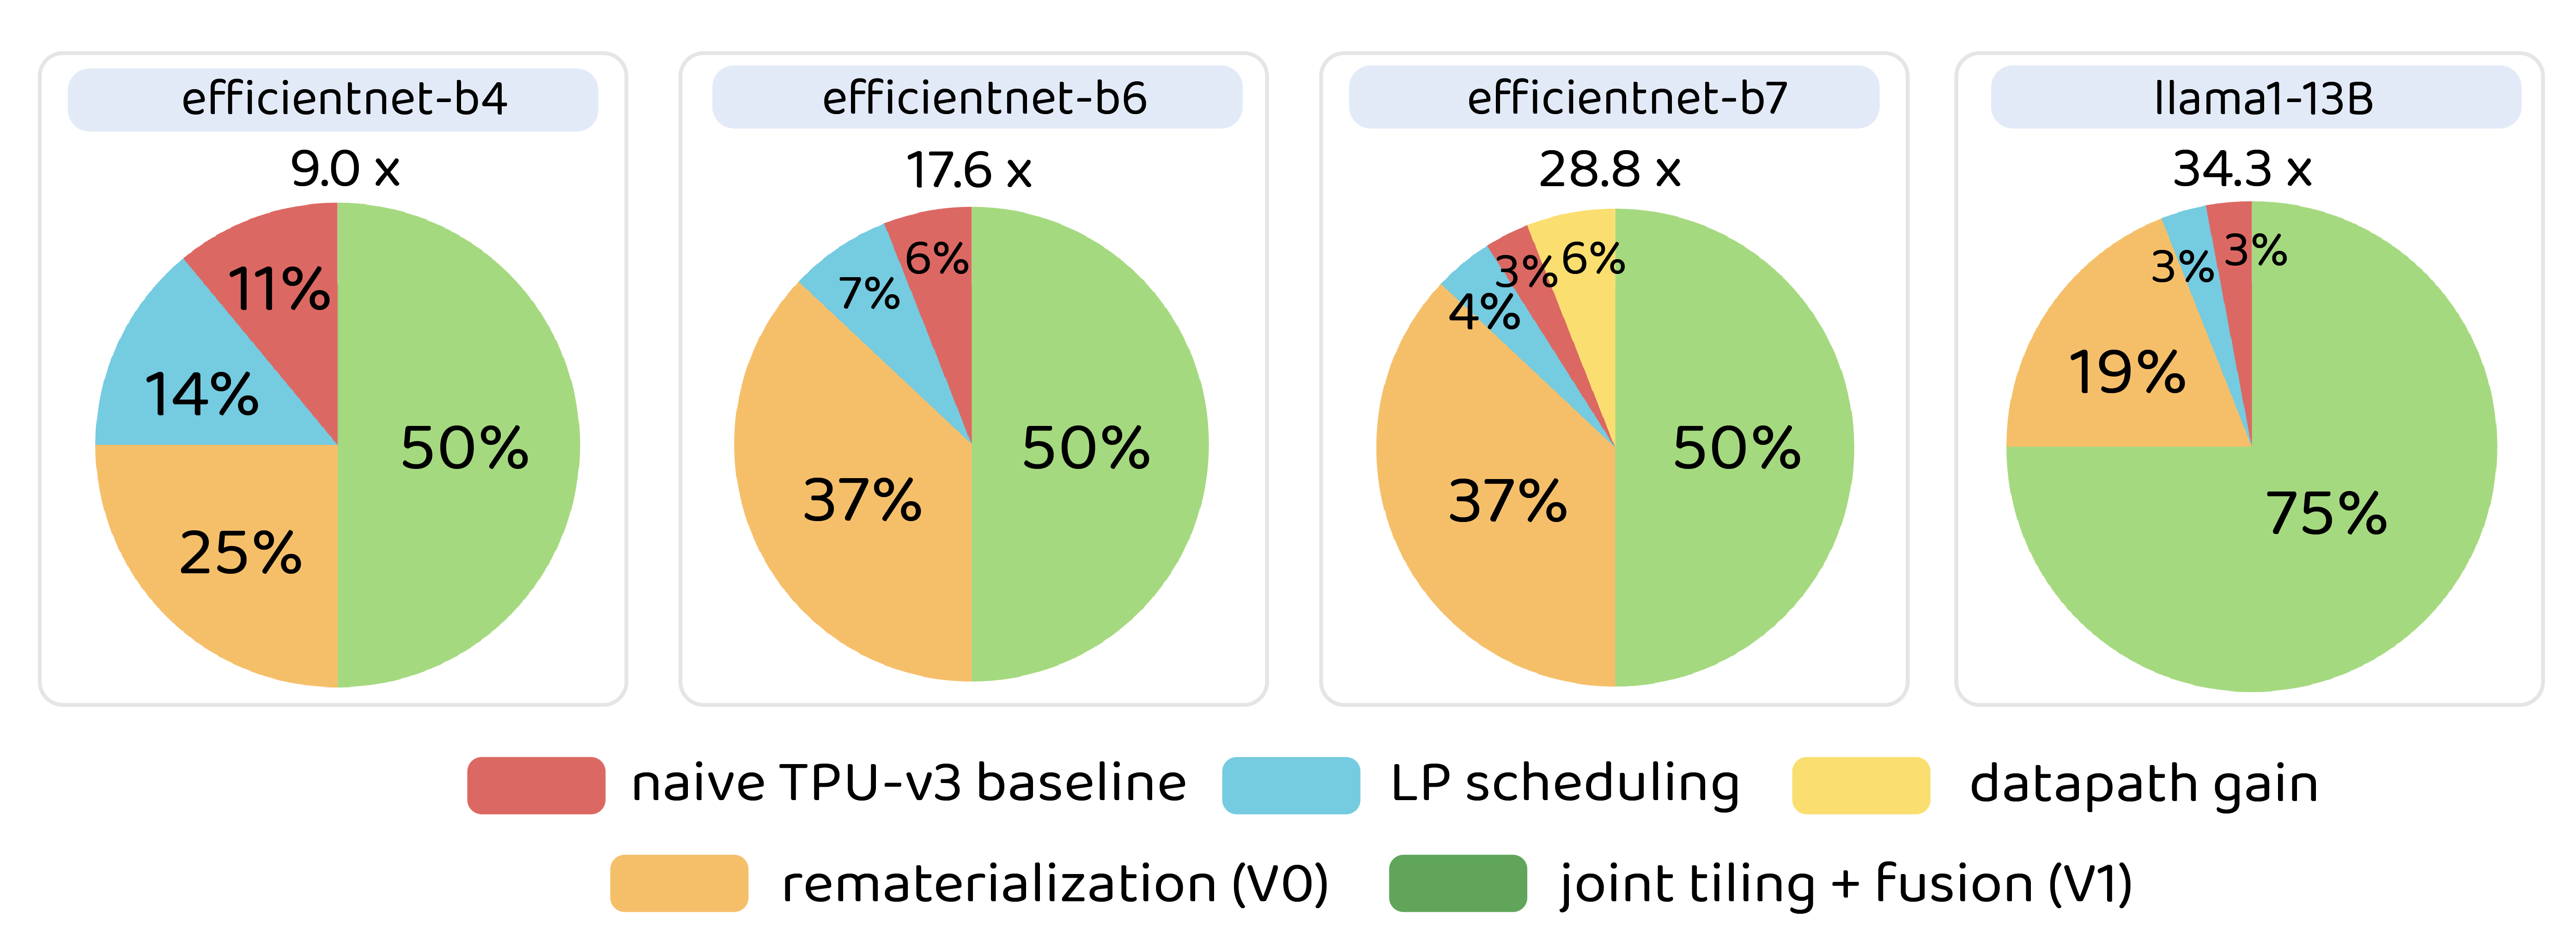
\includegraphics[width=0.85\linewidth]{fig3/speedup_decomposition_final_v4.png}
\caption{Retained historical prefill attribution under the original campaign's numerical and traffic conventions. The artwork's V1 label denotes joint tiling and fusion. New uniform BF16 phase and feature controls are reported separately in Tables~\ref{tab:uniform_llama_phases}, \ref{tab:uniform_llama_controls}, and \ref{tab:uniform_bf16_cnn_controls}.}\label{fig:accel_decompose}
\end{figure}

\begin{figure}[ht!] 
    \centering
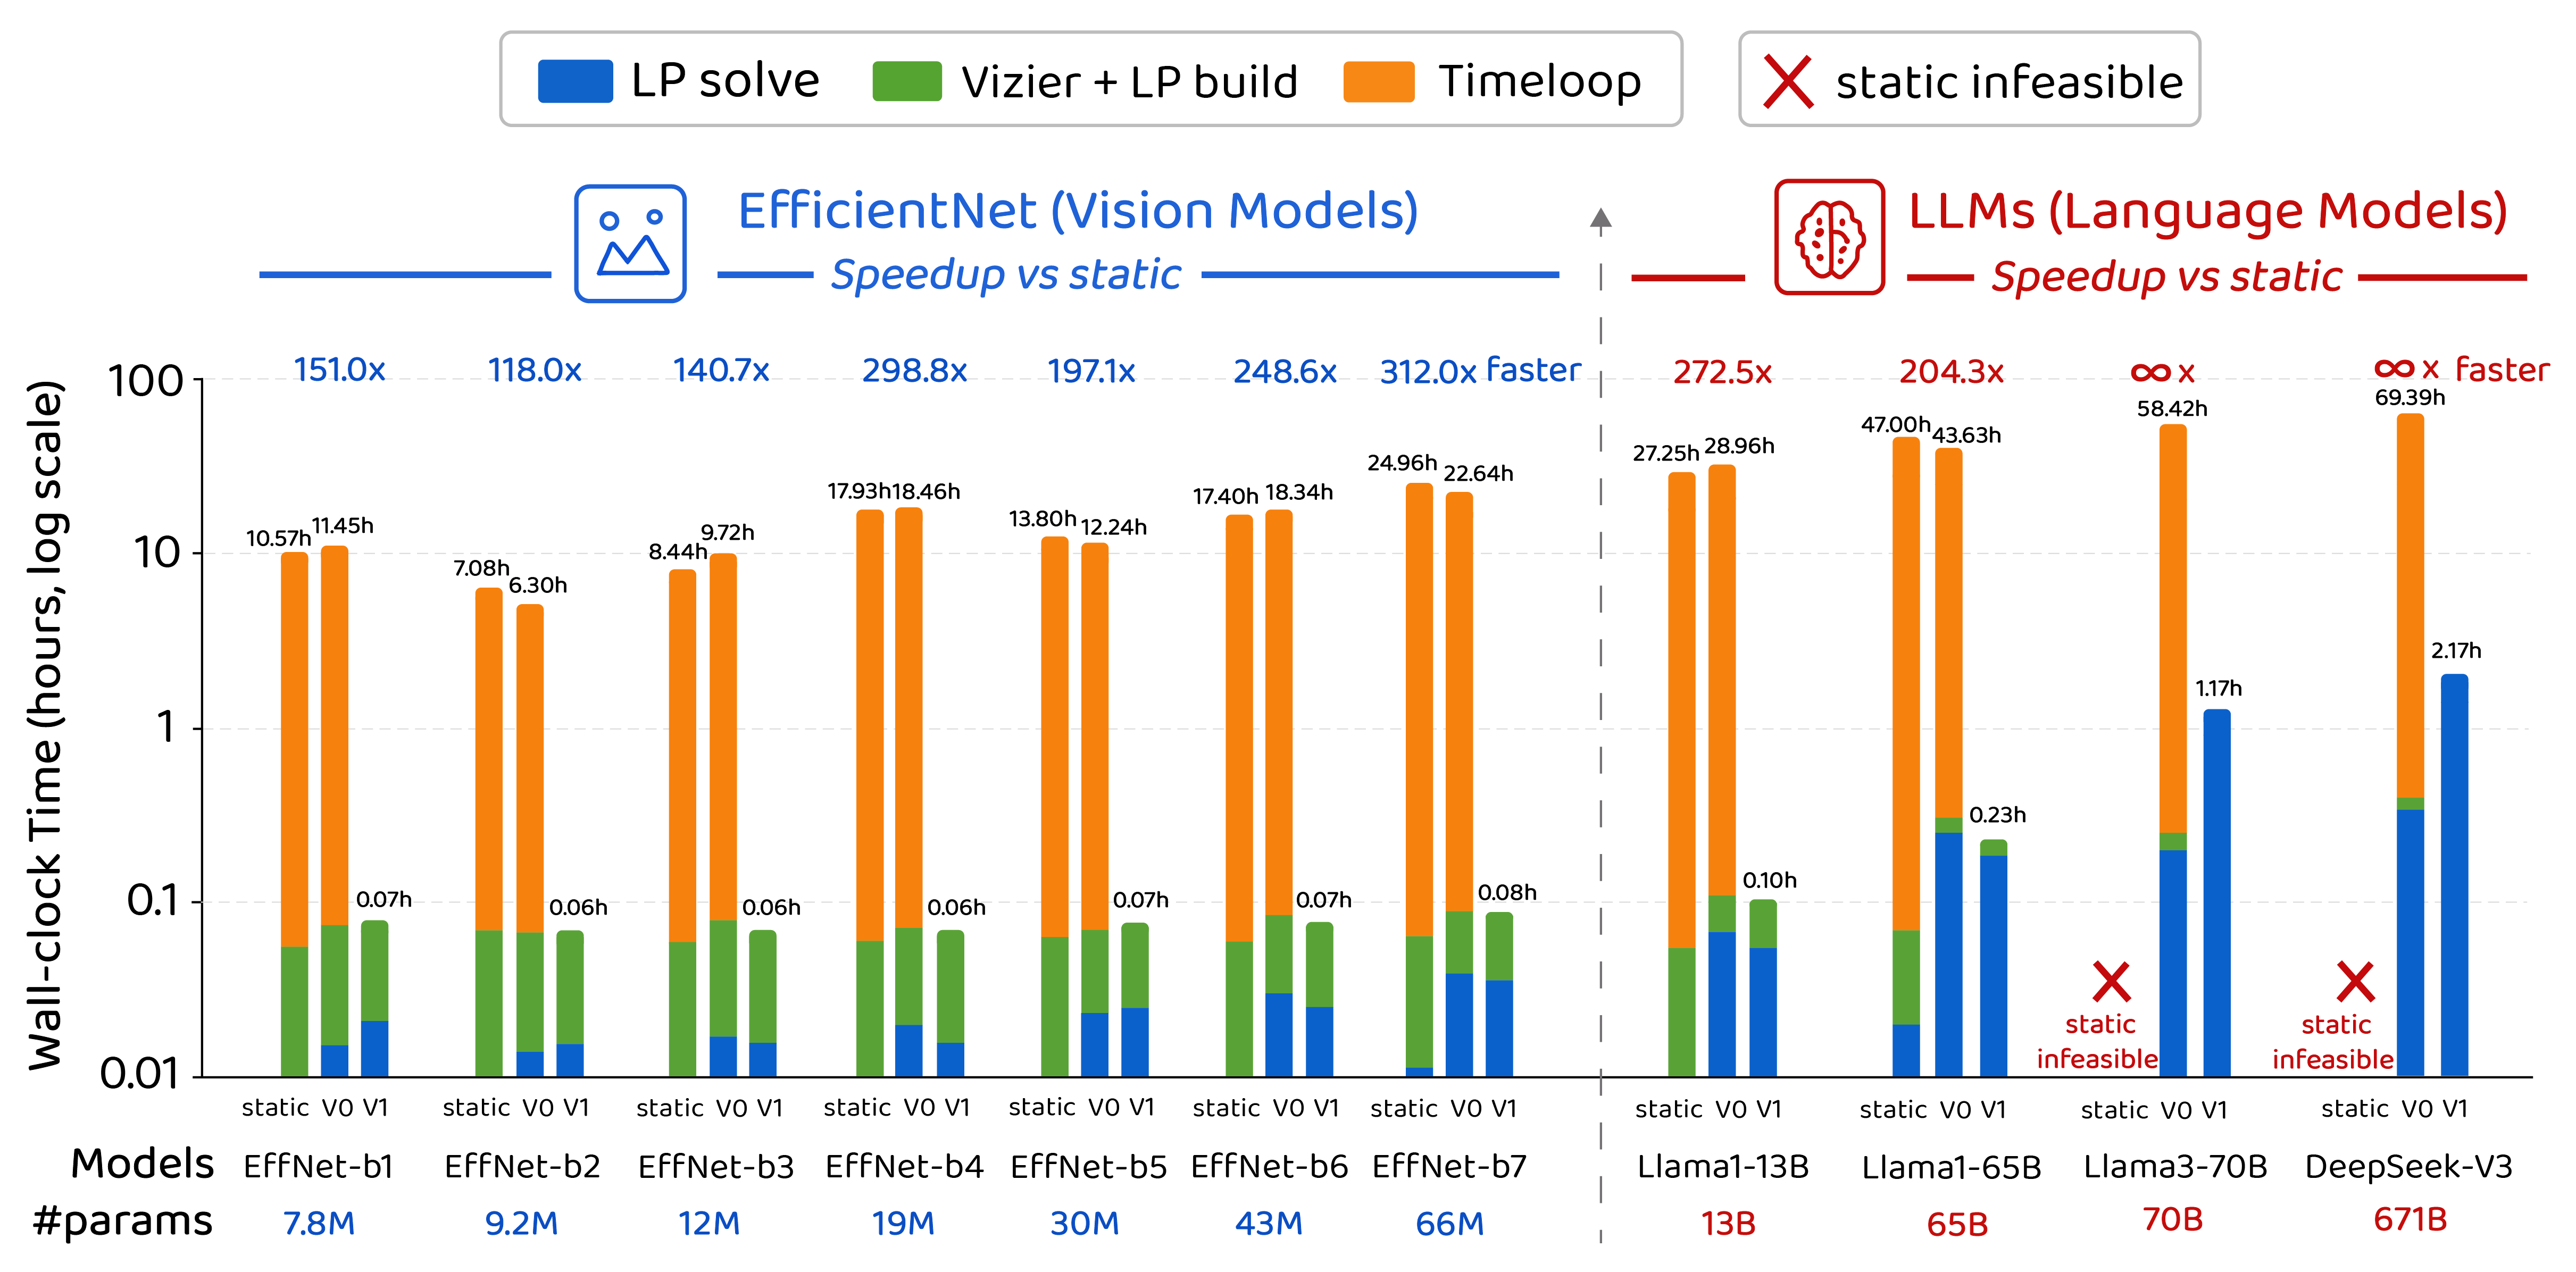
\includegraphics[width=1.0\linewidth]{fig3/wallclock_new_v6.png}
\caption{Wall-clock time decomposition and performance acceleration across formulations: CHEETAH-V1's internalized tiling eliminates the Timeloop bottleneck, achieving up to 100--300$\times$ faster search than the classical static method. Upper bars show wall-clock hours (log scale); annotations show speedup vs.\ static.}
\label{fig:wallclock}
\end{figure}

\begin{figure}[h]
\centering
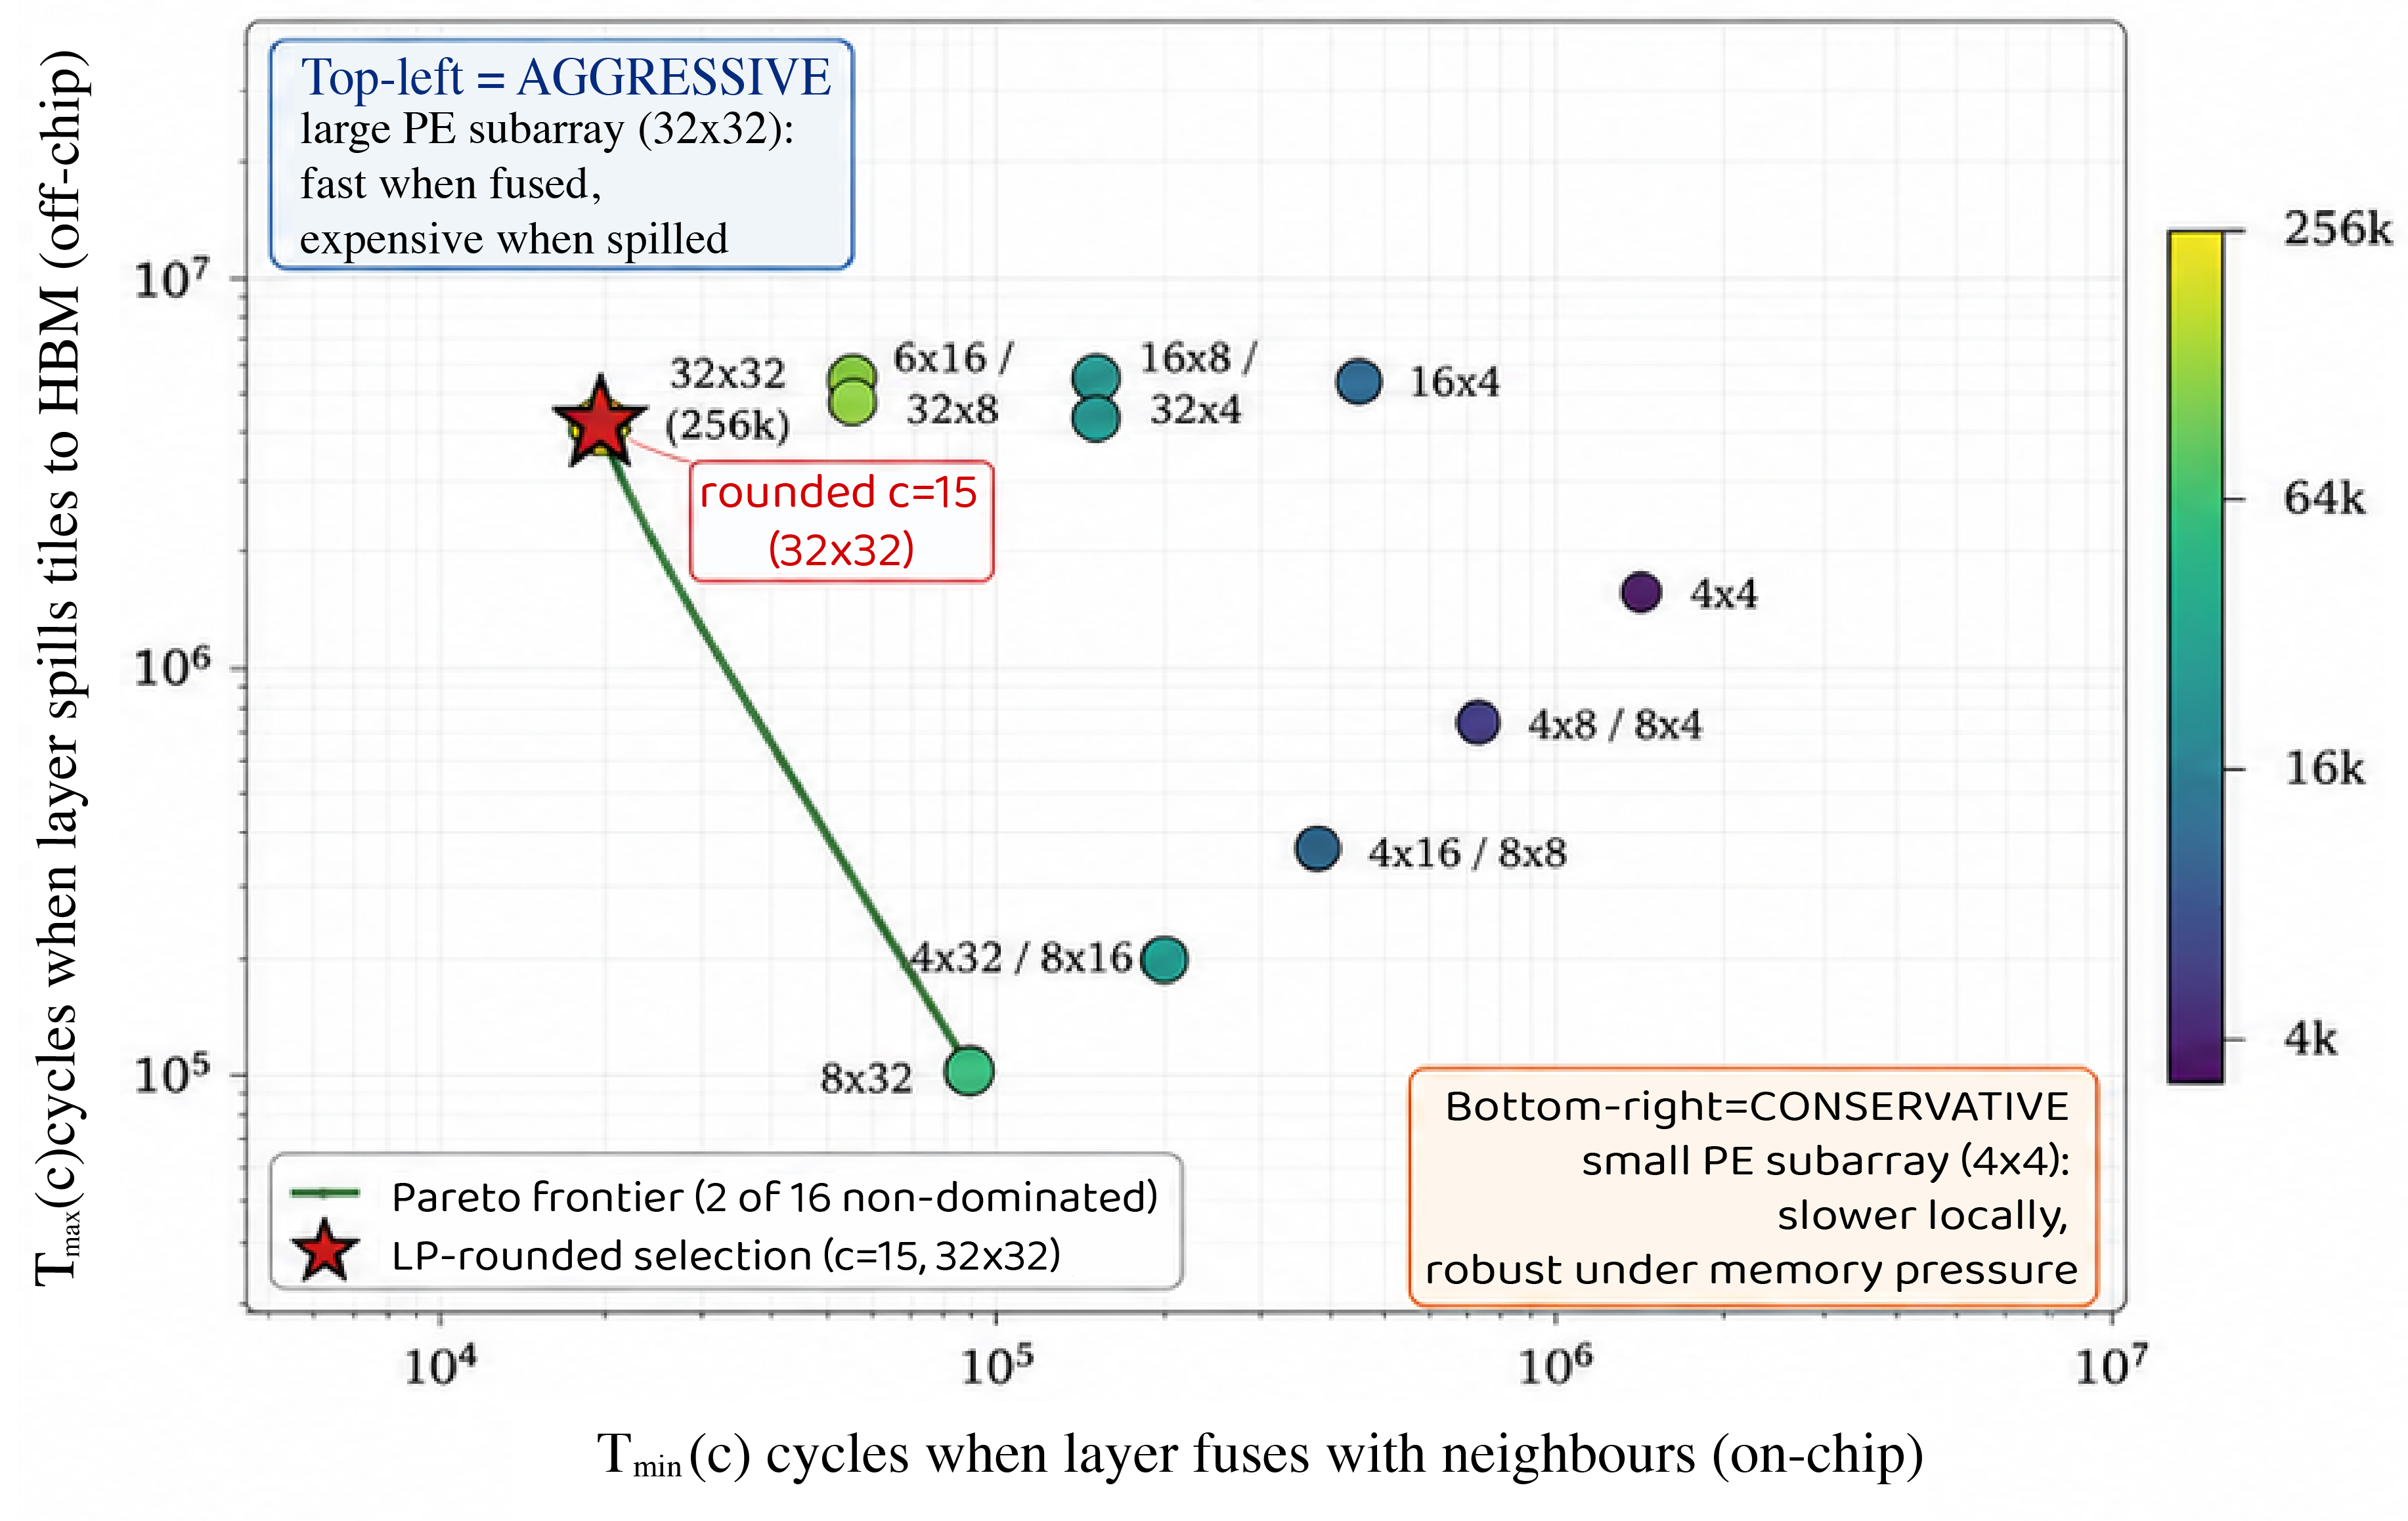
\includegraphics[width=0.48\textwidth]{figs4/pareto_front.png}
\hfill
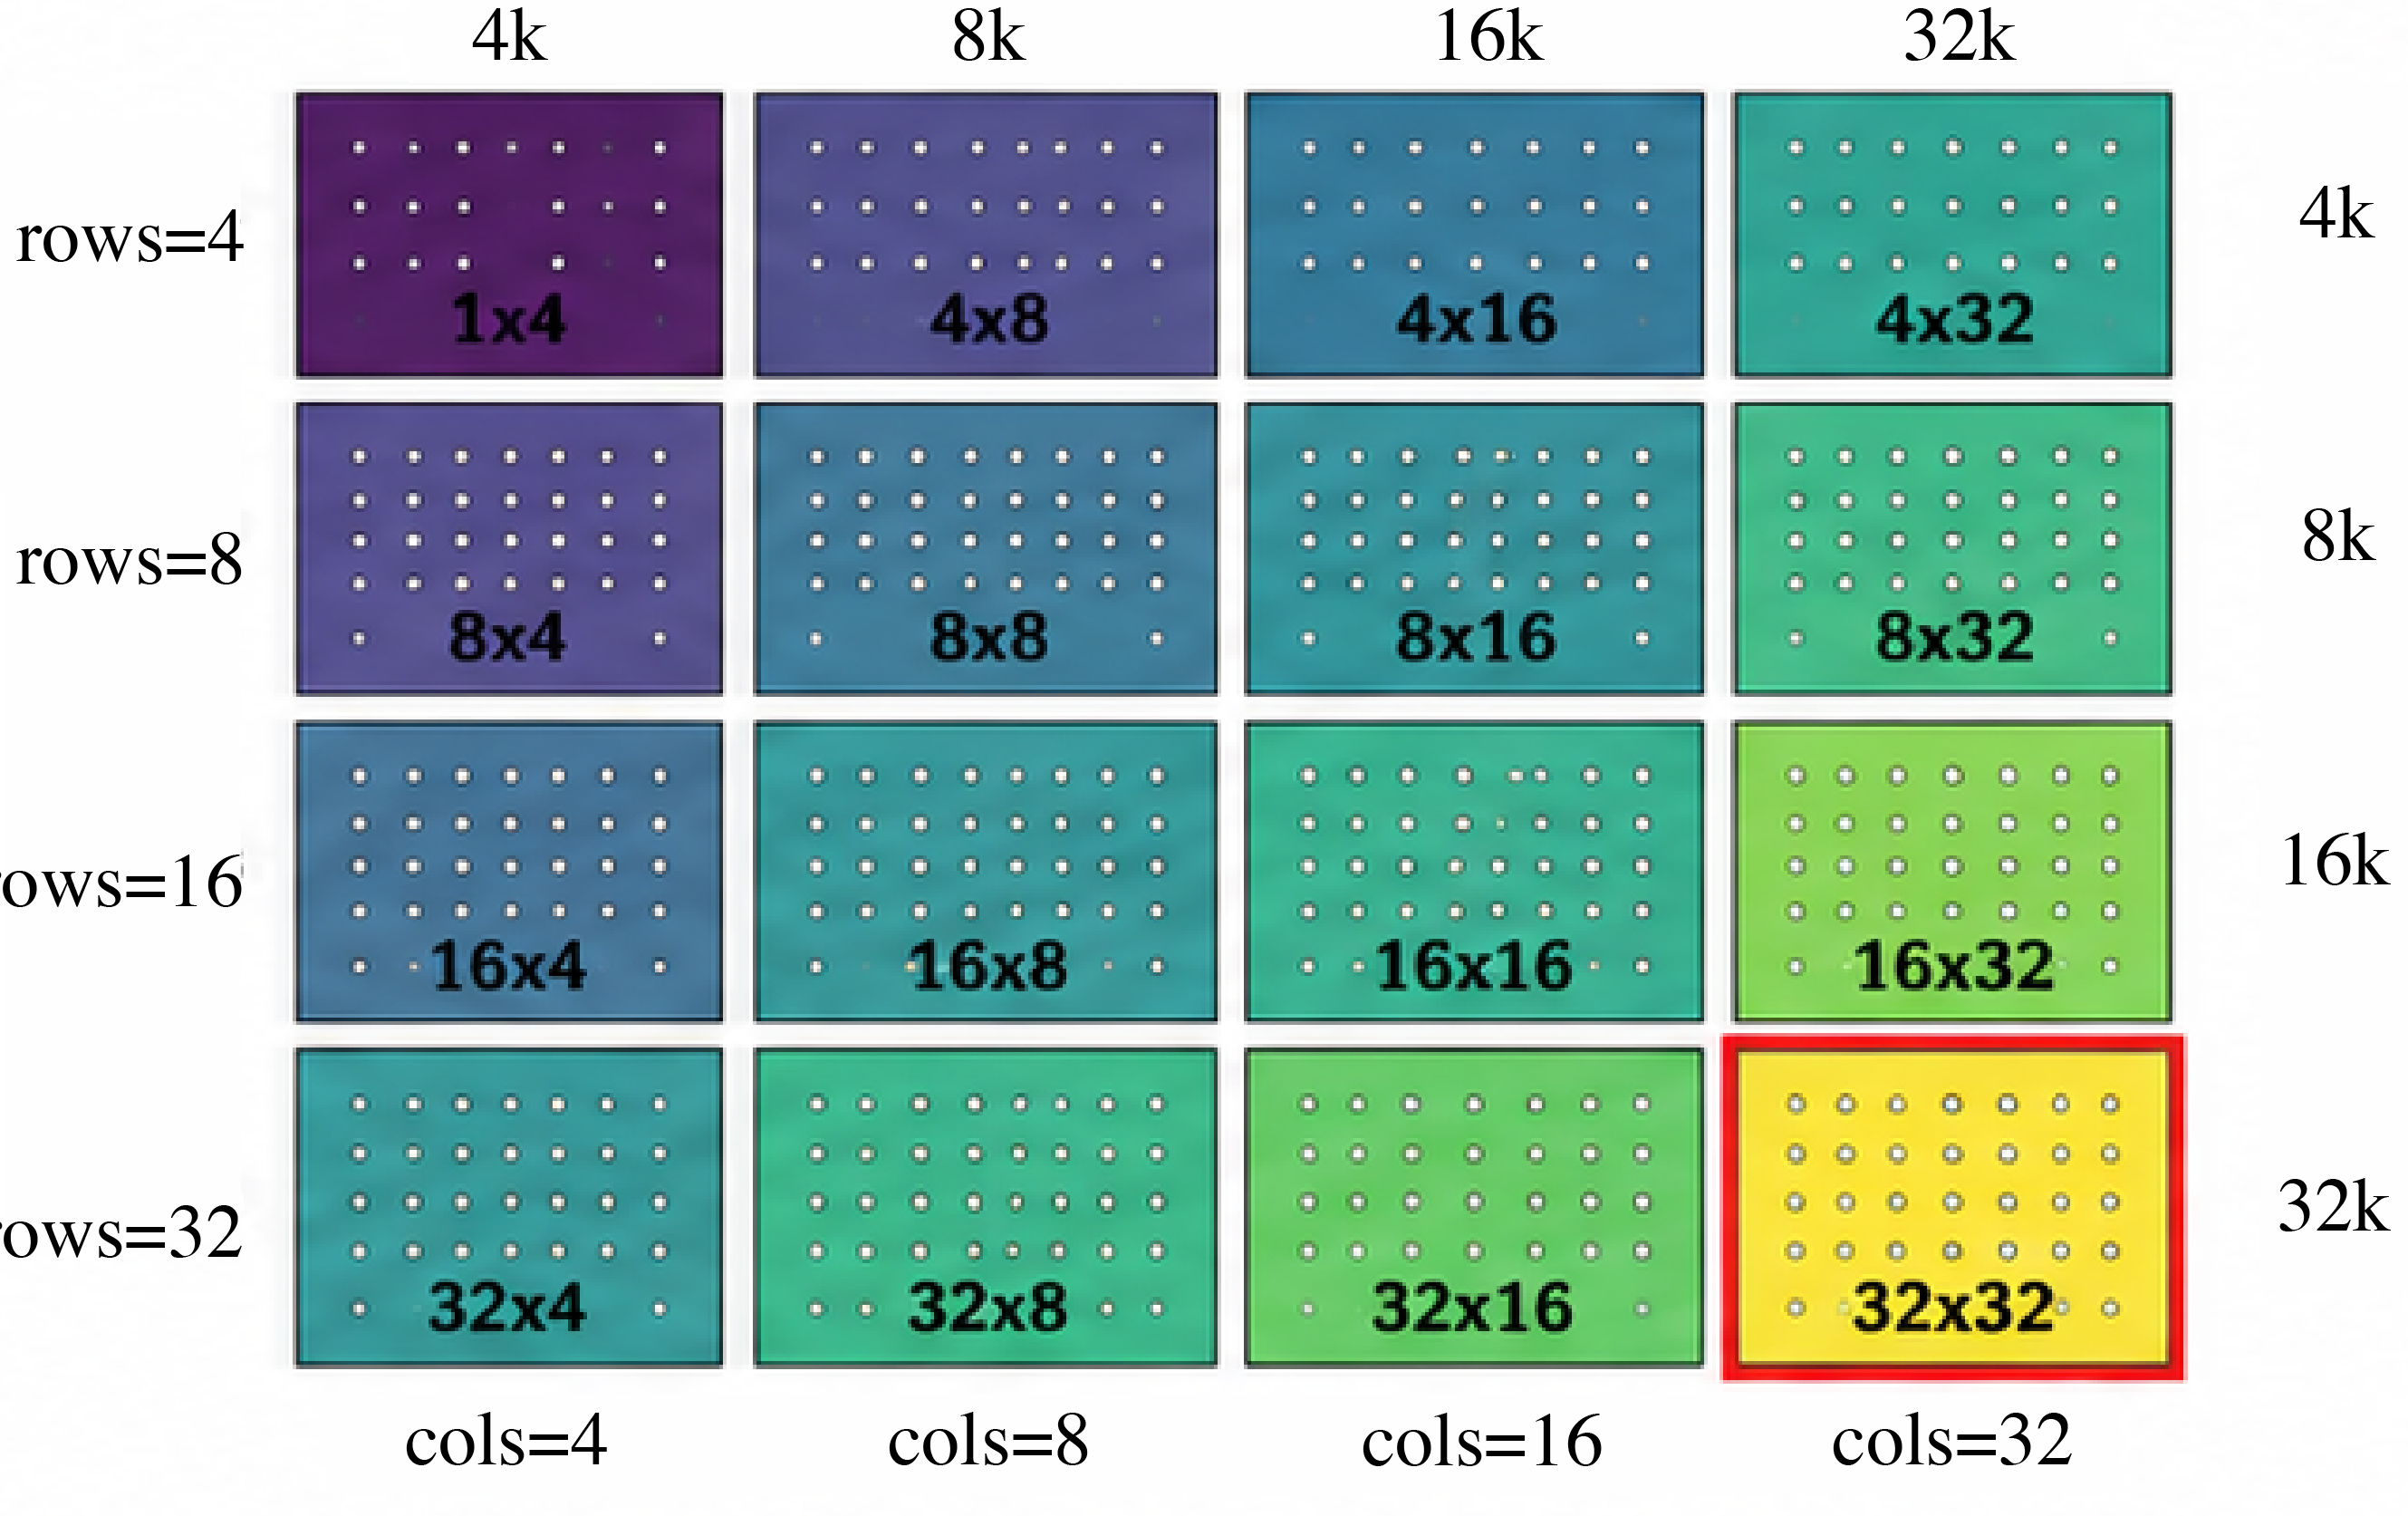
\includegraphics[width=0.48\textwidth]{figs4/tiles.png}
\caption{
Example per-layer tiling cache for EfficientNet-B7 layer L4.
Left: Timeloop-evaluated candidates plotted by fused/on-chip cost
\(T_{\min}(c)\) and spilled/off-chip cost \(T_{\max}(c)\); the frontier shows
non-dominated choices and the star is the LP-rounded selection. Right: the
16 tiling choices; labels such as \(4\times4\),
\(8\times8\), and \(32\times32\) denote active tile rows/columns inside the
fixed accelerator, white dots indicate active PE/MAC sites.
These are schedule choices, not different chips.
}
\label{fig:tiles}
\end{figure}

\begin{figure}[ht!]
    \centering
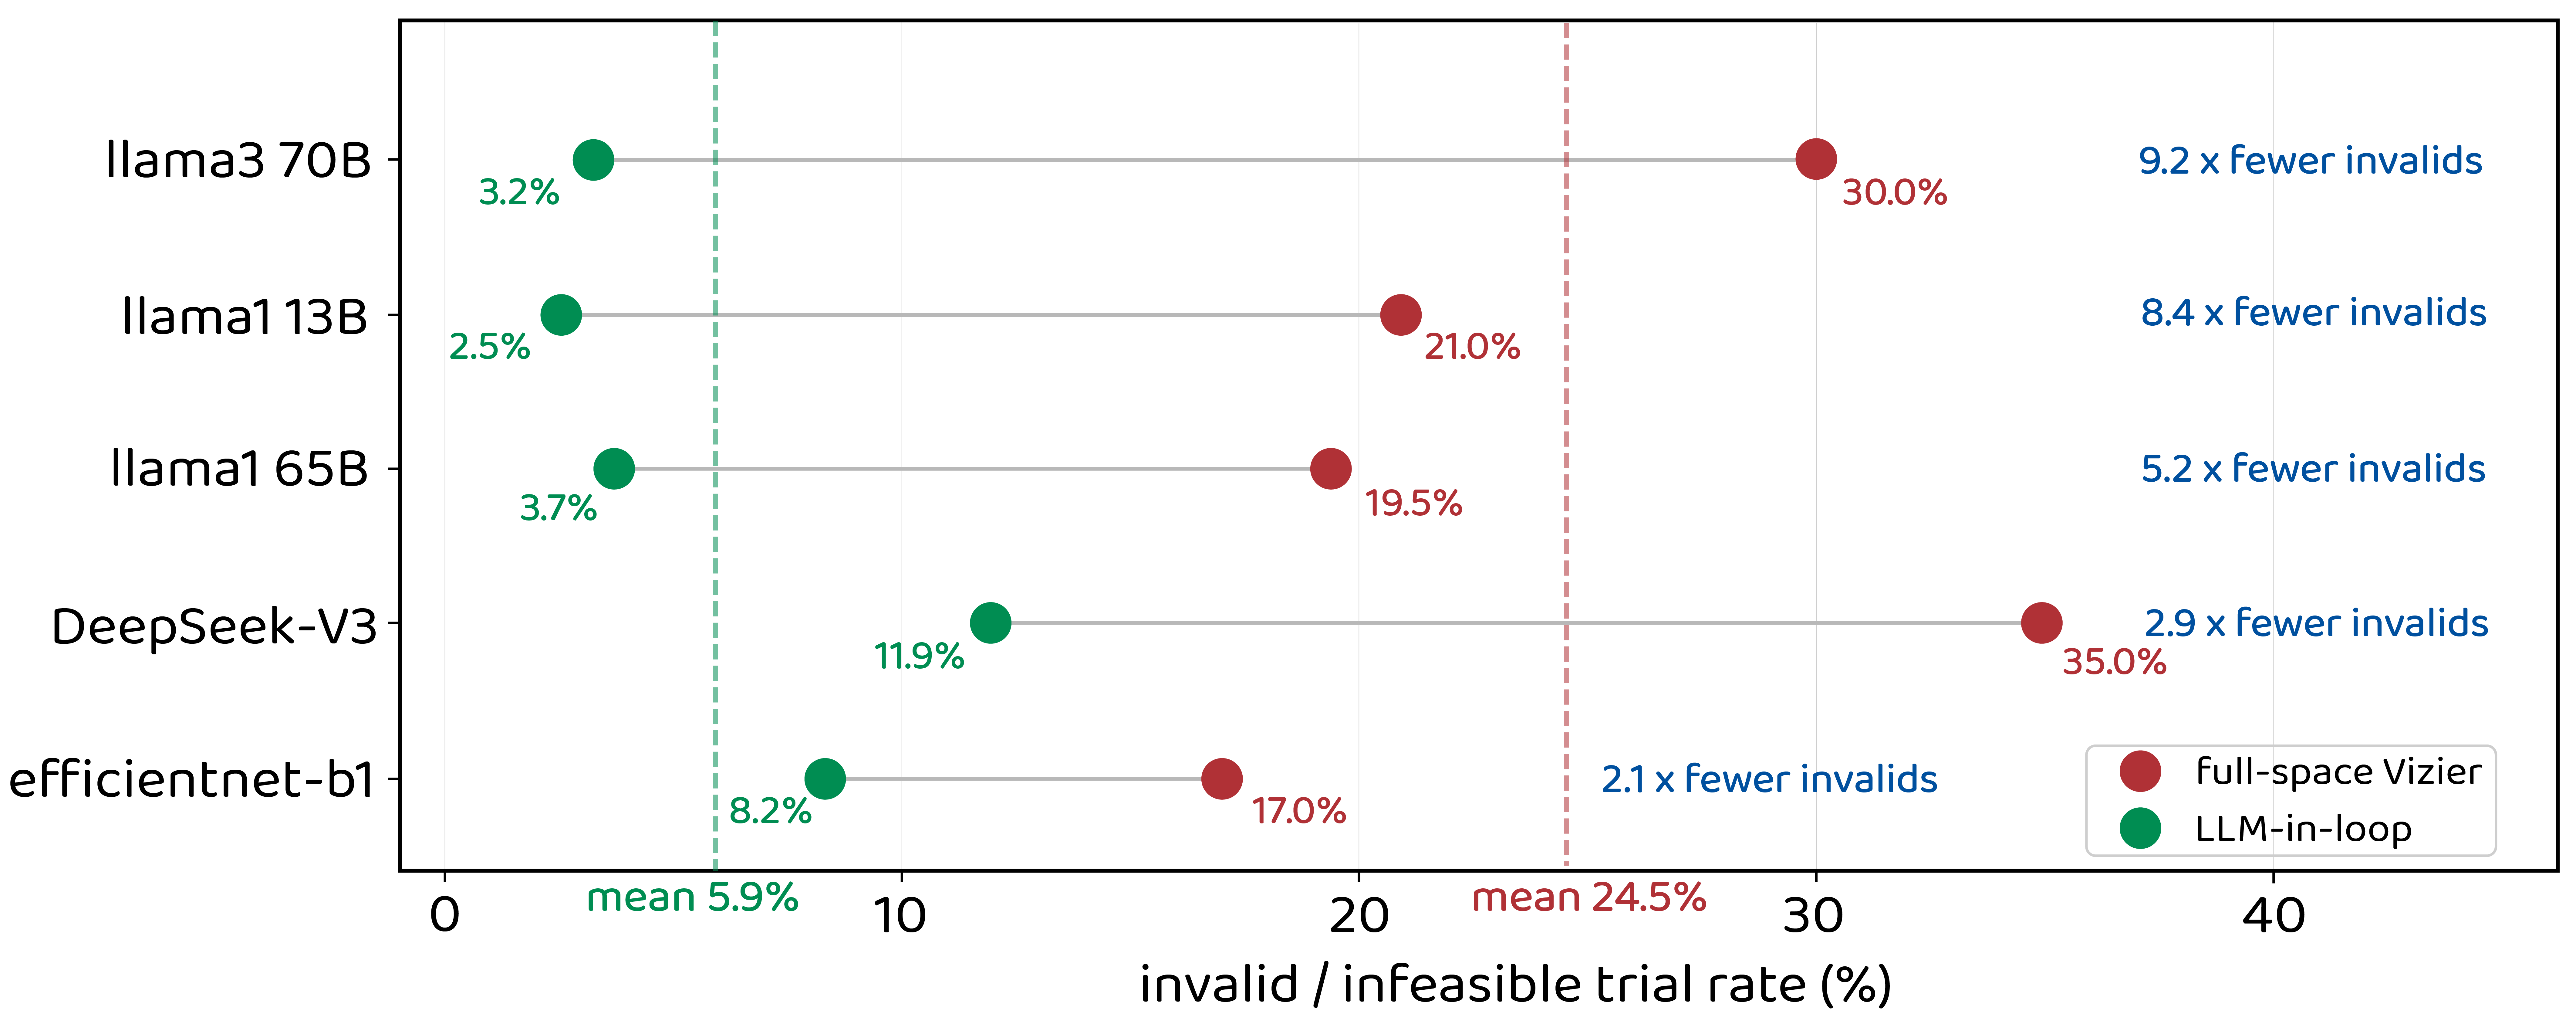
\includegraphics[width=0.85\linewidth]{fig3/llm_guide_v1.png}
\caption{Invalid/infeasible trial rate (\%) for full-space Vizier vs.\ LLM-in-loop across five workloads. The LLM Architect reduces the mean invalid rate from 24.5\% to 5.9\% (4.1$\times$ reduction), with the largest gains on LLM workloads where the hardware search space is most prone to infeasible configurations.}\label{fig:llm}
\end{figure}

\subsection{Full-Inference DeepSeek: One Chip, Prefill and Decode}
\label{sec:decode_decomp}\label{sec:batch_sensitivity}
We evaluate DeepSeek-V3 on 32 independent requests, each with 4,096 prompt
and 512 output tokens. All 61 layers execute: prefill produces the first
output, followed by 511 decode forwards. Captured expert IDs and routing
weights define all $61{,}985{,}244$ invocations in $41{,}924{,}510$ execution
groups. Original FP8 weights are converted to BF16 with the captured rounding
policy; higher-precision tensors and complete KV history are preserved.

The recovered chip has 320 $16\times16$ MAC arrays, 5,248 vector lanes,
1,024 paid FP8 receiver lanes, 78.25 MiB SRAM, 64 GiB DRAM and 2 TiB backing.
At a 1 ns analytical clock, the corrected chip provides 1,630 GB/s DRAM,
640 GB/s external and 20,480 GB/s local service. It passes the shared BF16
scenario's area, peak-power, density, pins, bank, depth and NoC predicates:
$321.69$ mm$^2$ and $298.69$ W. The BF16 peak coefficient is 1.2 mW/MAC;
the area scale and interface organization remain explicit concept assumptions,
not calibrated silicon estimates. Retiming preserves the original cover,
addresses and outer dependency order; 384 regenerated pipeline recipes pass
replay, and all other durations are conservatively extended.
The historical TPU-v3 extension retains the reference compute/DRAM resources
with 32 GB/s external and 8,192 GB/s local service, and 2,048 primitive vector
cycles/ns. These interface assumptions are explicit parts of the prediction,
not measurements of a calibrated TPU serving stack or fabricated custom chip.
This extension is not yet a verified reconstruction of FAST's modeled TPU-v3
baseline, which includes ordinary XLA fusion. The ratios below use that
retained reference with the corrected custom chip; they remain conditional
comparisons, not established reproduction of FAST's modeled TPU-v3 baseline.

\begin{table}[t]
\centering\small
\caption{Corrected custom-chip predictions (seconds); ratios use the retained, uncalibrated TPU-v3 extension.}
\label{tab:native_phases}
\begin{tabular}{@{}lrrr@{}}
\toprule
Phase & TPU-v3 extension & Custom chip & Speedup \\
\midrule
Prefill & 13,387.193 & 1,078.914 & $12.408\times$ \\
Decode & 53,083.324 & 2,074.999 & $25.582\times$ \\
Preparation & 131.252 & 42.973 & $3.054\times$ \\
\midrule
Total & 66,601.769 & 3,196.886 & $\mathbf{20.833\times}$ \\
\bottomrule
\end{tabular}
\end{table}

Phase times add; speedup is the ratio of total predicted inference latencies.
Decode contributes $80.45\%$ of time saved, prefill $19.41\%$, and preparation
$0.14\%$. Initial conversion is charged in preparation; subsequent streamed
conversion is charged to the consuming kernels. Optimization time is separate.
The retained execution's state replay is reused with the checked retiming;
the corrected fixed-chip LP separately has a $0.0846842\%$ objective interval
(Appendix~\ref{app:corrected_native_lp}). Neither this interval nor the
retiming establishes global integral optimality.

\subsection{Feature Contributions on the Same Chip}
\label{sec:native_features}
Table~\ref{tab:native_features} retains the archived chip and removes one
mechanism at a time on the original numerical workload. These are matched
execution controls, not globally optimized feature-off designs. Interacting
rows are not an additive attribution of the headline speedup. They have not
been retimed to the corrected chip in Table~\ref{tab:native_phases}.

\begin{table}[t]
\centering\small
\caption{Archived-chip feature controls: predicted time saved (seconds).}
\label{tab:native_features}
\begin{tabular}{@{}lrr@{}}
\toprule
Feature & Prefill & Decode \\
\midrule
Matrix batching & 43.173 & 856.070 \\
SwiGLU primitive fusion & 14.579 & 1.819 \\
Other elementwise register storage & 257.071 & 34.026 \\
Full-K panel reuse & 32.445 & 0 \\
Per-use weighted decode tiles & 0 & 0.866 \\
Optional KV residency & 0 & 15.726 \\
Phase-reused placement (included above) & 0 & 3.698 \\
\bottomrule
\end{tabular}
\end{table}

\paragraph{Batching and storage fusion.}
The no-batch control executes every original member separately and reselects
its tile. Resident weights remain resident; each streamed member pays its own
receive. The control expands to exactly $61{,}985{,}244$ kernels and takes
$2{,}999.864$ seconds, versus $2{,}100.621$ with batching. Thus grouped execution
and shared streamed-weight delivery give $1.612\times$ decode and
$1.064\times$ prefill gains. SwiGLU and elementwise storage choices remove
primitive spills while retaining arithmetic, BF16 rounding, and local/vector
service. Full-K panels reuse weights across output-row tiles, paying SRAM and
serialized panel waves. Holding one tile fixed per parameter family adds $0.866$ seconds to decode;
panel boundaries, buffers and residency stay fixed. This tests weighted decode
tile adaptation, rather than every temporal choice in the master.

\paragraph{KV and time-indexed placement.}
Every arm retains complete cached decoding, growth, host backing and mandatory
writes. Optional DRAM residency selects 246 request/layer/K-or-V prefix chains
and pays 125,952 copies. A fixed whole-task partition fits 193 chains; releasing
prefill temporaries before decode permits 246. Placement's $3.698$-second gain
is included in the $15.726$-second KV gain. These modest marginal gains reflect
limited DRAM capacity and the wide custom external interface. Independent
checks replay changed copies and kernel traffic; Appendix~\ref{app:native_provenance}
records exact inputs, costs, controls and their scope.



\section{Conclusion}
\label{sec:conclusion}
CHEETAH jointly represents hardware, implementation, and temporal memory
choices in one master LP relaxation. Operator-based optimization, checked
bounds, and integral replay produce concrete designs. Extending the original
prefill results, full-input DeepSeek predicts $22.88\times$ overall acceleration
under the declared TPU-v3 model, with separate phase and feature controls.
Complete pricing and broader implementation coverage remain open.




\label{page:main-end}
\clearpage
\bibliographystyle{abbrvnat}
\bibliography{ref}

\newpage
\appendix

\startcontents[appendix]
{\noindent\normalsize\textbf{Appendix}\par}
\vspace{2pt}
\begin{center}{\Large\textbf{Table of Contents}}\end{center}
\vspace{4pt}
\printcontents[appendix]{}{1}{\setcounter{tocdepth}{3}}
\clearpage

\section{Total Cost of Ownership and Return on Investment}
\label{sec:tco}
% \Vzero/\mathrm{N7} are defined in the main preamble; guard \mathrm{N5} so this fold
% is self-contained. \providecommand does not clobber an existing def.


A co-designed accelerator only pays for itself if the recurring efficiency it
buys eventually amortizes its one-time silicon cost. To evaluate this we adopt
FAST's total-cost-of-ownership (TCO) methodology~\citep{zhang_fast}
\emph{verbatim} (the same cost model, the same non-recurring-engineering (NRE)
decomposition, and the same return-on-investment (ROI) break-even analysis;
their Eq.~1--2 and Sec.~5.1), so that our deployment economics are read on
FAST's own terms and are directly comparable to their Table~4. We stress at the
outset that this is the weakest-grounded part of our evaluation: absolute TCO
depends on proprietary fleet data neither we nor FAST possess, several cost
constants are assumption-flagged, and the speedup that drives the ROI depends
strongly on which baseline it is measured against. We therefore do not report a
single $S$: \cref{par:tco_nonparity} stratifies every Perf/TDP figure over three
denominators of increasing strength, and we carry the ROI through on the design
that clears the strongest of them (\cref{par:tco_iso}), stating plainly that the
throughput-provisioned blueprints do not. We report ROI as an order-of-magnitude
plausibility check, not a precise claim, and we state every caveat inline.

\paragraph{FAST's cost model (what we mirror).}
FAST models the three-year cost of a fleet that offloads $n$ baseline
accelerator-units of traffic onto a co-designed chip as
%
\begin{equation}
\label{eq:tco_old}
\mathrm{TCO}_{\mathrm{old}}(n) \;=\; C_{\mathrm{cap}}(n) \;+\; t_D\, C_{\mathrm{op}}(n),
\end{equation}
%
capital cost plus lifetime ($t_D=3$~yr) operating cost, and defines the ROI of
committing the co-design NRE as
%
\begin{equation}
\label{eq:tco_roi}
\mathrm{ROI} \;=\; \frac{\mathrm{TCO}_{\mathrm{old}}\,(S-1)}
{\bigl(t_{\mathrm{design}}\,C_{\mathrm{eng}} + C_{\mathrm{mask}} + C_{\mathrm{IP}}\bigr)\,S},
\end{equation}
%
where $S$ is the per-unit efficiency gain of the co-designed chip over the
baseline; $\mathrm{ROI}>1$ means the deployment is profitable. Because per-chip
TCO is confidential, FAST uses $S=\text{Perf/TDP}$ as a proxy for Perf/TCO (the
two are reported to be highly correlated for datacenter
accelerators~\citep{jouppi2017datacenter,jouppi2021ten}) and anchors the
baseline unit to a commodity DGX-A100 accelerator. We reuse this proxy, this
DGX-anchored baseline unit, and FAST's engineering-NRE constant
($t_{\mathrm{design}}\,C_{\mathrm{eng}}=\text{65 engineer-years}\times\$240\mathrm{K}\times1.65$
overhead $=\$25.74\mathrm{M}$) unchanged. Inverting \cref{eq:tco_roi} at a
target ROI multiple $R$ gives the break-even deployment volume
%
\begin{equation}
\label{eq:tco_breakeven}
n^\star(R) \;=\; \frac{R\,\cdot\,\mathrm{NRE}\,\cdot\,S}{(S-1)\,\cdot\,\mathrm{TCO}_{\mathrm{unit}}},
\qquad
\mathrm{NRE} = t_{\mathrm{design}}\,C_{\mathrm{eng}} + C_{\mathrm{mask}} + C_{\mathrm{IP}},
\end{equation}
%
the number of baseline units whose traffic must be offloaded before the NRE is
repaid. All arithmetic below is a pure evaluation of
\cref{eq:tco_old,eq:tco_roi,eq:tco_breakeven} on the eight co-designed
blueprints of \cref{app:blueprints}; no solver is involved.

\paragraph{Break-even under FAST parity.}
Under FAST's Perf/TDP proxy, our co-designed chips retain
$S=1.15\text{--}1.79\times$ Perf/TDP over a modeled TPU-v3 after normalizing away
raw MAC scale, measured against the c0-naive denominator (D1) of
\cref{par:tco_nonparity}. These are \emph{prefill} blueprints under that
convention. The iso-resource analysis of \cref{par:tco_iso} separately compares
against a well-scheduled baseline; neither calculation uses the native
full-inference timings. For the best chip (the DeepSeek-V3~\citep{deepseekv3report}
$\mathrm{N7}$ design on TSMC~N7 with LPDDR5X, $S=1.79$), \cref{eq:tco_breakeven} gives a
$1\times$-ROI break-even of $\mathbf{4{,}410}$ units (\cref{tab:tco_breakeven},
\cref{fig:tco_breakeven}). This sits at the \emph{same order of magnitude} as
FAST's own reported $2{,}164\text{--}3{,}534$ units (their Table~4, at
$S=1.84\text{--}3.91$), and well within the thousands-to-tens-of-thousands scale
of modern accelerator fleets. As \cref{eq:tco_breakeven} makes explicit and
\cref{fig:tco_breakeven} shows, deployment volume dominates ROI: the ranking of
chips by break-even volume is driven jointly by $S$ and by NRE, and the
N7-plus-commodity-memory family ($\mathrm{N7}$) is uniformly ROI-preferred over the
N5-plus-HBM3 family ($\mathrm{N5}$), which carries ${\sim}\$15\mathrm{M}$ more mask NRE,
$1.7\text{--}2.5\times$ the unit TCO, and (except on the 13B) \emph{lower}
Perf/TDP, pushing its break-even to $13{,}000\text{--}19{,}000$ units.

\begin{table}[t]
\centering
\small
\caption{FAST-parity break-even volumes (convention F: $S=\text{Perf/TDP}$
proxy, DGX-A100-anchored baseline unit), computed from
\cref{eq:tco_breakeven}. NRE is $\$50.7\mathrm{M}$ for the N7 ($\mathrm{N7}$) family
and $\$65.7\mathrm{M}$ for the N5+HBM3 ($\mathrm{N5}$) family. For reference, FAST's
Table~4 reports $1\times$-ROI volumes of $2{,}164\text{--}3{,}534$ units at
$S=1.84\text{--}3.91$. Cost constants are assumption-flagged; see
\cref{par:tco_nre}.}
\label{tab:tco_breakeven}
\begin{tabular}{@{}llrrrr@{}}
\toprule
\textbf{Chip (blueprint)} & \textbf{Process / memory} & $\mathbf{S}$ &
\textbf{1$\times$} & \textbf{2$\times$} & \textbf{4$\times$} \\
\midrule
DeepSeek-V3 $\mathrm{N7}$ & N7 / LPDDR5X & $1.79$ & $\mathbf{4{,}410}$ & $8{,}821$ & $17{,}641$ \\
Llama1-65B $\mathrm{N7}$  & N7 / LPDDR5X & $1.74$ & $4{,}591$ & $9{,}182$ & $18{,}363$ \\
Llama3-70B $\mathrm{N7}$  & N7 / LPDDR5X & $1.54$ & $5{,}528$ & $11{,}057$ & $22{,}114$ \\
Llama1-13B $\mathrm{N5}$  & N5 / HBM3    & $1.57$ & $6{,}920$ & $13{,}841$ & $27{,}681$ \\
Llama1-13B $\mathrm{N7}$  & N7 / GDDR6X  & $1.42$ & $6{,}641$ & $13{,}283$ & $26{,}566$ \\
DeepSeek-V3 $\mathrm{N5}$ & N5 / HBM3    & $1.24$ & $13{,}083$ & $26{,}166$ & $52{,}332$ \\
Llama1-65B $\mathrm{N5}$  & N5 / HBM3    & $1.20$ & $15{,}079$ & $30{,}158$ & $60{,}317$ \\
Llama3-70B $\mathrm{N5}$  & N5 / HBM3    & $1.15$ & $19{,}237$ & $38{,}473$ & $76{,}947$ \\
\bottomrule
\end{tabular}
\end{table}

\begin{figure}[t]
\centering
% TODO: render from tco_data.json (fast_convention/tco_data.json,
%       breakeven_volume_conventionF, 1x_ROI per representative_chips).
%       Grouped bar chart: one bar per blueprint (8), N7/V1 vs N5/V2
%       families in two colors; y-axis = 1x-ROI break-even volume (units,
%       log or linear). Overlay a horizontal shaded band at 2,164-3,534 =
%       FAST's Table-4 range, and a dashed marker at 3,650 = our best chip
%       under FAST's implied ~$42M NRE (\cref{par:tco_nre}).
% \includegraphics[width=0.78\linewidth]{figs/tco_breakeven.pdf}
\caption{FAST-parity $1\times$-ROI break-even deployment volume per co-designed
blueprint (convention F), from \cref{eq:tco_breakeven}. The shaded band marks
FAST's own reported range ($2{,}164\text{--}3{,}534$ units); our best chip
(DeepSeek-V3 $\mathrm{N7}$, $4{,}410$ units) lands just above it, and drops to
${\sim}3{,}650$ units (\emph{inside} FAST's range) when evaluated at FAST's
implied ${\sim}\$42\mathrm{M}$ total NRE. The N7$+$commodity-memory ($\mathrm{N7}$)
family is uniformly ROI-preferred over N5$+$HBM3 ($\mathrm{N5}$).}
\label{fig:tco_breakeven}
\end{figure}

\paragraph{Reconciling the NRE.}
\label{par:tco_nre}
The NRE terms in \cref{eq:tco_breakeven} carry the largest uncertainty, and we
flag them as assumptions~[A] rather than measured quantities: the mask-set cost
($\$15\mathrm{M}$ at N7, $\$30\mathrm{M}$ at N5), the IP/PHY-licensing cost
($\$10\mathrm{M}$, ASIC-Clouds-class~\citep{magaki2016asic}), the defect density
$D_0$ used in the die-yield model, and the PUE all follow public industry-class
estimates, not vendor data. FAST published only its engineering-NRE constant, so
rather than assert NRE parity we \emph{reconcile}: back-computing from FAST's own
Table~4 break-even volumes and reported $S$ implies a FAST total NRE of
${\sim}\$42.0\mathrm{M}$. Our best chip carries a larger, deliberately
conservative $\$50.7\mathrm{M}$; re-evaluating \cref{eq:tco_breakeven} at FAST's
implied ${\sim}\$42\mathrm{M}$ moves our best-chip break-even from $4{,}410$ to
$\mathbf{{\sim}3{,}650}$ units, now \emph{inside} FAST's own
$2{,}164\text{--}3{,}534$ range. The Perf/TDP proxy $S$ is independent of these
[A] constants except through NRE, so the headline break-even row is robust to
them: doubling the mask cost alone moves the $1\times$-ROI volume only to
${\sim}5{,}700$. We also disclose the honest error bar from the proxy itself: a
fully modeled TCO on both sides (convention M) inflates break-even to
${\sim}79{,}000\text{--}108{,}000$ units (an ${\sim}18\times$ spread), which is
precisely why FAST, and we, headline Perf/TDP and cite the Perf/TCO correlation
rather than claim TCO precision.

\paragraph{The zero-NRE deployment option.}
\label{par:tco_zeronre}
A distinct and strictly cleaner deployment story requires \emph{no silicon at
all}. Because CHEETAH's scheduler is a drop-in software layer, applying the joint
LP schedule to the \emph{existing} TPU-v3 fleet (same chip, same TDP) delivers
$S=2.14\text{--}2.51\times$ Perf/TDP on the LLM workloads ($2.21\times$ on
EfficientNet-B7~\citep{tan2019efficientnet}, $1.50\times$ on the Stable-Diffusion
U-Net) at software-only engineering cost, with $C_{\mathrm{mask}}=C_{\mathrm{IP}}=0$
(\cref{fig:tco_perftdp}). Under \cref{eq:tco_roi} the NRE collapses to a software
term and the ROI exceeds any silicon option at every volume. This is a genuine,
low-risk path to fleet-wide efficiency that does not depend on any of the
[A]-flagged silicon constants above.

\begin{figure}[t]
\centering
% TODO: render from tco_data.json (fast_convention/tco_data.json,
%       S_conventionF_perf_per_tdp_proxy for silicon chips;
%       zero_nre_option.finding for the TPU-v3 scheduling bars) and
%       fast_convention/table5_cheetah.md. Grouped bar chart:
%       (a) co-designed silicon 1.15-1.79x Perf/TDP, (b) zero-NRE TPU-v3
%       scheduling 2.14-2.51x (LLMs) / 2.21x (B7) / 1.50x (SD), against a
%       baseline of 1.0. Annotate the ~0.8x well-scheduled-TPU-v3 line as a
%       dashed threshold (\cref{par:tco_nonparity}).
% \includegraphics[width=0.78\linewidth]{figs/tco_perf_tdp.pdf}
\caption{Perf/TDP (FAST's TCO proxy) of the two deployment options against a
TPU-v3 baseline of $1.0$. Co-designed silicon retains $1.15\text{--}1.79\times$
after normalizing away MAC scale; deploying CHEETAH \emph{scheduling} on the
existing TPU-v3 fleet delivers $2.14\text{--}2.51\times$ at zero silicon NRE. The
dashed band marks the $0.46\text{--}0.84\times$ obtained when the blueprints are
measured against a \emph{joint-scheduled} TPU-v3 (denominator (D3)) rather than a
naive one, and the marker at $3.00\text{--}3.21\times$ is CHEETAH-iso against
that same denominator (\cref{par:tco_nonparity,par:tco_iso}).}
\label{fig:tco_perftdp}
\end{figure}

\paragraph{Baseline stratification: three denominators, never mixed.}
\label{par:tco_nonparity}
Our $S$ and FAST's $S$ are \emph{not measured against the same baseline}:
CHEETAH's speedup is measured against a naive streaming schedule on the
reference hardware, whereas FAST's is measured against a production-calibrated
simulator. Rather than carry a single $S$ and a caveat, we report Perf/TDP
against three denominators of increasing strength and tag every number with the
one it uses:
%
\begin{enumerate}[label=(D\arabic*),leftmargin=*]
\item \textbf{c0-naive.} TPU-v3 running its deployed per-operation
configuration. This is the FAST-comparable ``TPU-v3 as deployed'' convention.
\item \textbf{stream-naive.} The per-operation streaming optimum
$\sum_i \min_c \max(C_{i,c}, \alpha B_{i,c})$: the strongest capacity-unaware
analytic baseline.
\item \textbf{joint-scheduled.} A TPU-v3 running \emph{CHEETAH's own} joint LP
schedule. This is the well-scheduled denominator, and it is the correct hurdle
rate for any silicon proposal, because \cref{par:tco_zeronre} shows that
schedule is available on the existing fleet at zero silicon NRE.
\end{enumerate}
%
Against (D3) the co-designed \emph{blueprints} of \cref{app:blueprints} do not
clear the bar, and we state the arithmetic rather than a rounded caveat. Their
$S=1.15\text{--}1.79\times$ is measured against (D1), while the same schedule on
unmodified TPU-v3 already buys $2.14\text{--}2.51\times$; the blueprints
therefore sit at $0.46\text{--}0.84\times$ against (D3), $S-1<0$, and
\cref{eq:tco_breakeven} admits \emph{no break-even at any deployment volume}.
That is the correct reading of those chips, and it is not a defect of the
formulation: the blueprints are provisioned for \emph{throughput}, which
\cref{app:deficit:twofactor} shows is where $20.0\text{--}26.9\times$ of their
headline comes from, and raw throughput is not what a Perf/TDP proxy rewards.
The blueprints' deployment case rests on per-chip throughput, latency, and the
consequent reduction in fleet size and footprint, mirroring FAST's own
observation that latency and model-enablement can justify even break-even ROI.
It does not rest on Perf/TDP, and we no longer claim that it does.

\paragraph{The iso-resource design does clear the bar.}
\label{par:tco_iso}
Optimizing Perf/TDP directly, under hard caps at TPU-v3's own area and TDP
budget, selects a different chip. \textbf{CHEETAH-iso} carries the \emph{same}
$65{,}536$ MACs as TPU-v3 at $0.82\times$ its area ($73.83$~mm$^2$ against an
$89.83$~mm$^2$ cap), and provisions $128$~GB/s of GDDR6 where TPU-v3 provisions
$900$~GB/s of HBM. Because it has no additional MACs, the provisioning factor
$f_2$ of \cref{app:deficit:twofactor} is eliminated \emph{by construction}, so
what it reports is attributable to the optimization rather than to silicon
scale. \cref{tab:tco_iso} evaluates it against all three denominators.

\begin{table}[t]
\centering
\small
\caption{CHEETAH-iso ($65{,}536$ MACs $=$ TPU-v3, $0.82\times$ area, $128$~GB/s)
Perf/TDP against the three denominators of \cref{par:tco_nonparity}, with the
$1\times$-ROI break-even volume from \cref{eq:tco_breakeven} computed at the
(D3) figure: the strongest baseline, a TPU-v3 running CHEETAH's own joint
schedule. NRE is held at the N7 family's $\$50.7\mathrm{M}$ even though the die
is smaller, which is conservative. FAST's Table~4 reports $2{,}164\text{--}3{,}534$
units. Richer TDP convention ($\mathrm{TDP}=\mathrm{MACs}\cdot2.3\!\times\!10^{-4}
+0.07\,\mathrm{W}/(\mathrm{GB/s})\cdot\mathrm{BW}$) applied to both sides.}
\label{tab:tco_iso}
\begin{tabular}{@{}lcccrc@{}}
\toprule
\textbf{Workload} & \textbf{(D1) c0} & \textbf{(D2) stream} &
\textbf{(D3) joint} & \textbf{1$\times$ break-even} & \textbf{In FAST range?} \\
\midrule
EfficientNet-B7 & $6.96\times$ & $3.36\times$ & $\mathbf{3.21\times}$ & $2{,}827$ & yes \\
DeepSeek-V3     & $4.95\times$ & $3.05\times$ & $\mathbf{3.00\times}$ & $2{,}919$ & yes \\
\bottomrule
\end{tabular}
\end{table}

Two properties make this the number we would have a reader carry. First, it
survives the hurdle rate: at $S=3.00\text{--}3.21\times$ against (D3),
\cref{eq:tco_breakeven} gives a $1\times$-ROI break-even of
$\mathbf{2{,}827\text{--}2{,}919}$ units, \emph{inside} FAST's own reported
$2{,}164\text{--}3{,}534$ range, and we hold NRE at the larger family's
$\$50.7\mathrm{M}$ rather than crediting the smaller die. Second, the design was
recovered independently by multiple search arms (all four on DeepSeek-V3; arms
1, 2, and 4 on EfficientNet-B7), so it does not depend on the LLM-guided arm
whose attribution we bound in \cref{app:profiles}.

\paragraph{Where the iso-resource win comes from, and how fragile it is.}
The mechanism is bandwidth provisioning, not compute: with the same MAC count
and both sides joint-scheduled, the performance ratio is ${\approx}1$ and
essentially all of the $3.21\times$ is the TDP denominator
($78.07\,\mathrm{W}\to24.03\,\mathrm{W}$, a $3.25\times$ ratio). The joint
schedule raises arithmetic intensity enough that $128$~GB/s suffices where
TPU-v3 provisions $900$~GB/s, and the memory power follows. This makes the
result sensitive to one [A]-flagged constant, the $0.07\,\mathrm{W}/(\mathrm{GB/s})$
memory-power coefficient, so we report its sensitivity rather than assert it:
the TDP ratio falls to $2.80\times$ at $0.05$, $2.38\times$ at $0.035$,
$1.88\times$ at $0.02$, and $1.47\times$ at $0.01$, reaching parity only as the
coefficient reaches zero. The conclusion that CHEETAH-iso beats a
joint-scheduled TPU-v3 on Perf/TDP is therefore robust to a $7\times$ error in
that constant; the specific break-even volume is not, and should be read as an
order-of-magnitude figure.

\clearpage
\section{Implementation-Level Validation: Cycle-Accurate RTL}
\label{sec:rtl_validation}

The results so far certify \emph{model-level} quantities computed inside one
cost-model convention; as we note in \cref{app:mfu}, a real measured
utilization would require an executable implementation of the selected
hardware/schedule pair. This section supplies that check. We take the
committed schedule and the datapath geometry the LP sizes, express them as
\emph{synthesizable} SystemVerilog, simulate them cycle-accurately with
Verilator~5.050~\citep{snyder_verilator}, and compare against a reference model
written in C\texttt{++}. We call this \emph{analytical-model-to-RTL cycle
validation}: the RTL confirms that the LP's schedule is physically
realizable, that its time-indexed memory constraints hold byte-for-byte in
hardware, and that the utilization \emph{mechanisms} the LP charges are the
ones a real datapath exhibits. We do \emph{not} treat RTL cycle counts as
absolute ground truth (the analytical per-layer cache floors are uniformly
conservative by $192\times$ to $2475\times$, quantified below), and we make
no tape-out claim. \Cref{sec:asap7} then closes the remaining gap on the
cost-model side, taking the sized datapath through logic synthesis and
placement at a $7$~nm predictive PDK to test the area and power coefficients
themselves.

\paragraph{Experiment 1: schedule tape replay (realizability and memory
legality).}
We compile the full committed DeepSeek-V3~\citep{deepseekv3report} schedule
at a TPU-v3-class configuration ($\CGM = 8$~MiB) into a $1{,}383$-instruction
event tape over the vocabulary \{\textsc{execute}, \textsc{load},
\textsc{free}, \textsc{evict}, \textsc{reload}, \textsc{rematerialize}\}, and
execute it on a cycle-accurate SystemVerilog event engine (a Global-Buffer
allocator, a bandwidth-limited DMA model, and a compute model) under
Verilator. Each instruction is cross-checked against the analytical residency
model layer-by-layer, and a deliberately over-committed tape confirms the
capacity checker is live (it flags exactly one violation). Three pre-stated
criteria pass (\cref{tab:rtl_validation}), and \cref{tab:rtl_levers} reports, decision by
decision, that every planned event executed. \emph{Memory legality:} the tape
runs to completion with \textbf{zero} capacity violations, and the RTL peak
on-chip occupancy equals the analytical prediction \emph{exactly}
($7{,}602{,}176$~B $= 7.25/8$~MiB, $9.4\%$ headroom). \emph{Cycles:} the total
RTL cycle count lands within $+0.000001\%$ of the rounded LP objective, the
entire gap being the $16{,}431$ decoder/DMA sequencing cycles ($10^{-8}$ of
the total); i.e., the rounded schedule realizes with \emph{no hidden
serialization or stall} beyond the model's accounting. \emph{Two-tape ratio:}
against a stream-everything realization of the same operation order, the
RTL-measured latency ratio is $1.0723\times$, matching the analytical ratio to
$8$ significant digits. This ratio is scoped to the pin/reload channel alone
(both tapes hold the per-operation-optimal tiling fixed, so joint tile
selection, the dominant channel elsewhere, is deliberately held equal).
Together these establish that the LP's time-indexed residency model
(\cref{sec:v0}) is not merely roofline-feasible but executes byte- and
cycle-faithfully on hardware that enforces the capacity constraint at every
step.

\begin{table}[t]
\centering
\caption{Did each decision fire? Per-decision plan-versus-execution counters from the DeepSeek-V3 tape replay ($\CGM = 8$\,MiB). Every event the LP plans is executed by the RTL engine exactly once, the capacity row is checked in hardware at every step, and the decisions the LP chose not to use at this cell are confirmed absent while their opcodes are proven live on a synthetic tape. The bound says how good the plan is; the counters say the plan is what ran.}
\label{tab:rtl_levers}
\scriptsize
\setlength{\tabcolsep}{5pt}
\renewcommand{\arraystretch}{1.22}
\definecolor{bandrtl}{RGB}{230,239,253}
\definecolor{rowalt}{gray}{0.955}
\begin{tabular}{@{}l l l l@{}}
\toprule
\rowcolor{bandrtl}
\textbf{Decision} & \textbf{LP plan} & \textbf{RTL executed} & \textbf{Check} \\
\midrule
Tile choice ($y$)            & $903$ \textsc{execute}               & $903$                 & \cmark~ids match $903/903$ \\
\rowcolor{rowalt}
Residency ($p$, $p^W$)       & $180$ \textsc{load}, $299$ \textsc{free}, $2{,}709$ pins & $180$, $299$ & \cmark~$2{,}709/2{,}709$ pins \\
Fusion (operand kept resident) & $418$ of $903$ ops                 & $418$                 & \cmark \\
\rowcolor{rowalt}
Eviction / reload            & $0$ / $0$                            & $0$ / $0$             & \cmark~opcodes live \\
Rematerialization ($r$)      & $0$                                  & $0$                   & \cmark~opcode live \\
\rowcolor{rowalt}
Capacity row                 & $1{,}083$ hardware checks            & $0$ violations        & \cmark~injected overflow flags $1$ \\
Peak occupancy               & $7{,}602{,}176$\,B                   & $7{,}602{,}176$\,B    & \cmark~byte-exact, trace within $4$\,B \\
\rowcolor{rowalt}
Total cycles                 & $1.6437\times10^{12}$                & $+16{,}431$ cycles    & \cmark~$+0.000001\%$, accounted \\
\bottomrule
\end{tabular}
\end{table}

\paragraph{Experiment 2: datapath utilization mechanism.}
We next build one weight-stationary INT8 systolic PE cluster in synthesizable
SystemVerilog ($4\times4$ MAC array, INT8$\times$INT8$\rightarrow$INT32, with
L1 buffers and a tile-loop FSM; plus a $16\times16$ variant), golden-verified
against a plain-C\texttt{++} reference convolution ($8/8$ runs bit-exact).
Simulated on EfficientNet-B7~\citep{tan2019efficientnet} layers, the RTL
reproduces the two utilization mechanisms the cost model charges for. First, the
\emph{depthwise structural ceiling}: on a broadcast systolic array a depthwise
convolution can engage only $4$ of $16$ MAC lanes, and the RTL measures a
steady-state depthwise utilization of $24.9\%$ against the $25\%$ analytic
ceiling ($6.13\%$ vs.\ $6.25\%$ on the $16\times16$ variant), while dense
$1\times1$ layers hold $97$--$99\%$ on the identical RTL. Second, the
predicted \emph{geometry contrasts}: the measured lane law reproduces the
$4.00\times$ systolic-vs-grid contrast to $4.057\times$, and extends the
cache's $18\times$ depthwise contrast to within $1.22\times$. Crucially, the
same runs show the analytical cache cycle \emph{floors} to be $192\times$ to
$2475\times$ conservative (the RTL executes the identical work that much
faster), which is precisely why RTL-derived claims are scoped to these
utilization \emph{contrasts} and to the schedule replay above, never to
absolute cycle agreement. The mechanism is what matters here: the utilization
losses the LP models (\cref{sec:methods}) are the ones the real datapath
exhibits.

\begin{table}[t]
\centering
\small
\caption{Analytical-model-to-RTL cycle validation. Synthesizable
SystemVerilog simulated cycle-accurately with Verilator~\citep{snyder_verilator}
and checked against a C\texttt{++} reference. The RTL confirms schedule
realizability, byte-exact memory legality, and the LP's utilization
mechanisms; it is \emph{not} used as an absolute cycle oracle.}
\label{tab:rtl_validation}
\begin{tabular}{@{}lll@{}}
\toprule
\textbf{Quantity (RTL vs.\ analytical)} & \textbf{Measured} & \textbf{Verdict} \\
\midrule
\multicolumn{3}{@{}l}{\emph{Exp.\ 1: DeepSeek-V3 schedule replay
($1{,}383$ instr., $\CGM=8$~MiB)}} \\
Capacity violations & $0$ & pass \\
Peak on-chip occupancy & $7{,}602{,}176$~B (exact) & byte-exact \\
Total cycles vs.\ rounded LP obj. & $+0.000001\%$ & no hidden serialization \\
Two-tape ratio (pin/reload only) & $1.0723\times$ ($8$-digit match) & pass \\
\midrule
\multicolumn{3}{@{}l}{\emph{Exp.\ 2: EfficientNet-B7 INT8 systolic cluster
(golden $8/8$)}} \\
Depthwise MAC-lane utilization & $24.9\%$ vs.\ $25\%$ ceiling & mechanism confirmed \\
Systolic-vs-grid geometry contrast & $4.057\times$ vs.\ $4.00\times$ & mechanism confirmed \\
Absolute cache cycle floors & $192$--$2475\times$ conservative & scope guard \\
\bottomrule
\end{tabular}
\end{table}

\subsection{Physical-design validation: post-synthesis area and the linearity
of the cost model}
\label{sec:asap7}

Experiments 1 and 2 validate the \emph{schedule} the program commits to. A
second, independent question is whether the \emph{cost model} that evaluates the
hardware is itself faithful: the program sizes a chip through the coefficients
$k_{\mathrm{MAC}}$ (area per MAC) and $\pi_{\mathrm{MAC}}$ (power per MAC), and
every manufacturability gate and the area and power caps are expressed in them.
If those coefficients are wrong, the certified designs are certified against the
wrong physics. We therefore take the datapath the program sizes, write it as
synthesizable RTL, and push it through a full open-source RTL-to-placement flow
at an advanced predictive node.

\paragraph{Setup.}
We implement a parameterized weight-stationary INT8 systolic tile (an
$N \times N$ array of processing elements, each holding a resident $8$-bit
weight, streaming $8$-bit activations east and $32$-bit partial sums south, one
MAC per PE per cycle in steady state) and synthesize, floorplan, place, and
timing-repair it with OpenROAD~\citep{ajayi2019openroad} against the ASAP7
$7$~nm predictive PDK~\citep{clark2016asap7} at a $1$~GHz target, for
$N \in \{16, 32, 64\}$, that is $256$ to $4{,}096$ MACs. We report post-detailed-placement
extracted areas. We do not run clock-tree synthesis or routing, and we make no
tape-out claim: the quantity under test is the area coefficient and its scaling
law, both of which are fixed at placement.

\paragraph{Result 1: the linear area model is structurally correct.}
\Cref{tab:asap7} reports extracted cell area at the three sizes. A linear fit
gives $A_{\mathrm{cell}} = 82.08\,\mathrm{MACs} - 206.5\ \mu\mathrm{m}^2$ with
$R^2 = 0.999999$, and the extracted area \emph{per MAC} varies by only $0.46\%$
across a $16\times$ range in MAC count. This is a stronger statement than
agreement on a single number: the program assumes area is
\emph{linear} in the MAC count, with the same slope at every chip size, and
that assumption is exactly what a placed datapath exhibits. The linear area row
in the program is therefore not a convenient approximation but a measured
property of the datapath it sizes.

\paragraph{Result 2: the area coefficient is anchored and conservative.}
The fitted slope is $8.21 \times 10^{-5}\ \mathrm{mm}^2$/MAC of standard-cell
area. Placed designs occupy a core larger than their cell area; our floorplans
sit at $41\%$ placement utilization, giving $2.0 \times 10^{-4}\
\mathrm{mm}^2$/MAC of core area. The value the program uses,
$k_{\mathrm{MAC}} = 1.5 \times 10^{-4}\ \mathrm{mm}^2$/MAC, lies between these
two and corresponds to the cell area at $54.7\%$ placement utilization, a
typical density for a datapath of this kind. The coefficient is thus bracketed
by extracted silicon area from below and by our own conservative floorplan from
above.

\paragraph{Result 3: the power coefficient, and why we anchor it to silicon
rather than to this flow.}
Power at the same operating point is instructive in a different way. Reporting
placement-level power on this tile with flat random switching activity yields
$2.0$ to $6.5$ pJ per MAC operation as the assumed input activity rises from
$5\%$ to $50\%$, against the $0.40$ pJ/MAC-op implied by
$\pi_{\mathrm{MAC}}$. Rather than adjudicate this within the flow, we test it
against an external physical bound. Shipped accelerators deliver INT8
arithmetic at $0.35$ pJ/op (H100, $4$~nm), $0.64$ pJ/op (A100, $7$~nm), and
$1.27$ pJ/op (TPU-v4i, $7$~nm), and these are \emph{whole-chip} figures that
include memory, cache, and control. Our number is for the multiplier array
alone, at the same node, and exceeds an entire A100 per operation by
$3.2$--$10.1\times$; a bare array cannot consume more energy per operation than
the complete system that contains it. The measurement, not the coefficient, is
therefore out of range: with a generic synthesized multiplier, no clock gating
or operand isolation, and flat random activity in place of correlated INT8
data, this flow reports an upper bound rather than a representative figure. The
program's $\pi_{\mathrm{MAC}} = 0.40$ pJ/MAC-op sits where an array-only
coefficient should, at the same order as and slightly below whole-chip shipped
silicon, and we anchor it there~(\cref{app:coeff_provenance}).

\paragraph{Synthesis of the three hardware verification results.}
Design-space-exploration frameworks are conventionally validated in three ways:
against measured taped-out chips, against post-synthesis extraction, and
against other frameworks~\citep{mei2021zigzag}. The Timeloop-derived Pareto
data places this work in the third category and the silicon-anchored
coefficients in the first; this section supplies the second. Concretely, it
converts the area side of every gate-legality claim in this paper, and of the
certified designs in \cref{sec:experiments}, from a literature-shaped constant
into a quantity extracted from RTL-to-placement at $7$~nm, together with a
validated scaling law; and it leaves the power side anchored to shipped
silicon, with an explicit account of why this particular flow overstates it.

\begin{table}[h]
\centering
\footnotesize
\caption{Post-placement extracted area of the INT8 systolic tile at ASAP7
$7$~nm. Area per MAC is constant to within $0.46\%$ over a $16\times$ range in
MAC count; the linear fit has $R^2 = 0.999999$.}
\label{tab:asap7}
\begin{tabular}{@{}rrrrr@{}}
\toprule
$N$ & MACs & Cell area ($\mu\mathrm{m}^2$) & Cell area/MAC ($\mathrm{mm}^2$) &
Core area/MAC ($\mathrm{mm}^2$) \\
\midrule
$16$ & $256$   & $20{,}981$  & $8.196\times10^{-5}$ & $1.986\times10^{-4}$ \\
$32$ & $1{,}024$  & $83{,}629$  & $8.167\times10^{-5}$ & $1.986\times10^{-4}$ \\
$64$ & $4{,}096$  & $336{,}049$ & $8.204\times10^{-5}$ & $1.998\times10^{-4}$ \\
\midrule
\multicolumn{3}{@{}l}{Linear fit ($R^2 = 0.999999$)} &
$8.208\times10^{-5}$ & \\
\multicolumn{3}{@{}l}{Program value $k_{\mathrm{MAC}}$} &
\multicolumn{2}{l}{$1.5\times10^{-4}$ (cell area at $54.7\%$ utilization)} \\
\bottomrule
\end{tabular}
\end{table}

\subsection{Measuring the compute-energy coefficients}
\label{sec:energy_coeff}

The area result above validates $k_{\mathrm{MAC}}$. The program also charges for
compute \emph{energy}, and one property of that dual-guided scoring deserves a measurement
rather than an assumption. Reducing arithmetic precision is usually modelled as
a reduction in bytes moved, and in an earlier form of our program precision
affected memory traffic alone. That is incomplete: a narrower multiplier also
switches less, so precision should reduce compute energy as well. We add that
term, and because a multiplier's energy is often argued to follow its
partial-product count, we could have set the ratio analytically. Instead we
measured it.

\paragraph{Method.}
We synthesize and place six variants of the tile at ASAP7: three operand-width
combinations (W8A8, W4A8, W4A4) crossed with two power-management levels
(ungated, and clock-gated with operand isolation). Power is reported at a matched
input activity so that the ratios are comparable. As a check on the flow, the
W8A8 ungated variant reproduces the independently synthesized tile of
\cref{tab:asap7} to within $0.1\%$ despite a different source file, module name
and container.

\paragraph{Result: the analytic ratio is wrong in both directions.}
\Cref{tab:energy} reports the measurements. The partial-product model predicts
energy ratios of $0.50$ for W4A8 and $0.25$ for W4A4 against the W8A8 baseline.
The measured ratios are $0.376$ and $0.358$. Narrowing the \emph{weight} saves
more than the model predicts, because switching concentrates in the multiplier
tree; narrowing the \emph{activation} saves far less, because the $32$-bit
accumulator and the partial-sum pipeline registers do not narrow with the
operands, so the second halving buys only a further $5\%$. We therefore charge
compute energy with the measured ratios rather than the analytic ones. The
$\mathrm{W4A16}$ entry is not directly measured and is held at a conservative
$0.5$ rather than extrapolated in our own favour.

\paragraph{A negative result on gating, and why we do not include it.}
The same matrix was intended to characterize a clock-clock-gating decision, and it cannot. Under
a flat synthetic activity model the gated variants measure as \emph{more}
expensive than the ungated ones ($1.40\times$ the power at W8A8), which is not
physical. The cause is that a flat activity assumption charges for the gating
cells while never crediting the idle cycles they exist to skip; the benefit of
gating is visible only under a realistic idle pattern, which requires
switching activity captured from a simulation of the actual workload. The area
cost of gating is measured and real ($+22\%$ at W4A8, $+20\%$ at W4A4), but
without a credible power benefit to weigh against it we do not introduce the
decision. We report the attempt because the failure is informative: it delimits
what this class of measurement can and cannot establish.

\paragraph{Scope.}
These measurements characterize the synthesized tile; they are not substituted
into the cost model used for the reported speedups. They therefore provide
coefficient sensitivity rather than a new whole-chip performance result.
The best measured variant
consumes $1.22$~pJ per MAC operation against the $0.40$ implied by
$\pi_{\mathrm{MAC}}$, a factor of three rather than the order of magnitude that
an ungated tile driven by random data suggested, with the residual attributable
to predictive-PDK pessimism, a generic rather than optimized multiplier, and
synthetic activity. We continue to anchor $\pi_{\mathrm{MAC}}$ to shipped
silicon.

\begin{table}[h]
\centering
\footnotesize
\caption{Measured compute energy and area of the tile at ASAP7 $7$~nm
($N=16$, $1$~GHz, matched input activity). Ratios are against the W8A8 ungated
variant. The analytic partial-product model predicts $0.50$ and $0.25$ for the
W4A8 and W4A4 energy ratios; both are wrong.}
\label{tab:energy}
\begin{tabular}{@{}lrrrr@{}}
\toprule
Variant & Power (W) & pJ/MAC-op & Energy ratio & Area ratio \\
\midrule
W8A8, ungated & $0.872$ & $3.41$ & $1.000$ & $1.001$ \\
W4A8, ungated & $0.328$ & $1.28$ & $\mathbf{0.376}$ & $0.726$ \\
W4A4, ungated & $0.312$ & $1.22$ & $\mathbf{0.358}$ & $0.625$ \\
W8A8, gated   & $1.220$ & $4.77$ & $1.399$ & -- \\
W4A8, gated   & $0.347$ & $1.36$ & $0.398$ & $0.887$ \\
W4A4, gated   & $0.312$ & $1.22$ & $0.358$ & $0.752$ \\
\bottomrule
\end{tabular}
\end{table}

\clearpage
\section{Discussion and Plots}
\label{app:original_results}\label{app:blueprint_tables}

\subsection{What a Bound Does and Does Not Establish}\label{app:custom_solve}
The LP lower endpoint covers only its identified model. A supported integral
execution gives an upper endpoint after original-row checking and replay.
A small working interval does not cover omitted implementations; a wide complete
interval does not invalidate a separately admitted execution. The native
feature result is architectural progress with a stated reference contract.
Neither LLM guidance nor a favorable numerical objective supplies a global
optimality proof.

\subsection{Interpreting Hardware and Software Gains}
The original blueprints expose a compute-bound regime after traffic reduction.
The native decode task has different service and capacity bottlenecks. Software
control rows should therefore be read at their own hardware and workload:
retention savings can shrink as a link becomes wider, and batching can reduce
array padding without changing an external load count. Feature effects can
interact; nested KV placement controls are not independent contributions.

\clearpage
\section{Extended Related Work}
\label{app:related_work}\label{related_work_appendix}
\paragraph{Architecture and mapping search.}
Timeloop searches mappings for a supplied architecture~\citep{timeloop}.
CoSA uses mixed-integer optimization for a constrained mapping objective;
its guarantee does not make the resulting latency globally optimal under an
arbitrary simulator~\citep{huang2021cosaschedulingconstrainedoptimization}.
ZigZag expands the architecture--mapping space~\citep{mei2021zigzag}, while
DOSA places architecture and mapping variables in one differentiable program
\citep{hong2023dosa}. Gemini couples spatial mappings and architectural choices
for multi-chiplet accelerators~\citep{cai2024gemini}. CODEBench uses
multi-objective exploration over accelerator configurations~\citep{Tuli_2023}.
FAST combines hardware, mapping, and compiler search, including a fusion ILP
\citep{zhang_fast}. These methods motivate the controls in our original campaign.
CHEETAH retains alternatives until shared storage, implementation cost, and
hardware provisioning can be evaluated together.

\paragraph{Fusion, placement, and rematerialization.}
DeFiNES includes depth-first fused execution, caching, and overlap recomputation;
its restricted placement and recomputation cells in Table~\ref{tab:capability-matrix}
are therefore not marked absent~\citep{mei2023defines}. Fast-and-Fusiest searches
legal operation orders as well as fusion and mappings under its stated cost model
\citep{andrulis2026fusiest}. These are substantial joint compiler capabilities,
even though they do not provide CHEETAH's complete temporal state model and
variable hardware domain. Checkmate formulates training checkpointing as an
integer program~\citep{jain2020checkmatebreakingmemorywall}; POET combines
rematerialization and paging~\citep{patil2022poettrainingneuralnetworks}.
CHEETAH uses paid recomputation, transfer completion, and readiness to represent
these tradeoffs for inference. Representability alone is not a measured gain;
our native controls exercise only the features identified in
Section~\ref{sec:native_features}.

\paragraph{Polyhedral transformations.}
Pluto constructs affine schedules for parallelism and locality
\citep{bondhugula2008pluto}. Tiramisu exposes a richer programmable scheduling
language, including storage and recomputation transformations
\citep{baghdadi2019tiramisu}. Their user-programmed capabilities should not be
confused with an automatic joint search over every table axis. Conversely,
CHEETAH's causal event choices should not be described as arbitrary loop
transformation coverage: its implementation library and dependency contract
bound the represented schedules.

\paragraph{Relaxations and first-order LP solvers.}
McCormick envelopes bound bilinear products over boxes
\citep{mccormick1976computability}; exactness for a single integral-factor
product does not prove exactness of an entire fractional co-design program.
PDLP demonstrates practical large-scale linear programming with first-order
methods~\citep{applegate2022practicallargescalelinearprogramming}. GPU variants
include cuPDLP.jl, cuPDLP-C, and cuPDLPx
\citep{lu2024cupdlpjlgpuimplementationrestarted,lu2024cupdlpcstrengthenedimplementationcupdlp,lu2025cupdlpxenhancedgpubasedfirstorder}.
Our qualified OCS path uses centered Halpern PDHG, fixed diagonal scaling,
structured forward/adjoint operators, and independent certificate checking.
These mechanisms address memory and iteration cost; they do not imply that
full-library pricing or global master optimality is complete.

\paragraph{LLM-guided search.}
FunSearch and AlphaEvolve combine model proposals with deterministic evaluation
\citep{romera2024mathematical,novikov2025alphaevolvecodingagentscientific}.
CHEETAH similarly uses an LLM to propose search interventions, with resource
prices and failed-trial diagnostics as context. The original campaign edits
Vizier search neighborhoods; current master experiments can also propose
implementations and hardware alternatives directly. A proposal is admitted
only after its numerical, dependency, and resource checks. The proposal
mechanism is not an exhaustive separation oracle.

\clearpage
\section{Modeling Properties and Containment}
\label{sec:theory}\label{app:containment}
The following statements concern represented feasible sets. They do not imply
that a numerical solver has optimized the complete master or that arbitrary
rounding preserves feasibility.

\subsection{Bounded Products and Epigraphs}
\begin{proposition}\label{prop:mccormick_exact}
For $0\le y,p\le1$, the inequalities $0\le w$, $w\le y$, $w\le p$,
and $w\ge y+p-1$ describe the convex hull of the graph $w=yp$.
If either factor is integral, these inequalities force $w=yp$.
\end{proposition}
\begin{proof}
The lower envelope is $\max(0,y+p-1)$ and the upper envelope is
$\min(y,p)$~\citep{mccormick1976computability}. For $y=0$ they both force
$w=0$; for $y=1$ they force $w=p$. The cases for integral $p$ are symmetric.
\end{proof}
This is an individual-product property, not a convex-hull theorem for the
complete program. For example,
\begin{equation}
y_1=y_2=p=\tfrac12,\quad w_1=w_2=\tfrac12
\label{eq:rlt_counterexample}
\end{equation}
satisfies the separate envelopes and $y_1+y_2=1$, but violates the identity
$w_1+w_2=p$ that holds for exact products. Linking rows
\begin{equation}
\sum_c w_{ick}=p_{\mathrm{assoc}(i,k)}
\label{eq:rlt_linking}
\end{equation}
can strengthen a branch when its intended integral semantics justify them.
They must not be added to an immutable compatibility branch while claiming
containment of every original fractional point.

\begin{corollary}[Disaggregated service epigraphs]\label{cor:v3_hull}
For fixed resource costs $a_c,b_c$, the one-choice epigraph has the perspective
form $\sum_c y_c=1$, $y_c\ge0$, $t_c\ge a_cy_c$, $t_c\ge b_cy_c$,
$T\ge\sum_ct_c$. It gives $T\ge\sum_c y_c\max(a_c,b_c)$ and dominates
$T\ge\max(\sum_ca_cy_c,\sum_cb_cy_c)$.
\end{corollary}
\begin{proof}
For each $c$, minimizing $t_c$ gives $y_c\max(a_c,b_c)$. Summing maxima is
at least either sum separately. With a one-hot choice the two formulations
coincide. For shared variable hardware, every additional coupling must also
be disaggregated consistently; separate product envelopes alone do not prove
the convex hull of the entire HW/SW problem.
\end{proof}

\subsection{An Objective-Preserving Embedding}
\begin{definition}\label{def:seq_scope}
An included schedule branch is a complete, identified program with its own
workload, cost coefficients, hardware and boundary convention. A sequential
control fixes its tile choices and other schedule decisions within that same
contract. A method using different coefficients or unsupported hardware is
not included merely because it has a similar pipeline.
\end{definition}
Write each included branch as
$P_b=\{x:E_bx=e_b,\ G_bx\le g_b,\ \ell_b\le x\le u_b\}$.
The master homogenizes all its rows and finite boxes with $\lambda_b$.
\begin{theorem}[Containment of every included branch]\label{thm:containment}
For every included branch $p$ and every $x\in P_p$, the assignment
$\lambda_p=1$, $x_p=x$, and $\lambda_b=0,x_b=0$ for $b\ne p$ is master-feasible,
with the same objective and hardware readout.
\end{theorem}
\begin{proof}
Every active-branch row and bound becomes its original constraint. Every
inactive-branch row has zero left and right sides; zero satisfies each
homogenized finite box. The branch weights sum to one, active hardware
coordinates are unchanged, and $\sum_b c_b^Tx_b=c_p^Tx$. The argument applies to fractional
points as well as integral schedules.
\end{proof}
\begin{corollary}\label{cor:optimum}
$\inf_{z\in P_M} c_M^Tz\le\min_b\inf_{x\in P_b}c_b^Tx$.
A fixed-tile sequential control represented within an included branch therefore
has a master-feasible embedding at the same modeled cost.
\end{corollary}
\begin{remark}\label{rem:scope}
Containment is not automatic reproduction of every published chip: the actual
branch and its complete contract must be imported. It also does not establish
that the causal block alone contains the old fractional schedule block, or
that a recovery heuristic returns a no-worse integral design. Retaining the
old admitted execution as an eligible incumbent supplies the latter fallback
under matched semantics. Unbounded branches can retain recession directions
at zero weight; we claim the embedding above, not an unconditional
closed-convex-hull identity.
\end{remark}

\subsection{Structure and Safe Pruning}\label{app:invar}
\begin{proposition}\label{prop:invariance}
For fixed graph incidence, variable domains, and candidate library, changes
only to numerical costs and bounds preserve the structural row/column pattern.
\end{proposition}
\begin{proof}
The same indexed row templates address the same coordinates. Hardware-dependent
coefficients can change their values; changing the implementation library or
introducing different lifetimes need not preserve the pattern.
\end{proof}
This permits reuse of indexing and warm starts. A new scaling or norm bound
must still be checked when coefficients change. Pareto pruning similarly needs
componentwise dominance in every resource and interface used by the branch;
a two-axis latency plot alone is insufficient when workspace, traffic tiers,
or numerical formats differ.

\clearpage









\section{Linear Program Formulation Details}
\label{app:lps}

\subsection{Relaxation and Integral Recovery}
The master is a linear relaxation of a finite implementation and hardware
library. Its canonical form is
\begin{equation}
\min_x c^Tx\qquad\text{subject to}\qquad
\ell_c\le Ax\le u_c,\quad\ell_v\le x\le u_v.
\label{eq:lp}
\end{equation}
McCormick envelopes and epigraphs retain linearity, but do not guarantee a
small integrality gap. Integral recovery selects a concrete hardware and
implementation assignment and checks the resulting schedule. Nearest-integer
rounding alone is not a feasibility proof. Appendix~\ref{app:master_rows}
gives the explicit retained joint schedule rows and the expanded causal rows.

\subsection{Original Campaign Matrix Sizes}\label{append::lp_size}
The original controls use different encodings of restricted decision spaces.
The fixed-tile temporal control stores separate input/output/weight placement
and recomputation trajectories, giving approximately $4LT$ coordinates. The
joint-tile control uses edge-indexed activation placement, weight placement,
and recomputation, plus $O(LC)$ selection/product coordinates. For a mostly
linear graph and $T=L$, its count is approximately $3L^2+4LC$.
The joint control can therefore be smaller despite allowing more tile choices.
These archived matrix counts describe the original campaign, not the current
native source domain or the OCS supports in Appendix~\ref{app:native_provenance}.

\begin{table}[h]
\centering
\caption{Single Workload per Chip LP matrix sizes ($n_{\text{constraints}} \times n_{\text{vars}}$, nnz) per model and formulation.}
\label{tab:exp1_lp_sizes}
\resizebox{\textwidth}{!}{%
\begin{tabular}{lccc}
\toprule
\textbf{Model} & \textbf{Static} & \textbf{fixed-tile Dynamic} & \textbf{joint-tile Joint} \\
\midrule
EfficientNet-B1 & $803 \times 576$,\ nnz$=15{,}060$        & $59{,}571 \times 53{,}131$,\ nnz$=119{,}485$       & $62{,}728 \times 47{,}035$,\ nnz$=141{,}604$    \\
EfficientNet-B2 & $803 \times 576$,\ nnz$=15{,}060$        & $59{,}571 \times 53{,}131$,\ nnz$=119{,}485$       & $62{,}728 \times 47{,}035$,\ nnz$=141{,}604$    \\
EfficientNet-B3 & $908 \times 651$,\ nnz$=18{,}975$        & $76{,}116 \times 67{,}861$,\ nnz$=152{,}620$       & $77{,}743 \times 59{,}020$,\ nnz$=173{,}749$    \\
EfficientNet-B4 & $1{,}118 \times 801$,\ nnz$=28{,}155$    & $115{,}281 \times 102{,}721$,\ nnz$=231{,}040$     & $112{,}498 \times 87{,}040$,\ nnz$=247{,}489$   \\
EfficientNet-B5 & $1{,}356 \times 971$,\ nnz$=40{,}735$    & $169{,}460 \times 150{,}933$,\ nnz$=339{,}500$     & $159{,}503 \times 125{,}324$,\ nnz$=346{,}293$  \\
EfficientNet-B6 & $1{,}566 \times 1{,}121$,\ nnz$=53{,}755$  & $225{,}905 \times 201{,}153$,\ nnz$=452{,}480$  & $207{,}698 \times 164{,}864$,\ nnz$=446{,}913$  \\
EfficientNet-B7 & $1{,}909 \times 1{,}366$,\ nnz$=78{,}892$  & $335{,}518 \times 298{,}663$,\ nnz$=671{,}853$  & $299{,}965 \times 241{,}059$,\ nnz$=638{,}356$  \\
\midrule
Llama-1 13B     & $2{,}518 \times 1{,}801$,\ nnz$=135{,}355$ & $583{,}381 \times 519{,}121$,\ nnz$=1{,}167{,}840$ & $505{,}198 \times 411{,}840$,\ nnz$=1{,}061{,}089$ \\
Llama-1 65B     & $5{,}038 \times 3{,}601$,\ nnz$=529{,}915$ & $2{,}333{,}161 \times 2{,}075{,}041$,\ nnz$=4{,}668{,}480$ & $1{,}917{,}658 \times 1{,}601{,}280$,\ nnz$=3{,}936{,}769$ \\
Llama-3 70B     & $5{,}038 \times 3{,}601$,\ nnz$=529{,}915$ & $2{,}333{,}161 \times 2{,}075{,}041$,\ nnz$=4{,}668{,}480$ & $1{,}917{,}658 \times 1{,}601{,}280$,\ nnz$=3{,}936{,}769$ \\
\midrule
DeepSeek-V3     & $6{,}319 \times 4{,}516$,\ nnz$=829{,}852$ & $3{,}669{,}793 \times 3{,}263{,}443$,\ nnz$=7{,}342{,}293$ & $2{,}983{,}450 \times 2{,}504{,}019$,\ nnz$=6{,}094{,}156$ \\
\bottomrule
\end{tabular}%
}
\end{table}


\begin{table}[h]
\centering
\caption{GeoMean Avg Maximum LP matrix size per model cluster (largest member LP).}
\label{tab:exp2_cluster_lp_sizes}
\resizebox{\textwidth}{!}{%
\begin{tabular}{lccc}
\toprule
\textbf{Cluster} & \textbf{Static} & \textbf{fixed-tile Dynamic} & \textbf{joint-tile Joint} \\
\midrule
EfficientNet & $1{,}909 \times 1{,}366$,\ nnz$=78{,}892$    & $335{,}518 \times 298{,}663$,\ nnz$=671{,}853$              & $299{,}965 \times 241{,}059$,\ nnz$=638{,}356$              \\
Llama        & $5{,}038 \times 3{,}601$,\ nnz$=529{,}915$   & $2{,}333{,}161 \times 2{,}075{,}041$,\ nnz$=4{,}668{,}480$  & $1{,}917{,}658 \times 1{,}601{,}280$,\ nnz$=3{,}936{,}769$  \\
Modern LLM   & $6{,}319 \times 4{,}516$,\ nnz$=829{,}852$   & $3{,}669{,}793 \times 3{,}263{,}443$,\ nnz$=7{,}342{,}293$  & $2{,}983{,}450 \times 2{,}504{,}019$,\ nnz$=6{,}094{,}156$  \\
\bottomrule
\end{tabular}%
}
\end{table}

\subsection{LP Matrix Structure}\label{append::lp_perform}
Table~\ref{tab:lp_structure_v0_v1} records the two controls' sparse
patterns. Fixed incidence and menus permit index reuse. Numerical coefficient
changes can still require new scaling and norm checks, and a changed library
or dependency graph can change the pattern itself.
\begin{table}[ht!]
\centering
\caption{Structural comparison of the original fixed-tile and joint-tile controls.
For Llama3-70b: $L=720$, $T=720$, $E\approx L$.}
\label{tab:lp_structure_v0_v1}
\resizebox{\textwidth}{!}{%
\begin{tabular}{lll}
\toprule
\textbf{Property} & \textbf{fixed-tile control} & \textbf{CHEETAH} \\
\midrule
\textbf{Variables} &
$T_i\ (L)$ + $p^I, p^O, p^W, r\ (4 \cdot L \cdot T)$ + $T_{\mathrm{final}}\ (1)$ &
$T_i\ (L)$ + $y_{i,c}\ (LC)$ + $p_{e,t}\ (ET)$ \\
& + $\mathit{FT}_i\ (L)\ \approx\ 4L^2 + 2L + 1$ &
+ $p^W, r\ (2LT)$ + $w_{i,c,k}\ (3LC)\ \approx\ 3L^2 + 4LC + L$ \\
\midrule
\textbf{Llama-3 70B actual} &
$L{=}720,\ T{=}720\ \to$ 2.07M vars, 2.33M constraints, 4.67M nnz &
Similar order of magnitude; $p_{e,t}$ is edge-indexed ($ET$) \\
& &
instead of layer-pair-indexed, which saves ${\approx}L^2$ vars \\
& & when DAG is mostly linear \\
\midrule
\textbf{Density} &
$\mathrm{nnz}/(m \cdot n) \approx 9.6 \times 10^{-7}$ (${\approx}1$ nnz per million entries) &
Similar; row group (5) is the most dense \\
\midrule
\textbf{Avg.\ nnz/row} &
$\approx 2.0$ &
$\approx 2.0$ with bursts up to $4L + L$ on capacity rows \\
\midrule
\textbf{Constant pattern} &
Yes, parametric in $L$. Every workload of $L$ layers gets the &
Yes, parametric in $(L, C, E, T)$. DAG topology lives in \\
\textbf{across runs} &
exact same matrix template; only coefficient values &
the $(i, e, t)$ index map, but row template is invariant. \\
& (\texttt{T\_max}, \texttt{T\_min}, \texttt{d\_I/O/W}) change. &
Sparsity pattern is workload-agnostic. \\
\midrule
\textbf{Banded} &
Most rows touch only $(i,t)$ and $(i,t{-}1)$ &
McCormick triples (4a/b/c) are 1–2 nnz; \\
& (persistence chains, weight monotone, $\mathit{FT}$ recurrences). &
persistence on edge (6) couples $(e,t)$ to $(e,t{-}1)$. \\
& Bandwidth $\approx T$ along the time axis. & Same time-band structure. \\
\midrule
\textbf{Exception to} &
Rows from group (C): global memory capacity per timestep &
Rows from group (5): span all $E$ edges + all $L$ weight \\
\textbf{band-ness} &
span all $L$ weights at that timestep $\to$ wide ${\approx}L{+}2$ &
footprints at that timestep $\to\ {\approx}E{+}L \approx 2L$ nnz \\
& nnz rows, $T$ of them. & rows, $T$ of them. \\
\midrule
\textbf{Why constant} &
Per-row degree distribution is bimodal: &
Same bimodal pattern, plus a small $(3 \cdot L \cdot C)$ \\
\textbf{pattern works} &
$\mathcal{O}(L^2)$ rows with ${\leq}3$ nnz + $\mathcal{O}(T)$ fat &
dense McCormick block. Still sparse in aggregate. \\
\textbf{for solver} &
capacity rows. Our solver handles this after preconditioning. & \\
\bottomrule
\label{tab:LP_struct}
\end{tabular}%
}
\end{table}

\subsection{Current Solver Path}
These matrix sizes describe the original restricted workloads, not the full
native temporal expansion. Section~\ref{sec:solver_vm} describes the OCS path;
Appendix~\ref{app:native_provenance} lists accepted native working supports.
No universal solver superiority or full-master convergence follows from these
smaller cases.

\clearpage
\newpage
\section{Designing for Manufacturability and Feasibility Audits}
\label{app:details}
This appendix preserves the hardware audits and validation examples from the
original campaign. Its RTL tapes, Timeloop mappings, and physical proxy gates
retain that campaign's workload and hardware scope. The native full-inference
extension has separate execution and service contracts in
Appendix~\ref{app:native_provenance}; these earlier audits do not establish its
memory-interface timing or physical implementation.


\subsection{Five Levels of Validation}
\label{app:validation}
The original campaign uses five levels of modeled feasibility validation.

\begin{enumerate}
    \item Roofline Auditor: A deterministic Roofline Auditor checks physical feasibility by comparing
each LP-predicted latency against the lower bound
\begin{equation}
    \mathrm{LB} = \max\!\left(t_{\mathrm{floor}},\;
    t_{\mathrm{memory}}\right),
\end{equation}
where $t_{\mathrm{floor}}$ is the mapper-derived compute floor of
\cref{eq:floor_construction} and $t_{\mathrm{memory}}$ is post-placement
off-chip traffic divided by available memory bandwidth.
The audit additionally reports the compute-floor tightness
$\rho_{\mathrm{comp}}$ and memory utilization; values above 1 would indicate a
physically impossible prediction. Neither ratio is a model FLOPs utilization,
which \cref{app:mfu} distinguishes.
The original campaign's audited results have zero roofline lower-bound violations;
\cref{app:mfu} gives the detailed checks.

\item Campaign Validator: A deterministic Campaign Validator legalizes LLM-proposed architectural
neighbourhoods by enforcing hardware ranges, power-of-two constraints,
TDP and area caps, MAC caps, CGM feasibility floors, and
compute/bandwidth coupling constraints before Vizier is permitted to
sample candidates.
\item Causal Ledger:
The Causal Ledger records each LLM hypothesis, intervention, and observed
outcome, making the search loop fully auditable and preventing repeated
exploration of empirically invalid regions.
\item Solver diagnostics:
The LP solver reports mathematical solver diagnostics such as primal and dual
residuals, duality gap, rounding gap, and fractionality. 
In our experiments LP solutions are not treated as trustworthy unless both the relaxation and the rounded design are numerically well behaved.
\item Pre-RTL Feasibility Gates: Original-campaign designs pass six first-order
screens for pin count, power density, logic depth, and related resource costs.
\cref{app:gates} provides their definitions. Passing these proxies does not
constitute physical-design sign-off.
\end{enumerate}


\subsection{Compute-Floor and Roofline Tightness Audits}
\label{app:mfu}
\paragraph{What this audit reports, and what it is not.}
The original campaign's audit column records a \emph{tightness} ratio, not a
model-FLOP utilization. Write $T_{\mathrm{LP}}$ for the LP-predicted latency of
a cell: its modeled execution time, never the optimizer's runtime. The archived
quantity is
\begin{equation}
    \rho_{\mathrm{comp}}
    = \frac{t_{\mathrm{floor}}}{T_{\mathrm{LP}}},
    \label{eq:mfu_audit}
\end{equation}
which we call \emph{compute-floor tightness}. Earlier versions of this appendix
labelled $\rho_{\mathrm{comp}}$ ``MFU''. We retire that label and leave every
archived number unchanged: the audited values in \cref{app:blueprints} and
\cref{app:deficit} are $\rho_{\mathrm{comp}}$.

The label has to go because of the numerator. The auditor does not count useful
model arithmetic from the graph. It derives a FLOP total from the per-operator
Timeloop tile minima, $F = 2\,M_{\mathrm{ref}}\sum_c T_{\min}(c)$, and divides
by the candidate chip's arithmetic rate, so that
\begin{equation}
    t_{\mathrm{floor}}
    = \sum_c T_{\min}(c)\cdot\frac{M_{\mathrm{ref}}}{M},
    \label{eq:floor_construction}
\end{equation}
with $M$ the candidate's MAC count and $M_{\mathrm{ref}}$ the reference
geometry's. Now $\sum_c T_{\min}(c)$ is a \emph{mapping} result: it already
carries the reference datapath's tile padding and mapping inefficiency. So
$t_{\mathrm{floor}}$ is not $F_{\mathrm{model}}/C_{\mathrm{peak}}$, and
$\rho_{\mathrm{comp}}$ is not the model FLOPs utilization of
\cref{sec:reported_quantities}. The two ratios would coincide only if the
numerator were the useful-arithmetic count at the same peak rate and phase
boundary, and here it is not. Accordingly $\rho_{\mathrm{comp}} = 1$ says the LP
objective has reached the mapper's per-operator floor at the selected geometry.
That is a statement about scheduling slack, not about how much of the silicon's
arithmetic the model keeps busy.

\paragraph{Roofline-bound tightness.}
The auditor separately checks the lower bound
\begin{equation}
    T_{\mathrm{LP}}
    \;\geq\;
    \mathrm{LB} = \max\!\left(t_{\mathrm{floor}},\; t_{\mathrm{memory}}\right),
    \label{eq:roofline_lb}
\end{equation}
where $t_{\mathrm{memory}}$ is total scheduled bytes divided by peak bandwidth,
and enforces $\texttt{roof\_ratio} = \mathrm{LB}/T_{\mathrm{LP}} \le 1.001$ as
the pass criterion. Only the ratio built on this maximum,
$\rho_{\mathrm{roof}} = \mathrm{LB}/T_{\mathrm{LP}}$, deserves the name
\emph{roofline} tightness. The distinction matters in precisely the regime the
compute-only ratio hides: a memory-bound cell can sit on its roofline bound,
$\rho_{\mathrm{roof}} \to 1$, while its compute-floor ratio stays small.
Calling $\rho_{\mathrm{comp}}$ a roofline-tightness ratio, as earlier versions
of this appendix did, is imprecise whenever memory is the active limitation.

\paragraph{What the audit establishes.}
A value $\rho_{\mathrm{comp}} > 1$, or an LP latency below
$\max(t_{\mathrm{floor}}, t_{\mathrm{memory}})$, would indicate a physically
impossible prediction or a cost-model violation; the original campaign's
audited cells show no such violation. That is a necessary consistency
condition, and it is all this audit supplies. It does not establish
realizability, silicon timing accuracy, or optimality, and a real
implementation would generally fall below either bound through pipeline
bubbles, NoC contention, SRAM bank conflicts, control overhead, imperfect
scheduling and compiler effects.

\paragraph{Predicted versus measured utilization.}
Model FLOPs utilization is defined in \cref{sec:reported_quantities} as
$F_{\mathrm{model}}/(C_{\mathrm{peak}}T)$. Predicted and measured variants are
the same metric under different timing evidence,
\begin{equation}
    \mathrm{MFU}_{\mathrm{pred}}
    = \frac{F_{\mathrm{model}}}{C_{\mathrm{peak}}T_{\mathrm{pred}}},
    \qquad
    \mathrm{MFU}_{\mathrm{meas}}
    = \frac{F_{\mathrm{model}}}{C_{\mathrm{peak}}T_{\mathrm{meas}}},
    \label{eq:mfu_measured}
\end{equation}
and forming either needs only an analytical count of useful model arithmetic
and one execution time. Hardware counters explain where utilization is lost but
are not required to compute the ratio; an earlier version of this appendix
implied otherwise. A cycle-accurate simulator supplies a \emph{simulated} $T$,
which we would report as such and not as a silicon measurement. For the present
designs no executable implementation of the selected hardware/schedule pair
exists, so we report $\mathrm{MFU}_{\mathrm{pred}}$ against the recovered
execution's modeled latency and never a measured figure. Two conventions must
travel with any such number. The FLOP-counting rule, because padding,
rematerialized arithmetic and inactive experts are charged in time but are not
credited as useful work; and the precision of $C_{\mathrm{peak}}$, which must
match the arithmetic actually modeled, so an FP8-stored but BF16-computed path
takes the BF16 capability rather than an FP8 peak. Where one
multiply--accumulate counts as two FLOPs, numerator and denominator follow that
convention together.

\paragraph{Relation to FAST.}
FAST reports \emph{compute utilization}, defined there as a fraction of peak
throughput, and neither names nor specifies MFU; its modeled TPU-v3 entry is
$0.14$ on EfficientNet-B7~\citep{zhang_fast}. We therefore make no claim to
reproduce a FAST MFU definition. The tightness ratios $\rho_{\mathrm{comp}}$
and $\rho_{\mathrm{roof}}$ are not that quantity and are not comparable to it:
a utilization comparison would require one useful-work count and one peak
convention applied to both arms.

\begin{table}[ht!]
\centering
\caption{Single Workloads of Vizier-discovered hardware configuration.
$\rho_{\mathrm{comp}} = t_{\mathrm{floor}} / T_{\mathrm{LP}}$
is a compute-floor tightness ratio (see Eq.~\ref{eq:mfu_audit}), not a measured
hardware utilization and not the model FLOPs utilization of
\cref{sec:reported_quantities}. $\rho_{\mathrm{comp}} = 1.000$ means the LP hit the mapper-derived
compute floor. \emph{Compute-bound}: $\mathrm{obj} \approx t_{\mathrm{compute}}$.
\emph{Memory-bound}: $\mathrm{obj} \approx t_{\mathrm{memory}}$, $\rho_{\mathrm{comp}} < 1$.
\emph{Above-roofline}: obj exceeds both floors; expected for Static on hard cells,
unexpected for fixed-tile/joint-tile. Two cells (Llama-3 70B and DeepSeek-V3 under Static) had no
physically valid trial and are marked infeasible.}
\label{tab:exp1_roofline}
\resizebox{\textwidth}{!}{%
\begin{tabular}{llrrrrrrrrll}
\toprule
\textbf{Method} & \textbf{Model} &
\textbf{MACs} & \textbf{BW} &
\textbf{Speedup} & \textbf{Obj cycles} &
\textbf{Comp.\ floor} & \textbf{Mem.\ floor} &
$\boldsymbol{\rho_{\mathrm{comp}}}$ & \textbf{obj/lb} &
\textbf{Binding} & \textbf{Verdict} \\
\midrule
\multicolumn{12}{l}{\textit{Static FAST ILP}} \\
\midrule
Static & EN-B1       & 32{,}768  & 64   & 1.12  & $2.757\times10^{7}$ & $2.757\times10^{7}$ & $4.236\times10^{6}$ & 1.000 & 1.000 & compute-bound   & OK \\
Static & EN-B2       & 65{,}536  & 64   & 1.93  & $2.576\times10^{7}$ & $2.576\times10^{7}$ & $5.474\times10^{6}$ & 1.000 & 1.000 & compute-bound   & OK \\
Static & EN-B3       & 32{,}768  & 64   & 1.25  & $7.905\times10^{7}$ & $7.905\times10^{7}$ & $7.552\times10^{6}$ & 1.000 & 1.000 & compute-bound   & OK \\
Static & EN-B4       & 65{,}536  & 64   & 2.25  & $1.045\times10^{8}$ & $1.045\times10^{8}$ & $1.372\times10^{7}$ & 1.000 & 1.000 & compute-bound   & OK \\
Static & EN-B5       & 32{,}768  & 64   & 1.31  & $4.938\times10^{8}$ & $4.938\times10^{8}$ & $2.279\times10^{7}$ & 1.000 & 1.000 & compute-bound   & OK \\
Static & EN-B6       & 32{,}768  & 64   & 1.10  & $9.952\times10^{8}$ & $9.952\times10^{8}$ & $3.505\times10^{7}$ & 1.000 & 1.000 & compute-bound   & OK \\
Static & EN-B7       & 131{,}072 & 64   & 3.60  & $5.153\times10^{8}$ & $5.153\times10^{8}$ & $5.280\times10^{7}$ & 1.000 & 1.000 & compute-bound   & OK \\
Static & Llama-1 13B & 32{,}768  & 1024 & 1.07  & $2.705\times10^{10}$& $2.705\times10^{10}$& $2.981\times10^{7}$ & 1.000 & 1.000 & compute-bound   & OK \\
Static & Llama-1 65B & 65{,}536  & 128  & 0.61  & $2.377\times10^{11}$& $6.744\times10^{10}$& $9.514\times10^{8}$ & 0.284 & 3.525 & above-roofline  & loose (expected) \\
Static & Llama-3 70B & --         & --    & --     & --                   & --                   & --                   & --     & --     & --               & infeas \\
Static & DeepSeek-V3 & --         & --    & --     & --                   & --                   & --                   & --     & --     & --               & infeas \\
\midrule
\multicolumn{12}{l}{\textit{Dynamic fixed-tile LP (time-indexed + rematerialisation)}} \\
\midrule
fixed-tile & EN-B1       & 65{,}536  & 64  &  2.24 & $1.379\times10^{7}$ & $1.379\times10^{7}$ & $4.236\times10^{6}$ & 1.000 & 1.000 & compute-bound & OK \\
fixed-tile & EN-B2       & 131{,}072 & 64  &  3.87 & $1.288\times10^{7}$ & $1.288\times10^{7}$ & $5.474\times10^{6}$ & 1.000 & 1.000 & compute-bound & OK \\
fixed-tile & EN-B3       & 131{,}072 & 64  &  4.99 & $1.976\times10^{7}$ & $1.976\times10^{7}$ & $7.552\times10^{6}$ & 1.000 & 1.000 & compute-bound & OK \\
fixed-tile & EN-B4       & 131{,}072 & 64  &  4.51 & $5.225\times10^{7}$ & $5.225\times10^{7}$ & $1.372\times10^{7}$ & 1.000 & 1.000 & compute-bound & OK \\
fixed-tile & EN-B5       & 131{,}072 & 64  &  5.24 & $1.234\times10^{8}$ & $1.234\times10^{8}$ & $2.279\times10^{7}$ & 1.000 & 1.000 & compute-bound & OK \\
fixed-tile & EN-B6       & 262{,}144 & 64  &  8.82 & $1.244\times10^{8}$ & $1.244\times10^{8}$ & $3.505\times10^{7}$ & 1.000 & 1.000 & compute-bound & OK \\
fixed-tile & EN-B7       & 524{,}288 & 64  & 14.39 & $1.288\times10^{8}$ & $1.288\times10^{8}$ & $5.280\times10^{7}$ & 1.000 & 1.000 & compute-bound & OK \\
fixed-tile & Llama-1 13B & 262{,}144 & 64  &  8.57 & $3.382\times10^{9}$ & $3.382\times10^{9}$ & $4.770\times10^{8}$ & 1.000 & 1.000 & compute-bound & OK \\
fixed-tile & Llama-1 65B & 262{,}144 & 64  &  8.57 & $1.686\times10^{10}$& $1.686\times10^{10}$& $1.903\times10^{9}$ & 1.000 & 1.000 & compute-bound & OK \\
fixed-tile & Llama-3 70B & 524{,}288 & 64  & 20.07 & $9.227\times10^{9}$ & $9.227\times10^{9}$ & $1.972\times10^{9}$ & 1.000 & 1.000 & compute-bound & OK \\
fixed-tile & DeepSeek-V3 & 262{,}144 & 128 &  8.87 & $6.622\times10^{9}$ & $6.622\times10^{9}$ & $7.477\times10^{8}$ & 1.000 & 1.000 & compute-bound & OK \\
\midrule
\multicolumn{12}{l}{\textit{Joint joint-tile LP (joint tiling + fusion)}} \\
\midrule
joint-tile & EN-B1       &    131{,}072 & 64 &  4.47 & $6.894\times10^{6}$ & $6.894\times10^{6}$ & $4.236\times10^{6}$ & 1.000 & 1.000 & compute-bound & OK \\
joint-tile & EN-B2       &    262{,}144 & 64 &  7.73 & $6.440\times10^{6}$ & $6.440\times10^{6}$ & $5.474\times10^{6}$ & 1.000 & 1.000 & compute-bound & OK \\
joint-tile & EN-B3       &    262{,}144 & 64 &  9.99 & $9.881\times10^{6}$ & $9.881\times10^{6}$ & $7.552\times10^{6}$ & 1.000 & 1.000 & compute-bound & OK \\
joint-tile & EN-B4       &    262{,}144 & 64 &  9.01 & $2.612\times10^{7}$ & $2.612\times10^{7}$ & $1.372\times10^{7}$ & 1.000 & 1.000 & compute-bound & OK \\
joint-tile & EN-B5       &    524{,}288 & 64 & 20.98 & $3.086\times10^{7}$ & $3.086\times10^{7}$ & $2.279\times10^{7}$ & 1.000 & 1.000 & compute-bound & OK \\
joint-tile & EN-B6       &    524{,}288 & 64 & 17.64 & $6.220\times10^{7}$ & $6.220\times10^{7}$ & $3.505\times10^{7}$ & 1.000 & 1.000 & compute-bound & OK \\
joint-tile & EN-B7       & 1{,}048{,}576 & 64 & 28.78 & $6.441\times10^{7}$ & $6.441\times10^{7}$ & $5.280\times10^{7}$ & 1.000 & 1.000 & compute-bound & OK \\
joint-tile & Llama-1 13B & 1{,}048{,}576 & 64 & 34.27 & $8.454\times10^{8}$ & $8.454\times10^{8}$ & $4.770\times10^{8}$ & 1.000 & 1.000 & compute-bound & OK \\
joint-tile & Llama-1 65B & 1{,}048{,}576 & 64 & 34.28 & $4.215\times10^{9}$ & $4.215\times10^{9}$ & $1.903\times10^{9}$ & 1.000 & 1.000 & compute-bound & OK \\
joint-tile & Llama-3 70B & 1{,}048{,}576 & 64 & 40.14 & $4.614\times10^{9}$ & $4.614\times10^{9}$ & $1.972\times10^{9}$ & 1.000 & 1.000 & compute-bound & OK \\
joint-tile & DeepSeek-V3 & 1{,}048{,}576 & 64 & 35.50 & $1.656\times10^{9}$ & $1.656\times10^{9}$ & $1.495\times10^{9}$ & 1.000 & 1.000 & compute-bound & OK \\
\midrule
\multicolumn{12}{l}{%
\textit{Summary: 31 cells plotted ($\rho_{\mathrm{comp}} \leq$ 1, roofline-feasible) $\cdot$
2 cells skipped (no physically valid trial) $\cdot$
0 $\rho_{\mathrm{comp}} >$ 1 regressions $\cdot$
0 fixed-tile/joint-tile loose rows.}}\\
\bottomrule
\end{tabular}%
}
\end{table}


\medskip
The below audit verifies that all reported fixed-tile/joint-tile results are roofline-feasible: the LP-predicted latency never falls below the compute or memory lower bound, so the speedups are not artifacts of violating basic physical throughput limits.
\begin{table}[ht!]
\centering
\caption{Roofline lower-bound audit (compute floor + memory-BW floor).
Lower bound: $\mathrm{LB} = \max\!\left(\frac{\text{total FLOPs}}{2 \times \text{MACs}},\;
\frac{\text{total bytes}}{\text{BW}}\right)$.
Memory floor: bytes moved (HBM $\leftrightarrow$ PEs, all activations + weights) divided
by BW (GB/s), converted to cycles at 1~GHz clock.
Compute floor: total FLOPs $/ (2 \times \text{total MACs})$ in cycles.
The LP objective (obj cycles) must satisfy obj $\geq$ LB\@.
\texttt{roof\_ratio} $= \mathrm{LB} / \mathrm{obj} \leq 1.001$ is the pass criterion.
Summary: 31 cells plotted $\cdot$ 2 skipped (no physically valid trial)
$\cdot$ 0 violations.}
\label{tab:exp1_roofline_lb}
\resizebox{\textwidth}{!}{%
\begin{tabular}{llrrrrrrrrrll}
\toprule
\textbf{Method} & \textbf{Model} &
\textbf{MACs} & \textbf{BW} &
\textbf{FLOPs} & \textbf{Bytes} &
\textbf{Comp.\ LB} & \textbf{Mem.\ LB} &
\textbf{Roofline LB} & \textbf{Obj} &
\textbf{Roof ratio} & \textbf{Bottleneck} & \textbf{Verdict} \\
\midrule
\multicolumn{13}{l}{\textit{Static FAST ILP}} \\
\midrule
Static & EN-B1       &  32{,}768 &   64 & $1.81\times10^{12}$ & $2.71\times10^{8}$  & $2.76\times10^{7}$ & $4.24\times10^{6}$ & $2.76\times10^{7}$ & $2.76\times10^{7}$ & 1.000 & compute & OK \\
Static & EN-B2       &  65{,}536 &   64 & $3.38\times10^{12}$ & $3.50\times10^{8}$  & $2.58\times10^{7}$ & $5.47\times10^{6}$ & $2.58\times10^{7}$ & $2.58\times10^{7}$ & 1.000 & compute & OK \\
Static & EN-B3       &  32{,}768 &   64 & $5.18\times10^{12}$ & $4.83\times10^{8}$  & $7.91\times10^{7}$ & $7.55\times10^{6}$ & $7.91\times10^{7}$ & $7.91\times10^{7}$ & 1.000 & compute & OK \\
Static & EN-B4       &  65{,}536 &   64 & $1.37\times10^{13}$ & $8.78\times10^{8}$  & $1.04\times10^{8}$ & $1.37\times10^{7}$ & $1.04\times10^{8}$ & $1.04\times10^{8}$ & 1.000 & compute & OK \\
Static & EN-B5       &  32{,}768 &   64 & $3.24\times10^{13}$ & $1.46\times10^{9}$  & $4.94\times10^{8}$ & $2.28\times10^{7}$ & $4.94\times10^{8}$ & $4.94\times10^{8}$ & 1.000 & compute & OK \\
Static & EN-B6       &  32{,}768 &   64 & $6.52\times10^{13}$ & $2.24\times10^{9}$  & $9.95\times10^{8}$ & $3.50\times10^{7}$ & $9.95\times10^{8}$ & $9.95\times10^{8}$ & 1.000 & compute & OK \\
Static & EN-B7       & 131{,}072 &   64 & $1.35\times10^{14}$ & $3.38\times10^{9}$  & $5.15\times10^{8}$ & $5.28\times10^{7}$ & $5.15\times10^{8}$ & $5.15\times10^{8}$ & 1.000 & compute & OK \\
Static & Llama-1 13B &  32{,}768 & 1024 & $1.77\times10^{15}$ & $3.05\times10^{10}$ & $2.71\times10^{10}$& $2.98\times10^{7}$ & $2.71\times10^{10}$& $2.71\times10^{10}$& 1.000 & compute & OK \\
Static & Llama-1 65B &  65{,}536 &  128 & $8.84\times10^{15}$ & $1.22\times10^{11}$ & $6.74\times10^{10}$& $9.51\times10^{8}$ & $6.74\times10^{10}$& $2.38\times10^{11}$& 0.284 & compute & OK \\
\midrule
\multicolumn{13}{l}{\textit{Dynamic fixed-tile LP (time-indexed + rematerialisation)}} \\
\midrule
fixed-tile & EN-B1       &  65{,}536 &  64 & $1.81\times10^{12}$ & $2.71\times10^{8}$  & $1.38\times10^{7}$ & $4.24\times10^{6}$ & $1.38\times10^{7}$ & $1.38\times10^{7}$ & 1.000 & compute & OK \\
fixed-tile & EN-B2       & 131{,}072 &  64 & $3.38\times10^{12}$ & $3.50\times10^{8}$  & $1.29\times10^{7}$ & $5.47\times10^{6}$ & $1.29\times10^{7}$ & $1.29\times10^{7}$ & 1.000 & compute & OK \\
fixed-tile & EN-B3       & 131{,}072 &  64 & $5.18\times10^{12}$ & $4.83\times10^{8}$  & $1.98\times10^{7}$ & $7.55\times10^{6}$ & $1.98\times10^{7}$ & $1.98\times10^{7}$ & 1.000 & compute & OK \\
fixed-tile & EN-B4       & 131{,}072 &  64 & $1.37\times10^{13}$ & $8.78\times10^{8}$  & $5.22\times10^{7}$ & $1.37\times10^{7}$ & $5.22\times10^{7}$ & $5.22\times10^{7}$ & 1.000 & compute & OK \\
fixed-tile & EN-B5       & 131{,}072 &  64 & $3.24\times10^{13}$ & $1.46\times10^{9}$  & $1.23\times10^{8}$ & $2.28\times10^{7}$ & $1.23\times10^{8}$ & $1.23\times10^{8}$ & 1.000 & compute & OK \\
fixed-tile & EN-B6       & 262{,}144 &  64 & $6.52\times10^{13}$ & $2.24\times10^{9}$  & $1.24\times10^{8}$ & $3.50\times10^{7}$ & $1.24\times10^{8}$ & $1.24\times10^{8}$ & 1.000 & compute & OK \\
fixed-tile & EN-B7       & 524{,}288 &  64 & $1.35\times10^{14}$ & $3.38\times10^{9}$  & $1.29\times10^{8}$ & $5.28\times10^{7}$ & $1.29\times10^{8}$ & $1.29\times10^{8}$ & 1.000 & compute & OK \\
fixed-tile & Llama-1 13B & 262{,}144 &  64 & $1.77\times10^{15}$ & $3.05\times10^{10}$ & $3.38\times10^{9}$ & $4.77\times10^{8}$ & $3.38\times10^{9}$ & $3.38\times10^{9}$ & 1.000 & compute & OK \\
fixed-tile & Llama-1 65B & 262{,}144 &  64 & $8.84\times10^{15}$ & $1.22\times10^{11}$ & $1.69\times10^{10}$& $1.90\times10^{9}$ & $1.69\times10^{10}$& $1.69\times10^{10}$& 1.000 & compute & OK \\
fixed-tile & Llama-3 70B & 524{,}288 &  64 & $9.68\times10^{15}$ & $1.26\times10^{11}$ & $9.23\times10^{9}$ & $1.97\times10^{9}$ & $9.23\times10^{9}$ & $9.23\times10^{9}$ & 1.000 & compute & OK \\
fixed-tile & DeepSeek-V3 & 262{,}144 & 128 & $3.47\times10^{15}$ & $9.57\times10^{10}$ & $6.62\times10^{9}$ & $7.48\times10^{8}$ & $6.62\times10^{9}$ & $6.62\times10^{9}$ & 1.000 & compute & OK \\
\midrule
\multicolumn{13}{l}{\textit{Joint joint-tile LP (joint tiling + fusion)}} \\
\midrule
joint-tile & EN-B1       &    131{,}072 &  64 & $1.81\times10^{12}$ & $2.71\times10^{8}$  & $6.89\times10^{6}$ & $4.24\times10^{6}$ & $6.89\times10^{6}$ & $6.89\times10^{6}$ & 1.000 & compute & OK \\
joint-tile & EN-B2       &    262{,}144 &  64 & $3.38\times10^{12}$ & $3.50\times10^{8}$  & $6.44\times10^{6}$ & $5.47\times10^{6}$ & $6.44\times10^{6}$ & $6.44\times10^{6}$ & 1.000 & compute & OK \\
joint-tile & EN-B3       &    262{,}144 &  64 & $5.18\times10^{12}$ & $4.83\times10^{8}$  & $9.88\times10^{6}$ & $7.55\times10^{6}$ & $9.88\times10^{6}$ & $9.88\times10^{6}$ & 1.000 & compute & OK \\
joint-tile & EN-B4       &    262{,}144 &  64 & $1.37\times10^{13}$ & $8.78\times10^{8}$  & $2.61\times10^{7}$ & $1.37\times10^{7}$ & $2.61\times10^{7}$ & $2.61\times10^{7}$ & 1.000 & compute & OK \\
joint-tile & EN-B5       &    524{,}288 &  64 & $3.24\times10^{13}$ & $1.46\times10^{9}$  & $3.09\times10^{7}$ & $2.28\times10^{7}$ & $3.09\times10^{7}$ & $3.09\times10^{7}$ & 1.000 & compute & OK \\
joint-tile & EN-B6       &    524{,}288 &  64 & $6.52\times10^{13}$ & $2.24\times10^{9}$  & $6.22\times10^{7}$ & $3.50\times10^{7}$ & $6.22\times10^{7}$ & $6.22\times10^{7}$ & 1.000 & compute & OK \\
joint-tile & EN-B7       & 1{,}048{,}576 &  64 & $1.35\times10^{14}$ & $3.38\times10^{9}$  & $6.44\times10^{7}$ & $5.28\times10^{7}$ & $6.44\times10^{7}$ & $6.44\times10^{7}$ & 1.000 & compute & OK \\
joint-tile & Llama-1 13B & 1{,}048{,}576 &  64 & $1.77\times10^{15}$ & $3.05\times10^{10}$ & $8.45\times10^{8}$ & $4.77\times10^{8}$ & $8.45\times10^{8}$ & $8.45\times10^{8}$ & 1.000 & compute & OK \\
joint-tile & Llama-1 65B & 1{,}048{,}576 &  64 & $8.84\times10^{15}$ & $1.22\times10^{11}$ & $4.22\times10^{9}$ & $1.90\times10^{9}$ & $4.22\times10^{9}$ & $4.22\times10^{9}$ & 1.000 & compute & OK \\
joint-tile & Llama-3 70B & 1{,}048{,}576 &  64 & $9.68\times10^{15}$ & $1.26\times10^{11}$ & $4.61\times10^{9}$ & $1.97\times10^{9}$ & $4.61\times10^{9}$ & $4.61\times10^{9}$ & 1.000 & compute & OK \\
joint-tile & DeepSeek-V3 & 1{,}048{,}576 &  64 & $3.47\times10^{15}$ & $9.57\times10^{10}$ & $1.66\times10^{9}$ & $1.50\times10^{9}$ & $1.66\times10^{9}$ & $1.66\times10^{9}$ & 1.000 & compute & OK \\
\bottomrule
\end{tabular}%
}
\end{table}


\clearpage
\subsection{Six Physical-Design Feasibility Gates}
\label{app:gates}
The original campaign applies six physical-design proxy gates to its candidate
accelerators.
% Every CHEETAH chip configuration must therefore pass the roofline + area-aware LP audit and clear this stack of six hard gates.
The gate thresholds are calibrated end-to-end to reproduce TPU-v3's published headline numbers ($700\,\mathrm{mm}^2$ die, $250\,\mathrm{W}$ TDP, $0.36\,\mathrm{W/mm}^2$ density at $65{,}536$ MACs / $900\,\mathrm{GB/s}$ / $32\,\mathrm{MiB}$ CGM) when fed TPU-v3 inputs. Therefore, they are not arbitrary but pinned to a known-quality silicon.

\paragraph{(1) Pin count.}
Converts off-chip bandwidth into HBM3-class signal wires at $6.4\,\mathrm{Gb/s/pin}$ ($0.8\,\mathrm{GB/s/pin}$) and rejects designs needing more than $4{,}096$ high-speed pins, which is the practical ceiling for four HBM3 stacks on a single package. This prevents ``free-bandwidth'' LP solutions that silently assume 8+ stacks.

\paragraph{(2) Reticle area.}
Evaluates the linear area model
\[
A_{\mathrm{die}} \;=\; \mathrm{MACs} \times 1.5 \times 10^{-4} \;+\; \mathrm{CGM\_MB} \times 1.5 \;+\; \mathrm{dram\_channels} \times 8 \;+\; 50 \quad [\mathrm{mm}^2]
\]
(calibrated to a 7\,nm process) and rejects any die exceeding $600\,\mathrm{mm}^2$. TSMC's N7 hard reticle is $858\,\mathrm{mm}^2$, and our design choice of 600 leaves headroom for yield, redundancy rings, and IO. This prevents over-scaled compute that would otherwise require monolithic chiplet packaging or multi-die exposure.

\paragraph{(3) Logic depth.}
Estimates the combinational gate-level depth of a single MAC-tree as
\[
D \;=\; \left\lceil \log_2(\mathrm{sys\_x} \times \mathrm{sys\_y} \times \mathrm{MAC\_bits}) \right\rceil + 8
\]
and rejects depths above $35$ levels. Beyond $\sim$35 levels, the critical path cannot meet a $1\,\mathrm{GHz}$ clock at TSMC N7 nominal $V_{\mathrm{dd}}$ without aggressive pipelining we do not model. This prevents designs whose systolic array is too wide for one cycle.

\paragraph{(4) Crossbar / NoC routing.}
Computes the cell count of the PE-to-SRAM interconnect as
\[
N_{\mathrm{NoC}} \;=\; n_{\mathrm{PEs}} \times n_{64\,\mathrm{KB\ banks}}
\]
and rejects values above $5 \times 10^6$ cells. The cap is the empirical budget for a 2-level hierarchical NoC (cluster-local crossbar + inter-cluster mesh) at modern AI-accelerator scales: flat all-to-all crossbars cap around $10^6$ cells before routing dominates the floorplan, and we use the hierarchical-NoC cap with industry precedent (TPU-v4 sparse-core mesh, H100 SM-cluster L2 partitions, MI300X chiplet-local + XGMI, Cerebras WSE-3 per-tile fabric).

\paragraph{(5) Power density.}
Computes dynamic power as
\[
P_{\mathrm{dyn}} \;=\; \mathrm{total\_MACs} \times 1\,\mathrm{GHz} \times 0.5_{\mathrm{util}} \times 0.4\,\mathrm{mW/MAC}
\]
(the $0.4\,\mathrm{mW/MAC}$ constant is calibrated against TPU-v3's $250\,\mathrm{W}$ envelope, and bumps to $1.2\,\mathrm{mW}$ for bf16), divides by the same linear area model from gate~(2), and rejects anything above $2.0\,\mathrm{W/mm}^2$. This is the realistic ceiling for an AIO-cooled package today (TPU-v3 $0.36$, TPU-v4 $0.55$, H100 $0.7$, MI300X $0.6$, Cerebras WSE-3 $1.5$). This prevents ``thin-but-hot'' tiny-MAC chips that would melt without exotic cooling.

\paragraph{(6) SRAM macro feasibility.}
Requires the global memory to decompose into a banked array of standard $64\,\mathrm{KiB}$ SRAM macros (the workhorse macro at 7\,nm), caps the bank count at $4{,}096$ (the practical NoC routing limit), and requires the bank-array aspect ratio to lie within $[1{:}4,\; 4{:}1]$ so the macro grid can actually be laid out. A $17\,\mathrm{MiB}$ CGM organized as a $1 \times 272$ strip fails this even though the byte-count is fine.

% \begin{center}
% \small
% \begin{tabularx}{\linewidth}{l X r}
% \toprule
% \textbf{Gate} & \textbf{What it checks} & \textbf{Threshold} \\
% \midrule
% 1. Pin count             & HBM3-class signal pins at $0.8\,\mathrm{GB/s/pin}$           & $\le 4{,}096$ pins \\
% 2. Reticle area          & Linear area model on 7\,nm                                    & $\le 600\,\mathrm{mm}^2$ \\
% 3. Logic depth           & MAC-tree combinational depth                                  & $\le 35$ levels \\
% 4. NoC routing           & $n_{\mathrm{PEs}} \times n_{\mathrm{banks}}$ cells             & $\le 5 \times 10^6$ \\
% 5. Power density         & $P_{\mathrm{dyn}} / A_{\mathrm{die}}$                         & $\le 2.0\,\mathrm{W/mm}^2$ \\
% 6. SRAM macros           & 64\,KiB banks, $\le 4{,}096$, aspect ratio in $[1{:}4, 4{:}1]$ & --- \\
% \bottomrule
% \end{tabularx}
% \end{center}

\paragraph{Outcome.} Original-campaign designs pass all six declared screens
before reporting. These bound reticle area, interface pins, logic depth,
interconnect size, power density, and SRAM organization under the stated
models. They do not prove routed timing, package feasibility, or achievable
whole-chip power. The native extension's additional external-memory interface
is a separately stated architectural assumption.


% \subsection{Vizier search Settings and Hardware Setup}

% \begin{figure}[ht!]
%     \centering
%     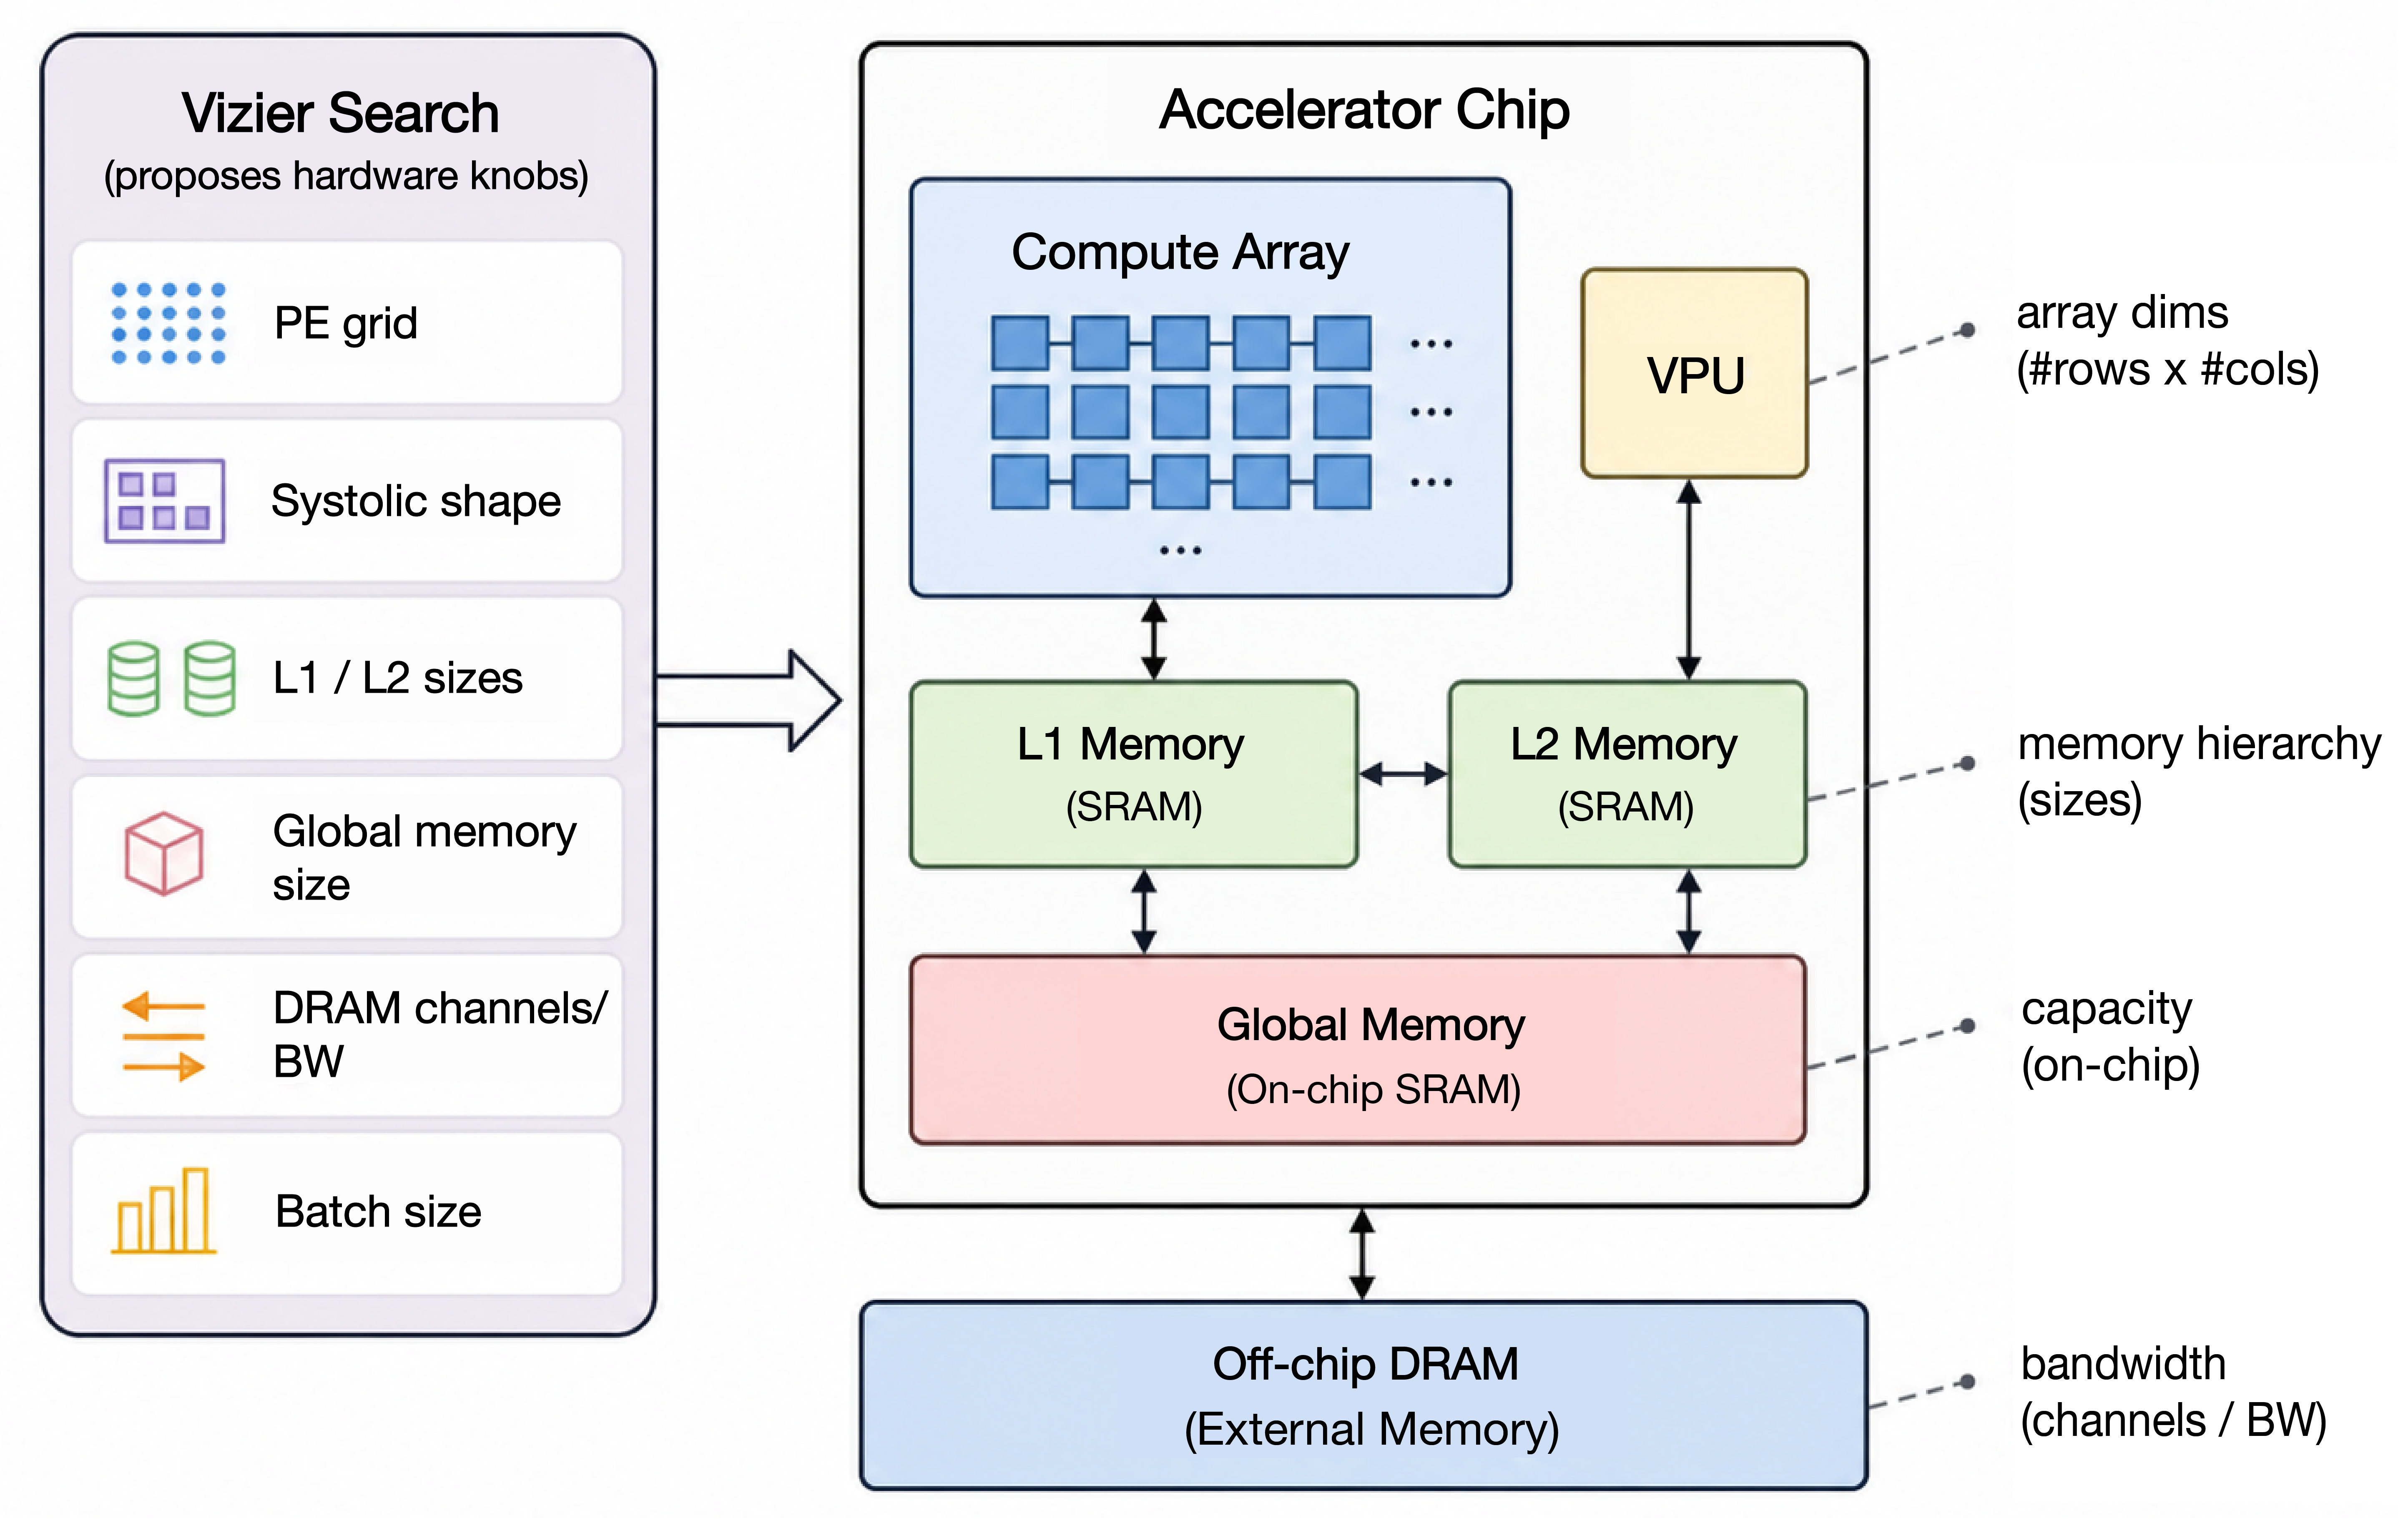
\includegraphics[width=0.7\linewidth]{figs/hardware_layout_v4.png}
%     \caption{The accelerator datapath configuration. Processing elements (PEs) are arranged in a grid connected by a mesh network. Each PE contains a systolic array for matrix operations, a vector processing unit (VPU) for non-MAC operations, and private or shared L1/L2 memory. A Global Memory serves as the on-chip scratchpad shared across all PEs.}
%     \label{fig:pipeline}
% \end{figure}
% \label{app:vizier}
% \begin{table}[h]
% \centering
% \caption{Vizier search parameter groups and ranges: initial small search vs.\ expanded V1-wide search.}
% \label{tab:vizier_search_space}
% \resizebox{\textwidth}{!}{%
% \begin{tabular}{llll}
% \toprule
% \textbf{Group} & \textbf{Parameter} & \textbf{Small (initial)} & \textbf{LLM-V1-wide} \\
% \midrule
% \multirow{16}{*}{\textbf{A — Hardware datapath (16 params)}}
%  & \texttt{PEs\_x\_dim}                & pow2 in $\mathbf{4 \ldots 32}$                          & pow2 in $\mathbf{1 \ldots 256}$                        \\
%  & \texttt{PEs\_y\_dim}                & pow2 in $\mathbf{4 \ldots 32}$                          & pow2 in $\mathbf{1 \ldots 256}$                        \\
%  & \texttt{Systolic\_array\_x}         & pow2 in $\mathbf{4 \ldots 32}$                          & pow2 in $\mathbf{4 \ldots 128}$                        \\
%  & \texttt{Systolic\_array\_y}         & pow2 in $\mathbf{4 \ldots 32}$                          & pow2 in $\mathbf{4 \ldots 128}$                        \\
%  & \texttt{Vector\_unit\_multiplier}   & pow2 $1 \ldots 16$                                      & pow2 $1 \ldots 16$                                     \\
%  & \texttt{L1\_buffer\_config}         & \{Private, Shared\}                                     & \{Private, Shared\}                                    \\
%  & \texttt{L1\_input\_buffer\_size}    & pow2 $\mathbf{1\,\text{KB} \ldots 4\,\text{MB}}$        & pow2 $\mathbf{1\,\text{KB} \ldots 1\,\text{MB}}$       \\
%  & \texttt{L1\_weight\_buffer\_size}   & pow2 $\mathbf{1\,\text{KB} \ldots 4\,\text{MB}}$        & pow2 $\mathbf{1\,\text{KB} \ldots 1\,\text{MB}}$       \\
%  & \texttt{L1\_output\_buffer\_size}   & pow2 $\mathbf{1\,\text{KB} \ldots 4\,\text{MB}}$        & pow2 $\mathbf{1\,\text{KB} \ldots 1\,\text{MB}}$       \\
%  & \texttt{L2\_buffer\_config}         & \{Disabled, Private, Shared\}                           & \{Disabled, Private, Shared\}                          \\
%  & \texttt{L2\_input\_buffer\_mult.}   & pow2 $1 \ldots 128$                                     & pow2 $1 \ldots 128$                                    \\
%  & \texttt{L2\_weight\_buffer\_mult.}  & pow2 $1 \ldots 128$                                     & pow2 $1 \ldots 128$                                    \\
%  & \texttt{L2\_output\_buffer\_mult.}  & pow2 $1 \ldots 128$                                     & pow2 $1 \ldots 128$                                    \\
%  & \texttt{L3\_global\_buffer} (CGM)   & $\{0\} \cup$ pow2 $\mathbf{1 \ldots 64\,\text{MB}}$     & $\{0\} \cup$ pow2 $\mathbf{1 \ldots 256\,\text{MB}}$   \\
%  & \texttt{GDDR6\_channels}            & pow2 $\mathbf{1 \ldots 16}$ ($\to$ 64–1024 GB/s)        & pow2 $\mathbf{1 \ldots 32}$ ($\to$ 64–2048 GB/s)       \\
%  & \texttt{Native\_batch\_size}        & pow2 $\mathbf{1 \ldots 1024}$                           & pow2 $\mathbf{1 \ldots 256}$                           \\
% \midrule
% \multirow{3}{*}{\textbf{B — Compiler passes (3 params)}}
%  & \texttt{two\_pass\_softmax}         & \{disabled, enabled\}                                   & \{disabled, enabled\}                                  \\
%  & \texttt{tensor\_padding}            & \{disabled, enabled\}                                   & \{disabled, enabled\}                                  \\
%  & \texttt{datatype}                   & \{bfloat16, int8\}                                      & \{bfloat16, int8\}                                     \\
% \midrule
% \multirow{2}{*}{\textbf{C — V0 rematerialisation (2 params)}}
%  & \texttt{remat\_enabled}             & \{disabled, enabled\}                                   & \{disabled, enabled\}                                  \\
%  & \texttt{remat\_cost\_scale}         & \{0.1, 0.25, 0.5, 1.0, 2.0, 4.0\}                      & \{0.1, 0.25, 0.5, 1.0, 2.0, 4.0\}                     \\
% \midrule
% \multirow{4}{*}{\textbf{D — V1 joint-tiling (4 params)}}
%  & \texttt{pareto\_config\_count\_C}   & \{10, 50, 100, 250, 500, 1000\}                         & \{10, 50, 100, 250, 500, 1000\}                        \\
%  & \texttt{loop\_ordering\_strategy}   & \{weight\_stationary, output\_stationary, both\}        & \{weight\_stationary, output\_stationary, both\}       \\
%  & \texttt{pareto\_pruning\_strategy}  & \{tmax\_workingset, tmax\_tmin, tmin\_workingset\}      & \{tmax\_workingset, tmax\_tmin, tmin\_workingset\}     \\
%  & \texttt{tile\_workingset\_modeling} & \{fixed, config\_dep\}                                  & \{fixed, config\_dep\}                                 \\
% \midrule
% \multirow{4}{*}{\textbf{Post-Vizier gates (filter, not search)}}
%  & \texttt{MIN\_TOTAL\_MACS}           & \multicolumn{2}{l}{$32{,}768$ ($4{\times}4{\times}4{\times}4{=}256$ lower physical, 32K gate)} \\
%  & \texttt{MAX\_TOTAL\_MACS} cap       & none — implicit $\leq 32{\times}32{\times}32{\times}32 \approx 1\,\text{M}$ & $1{,}048{,}576$ explicit cap \\
%  & Implied total\_MACs reach           & ${\approx}\,256 \ldots 1\,\text{M}$                     & $256 \ldots 1{,}048{,}576$ (post-cap)                  \\
%  & Implied DRAM BW reach               & $64 \ldots 1{,}024$ GB/s                                & $64 \ldots 2{,}048$ GB/s                               \\
% \bottomrule
% \end{tabular}%
% }
% \end{table}


\subsection{Why We Are Confident in the Software Side}
\label{app:sw_confidence}

The software claim is that the schedule the program commits to is the schedule
that runs, and that its optimality is bounded rather than asserted. Five
independent checks support it, ordered from strongest to weakest.

\paragraph{The committed schedule executes byte-exactly in RTL.}
The original DeepSeek-V3 validation schedule is compiled into a
$1{,}383$-instruction event tape
and executed on a cycle-accurate SystemVerilog engine under Verilator
(\cref{sec:rtl_validation}). The run completes with \textbf{zero} capacity
violations; the RTL peak on-chip occupancy equals the analytical prediction
\emph{exactly} at $7{,}602{,}176$~bytes; and the total cycle count lands within
$+0.000001\%$ of the rounded LP objective. This is the strongest form of the
claim available without silicon: the plan is not merely feasible on paper, it is
executable byte-for-byte on hardware that enforces the capacity constraint at
every step of that tape. This is not an RTL execution of the later
61,985,244-invocation native workload.

\paragraph{The checker is live, not vacuous.}
A validation suite is only meaningful if it can fail. We therefore replay a
deliberately over-committed tape, and the capacity checker flags exactly one
violation. A test that never fails proves nothing; this one fails when it should.

\paragraph{Optimality is bounded, not claimed.}
An admitted integral execution supplies a feasible endpoint under its modeled
contract. A lower bound applies only to the domain covered by its certificate;
working-support bounds cannot be promoted to the full library. The current
finite native family has a $21.6374\%$ continuous interval
(Appendix~\ref{app:native_provenance}). That interval is separate from the
recovered chip's predicted latency and is not a performance error bar.

\paragraph{Rounding is feasibility-preserving and independently validated.}
In the original campaign, relaxed selectors are rounded by enumeration over the physically integral
choices, and no pin that would violate a constraint is ever committed. Each
rounded design is re-solved and checked against the constraint set independently
of the solver that produced it, with residuals at the $10^{-13}$ level. We never
report a relaxed objective as an achievable result.

\paragraph{Search configurations remain explicit.}
The original campaign uses the configuration in
\cref{app:coeff_provenance}. The native extension separately records its
reference, recovered design, and matched controls in
Appendix~\ref{app:native_provenance}. Those controls share a chip and evaluator;
they are not globally optimized feature-off designs.

\paragraph{What this does not establish.}
RTL cycle counts are not used as an absolute oracle: the analytical per-layer
cache floors are conservative by $192\times$ to $2475\times$, so RTL evidence is
scoped to schedule realizability, memory legality, and utilization
\emph{mechanisms}. We make no claim that the simulated datapath is a
performance-optimal implementation.

\subsection{Why We Are Confident in the Hardware Side}
\label{app:hw_confidence}

The hardware evidence supports the declared cost-model mechanisms; it is not a
fabrication certificate for every modeled design. Design-space-exploration frameworks are conventionally validated
three ways, against measured taped-out chips, against post-synthesis extraction,
and against other frameworks~\citep{mei2021zigzag}. We have all three.

\paragraph{Against post-synthesis extraction: the area coefficient and its
functional form.}
We implement the scored datapath as synthesizable RTL and push it through
OpenROAD to placement at the ASAP7 $7$~nm predictive PDK
(\cref{sec:asap7}). Extracted cell area fits
$A = 82.08\,\mathrm{MACs} - 206.5\ \mu\mathrm{m}^2$ with $R^2 = 0.999999$, and
area per MAC varies by only $0.46\%$ across a $16\times$ range in MAC count. The
second number matters more than the first: the program assumes area is
\emph{linear with a size-independent slope}, and that is exactly what a placed
datapath exhibits. The coefficient we use is bracketed from below by extracted
cell area and from above by our own conservative floorplan.

\paragraph{Against shipped silicon: the energy coefficient.}
Our compute-energy coefficient corresponds to $0.40$~pJ per INT8 operation. Whole
chip figures for shipped accelerators are $0.35$ (H100), $0.64$ (A100) and
$1.27$~pJ/op (TPU-v4i), and an array-only coefficient must sit at or just below
whole-chip values. It does. We additionally measured the precision-energy ratio
directly rather than assuming it, and the measurement corrected our analytic
estimate in both directions (\cref{sec:energy_coeff}).

\paragraph{Against other frameworks: the mapping data.}
The original campaign's mapping data comes from Timeloop Pareto evaluations.
The native extension uses explicit analytical dispatch, primitive-service,
and memory-transfer contracts, as documented in
Appendix~\ref{app:native_provenance}.

\paragraph{Declared feasibility is checked.}
The original campaign enforces its six proxy gates. The native extension
checks its original LP rows, installed bank and staging resources, and
complete execution accounting. These are different evidence scopes; neither
replaces detailed physical implementation.

\paragraph{What this does not establish.}
We have not taped out, and we do not run clock-tree synthesis or routing, so we
make no claim about achievable clock frequency in silicon. Absolute power from
our own flow remains an upper bound rather than a prediction: an ungated tile
driven by uncorrelated data on a predictive PDK reports roughly three times our
coefficient, and we therefore anchor the coefficient to measured silicon rather
than to our own synthesis. The gating measurement in particular is not yet
trustworthy and no clock-gating decision is scored in the program as a result.

\clearpage
\newpage
\section{Speedup Analysis: Baseline Deficit Attribution and Design-Parameter Sensitivity}
\label{app:deficit}

A large end-to-end speedup number is only credible if two things are shown
explicitly: (i) the naive baseline actually \emph{carries} that deficit, and
the deficit can be \emph{localized} to a physical cause; and (ii) the reported
gain can be \emph{decomposed} into a small number of design decisions, each of
which is separately sized. This appendix supplies both. We first attribute the
naive-baseline per-operation runtime into compute-active versus memory-stall
(versus communication) time (\cref{app:deficit:perop}); we then decompose the
$34.6$--$40.2\times$ co-design speedup into exactly two orthogonal factors
(\cref{app:deficit:twofactor}); we sweep each design decision one at a time and
report the objective's sensitivity (\cref{app:deficit:sweeps}); and we rank the
decisions by objective sensitivity to guide where a chip designer should spend area
and power (\cref{app:deficit:ranking}). This section is a companion to the
pre-RTL feasibility gates of \cref{app:details}: the gates certify that a design
is \emph{buildable}; this section certifies where its speedup \emph{comes from}.

\paragraph{Reading conventions (read before any number below).}
Throughout, every quantity written \textbf{MFU} in this appendix is the
\textbf{compute-floor tightness} ratio
$\rho_{\mathrm{comp}}=t_{\mathrm{floor}}/T_{\mathrm{LP}}$ of \cref{app:mfu}
(the mapper-derived compute floor over the LP/analytic latency within one
cost-model convention). It is \emph{not} model-FLOP utilization in the sense of
\cref{sec:reported_quantities}, because its numerator is a Timeloop tile
minimum carrying the reference geometry's padding rather than a useful-work
count, and it is \emph{never} a measured-silicon utilization; the searched
datapaths are hypothetical, not fabricated. \textbf{Same-silicon} comparisons
are equal-area and equal-TDP \emph{by construction} (both sides share the PE
grid, so the area/power model of \cref{app:gates} returns identical budgets).
The $97\%$ pre-fusion memory-stall figures and the naive MFU values are
\emph{naive-baseline attributions}, not properties of the co-designed schedule.
Every quantity is convention-tagged, and we never form a ratio across two
conventions. The fixed-silicon algorithmic gain on EfficientNet-B7 is
$2.21\times$ under this paper's naive convention (a $2.81\times$ value that
appears in an earlier discussion note is a transcription error and is not used).

% ---------------------------------------------------------------------------
\subsection{Per-Operation Deficit Attribution}
\label{app:deficit:perop}

To justify a custom-silicon speedup on the order of $34$--$40\times$ we must
first show that the naive baseline wastes that much time, and say \emph{where}.
We attribute the naive per-operation runtime into three buckets:
\emph{compute-active} (the systolic array is issuing useful MACs),
\emph{memory-stall} (the array is idle waiting on off-chip traffic), and, for
multi-device / mixture-of-experts execution, \emph{communication} (inter-device
transfer of dispatched tokens or expert activations). On a single package the
communication bucket is empty by construction: all eight blueprints of
\cref{app:blueprints} hold their active working set on-package (for DeepSeek-V3,
the active-expert set is resident and the routing layer, not the datapath,
pages the full model), so no operation incurs cross-device traffic.

\paragraph{The deficit is memory stall, not communication.}
Two independent attributions, on two different silicon points, agree that the
naive deficit is almost entirely memory stall.

\emph{(a) On the co-designed chip (blueprint convention).} Before fusion and
time-indexed placement, naive per-operation streaming (each operation reads
all of its tensors from DRAM and writes them back) leaves the array stalled
on memory for $\mathbf{97.1}$--$\mathbf{97.5\%}$ of naive time
(\cref{tab:deficit_perop}; individual blueprints report $97.1\%$ for
Llama-1 13B/65B, $97.2\%$ for DeepSeek-V3, $97.5\%$ for Llama-3 70B). This is
large precisely because the co-designed chip provisions $20$--$27\times$ more
MACs than TPU-v3: the compute floor shrinks, so any unfused, re-streaming
schedule becomes memory-bound. Fusion plus time-indexed residency keep the
reused tensors on-chip and recover the schedule to the compute floor,
$\mathrm{MFU}=1.000$ (0.998 on Llama-1 13B; \cref{tab:cheetah_v1_llama1_13b}).

\emph{(b) On fixed TPU-v3 silicon (grid convention).} On the $65{,}536$-MAC
baseline itself, naive streaming reaches only $\mathrm{MFU}=0.40$--$0.64$ of the
compute floor on TPU-v3 (Llama-3 70B $0.399$, DeepSeek-V3 $0.451$,
Llama-1 13B $0.467$, SD1.5-UNet $0.643$), and up to $0.78$ across the
compute-bound cells of the wider fixed-hardware grid; on the bandwidth-starved
NPU ($64$\,GB/s) it collapses to $\mathrm{MFU}=0.02$--$0.05$. The joint schedule
recovers every compute-bound cell to $\mathrm{MFU}\approx1.000$, so the
fixed-silicon speedup is a \emph{pure utilization recovery}, not additional
compute.

\begin{table}[ht!]
\centering
\caption{Naive-baseline deficit attribution. Compute-active and memory-stall
fractions are $\mathrm{MFU}_{\mathrm{naive}}$ and $1-\mathrm{MFU}_{\mathrm{naive}}$
on fixed TPU-v3 silicon (grid convention, scale-$T_{\max}$ naive). Pre-fusion
memory stall is the blueprint-chip convention (naive per-op streaming on the
co-designed datapath). Communication is zero on a single package. The last
column is the joint schedule's recovered model-MFU. All values are
naive-baseline attributions under one cost-model convention (\cref{app:mfu});
they are not measured-silicon utilizations.}
\label{tab:deficit_perop}
\small
\begin{tabular}{@{}lccccc@{}}
\toprule
& \multicolumn{3}{c}{\textbf{Naive baseline (TPU-v3, per-op)}}
& \textbf{Pre-fusion stall} & \textbf{Joint} \\
\cmidrule(lr){2-4}
\textbf{Workload} & Compute-active & Memory-stall & Comm.\ & (chip, no fusion)
& $\mathrm{MFU}$ \\
\midrule
Llama-1 13B  & 0.467 & 0.533 & 0 & 97.1\% & 1.000 \\
Llama-1 65B  & --\,$^{\dagger}$ & --\,$^{\dagger}$ & 0 & 97.1\% & 1.000 \\
Llama-3 70B  & 0.399 & 0.601 & 0 & 97.5\% & 1.000 \\
DeepSeek-V3  & 0.451 & 0.549 & 0 & 97.2\% & 1.000 \\
SD1.5-UNet   & 0.643 & 0.357 & 0 & --      & 0.963 \\
\bottomrule
\end{tabular}

\vspace{2pt}
{\footnotesize $^{\dagger}$Llama-1 65B is not one of the five workloads in the
fixed-hardware MFU grid; its pre-fusion stall is read from
\cref{tab:cheetah_v1_llama1_65b}. Across the compute-bound cells of the wider
grid, naive MFU spans $0.40$--$0.78$; the bandwidth-starved NPU cells sit at
$0.02$--$0.05$.}
\end{table}

\paragraph{The stalled time is avoidable, not compulsory.}
The $97\%$ stall is \emph{re-streaming} of tensors that could have stayed
on-chip, not irreducible DRAM traffic. Two floor analyses bound the compulsory
component. First, on each blueprint the memory floor (compulsory bytes over the
chip's own bandwidth) is only $0.10$--$0.33\%$ of the compute floor
(Llama-1 13B $2.27\times10^{7}/2.31\times10^{10}=0.10\%$; Llama-3 70B $0.31\%$;
DeepSeek-V3 $0.33\%$; \cref{app:blueprints}). Second, a mapping-independent
attainable-traffic analysis in the style of Orojenesis~\citep{huang2024mindthegap}
places the attainable per-Einsum DRAM floor at $\mathbf{0.1}$--$\mathbf{0.9\%}$
of the compute floor on every cell we measured (Llama-3 70B $0.116\%$,
DeepSeek-V3 $0.182\%$, SD1.5-UNet $0.896\%$), because at the deployed
prefill-like batch the weight reuse is large. Both bound the same conclusion:
the compulsory off-chip traffic that \emph{no} schedule can remove is under
$1\%$ of the compute floor, so essentially the entire naive memory-stall
deficit is recoverable by scheduling (fusion, time-indexed residency, and
tile choice) and the recoverable ceiling is not gated by DRAM bandwidth or
by network communication.

\paragraph{Planned figure: per-operation stacked time breakdown.}
We will add a per-operation stacked-bar figure (one bar per HLO operation,
ordered by graph position; each bar split into compute-active / memory-stall /
communication seconds) for the naive baseline and for the CHEETAH schedule side
by side, on all four LLM blueprints, in the style of the FAST per-layer
utilization plot~\citep{zhang_fast} and Eyeriss-style per-layer accounting
\citep{chen2019eyerissv2flexibleaccelerator}. The naive bars are dominated by
the memory-stall segment ($\sim97\%$ aggregate); the CHEETAH bars are almost
pure compute-active (aggregate $\mathrm{MFU}\to1$); the communication segment is
empty on a single package and appears only in the multi-device / MoE variant of
\cref{app:deficit:sweeps}. This figure is a \emph{planned appendix experiment}
(the underlying per-op compute/stall decomposition exists in the solver output;
the figure is not yet rendered).
% TODO(figure): render figs/deficit_perop_stack.pdf from the per-op
% compute/stall/comm segments; naive vs CHEETAH, four LLM blueprints.

% ---------------------------------------------------------------------------
\subsection{Two-Factor Speedup Decomposition}
\label{app:deficit:twofactor}

The headline speedup factors \emph{exactly} into two orthogonal terms:
\begin{equation}
\underbrace{\frac{T_{\mathrm{naive}}(\text{TPU-v3})}{T_{\mathrm{joint}}(\text{chip})}}_{\text{headline}}
\;=\;
\underbrace{\frac{T_{\mathrm{naive}}(\text{TPU-v3})}{T_{\mathrm{joint}}(\text{TPU-v3})}}_{f_1:\ \text{scheduling recovery}}
\;\times\;
\underbrace{\frac{T_{\mathrm{joint}}(\text{TPU-v3})}{T_{\mathrm{joint}}(\text{chip})}}_{f_2:\ \text{MAC provisioning}} .
\label{eq:twofactor}
\end{equation}
The first factor $f_1$ is a \emph{fixed-silicon}, same-area / same-TDP
algorithmic gain: it re-schedules the same $65{,}536$-MAC TPU-v3 and buys
$\mathbf{1.48}$--$\mathbf{1.78\times}$. The second factor $f_2$ holds the joint
schedule fixed and provisions the PE grid up to the co-designed chip's MAC
count, buying $\mathbf{20.0}$--$\mathbf{26.9\times}$. Their product reproduces
the per-workload Figure-2 headline (and the blueprint ``achieved speedup vs.\
naive TPU-v3'' rows) to within $1.4\%$
(\cref{tab:deficit_twofactor}); the residual is the analytic
chip-endpoint solve's utilization roll-off, cross-checked against the
blueprints' Timeloop-in-loop objective.

\begin{table}[ht!]
\centering
\caption{Two-factor decomposition of the co-design speedup
(\cref{eq:twofactor}). $f_1$ is the fixed-silicon scheduling gain on TPU-v3
(same area/TDP), $f_2$ the MAC-provisioning gain to the co-designed chip.
Reconstructed $=f_1\times f_2$; headline is the blueprint value. Convention:
config-0 naive; bf16 cycle basis; HiGHS-Optimal endpoints.}
\label{tab:deficit_twofactor}
\small
\begin{tabular}{@{}lccccc@{}}
\toprule
\textbf{Workload} & $f_1$ (sched., TPU-v3) & $f_2$ (MAC prov.)
& Reconstructed & Headline & Recon./Headline \\
\midrule
Llama-1 13B  & 1.662 & 20.31 & 33.75 & 34.22 & 0.986 \\
Llama-1 65B  & 1.727 & 20.04 & 34.60 & 34.60 & 1.000$^{\ddagger}$ \\
Llama-3 70B  & 1.484 & 26.85 & 39.84 & 40.16 & 0.992 \\
DeepSeek-V3  & 1.784 & 19.97 & 35.63 & 35.68 & 0.999 \\
\midrule
\textbf{Range} & \textbf{1.48--1.78} & \textbf{20.0--26.9}
& \multicolumn{3}{c}{\textbf{34.6--40.2} (matches Fig.~2)} \\
\bottomrule
\end{tabular}

\vspace{2pt}
{\footnotesize $^{\ddagger}$Llama-1 65B's analytic chip-endpoint solve was
degenerate under HiGHS time limits, so its $f_2$ uses the authoritative
blueprint objective (exact by construction); the other three use the
\emph{independent} analytic chip solve and land within $1.4\%$.}
\end{table}

\paragraph{Is the provisioning factor physically usable?}
A reader is entitled to ask whether $f_2$ is real parallelism or an artifact of
a cost model in which compute time falls as $1/\mathrm{MACs}$ without bound. It
is a fair question: an array can only speed an operation up as far as that
operation supplies independent tiles to fill it, and a per-token decode GEMV
supplies few. We measured the answer directly rather than argue it. For every
event of DeepSeek-V3 we computed the \emph{saturating} MAC count
$M_{\mathrm{sat}} = (\text{independent output tiles}) \times (\text{lanes per
tile})$ under the same tile geometry the mapper uses, where independent tiles
are row tiles times column tiles (k-tiles accumulate into one output and are
not independent) times the number of GEMMs carrying work (expected active
experts for routed FFNs). Beyond $M_{\mathrm{sat}}$ a chip has no more
concurrent tiles to run for that event, and its compute time cannot keep
falling. \Cref{tab:msat} gives the distribution in multiples of the TPU-v3
array.

\begin{table}[ht!]
\centering
\small
\caption{Saturating MAC count per event, DeepSeek-V3, as a multiple of
TPU-v3's $65{,}536$ MACs. Prefill events saturate three to four orders of
magnitude above the largest chip in this paper ($24.4\times$), so the
provisioning factor $f_2$ is physically usable parallelism at prefill. Decode
events saturate at $9$--$14\times$ at the low end, which is where a bound on
usable parallelism would bind, and only for chips beyond it.}
\label{tab:msat}
\begin{tabular}{@{}llrrr@{}}
\toprule
Regime & Phase & min & p10 & median \\
\midrule
$B{=}8$, ctx $4096$   & prefill & $3{,}584\times$  & $3{,}584\times$  & $16{,}384\times$ \\
                      & decode  & $9\times$        & $14\times$       & $16\times$ \\
$B{=}32$, ctx $4096$  & prefill & $14{,}336\times$ & $14{,}336\times$ & $65{,}536\times$ \\
                      & decode  & $14\times$       & $14\times$       & $32\times$ \\
$B{=}32$, ctx $512$   & prefill & $1{,}792\times$  & $1{,}792\times$  & $8{,}192\times$ \\
                      & decode  & $14\times$       & $14\times$       & $32\times$ \\
\bottomrule
\end{tabular}
\end{table}

At the original prefill operating point, the table's tile geometry supplies
many independent matrix tiles, so useful parallelism is less restrictive than
it is for small decode matrices. The bound becomes relevant when installed
arrays exceed the independent work available to an event. These counts describe
the mapper's geometry, not placed-array timing, and do not account for growing
non-matrix costs. The native full-inference model instead charges padded matrix
service and explicit vector, local, and external service for each implementation
(Section~\ref{sec:decode_decomp}); its results must be read under that contract.

\paragraph{Use only the two-factor form; do not multiply the full decision ladder.}
It is tempting to read the software-ablation ladder (tile, placement, remat,
datapath, datatype) as a chain of multiplicative factors and multiply them all.
That \emph{overshoots} the headline by $1.8$--$2.1\times$ (a mechanical product
of $70.7$--$73.2\times$ versus the $34$--$40\times$ headline), for two
convention reasons, neither of them physics:
\begin{enumerate}
\item \textbf{The INT8 throughput label double-counts.} The blueprint headline
$T_{\mathrm{joint}}$ is a \emph{bf16 cycle count} at the chip's MAC count; INT8
(W8A8) is carried as a throughput / power label (roughly half the area and power
per MAC), \emph{not} as a separate cycle factor. Multiplying an extra $2\times$
for INT8 into a cycle product is a double-count. Dropping it lands the mechanical
ladder at $35$--$37\times$, within $3$--$12\%$ of the headline.
\item \textbf{The software rows use a $\sim1.3\times$ smaller naive baseline}
(the scale-$T_{\max}$ naive) than the config-0 naive against which the headline
is measured, so the two families of factors are not on the same numerator.
\end{enumerate}
\Cref{eq:twofactor} is the form that reconciles \emph{exactly} because $f_1$ and
$f_2$ share a single naive numerator and a single cycle basis. As a naming
caution: the same fixed-silicon scheduling recovery is $1.48$--$1.78\times$
against the config-0 naive (used above) and $2.14$--$2.51\times$ against the
grid's scale-$T_{\max}$ naive (the fixed-hardware grid convention of
\cref{app:deficit:perop}); the two differ only by the naive-baseline
definition, and must never be crossed within one ratio.

\paragraph{The provisioning factor is sub-linear (the anti-``just add MACs''
result).} $f_2$ is not free scaling. Measured as delivered throughput per
provisioned MAC in an equal-area / equal-TDP resource-matched ablation,
$20.0$--$27.0\times$ more MACs realize only $\approx16\times$ provisioning
throughput, a linearity of $\mathbf{0.59}$--$\mathbf{0.81}$ (Llama-3 70B is
worst, $27\times$ MACs $\to$ $16.0\times$). Equivalently, the fixed-family MAC
leg from $65{,}536$ to $1{,}048{,}576$ MACs (a $16\times$ increase) yields only
$14.0$--$15.7\times$ cycle reduction, because a residual memory floor remains.
Added silicon buys sub-linearly, which is exactly why capturing the free
scheduling factor $f_1$ first (and provisioning MACs only up to the point of
diminishing return) is the efficient order of operations.

% ---------------------------------------------------------------------------
\subsection{One-Decision-at-a-Time Sensitivity Sweeps}
\label{app:deficit:sweeps}

We now hold the design fixed and sweep a single decision, reporting the objective
(LP cycles) sensitivity. Two decisions have dedicated measured sweeps (global
buffer, MAC count); the remaining fine-grained sweeps (per-unit peak-FLOPS,
interconnect radix / link count) are framed here and marked as
\textcolor{orange!85!black}{\textbf{planned}} appendix experiments so they can be
added to the paper's experiment list; we do not fabricate their numbers.

\paragraph{(a) Global-buffer size $C_{\mathrm{GM}}$: measured, near-inert in
the compute-bound regime.} \Cref{tab:deficit_cgm} sweeps $C_{\mathrm{GM}}$ from
$1$ to $64$\,MiB for DeepSeek-V3 on TPU-v3 ($900$\,GB/s), for the joint (free-$y$)
LP and for a fixed-tile FAST-subset LP. The joint LP is \emph{flat}: its objective
moves $0.39\%$ across a $64\times$ buffer sweep ($1.0723\times10^{12}\to
1.0682\times10^{12}$ cycles), and is bit-identical from $8$\,MiB upward. By
contrast the fixed-tile schedule \emph{needs} the buffer, improving $1.18\times$
over the same sweep. The joint formulation substitutes tile choice for buffer
capacity: when tiling is free, a larger global buffer buys almost nothing. The
tile-dependent capacity extension is likewise inert here: it matches the retained joint model
to within $0.077\%$ across the full $C_{\mathrm{GM}}\in\{4,\dots,64\}$\,MiB sweep.
Under bandwidth pressure ($64$--$128$\,GB/s) the buffer regains a modest decision
($\approx1.19\times$ for Llama-1 13B over $8\to64$\,MiB), but \emph{only through
placement}: with placement frozen (row A) the objective is constant across
$C_{\mathrm{GM}}$, so $C_{\mathrm{GM}}$ helps exclusively by enabling
time-indexed residency, never on its own. The blueprints adopt
$C_{\mathrm{GM}}=64$\,MiB.

\begin{table}[ht!]
\centering
\caption{Global-buffer sweep, DeepSeek-V3 on TPU-v3 ($900$\,GB/s, native cache
convention, HiGHS-Optimal). The joint (free-$y$) LP is essentially
$C_{\mathrm{GM}}$-insensitive ($0.39\%$ over a $64\times$ sweep); the fixed-tile
FAST-subset LP is not ($1.18\times$). Objective in LP cycles.}
\label{tab:deficit_cgm}
\small
\resizebox{\linewidth}{!}{%
\begin{tabular}{@{}lcccccccc@{}}
\toprule
$C_{\mathrm{GM}}$ (MiB) & 1 & 2 & 4 & 8 & 16 & 32 & 64 & sweep ($1\!\to\!64$) \\
\midrule
Joint (free-$y$) & 1.0723 & 1.0699 & 1.0690 & 1.0682 & 1.0682
& 1.0682 & 1.0682 & $\times10^{12}$; $1.004\times$ \\
Fixed-tile (FAST-subset)   & 1.4627 & 1.4459 & 1.4327 & 1.4161 & 1.3863
& 1.3364 & 1.2371 & $\times10^{12}$; $1.182\times$ \\
\bottomrule
\end{tabular}%
}
\end{table}

\paragraph{(b) Peak throughput / MAC-unit count: measured (count), planned
(per-unit rate).} The total-MAC provisioning sweep is measured: raising the PE
grid from $65{,}536$ to $1{,}048{,}576$ MACs (a $16\times$ increase) reduces the
objective by $14.0$--$15.7\times$ (Llama-1 13B $15.72\times$, DeepSeek-V3
$14.98\times$, Llama-3 70B $14.04\times$, Llama-1 65B $14.02\times$), and the
provisioning factor to the full co-designed chip is $f_2=20.0$--$26.9\times$
(\cref{app:deficit:twofactor}), both sub-linear (\S\ref{app:deficit:twofactor}).
This is the single largest decision on the objective. A \emph{finer} sensitivity
that varies per-unit peak throughput (systolic-array dimensions, vector-lane
width, or clock) at a \emph{fixed} MAC count and fixed area, separating
``more units'' from ``faster units'', is not yet run and is marked
\textcolor{orange!85!black}{\textbf{planned}}; the datapath template of
\cref{app:gates} and MAGNet-style generators~\citep{venkatesan2019magnet}
already parameterize it.

\paragraph{(c) DRAM bandwidth: measured, inert in the compute-bound regime.}
Sweeping bandwidth from $900$ to $3{,}350$\,GB/s at the fixed $65{,}536$-MAC
point moves the objective by $\le0.25\%$ (BW leg $=1.000$--$1.0025\times$ for
all four LLMs): at the deployed prefill-like batch these workloads are
compute-bound, so bandwidth beyond the floor buys nothing. Bandwidth becomes the
dominant decision only in the bandwidth-starved regime: at $64$\,GB/s (the compact
NPU) the joint-vs-naive fixed-hardware gain is $5.9$--$31.4\times$, because there
the roofline is memory-bound and residency / placement recover a much larger
share. Thus bandwidth sensitivity is regime-dependent: near-zero when
compute-bound, first-order when memory-bound.

\paragraph{(d) Interconnect: on-chip NoC and inter-device topology (planned).}
Two interconnect decisions are framed but not yet swept.
\emph{On-chip}, the NoC / crossbar radix and link count set the PE-to-SRAM
routing capacity; this is the resource bounded by the crossbar / NoC-routing
gate of \cref{app:gates} (gate 4, $N_{\mathrm{NoC}}=n_{\mathrm{PEs}}\times
n_{\mathrm{banks}}\le5\times10^{6}$ cells), and its provisioning follows the
network-on-package accounting of Simba~\citep{shao2019simba}. In the single-chip
compute-bound regime the on-chip NoC is provisioned to the compute floor and is
not the binding resource, but a dedicated radix / link sweep (objective
versus NoC cells at fixed MACs) is
\textcolor{orange!85!black}{\textbf{planned}}.
\emph{Across devices}, in the multi-GPU / mixture-of-experts regime the
inter-device topology (radix and link count of the NVLink-class fabric) binds
only when experts are dispatched \emph{across} devices; when the active-expert
set is package-resident (as in every blueprint here) the communication term is
zero (\cref{app:deficit:perop}). A distributed / MoE topology sweep (objective
and the communication bucket versus inter-GPU radix and link count, in the
spirit of Chiplet-Cloud and wafer-scale serving
analyses~\citep{peng2024chipletcloudbuildingai,zhu2024theseusexploringefficientwaferscale}
and co-optimized network provisioning~\citep{rashidi2023unico}) is
\textcolor{orange!85!black}{\textbf{planned}}.

\begin{table}[ht!]
\centering
\caption{Single-decision sensitivity summary (compute-bound LLM regime, TPU-v3
operating point). ``Objective sensitivity'' is the LP-cycle response to the
stated sweep. Cells marked \textcolor{orange!85!black}{\textbf{planned}} have no
dedicated run yet and are listed as appendix experiments; their numbers are not
fabricated.}
\label{tab:deficit_sweepsummary}
\small
\begin{tabularx}{\linewidth}{@{}p{.20\linewidth}p{.25\linewidth}Xl@{}}
\toprule
\textbf{Decision} & \textbf{Sweep} & \textbf{Objective sensitivity} & \textbf{Status} \\
\midrule
Global buffer $C_{\mathrm{GM}}$ & $1\to64$\,MiB (BW$=900$)
& $1.004\times$ (joint); $1.18\times$ (fixed-tile) & measured \\
& under BW pressure ($\le128$) & $\approx1.19\times$, via placement only & measured \\
MAC count (total) & $65{,}536\to1{,}048{,}576$ ($16\times$)
& $14.0$--$15.7\times$ (sub-linear); $f_2=20.0$--$26.9\times$ & measured \\
Peak rate / unit & systolic dims, clock @ fixed MACs
& -- & \textcolor{orange!85!black}{\textbf{planned}} \\
DRAM bandwidth & $900\to3{,}350$\,GB/s & $\le1.003\times$ (compute-bound) & measured \\
& $64$\,GB/s (NPU) & $5.9$--$31.4\times$ (memory-bound) & measured \\
On-chip NoC radix / links & $N_{\mathrm{NoC}}$ at fixed MACs
& -- (gate 4 bounds it) & \textcolor{orange!85!black}{\textbf{planned}} \\
Inter-device topology (MoE) & inter-GPU radix / links
& -- (binds on cross-device dispatch) & \textcolor{orange!85!black}{\textbf{planned}} \\
\bottomrule
\end{tabularx}
\end{table}

% ---------------------------------------------------------------------------
\subsection{Decision-Impact Ranking}
\label{app:deficit:ranking}

\Cref{tab:deficit_ranking} ranks the decisions by objective sensitivity in the
compute-bound LLM regime and states \emph{why} each sits where it does, so a
chip designer can read off where area and power are best spent.

\begin{table}[ht!]
\centering
\caption{Design decisions ranked by objective sensitivity in the compute-bound LLM
regime (TPU-v3 operating point). ``Cost'' is what the decision spends on the die.
The ranking inverts in the memory-bound / distributed regimes, as noted.}
\label{tab:deficit_ranking}
\small
\begin{tabularx}{\linewidth}{@{}cp{.22\linewidth}p{.23\linewidth}p{.13\linewidth}X@{}}
\toprule
\textbf{Rank} & \textbf{Decision} & \textbf{Sensitivity} & \textbf{Cost}
& \textbf{Binds when} \\
\midrule
1 & MAC-count provisioning & $20.0$--$26.9\times$ (sub-linear) & area $+$ power
& always (compute-bound); diminishing returns \\
2 & Scheduling (tile+fusion+placement) & $1.48$--$1.78\times$ & none (same silicon)
& always; also a feasibility enabler at tight buffers \\
3 & DRAM bandwidth & $\approx1.0\times$; $5.9$--$31.4\times$ if starved & pins $+$ power
& memory-bound regime only \\
4 & Global buffer $C_{\mathrm{GM}}$ & $\approx1.0\times$; $\le1.19\times$ pressed & area (SRAM)
& buffer-pressed regime; only via placement \\
5 & Interconnect (NoC / inter-GPU) & $\approx1.0\times$ on-chip & area $+$ links
& distributed / MoE cross-device dispatch \\
\bottomrule
\end{tabularx}
\end{table}

\paragraph{Why this ordering, and what it tells a designer.}
In the compute-bound LLM regime the objective is set by how many useful MACs the
schedule can keep busy. \textbf{(1) MAC-count provisioning} moves the objective
most ($20$--$27\times$) but sub-linearly and at direct area/power cost, so it is
the decision to spend on, up to the point of diminishing return, and never past
the feasibility gates of \cref{app:gates} (a bigger matrix unit can even degrade
delivered performance, as observed for production TPU
silicon~\citep{jouppi2017datacenter}). \textbf{(2) Scheduling} is a
\emph{free} multiplier ($1.48$--$1.78\times$ at equal area and TDP) that must be
captured first: it costs no silicon, it is what recovers naive MFU $0.40$ to
$\approx1.0$, and at tight buffers it is a feasibility enabler, not merely an
optimization (on EfficientNet-B7 at TPU-v3's $32$\,MiB buffer the pure-streaming
row is infeasible and time-indexed placement restores feasibility: placement
alone at $2.03\times$, joint optimum $2.21\times$). \textbf{(3) DRAM bandwidth} and \textbf{(4) global buffer} are
near-inert once compute-bound (bandwidth beyond the floor and buffer beyond a
few MiB buy essentially nothing; \cref{tab:deficit_cgm}), and the joint LP
actively trades buffer for tile choice, so paying for HBM or a large global SRAM
buys lower TDP-per-TFLOP, not more throughput, at these operating points. Both
become first-order only when the workload is genuinely memory-bound (low
bandwidth, or decode-time batch-1 operational intensity). \textbf{(5)
Interconnect} is inert on a single compute-bound chip and matters only in the
distributed / MoE regime, when experts are dispatched across devices and the
communication bucket becomes nonzero. The practical guidance: \emph{buy MACs
(watching the sub-linear roll-off and the gates), capture scheduling for free,
and invest in bandwidth, buffer, or interconnect only when the regime (memory-
or communication-bound) actually makes them bind.}

\paragraph{Sweeps requiring new runs (for the paper's experiment list).}
The following are framed above but not yet run, and are proposed as appendix
experiments: (i) a per-unit peak-throughput sweep (systolic dimensions / clock
at fixed MAC count and area), isolating ``faster units'' from ``more units'';
(ii) an on-chip NoC radix / link-count sweep (objective versus $N_{\mathrm{NoC}}$
at fixed MACs, tied to gate 4); (iii) an inter-device / MoE topology sweep
(objective and the communication bucket versus inter-GPU radix and link count,
with experts dispatched across devices); and (iv) the per-operation stacked
compute/stall/communication time-breakdown figure of \cref{app:deficit:perop}.

\clearpage
\newpage
\section{Qualitative Design Discussion}
\label{app:solver}

Wall-clock time decomposition and search acceleration results are presented in Figure~\ref{fig:wallclock} and Section~\ref{sec:experiments}.


\subsection{Interesting Empirical Design Results}

\begin{table}[ht!]
\centering
\caption{Surprise design pairs discovered by CHEETAH. Each pair achieves near-identical Perf/TDP via qualitatively different strategies that are not intuitive to human engineers.}
\label{tab:surprise_designs}
\resizebox{\textwidth}{!}{%
\begin{tabular}{llrrrrrrrrr}
\toprule
\textbf{Label} & \textbf{Workload} & \textbf{Trial} &
\textbf{Perf/TDP $\times$} & \textbf{Speedup $\times$} &
\textbf{MACs} & \textbf{CGM} &
\textbf{L1 in/w/o (KB)} & \textbf{L1 cfg} &
\textbf{L2 cfg} & \textbf{Batch} \\
\midrule
TPU-v3 ref   & --              & --  & 1.000 & 1.000  & 65{,}536  & 32 MB & 64 / 64 / 64     & Shared  & Disabled & 64  \\
\midrule
DeepSeek A   & \texttt{deepseek\_v3} & 81 & 3.158 & 25.125 & 524{,}288 & 8 MB  & 512 / 1 / 256    & Shared  & Disabled & 64  \\
DeepSeek B   & \texttt{deepseek\_v3} & 95 & 3.146 & 12.512 & 262{,}144 & 8 MB  & 1 / 256 / 512    & Shared  & Disabled & 128 \\
\midrule
Llama-3 70B A & \texttt{llama3\_70b} & 88 & 3.557 & 14.152 & 262{,}144 & 32 MB & 8 / 256 / 4      & Private & Shared   & 64  \\
Llama-3 70B B & \texttt{llama3\_70b} & 92 & 3.570 & 28.402 & 524{,}288 &  1 MB & 512 / 128 / 512  & Shared  & Shared   & 64  \\
\bottomrule
\end{tabular}%
}
\end{table}

We examine two designs on the DeepSeek-V3  (trials 81 vs.\ 95) and Llama-3 70B (trials 88 vs.\ 92) workloads. In each case, Perf/TDP scores are nearly identical yet design specifications are hugely different. DeekSeek's Design B uses 262K MACs vs.\ 524K in Design A. B compensates via richer search and larger batch. Pareto-tile space is 50$\times$ larger in B (500 vs.\ 10 configs); batch size doubles (128 vs.\ 64). Mirror-image L1 sub-buffer allocation in A keeps 512 KB input + 1 KB weight + 256 KB output. Design B keeps 1 KB input + 256 KB weight + 512 KB output. These two entirely opposite on-chip memory strategies yield identical system efficiency. On Llama-3 70B pair (trials 88 vs.\ 92), design A uses 262K MACs and 32 MB Global Buffer; Design B uses 524K MACs and only 1 MB Global Buffer. However Design A is weight-stationary, with a large 256 KB weight L1, tiny 8/4 KB input/output L1, and weight reuse amortised over a large on-chip scratchpad. Whereas Design B is activation-stationary, with 512/512 KB input/output L1, only 128 KB weight L1, and shared L1 configuration seen in doubled MACs allow CGM to collapse to 1 MB. This provides insight that additional compute in B substitutes for global memory capacity: higher throughput reduces the time activations must remain resident, relaxing the CGM capacity constraint. 


\subsection{Hardware and Vizier Search}

In all experiments, we utilize 16 NVIDIA H100 GPUs. Each unit in the configuration provides 80 GB of VRAM, totaling 1.28 TB of available memory across the cluster. The system is characterized by a high memory bandwidth of approximately 3.35 TB/s per GPU, which is critical for the memory-intensive workloads examined in this work. In order to be consistent with prior work on accelerator design \citep{zhang_fast}, we utilize Vizier to simulate TPUv3 and perform hardware search. \cref{tab:vizier_search_space} presents Vizier's search parameter groups for completeness, and \cref{fig:pipeline} depicts standard accelerator datapath configuration layout. 

A Processing Element (PE) is a repeated compute tile in an accelerator template.
The datapath can be modeled as a grid of PEs connected by a mesh on-chip network.
PE systolic arrays perform a matrix-vector multiply each cycle. 
Vector and scalar MACs are modeled by setting systolic array X and Y dimensions to 1. 
PEs also contain a VPU for non-MAC vector ops. 
L2 and Global Memory structures are optional. 

\begin{figure}[ht!]
    \centering
    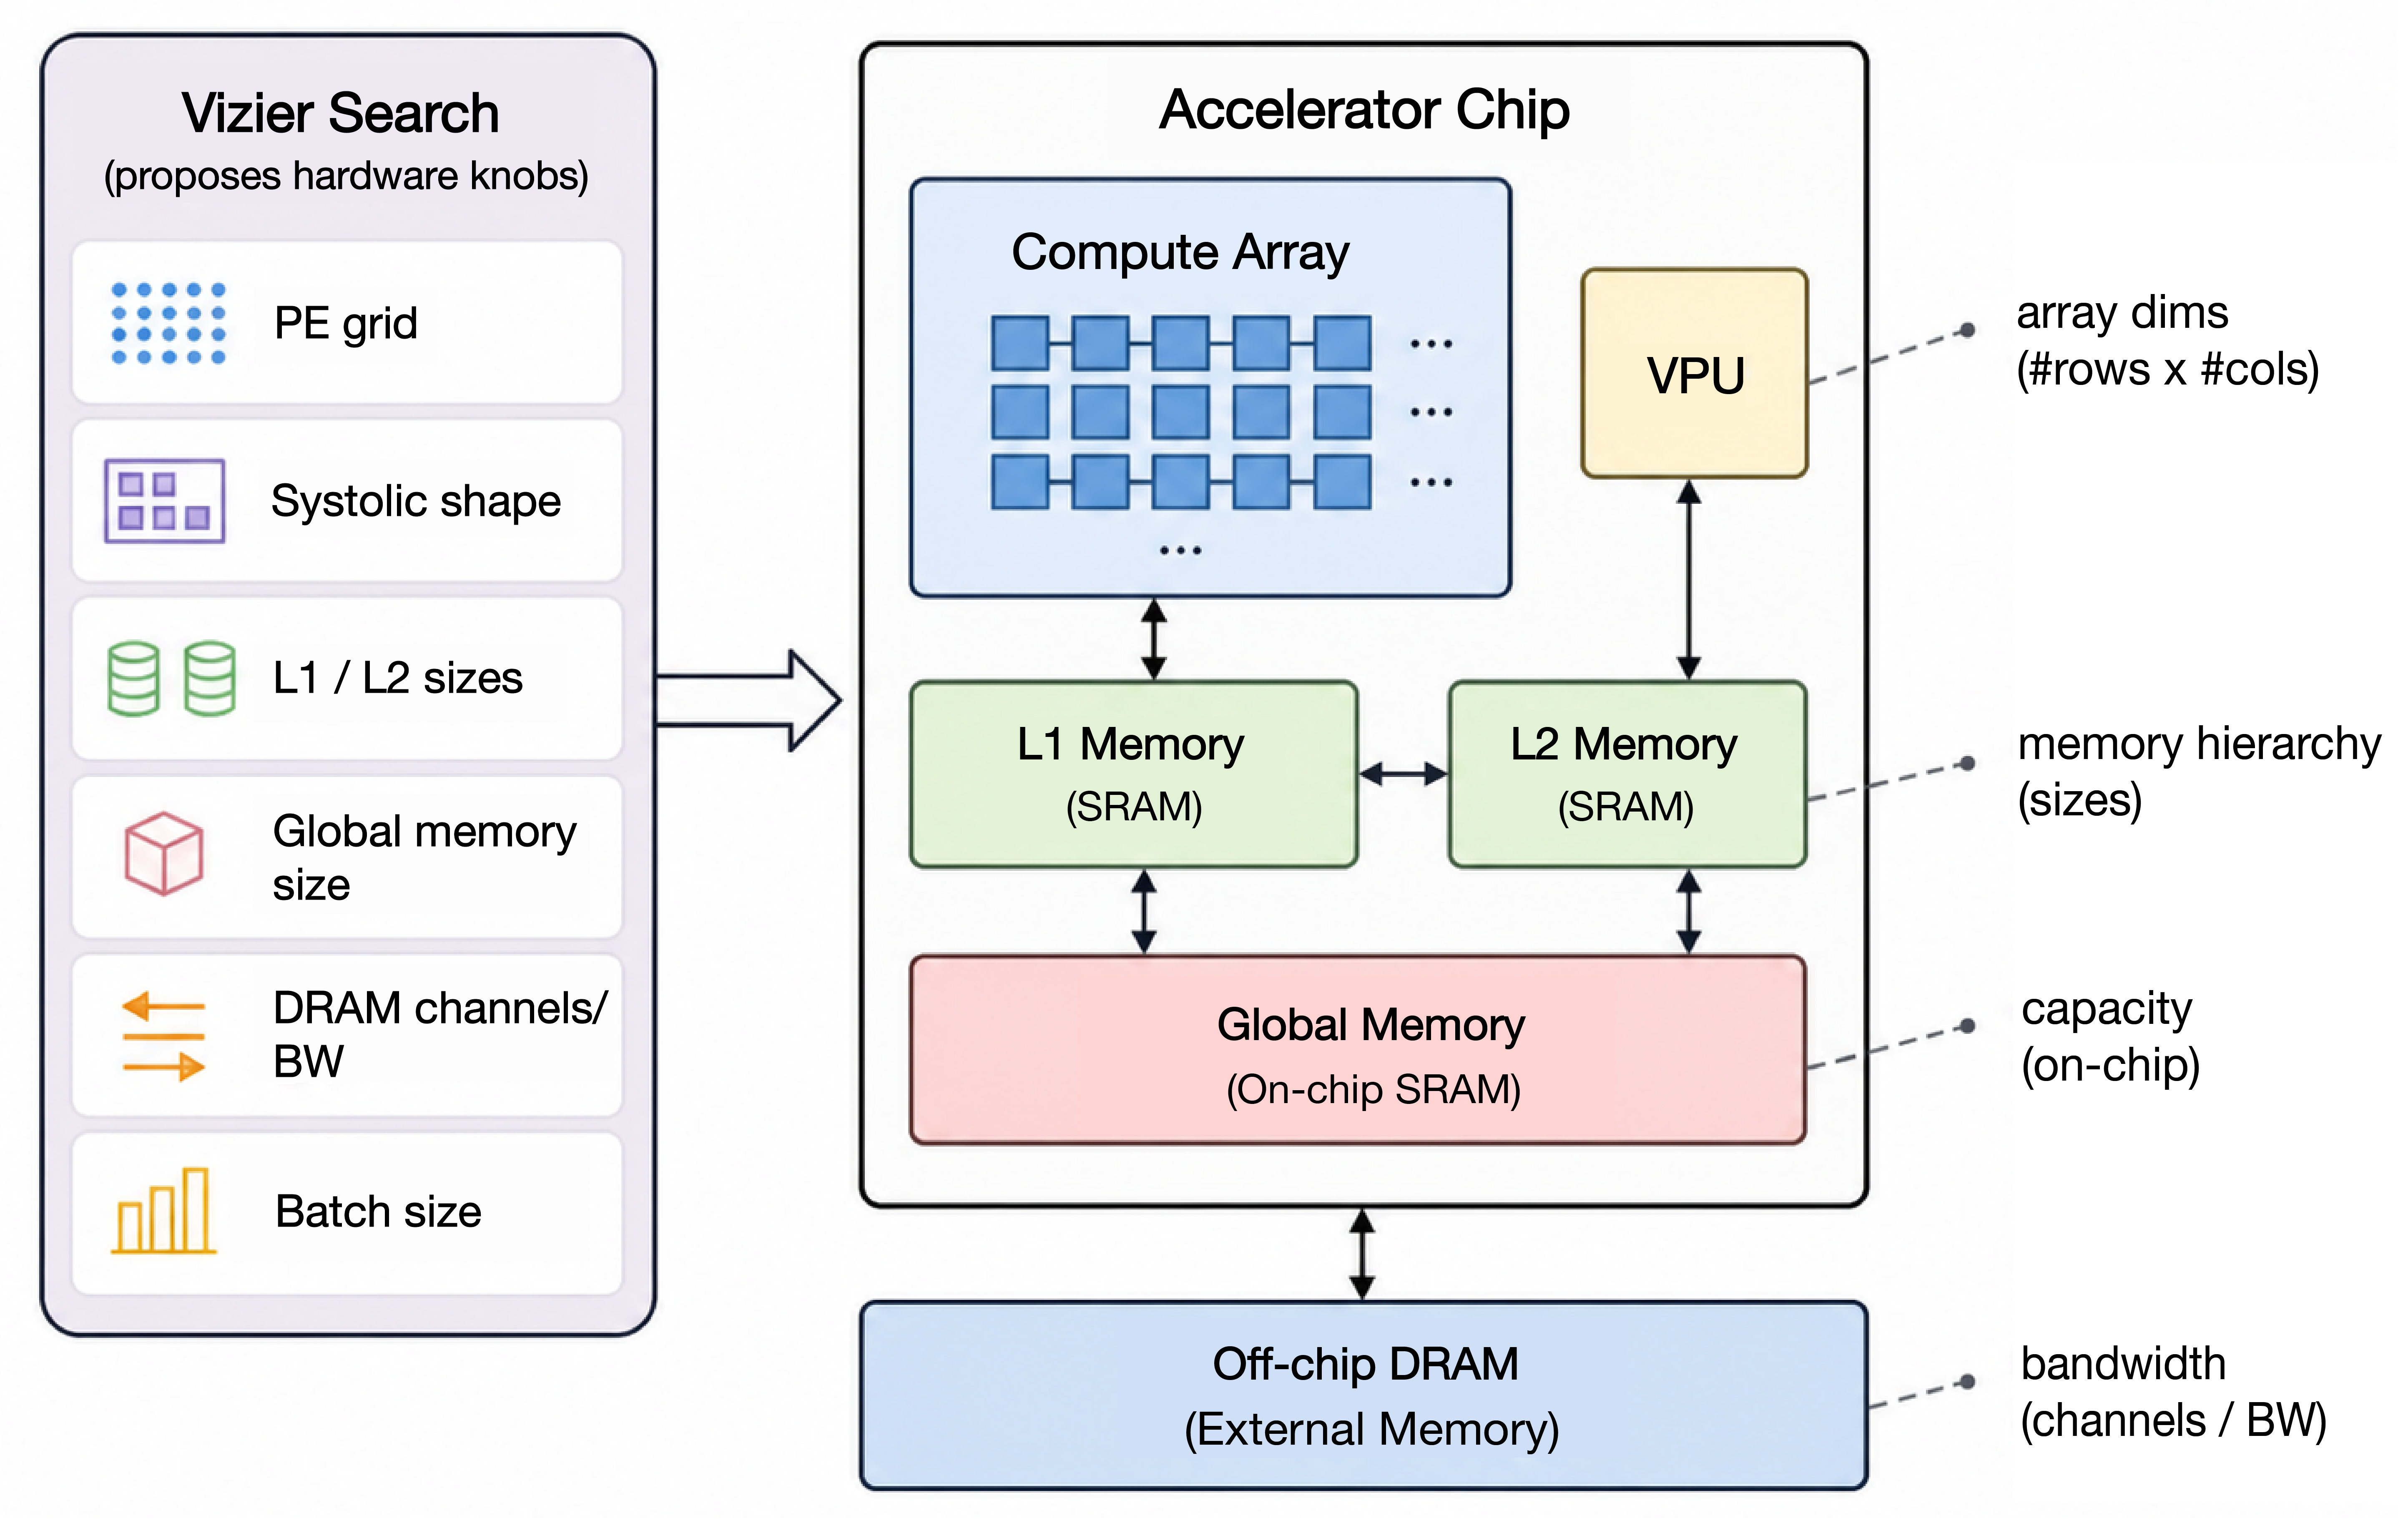
\includegraphics[width=0.7\linewidth]{figs/hardware_layout_v4.png}
    \caption{The accelerator datapath configuration. Processing elements (PEs) are arranged in a grid connected by a mesh network. Each PE contains a systolic array for matrix operations, a vector processing unit (VPU) for non-MAC operations, and private or shared L1/L2 memory. A Global Memory serves as the on-chip scratchpad shared across all PEs.}
    \label{fig:pipeline}
\end{figure}
\label{app:vizier}


\begin{table}[h]
\centering
\caption{Vizier search parameter groups and ranges: initial small search vs.\ expanded joint-tile-wide search.}
\label{tab:vizier_search_space}
\resizebox{\textwidth}{!}{%
\begin{tabular}{llll}
\toprule
\textbf{Group} & \textbf{Parameter} & \textbf{Small (initial)} & \textbf{LLM-joint-tile-wide} \\
\midrule
\multirow{16}{*}{\textbf{A: Hardware datapath (16 params)}}
 & \texttt{PEs\_x\_dim}                & pow2 in $\mathbf{4 \ldots 32}$                          & pow2 in $\mathbf{1 \ldots 256}$                        \\
 & \texttt{PEs\_y\_dim}                & pow2 in $\mathbf{4 \ldots 32}$                          & pow2 in $\mathbf{1 \ldots 256}$                        \\
 & \texttt{Systolic\_array\_x}         & pow2 in $\mathbf{4 \ldots 32}$                          & pow2 in $\mathbf{4 \ldots 128}$                        \\
 & \texttt{Systolic\_array\_y}         & pow2 in $\mathbf{4 \ldots 32}$                          & pow2 in $\mathbf{4 \ldots 128}$                        \\
 & \texttt{Vector\_unit\_multiplier}   & pow2 $1 \ldots 16$                                      & pow2 $1 \ldots 16$                                     \\
 & \texttt{L1\_buffer\_config}         & \{Private, Shared\}                                     & \{Private, Shared\}                                    \\
 & \texttt{L1\_input\_buffer\_size}    & pow2 $\mathbf{1\,\text{KB} \ldots 4\,\text{MB}}$        & pow2 $\mathbf{1\,\text{KB} \ldots 1\,\text{MB}}$       \\
 & \texttt{L1\_weight\_buffer\_size}   & pow2 $\mathbf{1\,\text{KB} \ldots 4\,\text{MB}}$        & pow2 $\mathbf{1\,\text{KB} \ldots 1\,\text{MB}}$       \\
 & \texttt{L1\_output\_buffer\_size}   & pow2 $\mathbf{1\,\text{KB} \ldots 4\,\text{MB}}$        & pow2 $\mathbf{1\,\text{KB} \ldots 1\,\text{MB}}$       \\
 & \texttt{L2\_buffer\_config}         & \{Disabled, Private, Shared\}                           & \{Disabled, Private, Shared\}                          \\
 & \texttt{L2\_input\_buffer\_mult.}   & pow2 $1 \ldots 128$                                     & pow2 $1 \ldots 128$                                    \\
 & \texttt{L2\_weight\_buffer\_mult.}  & pow2 $1 \ldots 128$                                     & pow2 $1 \ldots 128$                                    \\
 & \texttt{L2\_output\_buffer\_mult.}  & pow2 $1 \ldots 128$                                     & pow2 $1 \ldots 128$                                    \\
 & \texttt{L3\_global\_buffer} (CGM)   & $\{0\} \cup$ pow2 $\mathbf{1 \ldots 64\,\text{MB}}$     & $\{0\} \cup$ pow2 $\mathbf{1 \ldots 256\,\text{MB}}$   \\
 & \texttt{GDDR6\_channels}            & pow2 $\mathbf{1 \ldots 16}$ ($\to$ 64–1024 GB/s)        & pow2 $\mathbf{1 \ldots 32}$ ($\to$ 64–2048 GB/s)       \\
 & \texttt{Native\_batch\_size}        & pow2 $\mathbf{1 \ldots 1024}$                           & pow2 $\mathbf{1 \ldots 256}$                           \\
\midrule
\multirow{3}{*}{\textbf{B: Compiler passes (3 params)}}
 & \texttt{two\_pass\_softmax}         & \{disabled, enabled\}                                   & \{disabled, enabled\}                                  \\
 & \texttt{tensor\_padding}            & \{disabled, enabled\}                                   & \{disabled, enabled\}                                  \\
 & \texttt{datatype}                   & \{bfloat16, int8\}                                      & \{bfloat16, int8\}                                     \\
\midrule
\multirow{2}{*}{\textbf{C: fixed-tile rematerialisation (2 params)}}
 & \texttt{remat\_enabled}             & \{disabled, enabled\}                                   & \{disabled, enabled\}                                  \\
 & \texttt{remat\_cost\_scale}         & \{0.1, 0.25, 0.5, 1.0, 2.0, 4.0\}                      & \{0.1, 0.25, 0.5, 1.0, 2.0, 4.0\}                     \\
\midrule
\multirow{4}{*}{\textbf{D: joint-tile joint-tiling (4 params)}}
 & \texttt{pareto\_config\_count\_C}   & \{10, 50, 100, 250, 500, 1000\}                         & \{10, 50, 100, 250, 500, 1000\}                        \\
 & \texttt{loop\_ordering\_strategy}   & \{weight\_stationary, output\_stationary, both\}        & \{weight\_stationary, output\_stationary, both\}       \\
 & \texttt{pareto\_pruning\_strategy}  & \{tmax\_workingset, tmax\_tmin, tmin\_workingset\}      & \{tmax\_workingset, tmax\_tmin, tmin\_workingset\}     \\
 & \texttt{tile\_workingset\_modeling} & \{fixed, config\_dep\}                                  & \{fixed, config\_dep\}                                 \\
\midrule
\multirow{4}{*}{\textbf{Post-Vizier gates (filter, not search)}}
 & \texttt{MIN\_TOTAL\_MACS}           & \multicolumn{2}{l}{$32{,}768$ ($4{\times}4{\times}4{\times}4{=}256$ lower physical, 32K gate)} \\
 & \texttt{MAX\_TOTAL\_MACS} cap       & none: implicit $\leq 32{\times}32{\times}32{\times}32 \approx 1\,\text{M}$ & $1{,}048{,}576$ explicit cap \\
 & Implied total\_MACs reach           & ${\approx}\,256 \ldots 1\,\text{M}$                     & $256 \ldots 1{,}048{,}576$ (post-cap)                  \\
 & Implied DRAM BW reach               & $64 \ldots 1{,}024$ GB/s                                & $64 \ldots 2{,}048$ GB/s                               \\
\bottomrule
\end{tabular}%
}
\end{table}
\clearpage
\newpage


\section{LLM-Architect Outer Loop Details}
\label{app:llm_loop}
The LLM-Architect outer loop proceeds through the following steps for each campaign round:

\begin{enumerate}

\item \textbf{Extraction.} Deterministic scripts summarize recent trials
into a \emph{Causal Ledger}. Each record includes hardware parameters,
validity, Perf/TDP, LP cycles, capacity duals/slacks, bandwidth
sensitivity, MFU, memory utilization, roofline gap, failure class, and LP solver metrics.

\item \textbf{Context building.} The last $N$ trials and the Causal Ledger
are compressed into a compact JSON context for the Strategist. The context
emphasizes empirical feasibility, observed invalid regions, best known
valid designs, and physical audit signals.

\item \textbf{Architect.} The online Architect, implemented as
Qwen2.5-7B-Instruct with a LoRA adapter trained on past trial logs, diagnoses the dominant bottleneck and emits a campaign patch. The patch constrains macro-architectural search decisions such as Global Memory, DRAM bandwidth, total MACs, systolic shape,
PE grid, and batch size. A larger teacher model, DeepSeek-V3.2, was used offline to generate or critique campaign labels, but is not in the live loop.

\item \textbf{Campaign validation.} A deterministic validator clips or rejects the LLM patch to enforce legal hardware ranges, TDP and area limits, MAC caps, CGM feasibility floors, compute/bandwidth coupling, and roofline constraints. This prevents the LLM from proposing physically implausible regions such as maximum-MAC/minimum-bandwidth designs. 

\item \textbf{Local optimization.} Vizier is initialized inside the
validated patch and warm-started with prior trials that lie in the same region. Vizier then samples concrete hardware candidates within the approved campaign. The LLM chooses the high-level architectural neighborhood, while Vizier performs local adaptive optimization.

\item \textbf{Unified joint-tile Formulation.} The large-scale LP solver evaluates each candidate by solving the joint-tile joint tiling-fusion-placement LP using saved Pareto $\mathcal{C}$-sets. It returns the objective, cycles, selected tiling configurations, placement/rematerialization decisions, dual/slack summaries, and solver-quality diagnostics.

\item \textbf{Roofline audit.} A deterministic Roofline Auditor checks whether the predicted latency is physically plausible. For each candidate,
we compute
\begin{align}
    t_{\text{compute}} &= \frac{\text{useful FLOPs}}{\text{peak FLOPs/s}},
    \qquad
    t_{\text{memory}}  = \frac{\text{post-placement DRAM bytes}}{\text{peak bandwidth}},
    \nonumber\\
    t_{\text{ideal}}   &= \max\!\left(t_{\text{compute}},\, t_{\text{memory}}\right).
\end{align}
A candidate is rejected if the solver-reported latency falls below this lower bound, or if MFU or memory utilization exceeds 1.0 within tolerance.

\item \textbf{Ledger update.} The loop records the campaign hypothesis, intervention, observed invalid-rate change, MFU change, roofline validity, and best Perf/TDP change. The ledger also records forbidden regions when a campaign produces excessive invalid trials.

\item \textbf{Shortlist Pareto refinement.} At the end of a campaign or study, only the top-ranked candidates are passed to a Pareto refinement run. This reruns targeted Timeloop refinement
for selected configurations and re-solves joint-tile LP, providing a final trust check. This is an additional and optional sanity check step.

\end{enumerate}

The Architect receives workload summaries, invalid-rate history, MFU, roofline signals, and prior valid regions, normalized LP duals and bandwidth sensitivities. The system starts from a safe empirically valid patch and allows duals only to make bounded edits, such as raising the CGM floor, increasing bandwidth, reducing MAC count, or changing systolic shapes. The validator rejects any dual-guided patch that excludes known high-performing valid regions or predicts a substantially worse feasible rate.


\subsection{Profile-Conditioned LLM-Architect Application}
\label{app:profiles}

We evaluate if the Architect can condition hardware search on deployment intent, since speech models may prioritize latency while data analytics models may prioritize bandwidth. For each workload, we run the same Qwen2.5-LoRA Strategist, validator, random-in-patch sampler, and joint-tile LP evaluator while changing only a two-paragraph profile block describing the user’s objective and constraints. The resulting best chips differ systematically by profile: overnight batch profiles select higher-bandwidth and larger-CGM regions, compact-edge profiles select smaller feasible regions with the lowest invalid rate, and interactive profiles favor small-CGM, extreme-aspect datapaths. Since the inner joint-tile LP and validator are identical across profiles, these differences isolate the effect of the LLM’s profile-conditioned search patch. The absolute Perf/TDP often remains within a narrow band because the joint-tile evaluator reaches a similar structural ceiling, but the hardware families used to reach that ceiling differ substantially. We simulate two user profiles: (1) interactive speech is a spoken dialogue model where latency is more important than bandwidth, and (2) overnight finance batch where the user requires a large amount of financial data to be processed, but might leave it overnight to complete hence bandwidth is more important than latency.

The LLM-Architect clearly learned the profile distinction. Different profiles select meaningfully different chips for the same workload. The signal flows through the LLM's patch choice (steered by the profile prompt), and random-in-patch sampling finds the best chip within each profile-narrowed region. Table~\ref{tab:profile_best_chips} gives examples of best designs per profile. 

\begin{table}[h]
\centering
\caption{Best hardware configuration discovered per (deployment profile,
workload) cell. PE\,SA = PE grid $\times$ systolic array dimensions.
MACs = total multiply-accumulate units. BW = DRAM bandwidth (GB/s).
CGM = Global Buffer size (MB). Interactive speech = small low-latency-style chip, overnight finance batch = high-throughput, high-bandwidth, compact edge = compact constrained chip, balanced cloud = moderate/general design.}
\label{tab:profile_best_chips}
\resizebox{\textwidth}{!}{%
\begin{tabular}{llllrrrr}
\toprule
\textbf{Workload} & \textbf{Profile} &
\textbf{PE grid} & \textbf{Systolic} &
\textbf{MACs} & \textbf{BW (GB/s)} &
\textbf{CGM (MB)} &
\textbf{Best Perf/TDP $\times$} \\
\midrule
\multirow{4}{*}{Llama-1 13B}
 & \texttt{interactive\_speech}      & $1\times128$ & $16\times16$  & 32K   & 512  & 2   & 2.06 \\
 & \texttt{overnight\_finance\_\allowbreak batch}& $16\times8$  & $128\times32$ & 524K  & 2048 & 256 & 2.73 \\
 & \texttt{compact\_edge}            & $8\times2$   & $64\times32$  & 32K   & 512  & 4   & 2.06 \\
 & \texttt{balanced\_cloud}          & $2\times256$ & $8\times16$   & 65K   & 64   & 128 & 2.97 \\
\midrule
\multirow{4}{*}{DeepSeek-V3}
 & \texttt{interactive\_speech}      & $1\times32$  & $8\times128$  & 32K   & 2048 & 16  & 1.07 \\
 & \texttt{overnight\_finance\_\allowbreak batch}& $8\times256$ & $16\times8$   & 262K  & 2048 & 1   & 2.55 \\
 & \texttt{compact\_edge}            & $16\times64$ & $16\times4$   & 65K   & 128  & 2   & 2.99 \\
 & \texttt{balanced\_cloud}          & $256\times2$ & $32\times16$  & 262K  & 1024 & 32  & 2.83 \\
\bottomrule
\end{tabular}%
}
\end{table}

\begin{itemize}[leftmargin=1.4em, itemsep=3pt]

    \item \textbf{\texttt{interactive\_speech}} repeatedly selects
          extreme-aspect PE arrays ($1{\times}32$, $1{\times}128$,
          $1{\times}256$, $2{\times}128$); these favour narrow systolic
          streaming for low single-batch latency. CGM is consistently
          small (2–4 MB), trading cache capacity for compute density.
          Matches the profile intent: ``minimize end-to-end latency,
          batch $\leq 8$''.

    \item \textbf{\texttt{overnight\_finance\_\allowbreak batch}} consistently
          selects high bandwidth (1024–2048 GB/s) and often large CGM
          (16–256 MB). Matches the profile intent: ``maximize throughput,
          large batch, sustained bandwidth''.

    \item \textbf{\texttt{compact\_edge}} consistently selects the
          smallest chips (32–65K MACs is common vs.\ 524K for other
          profiles) with tiny CGM (1–4 MB). Matches the profile
          hard constraints: TDP $\leq 0.5\times$, area $\leq 0.5\times$,
          mobile deployment target.

    \item \textbf{\texttt{balanced\_cloud}} selects medium-everything
          (middle-of-the-road MACs, bandwidth, and CGM), consistent
          with its unconstrained balanced objective.

\end{itemize}

\paragraph{Invalid-Rate Signal}

\begin{table}[h]
\centering
\caption{Average invalid rate per deployment profile. The LLM responds
to profile constraints: tighter profiles produce more LP-rejected
proposals, while compact profiles are more feasible despite strict
TDP/area limits.}
\label{tab:profile_invalid_rates}
\begin{tabularx}{\linewidth}{@{}p{.29\linewidth}lX@{}}
\toprule
\textbf{Profile} & \textbf{Avg.\ invalid rate} & \textbf{Interpretation} \\
\midrule
\texttt{interactive\_speech}       & 62\% &
Tightest profile (TDP $\leq 1\times$, batch $\leq 8$): LLM proposes
patches the LP frequently rejects. \\
\texttt{overnight\_finance\_\allowbreak batch} & 53\% &
Loose TDP ($4\times$) but \texttt{min\_batch} $\geq 32$ forces
large-batch hardware. \\
\texttt{compact\_edge}             &  8\% &
Despite strict TDP/area constraints, the LLM finds feasible compact
regions easily: best feasibility of all profiles. \\
\texttt{balanced\_cloud}           & 36\% &
Middle-ground constraints produce intermediate invalid rate. \\
\bottomrule
\end{tabularx}
\end{table}


The absolute Perf/TDP$\,\times$ values are similar within a workload
across profiles (e.g.\ Llama-3 70B: $3.38$–$3.53$ across all four
profiles, within ${\approx}5\%$). This is not a failure: it reflects the LP's structural ceiling at fixed compute. \emph{What differs is the chip family used to reach that ceiling.} This is precisely the design-space-narrowing benefit of profile conditioning: the same headline Perf/TDP number is achieved by hardware families with qualitatively different deployment characteristics (narrow streaming chips for interactive speech, large-bandwidth chips for overnight batch), demonstrating that profile conditioning the LLM-Architect steers the search toward different hardware trade-offs without sacrificing overall efficiency.



\subsection{LLM in the Loop Prompts}
\label{app:prompt}
\begin{tcolorbox}[
    colback=blue!4,
    colframe=blue!55,
    title=\textbf{The Strategist System Prompt},
    fonttitle=\bfseries,
    breakable,
    before upper={\setlength{\parskip}{4pt}},
    left=4pt, right=4pt, top=4pt, bottom=4pt
]

You are the Strategist agent in a hardware/software co-design loop.

Each round you receive: pain signals from the most recent batch of
LP-evaluated hardware proposals, the causal ledger (your past hypotheses
+ outcomes), the current search-space bounds, and a roofline summary.
You return \textbf{ONE JSON object} describing a campaign that narrows
the search space for the next round.

You are a \emph{campaign-level search-space editor}, not a performance
predictor. Your job is to point Vizier at a small, physically-plausible
neighborhood; the deterministic Validator + roofline auditor enforce hard
constraints.

\medskip
\textbf{Important facts about the evaluator (CORGIsolve joint-tile).}
For each fixed hardware candidate, joint-tile already \emph{jointly} optimizes:
\begin{itemize}[leftmargin=1.4em, itemsep=1pt, topsep=2pt]
    \item per-layer tiling selection $y_{i,c}$ over precomputed Pareto
          tiling sets $\mathcal{C}_i$
    \item time-indexed activation and weight placement
    \item rematerialization decisions
    \item tiling $\times$ placement interactions via McCormick variables
    \item fusion / DRAM-traffic reduction under the candidate's memory
          capacity
\end{itemize}

\noindent Therefore: do \textbf{not} assume low Perf/TDP is caused by a
missing tiling search. The inner LP is already choosing the best available
tiling/fusion/placement plan for the candidate. Your job is \textbf{only}
to edit the \emph{outer} hardware search region.

\medskip
\textbf{Pain signal keys.}
\begin{itemize}[leftmargin=1.4em, itemsep=1pt, topsep=2pt]
    \item \texttt{invalid\_rate}: fraction of round's trials not OK
    \item \texttt{mfu\_med}, \texttt{memory\_util\_med}: median compute / memory utilization ($\leq 1$)
    \item \texttt{gap\_to\_floor\_med}: median $t_{\mathrm{solver}} / t_{\mathrm{ideal}}$ ($\geq 1$; near-1 $=$ at floor)
    \item \texttt{op\_intensity\_med}: median FLOPs/byte for OK trials
    \item \texttt{ridgepoint\_med}: median chip ridgepoint (FLOPs/byte)
    \item \texttt{capacity\_dual\_p95}, \texttt{bandwidth\_dual\_p95}, \texttt{macfloor\_dual\_p95}: LP duals
    \item \texttt{best\_perf\_tdp\_so\_far}: running max Perf/TDP across the search
    \item \texttt{recent\_roofline}: \texttt{\{violation\_rate, dominant\_violation, \ldots\}}
\end{itemize}

\medskip
\textbf{Causal reading.}
\begin{enumerate}[leftmargin=1.6em, itemsep=2pt, topsep=2pt]
    \item \texttt{capacity\_dual} high \emph{or} failures are
          \texttt{global\_memory\_infeasible} $\Rightarrow$ increase CGM
          or restrict to configs with enough global memory. Do \textbf{not}
          blindly increase MACs.
    \item \texttt{memory\_util} high, \texttt{gap\_to\_floor} low, or
          \texttt{op\_intensity\_med} $<$ \texttt{ridgepoint\_med}
          $\Rightarrow$ increase bandwidth, \emph{reduce} MAC count, or
          avoid max-MAC/min-BW regions.
    \item MFU low \emph{and} \texttt{memory\_util} also low $\Rightarrow$
          compute shape / systolic mismatch. Prefer different-shaped
          systolic arrays, \textbf{not} more total MACs.
    \item Perf/TDP plateaued $\Rightarrow$ propose an
          \texttt{efficiency\_shrink} campaign that keeps $\geq 95\%$ of
          best Perf/TDP while reducing TDP / area / invalid rate.
    \item Previous campaign had \texttt{invalid\_rate} $> 50\%$
          $\Rightarrow$ do \textbf{not} repeat or further narrow into that
          region. Shift to the nearest empirically valid region.
    \item \emph{Empirical feasibility beats unverified dual reasoning.}
          Never choose a patch that excludes the best known valid
          configurations unless explicitly running a small \texttt{explore}
          campaign.
\end{enumerate}

\noindent\textbf{Duals are advisory, not absolute.} If dual-based
reasoning conflicts with empirical feasibility, prioritise empirical
feasibility.

\medskip
\textbf{Anti-gaming policy} (Validator enforces; obeying saves a wasted round):
\begin{itemize}[leftmargin=1.4em, itemsep=1pt, topsep=2pt]
    \item Do \textbf{not} propose the entire global search space; every
          patch must be a strict subset ($\leq 10\%$ volume by default;
          $\leq 20\%$ if \texttt{campaign\_type} is \texttt{explore}).
    \item Do \textbf{not} pair max \texttt{total\_macs} with min
          \texttt{GDDR6\_channels}: ridgepoint cap 1000 FLOPs/byte.
    \item Do \textbf{not} propose tiny CGM ($\leq 1$ MB) for LLM
          workloads. Long-context workloads need $\geq 16$ MB CGM
          ($\geq 32$ MB for 65B+).
    \item Do \textbf{not} re-propose regions marked forbidden in the
          ledger.
\end{itemize}

\medskip
\textbf{Patchable parameters} (each must remain a non-empty subset of
original powers-of-two):
\texttt{PEs\_x\_dim}, \texttt{PEs\_y\_dim}, \texttt{Systolic\_array\_x},
\texttt{Systolic\_array\_y}, \texttt{Vector\_unit\_multiplier},
\texttt{L1\_\{input,weight,output\}\_buffer\_size},
\texttt{L2\_\{input,weight,output\}\_buffer\_multiplier},
\texttt{L3\_global\_buffer\_size} (CGM in MB),
\texttt{GDDR6\_channels}, \texttt{Native\_batch\_size}.

\medskip
\textbf{Output:} one JSON object on one line. No prose, no markdown fence.

\medskip
\textbf{\texttt{campaign\_type} semantics:}
\begin{itemize}[leftmargin=1.4em, itemsep=1pt, topsep=2pt]
    \item \texttt{exploit}: narrow region around best valid designs so far
    \item \texttt{repair}: targeted intervention for the dominant bottleneck
    \item \texttt{explore}: diverse region not covered by prior failed
          campaigns (validator allows up to 20\% of global space)
    \item \texttt{efficiency\_shrink}: Perf/TDP saturated; find a
          \emph{smaller} chip that keeps $\geq 95\%$ of best Perf/TDP
          while reducing TDP / area / invalid rate
\end{itemize}

\noindent If no actionable hypothesis exists: return
\texttt{campaign\_name} = \texttt{"explore\_current"},
\texttt{campaign\_type} = \texttt{"explore"}, empty
\texttt{search\_patch}, \texttt{dominant\_bottleneck} =
\texttt{"invalidity"}, and reasonable prediction fields.

\end{tcolorbox}
\begin{tcolorbox}[
    colback=grey!4,
    colframe=grey!55,
    title=\textbf{Teacher/Critic System Prompt},
    fonttitle=\bfseries,
    breakable,
    before upper={\setlength{\parskip}{4pt}},
    left=4pt, right=4pt, top=4pt, bottom=4pt
]

You are the \textbf{teacher/critic} for a hardware/software co-design
search loop.

\medskip
\noindent You are given:
\begin{itemize}[leftmargin=1.4em, itemsep=1pt, topsep=2pt]
    \item a \emph{Trial Digest} (pain signals from a campaign round)
    \item a \emph{deterministic oracle patch} (search-space narrowing that
          empirically worked in the next round of a previous run)
    \item the student-style template
\end{itemize}

\noindent Your task is to produce a \textbf{cleaned training example}.
The patch and prediction \textbf{must} stay grounded in the deterministic
oracle: do \textbf{not} invent new bounds. You may:

\begin{itemize}[leftmargin=1.4em, itemsep=1pt, topsep=2pt]
    \item rewrite \texttt{causal\_hypothesis} to be precise and cite the
          dominant signal
    \item tighten \texttt{dominant\_bottleneck} to the right category
    \item quantify \texttt{prediction} deltas (e.g.\ ``drop below 0.25'',
          ``increase by 0.10'')
    \item normalize \texttt{campaign\_name} to \texttt{snake\_case}
    \item reject the example by returning
          \texttt{\{"keep": false, "reason": "..."\}} if the deterministic
          oracle is internally inconsistent or unsafe
\end{itemize}

\medskip
\noindent Return \textbf{one JSON object on one line}. Schema:

\medskip
\noindent\textbf{Accept:}
\begin{quote}
\small
\texttt{\{"keep": true, "campaign\_name": "...", "causal\_hypothesis":
"...", "dominant\_bottleneck":
"capacity|\allowbreak bandwidth|\allowbreak compute\_shape|\allowbreak tdp|\allowbreak invalidity|\allowbreak roofline\_violation",
"search\_patch": <unchanged from oracle>, "prediction":
\{...quantitative...\}\}}
\end{quote}

\noindent\textbf{Reject:}
\begin{quote}
\small
\texttt{\{"keep": false, "reason": "..."\}}
\end{quote}

\end{tcolorbox}



\begin{tcolorbox}[
    colback=green!6,
    colframe=green!45!black,
    title=\textbf{Deployment Profile: \texttt{interactive\_speech}},
    fonttitle=\bfseries,
    breakable,
    left=4pt, right=4pt, top=4pt, bottom=4pt
]
\begin{verbatim}
DEPLOYMENT PROFILE (active for this campaign)
  natural-language goal: Minimize end-to-end latency for streaming
                         speech inference. Throughput is secondary.
                         Power should stay moderate. Small batch sizes
                         only; single-request latency is the metric.
  objective_mode:        min_latency
  soft preferences:      prefer_batch_size=small,
                         prefer_latency=very_high,
                         prefer_throughput=medium,
                         prefer_bandwidth=medium,
                         prefer_area=medium
  hard constraints:      max_tdp_relative=1.0,
                         max_area_relative=1.0,
                         max_batch_size=8
  search hint (use as prior_centroid neighborhood):
    native_batch_size:       [1, 2, 4, 8]
    L3_global_buffer_size:   [16, 32, 64, 128]

Tailor `search_patch` to this profile. Do NOT always maximize
Perf/TDP; respect the profile's objective_mode. CORGIsolve V1
still optimizes inner-loop tiling/fusion/remat for each chip;
your job is to point it at the chip region whose trade-offs
match this user need.
\end{verbatim}
\end{tcolorbox}

\bigskip

\begin{tcolorbox}[
    colback=green!6,
    colframe=green!45!black,
    title=\textbf{Deployment Profile: \texttt{overnight\_finance\_\allowbreak batch}},
    fonttitle=\bfseries,
    breakable,
    left=4pt, right=4pt, top=4pt, bottom=4pt
]
\begin{verbatim}
DEPLOYMENT PROFILE (active for this campaign)
  natural-language goal: Maximize throughput for large overnight
                         historical-data analysis. Latency is not
                         important. Sustained throughput and memory
                         bandwidth matter most. TDP/power can be
                         high as long as the work completes by
                         deadline.
  objective_mode:        max_throughput_per_tdp
  soft preferences:      prefer_batch_size=large,
                         prefer_latency=low,
                         prefer_throughput=very_high,
                         prefer_bandwidth=very_high,
                         prefer_area=medium
  hard constraints:      max_tdp_relative=4.0,
                         min_batch_size=32
  search hint (use as prior_centroid neighborhood):
    native_batch_size:       [64, 128, 256]
    GDDR6_channels:          [16, 32]
    L3_global_buffer_size:   [128, 256]

Tailor `search_patch` to this profile. Do NOT always maximize
Perf/TDP; respect the profile's objective_mode. CORGIsolve V1
still optimizes inner-loop tiling/fusion/remat for each chip;
your job is to point it at the chip region whose trade-offs
match this user need.
\end{verbatim}
\end{tcolorbox}

\subsection{Resource Prices and Proposal Validation}\label{app:llm_duals}
Resource prices summarize the current identified program. Proposals can target
expensive service, workspace, or retention constraints, but must be checked
against their complete implementation contract. A proposal list is not an
exhaustive pricing oracle: exhausting that list cannot establish full-master
optimality. The native experiments use separately admitted schedules and
complete-domain bound arguments as described in Appendix~\ref{app:native_provenance}.

\clearpage
\section{Two Optimal Tiling Examples: joint-tile LP Solution at a Glance}
\label{app:tiling}
This section shows examples of optimal tiling, where accepting a locally slower/smaller tiling to enable better fusion or placement.
This showcases the strength of the CHEETAH formulation, which discovers nontrivial tiling-placement-fusion trade-offs that less expressive methods would miss. The first example is Llama-3 70B on a modeled H100; the second is DeepSeek-V3 on a modeled RTX~5090.

By fixing the architecture, the inner loop derives optimal tiling and scheduling strategies that can act as custom speedups for targeted inference tasks. Therefore this section briefly provides motivation for future work on expanded hardware variants. This is motivated and similar in spirit to the speedups seen be FlashAttention \citep{dao2022flashattention} due to tiling optimization. 

% \begin{table}[ht!]
% \centering
% \caption{Per-chip V1 LP scheduling lift over naive (greedy) scheduling
% on the same modelled hardware. Speedup $=$ \texttt{static.objective\_cycles}
% $\div$ \texttt{v1\_rounded.objective\_cycles}.
% Source: \texttt{exp3\_<hw>\_*.csv}.}
% \label{tab:v1_per_chip_lift}
% \small
% \begin{tabular}{@{}llr@{}}
% \toprule
% \textbf{Workload} & \textbf{Hardware} &
% \textbf{V1 LP speedup over naive} \\
% \midrule
% Llama-3 70B  & H100      & $3.06\times$ \\
% DeepSeek-V3  & RTX~5090  & $5.51\times$ \\
% \bottomrule
% \end{tabular}
% \end{table}

\subsection{joint-tile LP Solution: Llama-3 70B on modeled H100}

\noindent\textbf{Problem dimensions:}
$L = 720$ layers, $C = 20$ tile configs, $T = 720$ timesteps,
$E = 703$ activation edges.
Total LP variables: 1{,}601{,}280.
Objective: $542{,}790{,}817$ cycles.
\texttt{CONVERGED\_STRICT} in 1{,}800 PDLP iterations.

\paragraph{Tile-Config Selection ($y_{i,c}$):} The joint-tile LP heavily favours small/fast configurations. Table~\ref{tab:tile_band} groups tiles into three size bands, and Table~\ref{tab:config_histogram} gives the per-config histogram.

\begin{table}[h]
\centering
\caption{Tile-config band distribution across $L=720$ layers.}
\label{tab:tile_band}
\begin{tabular}{lrr}
\toprule
\textbf{Tile size band} & \textbf{Layers} & \textbf{\% of model} \\
\midrule
Small ($c = 0\ldots4$): fast / large working set  & 427 & 59\% \\
Medium ($c = 5\ldots14$)                            & 275 & 38\% \\
Large ($c = 15\ldots19$): slow / small working set &  18 &  2\% \\
\bottomrule
\end{tabular}
\end{table}

\noindent Config histogram (picks per config index):

\begin{table}[h]
\centering
\caption{Number of layers assigned to each tile config $c$.
Configs with zero picks are omitted.}
\label{tab:config_histogram}
\begin{tabular}{lrrrrrrrrrr}
\toprule
$c$ & 0 & 1 & 3 & 4 & 5 & 8 & 12 & 16 & 17 \\
\midrule
Layers & 285 & 1 & 1 & 140 & 1 & 148 & 125 & 15 & 3 \\
\bottomrule
\end{tabular}
\end{table}

\noindent Config $c=0$ (largest tile) was selected for ${\approx}40\%$
of layers, with $c \in \{4, 8, 12\}$ covering most of the remainder.
The LP decisively favours large tiles for this 70B model on H100:
with 1.05M MACs and a 50 MB global buffer, reducing tile size to fit
memory is unnecessary and incurs iteration overhead.

\paragraph{Per-Layer Execution Time $T_i$:}

\[
    T_i^{\min} = 1{,}204 \text{ cycles}, \quad
    T_i^{\mathrm{med}} = 524{,}288, \quad
    T_i^{\max} = 1{,}835{,}008, \quad
    \textstyle\sum T_i = 542{,}790{,}817.
\]

\noindent The ten longest layers (Table~\ref{tab:longest_layers}) all hit the same $1{,}835{,}008$-cycle bound: these are the large FFN gate/up/down and Q/K/V/output projection sublayers in the transformer middle blocks:

\begin{table}[h]
\centering
\caption{Ten longest layers. All hit the maximum $T_i =
1{,}835{,}008$ cycles and correspond to large FFN/attention
projection sublayers.}
\label{tab:longest_layers}
\begin{tabular}{rrl}
\toprule
\textbf{Layer idx} & \textbf{$T_i$ (cycles)} & \textbf{Selected config $c$} \\
\midrule
359 & 1{,}835{,}008 &  4 \\
376 & 1{,}835{,}008 &  4 \\
375 & 1{,}835{,}008 &  4 \\
368 & 1{,}835{,}008 &  4 \\
  0 & 1{,}835{,}008 &  4 \\
367 & 1{,}835{,}008 &  4 \\
718 & 1{,}835{,}008 &  0 \\
358 & 1{,}835{,}008 &  8 \\
357 & 1{,}835{,}008 &  8 \\
377 & 1{,}835{,}008 & 12 \\
\bottomrule
\end{tabular}
\end{table}

\paragraph{Placement ($p$, $p^W$): Global Buffer Residency}

\begin{itemize}[leftmargin=1.4em, itemsep=2pt]
    \item Activation edges pinned at $t=0$: $0\ /\ 703$
    \item Weight layers pinned at $t=0$: $0\ /\ 720$
    \item Total $p$-cells set across all $t$:
          $0\ /\ 506{,}160$ ($0.00\%$)
    \item Total $p^W$-cells set across all $t$:
          $1\ /\ 518{,}400$ ($0.00\%$)
\end{itemize}

\noindent The joint-tile LP makes almost no use of the global buffer for
long-lived tensor residency and nearly everything streams through.
With the L1/L2 buffer multipliers in this hardware configuration,
\textbf{tiling alone is sufficient to keep the chip fed}; persistent pins are not needed.

\paragraph{Rematerialization Events $r_{i,t}$}

\[
    \text{Layers with} \geq 1\ \text{remat event}: 0\ /\ 720.
    \qquad
    \text{Total remat events}: 0.
\]

\noindent Zero Rematerialization. joint-tile has the freedom to recompute
layers to free memory pressure, but on this cell determined it was
not worth the additional cycles. Activation streaming combined with
tile-config selection is sufficient.

\paragraph{Eviction / Restoration Timeline}

\begin{itemize}[leftmargin=1.4em, itemsep=2pt]
    \item Activation evictions / restorations: $0\ /\ 0$
    \item Weight evictions / restorations: $1\ /\ 1$
          (one weight churn across all 720 timesteps)
\end{itemize}

\paragraph{One Concrete Layer: Layer 360 (Deep Transformer Block)}

\[
    \text{Selected config}\ c = 0, \qquad T_i = 524{,}288\ \text{cycles}.
\]
\[
    \mathbf{y}_{\mathrm{bin}}\ \text{nonzero indices}: \{0,\ 16\}
\]
The LP relaxation assigned nonzero weight to two equally-good configs

\paragraph{What This Reveals About joint-tile on Llama-3 70B / H100}

\begin{enumerate}

    \item \textbf{Tile choice does most of the work, not placement or remat.} Of 1.6M decision variables, only ${\approx}720$
          (the $y_{i,c}$ selections) are doing real work; placement
          ($p$, $p^W$) and rematerialisation ($r$) variables are
          essentially all zero.

    \item \textbf{Large tiles win because H100 is large.} With
          1.05M MACs and 3.35 TB/s DRAM bandwidth, there is no memory
          slack pressure forcing small working sets. The LP exploits
          this by selecting the largest physically permissible tiles.

    \item \textbf{The $1.53\times$ lift over the naive baseline comes
          entirely from per-layer tile selection.} Ten different configs
          are active across the 720 layers, versus the naive
          one-size-fits-all heuristic. On smaller chips (e.g.\ TPU-v3)
          this same mechanism yields a $2.11\times$ lift, because the
          memory slack disappears and per-layer tile choice becomes
          correspondingly more impactful.

\end{enumerate}


% As a qualitative example of V1’s solution structure, we inspect the rounded V1 LP solution for DeepSeek-V3 on an RTX-5090-like hardware point. The model contains L=903 layers, including 174 MoE sublayers, and the V1 LP has 2.5M variables. Although the Pareto cache exposes 20 tile configurations per layer, the solution uses only five configs, {0,4,8,12,16}, suggesting that V1 compresses the available tiling space into a small workload-specific alphabet. The most revealing behavior occurs in the FFN sublayers: ffn\_up, ffn\_gate, and ffn\_down have identical compute time, yet V1 assigns them different tile configs in a rotating pattern. This indicates that the LP is not merely selecting the fastest per-layer tile; it is interleaving large- and small-working-set choices across adjacent sublayers to manage memory pressure. V1 also automatically identifies structural outliers: the only seven layers assigned the smallest tile c=16 correspond to unusual sublayers such as rotary-key projections, low-rank Q projections, shared/expert gates, and expert down-projections. Finally, weight churn is highly localized: only four attention-path weights in the first block are evicted/refetched, while the MoE sublayers stream without churn. This case illustrates how V1 exposes interpretable schedule structure that is unavailable in a sequential Timeloop→fusion pipeline.

\subsection{joint-tile LP Solution: DeepSeek-V3 on modeled RTX~5090}
This example shows the LP makes real per-sublayer scheduling decisions that are directly readable from layer names.


As a qualitative example of joint-tile’s solution structure, we inspect the rounded joint-tile LP solution for DeepSeek-V3 on an RTX-5090-like hardware point. The model contains L=903 layers, including 174 MoE sublayers, and the joint-tile LP has 2.5M variables. Although the Pareto cache exposes 20 tile configurations per layer, the solution uses only five configs (Table~\ref{tab:ds_tile_configs}), {0,4,8,12,16}, suggesting that joint-tile compresses the available tiling space into a small workload-specific alphabet. The most revealing behavior occurs in the FFN sublayers: ffn\_up, ffn\_gate, and ffn\_down have identical compute time, yet joint-tile assigns them different tile configs in a rotating pattern (Table~\ref{tab:ds_ffn_stagger}). This indicates that the LP is not merely selecting the fastest per-layer tile; it is interleaving large- and small-working-set choices across adjacent sublayers to manage memory pressure. joint-tile also automatically identifies structural outliers: the only seven layers assigned the smallest tile c=16 correspond to unusual sublayers such as rotary-key projections, low-rank Q projections, shared/expert gates, and expert down-projections (Table~\ref{tab:ds_outliers}). Finally, weight churn is highly localized: only four attention-path weights in the first block are evicted/refetched (Table~\ref{tab:ds_evictions}), while the MoE sublayers stream without churn. This case illustrates how joint-tile exposes interpretable schedule structure that is unavailable in a sequential Timeloop→fusion pipeline.

\paragraph{Problem Dimensions}

\begin{itemize}[leftmargin=1.4em, itemsep=2pt]
    \item $L = 903$ layers (67-block DeepSeek-V3 with
          router/expert/shared sublayers per MoE block)
    \item $C = 20$ tile configs, $T = 903$ timesteps,
          $E = 886$ activation edges
    \item 2{,}504{,}019 LP variables,
          objective $= 517{,}356{,}013$ cycles
    \item Hardware (RTX~5090): 419K MACs, 1{,}792 GB/s DRAM,
          98 MB CGM
\end{itemize}

\paragraph{Tile-Config Selection: Only 5 of 20 Configs Ever Picked}

Configs are spaced exactly every 4 indices. joint-tile does not sweep the full continuum but locks onto a discrete alphabet of five shapes (Table~\ref{tab:ds_tile_configs}).

\begin{table}[ht!]
\centering
\caption{Tile-config distribution for DeepSeek-V3 on RTX~5090.
Only 5 of 20 candidate configs appear in the rounded solution.}
\label{tab:ds_tile_configs}
\begin{tabular}{rrl}
\toprule
\textbf{Config $c$} & \textbf{Layers} & \textbf{\% of model} \\
\midrule
0  & 363 & 40.2\% \quad (largest tile) \\
4  & 192 & 21.3\% \\
8  & 172 & 19.0\% \\
12 & 169 & 18.7\% \\
16 &   7 &  0.8\% \quad (smallest tile: tightest working set) \\
\midrule
others & 0 & unused \\
\bottomrule
\end{tabular}
\end{table}

\paragraph{Key Finding: joint-tile Staggers Tile Sizes Across the FFN Trio}

Every transformer block contains three FFN sublayers (up, gate, down) with identical compute time ($T_i = 2{,}580{,}482$ cycles each). joint-tile assigns \emph{different} tile configs to the three so their working sets do not peak simultaneously in the global buffer.
Table~\ref{tab:ds_ffn_stagger} shows the pattern across the ten hottest layers.

\begin{table}[ht!]
\centering
\caption{Top-10 longest layers. Despite identical $T_i$, joint-tile assigns
different tile configs to the FFN up/gate/down trio within each block, staggering working-set pressure across timesteps.}
\label{tab:ds_ffn_stagger}
\begin{tabular}{rllr}
\toprule
\textbf{Layer idx} & \textbf{Name} &
\textbf{$T_i$ (cycles)} & \textbf{Config $c$} \\
\midrule
 8 & \texttt{layer0\_ffn\_up}   & 2{,}580{,}482 &  0 \\
 9 & \texttt{layer0\_ffn\_gate} & 2{,}580{,}482 & 12 \\
10 & \texttt{layer0\_ffn\_down} & 2{,}580{,}482 &  8 \\
19 & \texttt{layer1\_ffn\_up}   & 2{,}580{,}482 &  4 \\
20 & \texttt{layer1\_ffn\_gate} & 2{,}580{,}482 &  0 \\
21 & \texttt{layer1\_ffn\_down} & 2{,}580{,}482 & 12 \\
30 & \texttt{layer2\_ffn\_up}   & 2{,}580{,}482 &  8 \\
31 & \texttt{layer2\_ffn\_gate} & 2{,}580{,}482 &  4 \\
32 & \texttt{layer2\_ffn\_down} & 2{,}580{,}482 &  0 \\
\bottomrule
\end{tabular}
\end{table}

This is the scheduling intelligence in joint-tile: same compute cost,
different tiles, rotated so that any window of timesteps contains at most one large-working-set tile and two smaller ones. A naive mapper assigns one tile size to all FFN layers; joint-tile detects the working-set conflict and breaks the symmetry automatically.

\paragraph{Structural Outliers: The 7 Layers That Pick Config $c=16$}

The LP assigned the tightest working-set tile ($c = 16$) to exactly the sublayers with unusual shapes (rotary embeddings, shared-expert gates, and expert down-projections) without any hand-labeled outlier feature (Table~\ref{tab:ds_outliers}).

\begin{table}[h]
\centering
\caption{The seven layers assigned config $c=16$ (smallest tile /
tightest working set). All correspond to structurally atypical sublayers
in the DeepSeek-V3 MoE architecture.}
\label{tab:ds_outliers}
\begin{tabular}{rllr}
\toprule
\textbf{Layer idx} & \textbf{Name} &
\textbf{$T_i$ (cycles)} & \textbf{Reason} \\
\midrule
202 & \texttt{layer14\_K\_rope}      & 1{,}146{,}881 & Rotary-embedded K: small inner dim \\
238 & \texttt{layer16\_shared\_gate} &   286{,}720   & Shared-expert gate: narrow \\
322 & \texttt{layer22\_K\_rope}      & 1{,}146{,}881 & Same shape as layer 202 \\
394 & \texttt{layer27\_Q\_b}         &   737{,}281   & Q lower-rank decomposition \\
573 & \texttt{layer39\_Q\_a}         &   215{,}040   & Q upper-rank decomposition \\
706 & \texttt{layer47\_expert\_gate} &   286{,}720   & Per-expert gate \\
812 & \texttt{layer54\_expert\_down} &   286{,}720   & Per-expert down-projection \\
\bottomrule
\end{tabular}
\end{table}

\paragraph{Weight Evictions: Localized to Transformer Block~1}

joint-tile evicts weights for only four layers, all in the first transformer block's attention path (Table~\ref{tab:ds_evictions}).

\begin{table}[h]
\centering
\caption{Weight eviction/restoration events. Only transformer block~1
attention weights are evicted; all 174 MoE blocks have zero churn.}
\label{tab:ds_evictions}
\begin{tabular}{rlrrrr}
\toprule
\textbf{Layer} & \textbf{Name} &
\textbf{Evict} & \textbf{Restore} &
\textbf{$T_i$ (cycles)} & \textbf{Config $c$} \\
\midrule
12 & \texttt{layer1\_Q\_b}   & 1 & 0 & 737{,}281   & 0  \\
13 & \texttt{layer1\_KV\_a}  & 1 & 1 &  71{,}680   & 12 \\
14 & \texttt{layer1\_KV\_b}  & 1 & 1 & 327{,}680   &  8 \\
15 & \texttt{layer1\_K\_rope}& 1 & 1 & 1{,}146{,}881 & 4 \\
\bottomrule
\end{tabular}
\end{table}

\noindent The LP determined that block~0/1 attention weights are cheaper to refetch than to evict the FFN trio they compete with in the global buffer.

\paragraph{Relative Layer Costs}
Table~\ref{tab:ds_layer_costs} summarizes the execution time of key sublayer types.
\begin{table}[h]
\centering
\caption{Relative execution time of key sublayer types. MoE routers
are ${\approx}72\times$ cheaper than FFN sublayers yet still receive varied tile assignments because 67 of them serialize in the dependency chain.}
\label{tab:ds_layer_costs}
\begin{tabular}{lrr}
\toprule
\textbf{Sublayer type} & \textbf{$T_i$ (cycles)} &
\textbf{Ratio vs.\ FFN} \\
\midrule
FFN up / gate / down & 2{,}580{,}482 & $1.00\times$ (long pole) \\
Q/K/V projections    & 700K–1{,}200K & ${\approx}27$–$47\%$ \\
MoE routers          & 35{,}840      & $1.4\%$ ($72\times$ smaller) \\
\bottomrule
\end{tabular}
\end{table}

\paragraph{What This Demonstrates About joint-tile}

\begin{enumerate}

    \item \textbf{joint-tile performs scheduling, not just per-layer tile
          picking.} The FFN trio tile rotation is a genuine scheduling decision: no naive per-layer mapper can produce this.

    \item \textbf{joint-tile discovers structural outliers automatically.}
          The seven $c=16$ picks land exactly on \texttt{K\_rope}, \texttt{Q\_a}, \texttt{Q\_b},
          \texttt{expert\_gate}, and \texttt{expert\_down} sublayers without any
          hand-labeled outlier feature in the input.

    \item \textbf{joint-tile commits to a 5-config alphabet, not a 20-config
          sweep.} This is actionable for hardware designers: only 5 of
          20 candidate tile shapes ever matter for this workload.

    \item \textbf{Memory churn is highly localized.} Only 4 evictions
          occur, all in transformer block~1, all in the attention path.
          The 174 MoE blocks have zero churn: joint-tile streams them entirely.

\end{enumerate}

\begin{figure}[ht!]
    \centering
    \includegraphics[width=0.7\linewidth]{figs4/fft2.png}
    \caption{Visualization or rotating tiles selected by joint-tile LP. There exists 903 FFN sublayers in this workload, tile config C=20. The LP only picks 5 of them (since the rest are Pareto-dominated).}
    \label{fig:tiling_rotate}% RENAMED: was a duplicate of solver_app.tex's fig:pipeline, which silently broke \ref{fig:pipeline} in prelim.tex
\end{figure}
\label{app:tiling_demo}% RENAMED: was a duplicate of solver_app.tex's app:vizier, which silently broke \ref{app:vizier} in prelim.tex
\clearpage
\section{Examples of CHEETAH Design Blueprints}\label{app:blueprints}


We provide detailed blueprints for eight CHEETAH designs below.  For
each workload we give two variants: \textbf{Variant 1} (TSMC N7 +
GDDR/LPDDR commodity memory) and \textbf{Variant 2} (TSMC N5 + HBM3
upgraded memory).  Within a workload, the two variants share the same PE
grid, so both inherit the same compute floor under the tile-dependent joint-tile
LP, and achieve the same speedups. 
The variants differ only in area, TDP, and memory-subsystem cost.  
Every blueprint passes the roofline check and all six pre-RTL manufacturability gates of Appendix~\ref{app:details}.

\paragraph{Reading the utilization rows.}
Three rows below --- compute utilization, fusion efficiency and
$\rho_{\mathrm{comp}}$ --- are the \emph{same} archived ratio
$t_{\mathrm{floor}}/T_{\mathrm{LP}}$ under the names the original campaign used
for it, and differ only in rounding and percentage formatting. They measure how
closely the LP objective approaches the mapper-derived compute floor of
\cref{eq:floor_construction}, not what fraction of the datapath's arithmetic
the model occupies. In particular they are not comparable to FAST's compute
utilization, which is a fraction of peak throughput and is reported there as
$0.14$ for modeled TPU-v3~\citep{zhang_fast}; \cref{app:mfu} sets out the
distinction and the FLOP-counting conventions a utilization comparison would
require.

\paragraph{Compute boundedness and the bandwidth choice.}
The binding floor is compute, not bandwidth, at the target workloads examined. At the chip's peak DRAM
bandwidth (range 544\,GB/s LPDDR5X (N7) to 2{,}457\,GB/s HBM3 (N5)), we
measure $T_{\text{DRAM}}/T_{\text{compute}} \le 3.3 \times 10^{-3}$ on
every blueprint.  
Total per-forward DRAM bytes are (13B / 65B / 70B / DS-V3) $=$ (30.5 / 121.8 / 126.2 / 95.7) GB, and production inference serving amortizes these reads across many forward passes per weight load (typical batches-per-load $\ge 100$ in vLLM and TGI). 
Therefore the steady-state DRAM traffic the LP charges per forward is far below the full weight tensor.  
The two TSMC N7 and TSMC N5 variants presented in Subsections~\ref{app:n7} and~\ref{app:n5} aims to make the
latency--cost--yield trade-off explicit. TSMC N7's commodity memory subsystem
still meets the bandwidth floor with $\ge 200\times$ headroom (the LP
consumes $< 0.4\%$ of peak BW), so paying for HBM3 (TSMC N5) buys lower TDP per delivered TFLOP, not higher compute throughput. 

% \mnote{check this again}


\subsection{Variant 1: TSMC N7 + GDDR/LPDDR}
\label{app:n7}
% ----- V1 / Llama-1 13B -----
\begin{table}[h]
\centering
\caption{Workload: \texttt{llama1\_13b}~$\cdot$~TSMC N7~$\cdot$~$V_\text{dd}=0.75$\,V~$\cdot$~1.0\,GHz.}
\label{tab:cheetah_v1_llama1_13b}
\small\setlength{\tabcolsep}{6pt}
\begin{tabular}{@{}ll@{}}
\toprule
\textbf{Field} & \textbf{Value} \\
\midrule
Normalized TDP          & $1.46\times$ ($= 364$\,W\,/\,250\,W) \\
Normalized Area         & $0.61\times$ ($= 427$\,mm$^2$\,/\,700\,mm$^2$) \\
Peak Compute            & 2{,}703\,TOPS (INT8 @ 1\,GHz) \\
Peak Bandwidth          & 1{,}344\,GB/s (GDDR6X $\times$16) \\
Memory capacity         & 32\,GB \\
Batch size              & 256 \\
Num PEs                 & 1320 ($33 \times 40$) \\
PE systolic array dims  & $32 \times 32$ \\
PE vector width         & 64 lanes \\
PE L1 buffer (in/wt/out) & 16 / 16 / 16 KB \\
PE L1 config            & Private \\
PE L2 config            & Shared \\
Global buffer (CGM)     & 64.0\,MiB \\
\midrule
Compute utilization     & 1.000 (compute-bound) \\
Pre-fusion mem stall    & 97.1\% \\
Fusion efficiency       & 100.0\% \\
OpInt ridgepoint        & 2{,}010\,FLOP/byte \\
Fused model OpInt       & $2.05 \times 10^{6}$\,FLOP/byte \\
Performance (QPS)       & 11.08\,QPS @ batch=256 \\
Inference latency       & 90.22\,ms\,/\,sample \\
Normalized Perf/TDP     & $23.51\times$ \\
Achieved speedup vs.\ naive TPU-v3 & $34.22\times$ \\
$\rho_{\mathrm{comp}}$ (Eq~\ref{eq:mfu_audit}) & 0.998 \\
Bound by                & compute \\
Roofline gate (Eq~7)    & \textcolor{green!60!black}{\textbf{PASS}} \\
\midrule
Mfg gates               & \textcolor{green!60!black}{\textbf{6/6 PASS}} \\
\quad pin\_count         & PASS: 1{,}680\,/\,4096 \\
\quad reticle\_area      & PASS: 427\,mm$^2$\,/\,600\,mm$^2$ \\
\quad logic\_depth       & PASS: 21 levels\,/\,35 \\
\quad crossbar           & PASS: 1{,}351{,}680 cells\,/\,5{,}000{,}000 \\
\quad power\_density     & PASS: 0.63\,W/mm$^2$\,/\,2.0 \\
\quad sram\_macro        & PASS: 1{,}024 banks\,/\,4096 \\
\midrule
Total MACs              & 1{,}351{,}680 \\
DRAM bandwidth          & 1{,}344\,GB/s \\
DRAM channels           & 16 \\
PE array                & $33 \times 40$ (1{,}320 PEs) \\
PE L2 multipliers       & $4\times$ / $4\times$ / $4\times$ \\
Datatype                & INT8 (W8A8) \\
LP objective cycles     & $2.312 \times 10^{10}$ \\
Compute floor cycles    & $2.308 \times 10^{10}$ \\
Memory floor cycles     & $2.272 \times 10^{7}$ (at 1{,}344 GB/s) \\
TPU-v3 naive baseline   & $7.918 \times 10^{11}$ cycles \\
Tile alphabet $C$       & 16 \\
Layers $L$              & 360 \\
LP solver               &  \texttt{custom JAX PDHG}\\
LP solve time           & 1.7\,s \\
\bottomrule
\end{tabular}
\end{table}


% ----- V1 / Llama-1 65B -----
\begin{table}[h]
\centering
\caption{Workload: \texttt{llama1\_65b}~$\cdot$~TSMC N7~$\cdot$~$V_\text{dd}=0.75$\,V~$\cdot$~1.0\,GHz.}
\label{tab:cheetah_v1_llama1_65b}
\small\setlength{\tabcolsep}{6pt}
\begin{tabular}{@{}ll@{}}
\toprule
\textbf{Field} & \textbf{Value} \\
\midrule
Normalized TDP          & $1.20\times$ ($= 300$\,W\,/\,250\,W) \\
Normalized Area         & $0.51\times$ ($= 357$\,mm$^2$\,/\,700\,mm$^2$) \\
Peak Compute            & 2{,}621\,TOPS (INT8 @ 1\,GHz) \\
Peak Bandwidth          & 544\,GB/s (LPDDR5X $\times$8) \\
Memory capacity         & 128\,GB \\
Batch size              & 256 \\
Num PEs                 & 1280 ($32 \times 40$) \\
PE systolic array dims  & $32 \times 32$ \\
PE vector width         & 64 lanes \\
PE L1 buffer (in/wt/out) & 16 / 16 / 16 KB \\
PE L1 config            & Private \\
PE L2 config            & Shared \\
Global buffer (CGM)     & 64.0\,MiB \\
\midrule
Compute utilization     & 1.000 (compute-bound) \\
Pre-fusion mem stall    & 97.1\% \\
Fusion efficiency       & 100.0\% \\
OpInt ridgepoint        & 4{,}818\,FLOP/byte \\
Fused model OpInt       & $4.02 \times 10^{6}$\,FLOP/byte \\
Performance (QPS)       & 1.37\,QPS @ batch=256 \\
Inference latency       & 729.94\,ms\,/\,sample \\
Normalized Perf/TDP     & $28.83\times$ \\
Achieved speedup vs.\ naive TPU-v3 & $34.60\times$ \\
$\rho_{\mathrm{comp}}$ (Eq~\ref{eq:mfu_audit}) & 1.000 \\
Bound by                & compute \\
Roofline gate (Eq~7)    & \textcolor{green!60!black}{\textbf{PASS}} \\
\midrule
Mfg gates               & \textcolor{green!60!black}{\textbf{6/6 PASS}} \\
\quad pin\_count         & PASS: 680\,/\,4096 \\
\quad reticle\_area      & PASS: 357\,mm$^2$\,/\,600\,mm$^2$ \\
\quad logic\_depth       & PASS: 21 levels\,/\,35 \\
\quad crossbar           & PASS: 1{,}310{,}720 cells\,/\,5{,}000{,}000 \\
\quad power\_density     & PASS: 0.74\,W/mm$^2$\,/\,2.0 \\
\quad sram\_macro        & PASS: 1{,}024 banks\,/\,4096 \\
\midrule
Total MACs              & 1{,}310{,}720 \\
DRAM bandwidth          & 544\,GB/s \\
DRAM channels           & 8 \\
PE array                & $32 \times 40$ (1{,}280 PEs) \\
PE L2 multipliers       & $4\times$ / $4\times$ / $4\times$ \\
Datatype                & INT8 (W8A8) \\
LP objective cycles     & $1.868 \times 10^{11}$ \\
Compute floor cycles    & $1.867 \times 10^{11}$ \\
Memory floor cycles     & $2.238 \times 10^{8}$ (at 544 GB/s) \\
TPU-v3 naive baseline   & $6.424 \times 10^{12}$ cycles \\
Tile alphabet $C$       & 16 \\
Layers $L$              & 720 \\
LP solver               & \texttt{custom JAX PDHG} \\
LP solve time           & 6.7\,s \\
\bottomrule
\end{tabular}
\end{table}


% ----- V1 / Llama-3 70B -----
\begin{table}[h]
\centering
\caption{Workload: \texttt{llama3\_70b}~$\cdot$~TSMC N7~$\cdot$~$V_\text{dd}=0.75$\,V~$\cdot$~1.0\,GHz.}
\label{tab:cheetah_v1_llama3_70b}
\small\setlength{\tabcolsep}{6pt}
\begin{tabular}{@{}ll@{}}
\toprule
\textbf{Field} & \textbf{Value} \\
\midrule
Normalized TDP          & $1.57\times$ ($= 392$\,W\,/\,250\,W) \\
Normalized Area         & $0.61\times$ ($= 425$\,mm$^2$\,/\,700\,mm$^2$) \\
Peak Compute            & 3{,}539\,TOPS (INT8 @ 1\,GHz) \\
Peak Bandwidth          & 544\,GB/s (LPDDR5X $\times$8) \\
Memory capacity         & 128\,GB \\
Batch size              & 256 \\
Num PEs                 & 1728 ($48 \times 36$) \\
PE systolic array dims  & $32 \times 32$ \\
PE vector width         & 64 lanes \\
PE L1 buffer (in/wt/out) & 16 / 16 / 16 KB \\
PE L1 config            & Private \\
PE L2 config            & Shared \\
Global buffer (CGM)     & 64.0\,MiB \\
\midrule
Compute utilization     & 1.000 (compute-bound) \\
Pre-fusion mem stall    & 97.5\% \\
Fusion efficiency       & 100.0\% \\
OpInt ridgepoint        & 6{,}505\,FLOP/byte \\
Fused model OpInt       & $2.07 \times 10^{6}$\,FLOP/byte \\
Performance (QPS)       & 3.46\,QPS @ batch=256 \\
Inference latency       & 288.77\,ms\,/\,sample \\
Normalized Perf/TDP     & $25.61\times$ \\
Achieved speedup vs.\ naive TPU-v3 & $40.16\times$ \\
Match to target         & 100.2\% \\
$\rho_{\mathrm{comp}}$ (Eq~\ref{eq:mfu_audit}) & 1.000 \\
Bound by                & compute \\
Roofline gate (Eq~7)    & \textcolor{green!60!black}{\textbf{PASS}} \\
\midrule
Mfg gates               & \textcolor{green!60!black}{\textbf{6/6 PASS}} \\
\quad pin\_count         & PASS: 680\,/\,4096 \\
\quad reticle\_area      & PASS: 425\,mm$^2$\,/\,600\,mm$^2$ \\
\quad logic\_depth       & PASS: 21 levels\,/\,35 \\
\quad crossbar           & PASS: 1{,}769{,}472 cells\,/\,5{,}000{,}000 \\
\quad power\_density     & PASS: 0.83\,W/mm$^2$\,/\,2.0 \\
\quad sram\_macro        & PASS: 1{,}024 banks\,/\,4096 \\
\midrule
Total MACs              & 1{,}769{,}472 \\
DRAM bandwidth          & 544\,GB/s \\
DRAM channels           & 8 \\
PE array                & $48 \times 36$ (1{,}728 PEs) \\
PE L2 multipliers       & $4\times$ / $4\times$ / $4\times$ \\
Datatype                & INT8 (W8A8) \\
LP objective cycles     & $7.385 \times 10^{10}$ \\
Compute floor cycles    & $7.398 \times 10^{10}$ \\
Memory floor cycles     & $2.320 \times 10^{8}$ (at 544 GB/s) \\
TPU-v3 naive baseline   & $2.965 \times 10^{12}$ cycles \\
Tile alphabet $C$       & 16 \\
Layers $L$              & 720 \\
LP solver               & \texttt{custom JAX PDHG} \\
LP solve time           &  \\
\bottomrule
\end{tabular}
\end{table}


% ----- V1 / DeepSeek-V3 -----
\begin{table}[h]
\centering
\caption{Workload: \texttt{deepseek\_v3}~$\cdot$~TSMC N7~$\cdot$~$V_\text{dd}=0.75$\,V~$\cdot$~1.0\,GHz.}
\label{tab:cheetah_v1_deepseek_v3}
\small\setlength{\tabcolsep}{6pt}
\begin{tabular}{@{}ll@{}}
\toprule
\textbf{Field} & \textbf{Value} \\
\midrule
Normalized TDP          & $1.20\times$ ($= 300$\,W\,/\,250\,W) \\
Normalized Area         & $0.51\times$ ($= 357$\,mm$^2$\,/\,700\,mm$^2$) \\
Peak Compute            & 2{,}621\,TOPS (INT8 @ 1\,GHz) \\
Peak Bandwidth          & 544\,GB/s (LPDDR5X $\times$8) \\
Memory capacity         & 128\,GB (active-expert resident) \\
Batch size              & 128 \\
Num PEs                 & 1280 ($32 \times 40$) \\
PE systolic array dims  & $32 \times 32$ \\
PE vector width         & 64 lanes \\
PE L1 buffer (in/wt/out) & 16 / 16 / 16 KB \\
PE L1 config            & Private \\
PE L2 config            & Shared \\
Global buffer (CGM)     & 64.0\,MiB \\
\midrule
Compute utilization     & 1.000 (compute-bound) \\
Pre-fusion mem stall    & 97.2\% \\
Fusion efficiency       & 100.0\% \\
OpInt ridgepoint        & 4{,}818\,FLOP/byte \\
Fused model OpInt       & $1.46 \times 10^{6}$\,FLOP/byte \\
Performance (QPS)       & 2.40\,QPS @ batch=128 \\
Inference latency       & 417.32\,ms\,/\,sample \\
Normalized Perf/TDP     & $29.73\times$ \\
Achieved speedup vs.\ naive TPU-v3 & $35.68\times$ \\
$\rho_{\mathrm{comp}}$ (Eq~\ref{eq:mfu_audit}) & 1.000 \\
Bound by                & compute \\
Roofline gate (Eq~7)    & \textcolor{green!60!black}{\textbf{PASS}} \\
\midrule
Mfg gates               & \textcolor{green!60!black}{\textbf{6/6 PASS}} \\
\quad pin\_count         & PASS: 680\,/\,4096 \\
\quad reticle\_area      & PASS: 357\,mm$^2$\,/\,600\,mm$^2$ \\
\quad logic\_depth       & PASS: 21 levels\,/\,35 \\
\quad crossbar           & PASS: 1{,}310{,}720 cells\,/\,5{,}000{,}000 \\
\quad power\_density     & PASS: 0.74\,W/mm$^2$\,/\,2.0 \\
\quad sram\_macro        & PASS: 1{,}024 banks\,/\,4096 \\
\midrule
Total MACs              & 1{,}310{,}720 \\
DRAM bandwidth          & 544\,GB/s \\
DRAM channels           & 8 \\
PE array                & $32 \times 40$ (1{,}280 PEs) \\
PE L2 multipliers       & $4\times$ / $4\times$ / $4\times$ \\
Datatype                & INT8 (W8A8) \\
LP objective cycles     & $5.341 \times 10^{10}$ \\
Compute floor cycles    & $5.370 \times 10^{10}$ \\
Memory floor cycles     & $1.758 \times 10^{8}$ (at 544 GB/s) \\
TPU-v3 naive baseline   & $1.906 \times 10^{12}$ cycles \\
Tile alphabet $C$       & 16 \\
Layers $L$              & 903 \\
LP solver               & \texttt{custom JAX PDHG} \\
LP solve time           &  \\
\bottomrule
\end{tabular}
% \footnotesize \\\vspace{0.2em}
% Active-expert working set (37\,GB) resident on-package; full model (671\,GB) is paged from off-package storage by the routing layer (not modelled in the LP).
\end{table}

\clearpage
\subsection{Variant 2: TSMC N5 + HBM3}
\label{app:n5}
% ----- V2 / Llama-1 13B -----
\begin{table}[h]
\centering
\caption{Workload: \texttt{llama1\_13b}~$\cdot$~TSMC N5~$\cdot$~$V_\text{dd}=0.65$\,V~$\cdot$~1.0\,GHz.}
\label{tab:cheetah_v2_llama1_13b}
\small\setlength{\tabcolsep}{6pt}
\begin{tabular}{@{}ll@{}}
\toprule
\textbf{Field} & \textbf{Value} \\
\midrule
Normalized TDP          & $1.31\times$ ($= 328$\,W\,/\,250\,W) \\
Normalized Area         & $0.52\times$ ($= 363$\,mm$^2$\,/\,700\,mm$^2$) \\
Peak Compute            & 2{,}703\,TOPS (INT8 @ 1\,GHz) \\
Peak Bandwidth          & 819\,GB/s (HBM3 $\times$1) \\
Memory capacity         & 24\,GB \\
Batch size              & 256 \\
Num PEs                 & 1320 ($33 \times 40$) \\
PE systolic array dims  & $32 \times 32$ \\
PE vector width         & 64 lanes \\
PE L1 buffer (in/wt/out) & 16 / 16 / 16 KB \\
PE L1 config            & Private \\
PE L2 config            & Shared \\
Global buffer (CGM)     & 64.0\,MiB \\
\midrule
Compute utilization     & 1.000 (compute-bound) \\
Pre-fusion mem stall    & 97.1\% \\
Fusion efficiency       & 100.0\% \\
OpInt ridgepoint        & 3{,}300\,FLOP/byte \\
Fused model OpInt       & $2.05 \times 10^{6}$\,FLOP/byte \\
Performance (QPS)       & 11.08\,QPS @ batch=256 \\
Inference latency       & 90.22\,ms\,/\,sample \\
Normalized Perf/TDP     & $26.08\times$ \\
Achieved speedup vs.\ naive TPU-v3 & $34.22\times$ \\
$\rho_{\mathrm{comp}}$ (Eq~\ref{eq:mfu_audit}) & 0.998 \\
Bound by                & compute \\
Roofline gate (Eq~7)    & \textcolor{green!60!black}{\textbf{PASS}} \\
\midrule
Mfg gates               & \textcolor{green!60!black}{\textbf{6/6 PASS}} \\
\quad pin\_count         & PASS: 1{,}024\,/\,4096 \\
\quad reticle\_area      & PASS: 363\,mm$^2$\,/\,600\,mm$^2$ \\
\quad logic\_depth       & PASS: 21 levels\,/\,35 \\
\quad crossbar           & PASS: 1{,}351{,}680 cells\,/\,5{,}000{,}000 \\
\quad power\_density     & PASS: 0.75\,W/mm$^2$\,/\,2.0 \\
\quad sram\_macro        & PASS: 1{,}024 banks\,/\,4096 \\
\midrule
Total MACs              & 1{,}351{,}680 \\
DRAM bandwidth          & 819\,GB/s \\
DRAM channels           & 8 \\
PE array                & $33 \times 40$ (1{,}320 PEs) \\
PE L2 multipliers       & $4\times$ / $4\times$ / $4\times$ \\
Datatype                & INT8 (W8A8) \\
LP objective cycles     & $2.312 \times 10^{10}$ \\
Compute floor cycles    & $2.308 \times 10^{10}$ \\
Memory floor cycles     & $3.726 \times 10^{7}$ (at 819 GB/s) \\
TPU-v3 naive baseline   & $7.918 \times 10^{11}$ cycles \\
Tile alphabet $C$       & 16 \\
Layers $L$              & 360 \\
LP solver               & \texttt{custom JAX PDHG} \\
LP solve time           & 1.7\,s \\
\bottomrule
\end{tabular}
\end{table}


% ----- V2 / Llama-1 65B -----
\begin{table}[h]
\centering
\caption{Workload: \texttt{llama1\_65b}~$\cdot$~TSMC N5~$\cdot$~$V_\text{dd}=0.65$\,V~$\cdot$~1.0\,GHz.}
\label{tab:cheetah_v2_llama1_65b}
\small\setlength{\tabcolsep}{6pt}
\begin{tabular}{@{}ll@{}}
\toprule
\textbf{Field} & \textbf{Value} \\
\midrule
Normalized TDP          & $1.74\times$ ($= 434$\,W\,/\,250\,W) \\
Normalized Area         & $0.69\times$ ($= 485$\,mm$^2$\,/\,700\,mm$^2$) \\
Peak Compute            & 2{,}621\,TOPS (INT8 @ 1\,GHz) \\
Peak Bandwidth          & 2{,}457\,GB/s (HBM3 $\times$3) \\
Memory capacity         & 72\,GB \\
Batch size              & 256 \\
Num PEs                 & 1280 ($32 \times 40$) \\
PE systolic array dims  & $32 \times 32$ \\
PE vector width         & 64 lanes \\
PE L1 buffer (in/wt/out) & 16 / 16 / 16 KB \\
PE L1 config            & Private \\
PE L2 config            & Shared \\
Global buffer (CGM)     & 64.0\,MiB \\
\midrule
Compute utilization     & 1.000 (compute-bound) \\
Pre-fusion mem stall    & 97.1\% \\
Fusion efficiency       & 100.0\% \\
OpInt ridgepoint        & 1{,}067\,FLOP/byte \\
Fused model OpInt       & $4.02 \times 10^{6}$\,FLOP/byte \\
Performance (QPS)       & 1.37\,QPS @ batch=256 \\
Inference latency       & 729.94\,ms\,/\,sample \\
Normalized Perf/TDP     & $19.93\times$ \\
Achieved speedup vs.\ naive TPU-v3 & $34.60\times$ \\
$\rho_{\mathrm{comp}}$ (Eq~\ref{eq:mfu_audit}) & 1.000 \\
Bound by                & compute \\
Roofline gate (Eq~7)    & \textcolor{green!60!black}{\textbf{PASS}} \\
\midrule
Mfg gates               & \textcolor{green!60!black}{\textbf{6/6 PASS}} \\
\quad pin\_count         & PASS: 3{,}071\,/\,4096 \\
\quad reticle\_area      & PASS: 485\,mm$^2$\,/\,600\,mm$^2$ \\
\quad logic\_depth       & PASS: 21 levels\,/\,35 \\
\quad crossbar           & PASS: 1{,}310{,}720 cells\,/\,5{,}000{,}000 \\
\quad power\_density     & PASS: 0.54\,W/mm$^2$\,/\,2.0 \\
\quad sram\_macro        & PASS: 1{,}024 banks\,/\,4096 \\
\midrule
Total MACs              & 1{,}310{,}720 \\
DRAM bandwidth          & 2{,}457\,GB/s \\
DRAM channels           & 24 \\
PE array                & $32 \times 40$ (1{,}280 PEs) \\
PE L2 multipliers       & $4\times$ / $4\times$ / $4\times$ \\
Datatype                & INT8 (W8A8) \\
LP objective cycles     & $1.868 \times 10^{11}$ \\
Compute floor cycles    & $1.867 \times 10^{11}$ \\
Memory floor cycles     & $4.957 \times 10^{7}$ (at 2{,}457 GB/s) \\
TPU-v3 naive baseline   & $6.424 \times 10^{12}$ cycles \\
Tile alphabet $C$       & 16 \\
Layers $L$              & 720 \\
LP solver               & \texttt{custom JAX PDHG} \\
LP solve time           & 6.7\,s \\
\bottomrule
\end{tabular}
\end{table}


% ----- V2 / Llama-3 70B -----
\begin{table}[h]
\centering
\caption{Workload: \texttt{llama3\_70b}~$\cdot$~TSMC N5~$\cdot$~$V_\text{dd}=0.65$\,V~$\cdot$~1.0\,GHz.}
\label{tab:cheetah_v2_llama3_70b}
\small\setlength{\tabcolsep}{6pt}
\begin{tabular}{@{}ll@{}}
\toprule
\textbf{Field} & \textbf{Value} \\
\midrule
Normalized TDP          & $2.10\times$ ($= 526$\,W\,/\,250\,W) \\
Normalized Area         & $0.79\times$ ($= 553$\,mm$^2$\,/\,700\,mm$^2$) \\
Peak Compute            & 3{,}539\,TOPS (INT8 @ 1\,GHz) \\
Peak Bandwidth          & 2{,}457\,GB/s (HBM3 $\times$3) \\
Memory capacity         & 72\,GB \\
Batch size              & 256 \\
Num PEs                 & 1728 ($48 \times 36$) \\
PE systolic array dims  & $32 \times 32$ \\
PE vector width         & 64 lanes \\
PE L1 buffer (in/wt/out) & 16 / 16 / 16 KB \\
PE L1 config            & Private \\
PE L2 config            & Shared \\
Global buffer (CGM)     & 64.0\,MiB \\
\midrule
Compute utilization     & 1.000 (compute-bound) \\
Pre-fusion mem stall    & 97.5\% \\
Fusion efficiency       & 100.0\% \\
OpInt ridgepoint        & 1{,}440\,FLOP/byte \\
Fused model OpInt       & $2.07 \times 10^{6}$\,FLOP/byte \\
Performance (QPS)       & 3.46\,QPS @ batch=256 \\
Inference latency       & 288.77\,ms\,/\,sample \\
Normalized Perf/TDP     & $19.09\times$ \\
Achieved speedup vs.\ naive TPU-v3 & $40.16\times$ \\
$\rho_{\mathrm{comp}}$ (Eq~\ref{eq:mfu_audit}) & 1.000 \\
Bound by                & compute \\
Roofline gate (Eq~7)    & \textcolor{green!60!black}{\textbf{PASS}} \\
\midrule
Mfg gates               & \textcolor{green!60!black}{\textbf{6/6 PASS}} \\
\quad pin\_count         & PASS: 3{,}071\,/\,4096 \\
\quad reticle\_area      & PASS: 553\,mm$^2$\,/\,600\,mm$^2$ \\
\quad logic\_depth       & PASS: 21 levels\,/\,35 \\
\quad crossbar           & PASS: 1{,}769{,}472 cells\,/\,5{,}000{,}000 \\
\quad power\_density     & PASS: 0.64\,W/mm$^2$\,/\,2.0 \\
\quad sram\_macro        & PASS: 1{,}024 banks\,/\,4096 \\
\midrule
Total MACs              & 1{,}769{,}472 \\
DRAM bandwidth          & 2{,}457\,GB/s \\
DRAM channels           & 24 \\
PE array                & $48 \times 36$ (1{,}728 PEs) \\
PE L2 multipliers       & $4\times$ / $4\times$ / $4\times$ \\
Datatype                & INT8 (W8A8) \\
LP objective cycles     & $7.385 \times 10^{10}$ \\
Compute floor cycles    & $7.398 \times 10^{10}$ \\
Memory floor cycles     & $5.137 \times 10^{7}$ (at 2{,}457 GB/s) \\
TPU-v3 naive baseline   & $2.965 \times 10^{12}$ cycles \\
Tile alphabet $C$       & 16 \\
Layers $L$              & 720 \\
LP solver               & \texttt{custom JAX PDHG} \\
LP solve time           &  \\
\bottomrule
\end{tabular}
\end{table}


% ----- V2 / DeepSeek-V3 -----
\begin{table}[h]
\centering
\caption{Workload: \texttt{deepseek\_v3}~$\cdot$~TSMC N5~$\cdot$~$V_\text{dd}=0.65$\,V~$\cdot$~1.0\,GHz.}
\label{tab:cheetah_v2_deepseek_v3}
\small\setlength{\tabcolsep}{6pt}
\begin{tabular}{@{}ll@{}}
\toprule
\textbf{Field} & \textbf{Value} \\
\midrule
Normalized TDP          & $1.74\times$ ($= 434$\,W\,/\,250\,W) \\
Normalized Area         & $0.69\times$ ($= 485$\,mm$^2$\,/\,700\,mm$^2$) \\
Peak Compute            & 2{,}621\,TOPS (INT8 @ 1\,GHz) \\
Peak Bandwidth          & 2{,}457\,GB/s (HBM3 $\times$3) \\
Memory capacity         & 72\,GB (active-expert resident) \\
Batch size              & 128 \\
Num PEs                 & 1280 ($32 \times 40$) \\
PE systolic array dims  & $32 \times 32$ \\
PE vector width         & 64 lanes \\
PE L1 buffer (in/wt/out) & 16 / 16 / 16 KB \\
PE L1 config            & Private \\
PE L2 config            & Shared \\
Global buffer (CGM)     & 64.0\,MiB \\
\midrule
Compute utilization     & 1.000 (compute-bound) \\
Pre-fusion mem stall    & 97.2\% \\
Fusion efficiency       & 100.0\% \\
OpInt ridgepoint        & 1{,}067\,FLOP/byte \\
Fused model OpInt       & $1.46 \times 10^{6}$\,FLOP/byte \\
Performance (QPS)       & 2.40\,QPS @ batch=128 \\
Inference latency       & 417.32\,ms\,/\,sample \\
Normalized Perf/TDP     & $20.55\times$ \\
Achieved speedup vs.\ naive TPU-v3 & $35.68\times$ \\
$\rho_{\mathrm{comp}}$ (Eq~\ref{eq:mfu_audit}) & 1.000 \\
Bound by                & compute \\
Roofline gate (Eq~7)    & \textcolor{green!60!black}{\textbf{PASS}} \\
\midrule
Mfg gates               & \textcolor{green!60!black}{\textbf{6/6 PASS}} \\
\quad pin\_count         & PASS: 3{,}071\,/\,4096 \\
\quad reticle\_area      & PASS: 485\,mm$^2$\,/\,600\,mm$^2$ \\
\quad logic\_depth       & PASS: 21 levels\,/\,35 \\
\quad crossbar           & PASS: 1{,}310{,}720 cells\,/\,5{,}000{,}000 \\
\quad power\_density     & PASS: 0.54\,W/mm$^2$\,/\,2.0 \\
\quad sram\_macro        & PASS: 1{,}024 banks\,/\,4096 \\
\midrule
Total MACs              & 1{,}310{,}720 \\
DRAM bandwidth          & 2{,}457\,GB/s \\
DRAM channels           & 24 \\
PE array                & $32 \times 40$ (1{,}280 PEs) \\
PE L2 multipliers       & $4\times$ / $4\times$ / $4\times$ \\
Datatype                & INT8 (W8A8) \\
LP objective cycles     & $5.341 \times 10^{10}$ \\
Compute floor cycles    & $5.370 \times 10^{10}$ \\
Memory floor cycles     & $3.894 \times 10^{7}$ (at 2{,}457 GB/s) \\
TPU-v3 naive baseline   & $1.906 \times 10^{12}$ cycles \\
Tile alphabet $C$       & 16 \\
Layers $L$              & 903 \\
LP solver               & \texttt{custom JAX PDHG} \\
LP solve time           &  \\
\bottomrule
\end{tabular}
% \footnotesize \\\vspace{0.2em}
% Active-expert working set (37\,GB) resident on-package; full model (671\,GB) is paged from off-package storage by the routing layer (not modelled in the LP).
\end{table}



\newpage
\clearpage
\section{Limitations, Future Work, and Broader Impact}
The model optimizes a declared workload, finite implementation library, and
analytical hardware contract. Full-library pricing and global master optimality
remain open. Continuous relaxation bounds, feasible schedules, numerical
inference equivalence, and physical timing are distinct claims. The full-input
DeepSeek result uses captured routes and expanded attention under its recorded
precision policy; its workload is reproducible, not statistically representative
of every deployment. The large speedup depends on the reference and custom
memory-interface assumptions. Same-chip controls isolate software effects but
are not globally reoptimized ablations.

The current execution credits compatible batching, KV retention/placement,
and SwiGLU storage fusion. Larger native fusion groups, unrestricted overlap,
quality-changing menus, and general rematerialization gains need additional
experiments. RTL and synthesis studies cover selected schedules and datapaths,
not complete-chip calibration. Extending the framework to multiple chips,
robust workload distributions, or training introduces further communication
and numerical constraints. More efficient inference designs may reduce energy
per task; deployment scale and manufacturing costs determine their broader
resource impact.

\section{Historical Shape-Tied Control and Its Limits}
\label{app:shape_agg}
An earlier scalability experiment shared decisions among operations with
identical Timeloop coefficient rows. This is a separate restricted control;
it is not the representation used to claim coverage of the current native
master. The latter preserves independent invocation choices and deduplicates
coefficient recipes rather than silently identifying their variables.

\paragraph{Coefficient reuse versus shared decisions.}
If operations $i$ and $j$ have identical dimensions and implementations, the
same coefficient recipe may generate both sets of rows. This reduces storage
without imposing $y_i=y_j$. Replacing their selectors by one shape selector
$y_s$, however, removes solutions in which they choose different tiles.
Identical local coefficients do not imply interchangeable decisions: the
operations can have different dependencies and live-memory pressure.

\paragraph{Temporal coupling.}\label{par:shape_agg_exactness}
A product $w_{ict}=y_{ic}p_{it}$ depends on both implementation and temporal
state. A shape-indexed selector and a coarsened residency trajectory cannot
represent all per-instance products. The historical control grouped identical
Pareto rows, multiplied compute, traffic, and recomputation coefficients by
multiplicity, charged tile bytes once, and coarsened $T=N$ to $T=S$.
Decision tying restricts the domain while removing capacity rows can relax it;
there is no general ordering between its optimum and the original optimum.
An objective-preserving reduction requires an explicit lift satisfying all
original rows, not just agreement of shape dimensions.

\paragraph{Observed small-instance agreement.}
The retained comparison below solves both programs with HiGHS on the same
truncated operation set and with the original linking rows enabled. The
objectives agree to ten significant figures in these cases, with up to an
$89\times$ reduction in columns. Capacity is slack in this experiment. These
observations support the control at the tested points, not an equivalence
claim for capacity-constrained or full native inference.

\begin{table}[ht!]
\centering
\small
\caption{Historical shape-tied control on the first $N$ DeepSeek operations,
16 MiB global memory. Columns are LP variables; objectives use the original
cycle convention. Agreement on these cases is not a general equivalence proof.}
\label{tab:agg_validation}
\begin{tabular}{@{}rrrrccc@{}}
\toprule
$N$ & $S$ & cols (unagg.) & cols (agg.) & unaggregated & aggregated & error \\
\midrule
16  & 10 & 9{,}729   & 3{,}981 & $3.848169063\times10^{10}$ & $3.848169063\times10^{10}$ & $0.0000\%$ \\
32  & 10 & 37{,}377  & 3{,}981 & $1.027407872\times10^{11}$ & $1.027407872\times10^{11}$ & $0.0000\%$ \\
64  & 13 & 146{,}433 & 6{,}540 & $1.397050573\times10^{11}$ & $1.397050573\times10^{11}$ & $0.0000\%$ \\
128 & 13 & 579{,}585 & 6{,}540 & $2.088766669\times10^{11}$ & $2.088766669\times10^{11}$ & $0.0000\%$ \\
\bottomrule
\end{tabular}
\end{table}

\paragraph{Current scalability path.}
Section~\ref{sec:ocs} instead uses structured temporal operators and compact
working supports, retaining the source identity and checking omitted-domain
obligations separately. Shared hardware is global, but independent operation
choices remain independent. A working certificate applies to its identified
support; only a complete-domain check can extend a lower bound to the source.

\section{Complete Rows of the Master Blocks}
\label{app:master_rows}\label{app:master_v3}
This appendix expands the abbreviated families in \eqref{eq:master}. There is
one master; the blocks below are its included alternatives. All displayed
branch coordinates are homogenized: unit right-hand sides become $\lambda_b$,
affine capacity becomes $C^\lambda(h_b)$, and finite coordinate bounds become
$\ell_j\lambda_b\le z_j\le u_j\lambda_b$. At weight one these are the original
rows; at weight zero the zero vector is feasible.

\subsection{The Retained Joint Tiling--Placement Block}
For original operation $i$, configuration $c$, edge $e$, and fixed time label
$t$, let $P_{ik}=p_{\mathrm{assoc}(i,k),o(i)}$ for an associated activation,
$P_{iW}=p^W_{i,o(i)}$ for weights, and $P_{ik}=0$ when no placement association
exists. The block's contribution to the master objective is
$\alpha_b(\sum_i T_i+\sum_{i,t}c_i^{\rm remat}r_{it})$; $\alpha_b$ converts its
cost units. Its explicit rows, in the original joint-LP notation, are
\begin{align*}
&\sum_c y_{ic}=\lambda_b,\qquad h_b=h_b^P\lambda_b,\\
&T_i\ge\sum_cT_i^{\min}(c)y_{ic},\qquad
 T_i\ge\sum_cT_i^{\max}(c)y_{ic}-\sum_{c,k}t_i^k(c)w_{ick},\\
&0\le w_{ick}\le y_{ic},\quad w_{ick}\le P_{ik},\quad
 w_{ick}\ge y_{ic}+P_{ik}-\lambda_b,\\
&\sum_e d_ep_{et}+\sum_i d_i^Wp^W_{it}\le C_{GM,b}\lambda_b,\\
&p_{et}\le p_{e,t-1}+r_{\mathrm{src}(e),t}\quad(t>o(\mathrm{src}(e))),\\
&p^W_{it}\le p^W_{i,t-1}\quad(t>o(i)),\qquad r_{it}=0\quad(t\le o(i)),\\
&r_{it}\le p_{et},\quad r_{it}\le p^W_{it}\quad(e\in\mathrm{in}(i),\ t>o(i)),\\
&T_i\ge0,\qquad 0\le y,w,p,p^W,r\le\lambda_b.
\end{align*}
These rows preserve the original fractional savings convention. Extra cold-start,
copy, or exact-product constraints are not appended to this block. Causal
execution uses its own complete contract instead.

\subsection{Causal Boundaries, Backing, and Implementation Conditions}
The cover, lifecycle, state and capacity rows appear in \eqref{eq:master}.
The remaining boundary and backing rows are
\begin{align*}
&\beta_{j0}=I_j\lambda_b,\qquad p_{j\tau0}=I_{j\tau}\lambda_b,\qquad
 \sum_jm_jp_{j\tau0}\le C^\lambda_\tau(h_b),\\
&\beta_{je}\le\sum_\tau p_{j\tau e}+D_{ie}\quad((j,i)\in\mathcal U),\\
&\beta_{je}\le\sum_\tau p_{j\tau e}\quad(j\in\mathcal B_{\rm back}),\qquad
 \beta_{jE}\le p_{j,H,E}+p_{j,D,E}\quad(j\in\mathcal T),\\
&y_k=0\quad(k\in\mathcal K_{\rm bad}),\qquad
 w_{ke}=f_{ke}\quad(k\in\mathcal K_{\rm io}).
\end{align*}
$\mathcal U$ lists required user/backing pairs, $\mathcal B_{\rm back}$ persistent
backing invariants, and $\mathcal T$ terminal objects. Certified recomputable
objects may be exempted from the first two sets, never from readiness or required
terminal backing. $\mathcal K_{\rm bad}$ excludes uncertified repeat outputs;
$\mathcal K_{\rm io}$ uses the streamed-I/O completion convention.
History at $e=-1$ and capacity actions at $e=E$ are zero. Recomputations require
prior primary completion. Starts, finishes, and all copy directions consume the
same original event domain.

\subsection{Resource Demands and Linear Service Envelopes}
For kernel coefficients $b_k^W,b_k^I,b_k^O$, compute demand $M_k$, vector work
$V_k$, and local traffic $L_k$, the linear demands include
\begin{align*}
Q_e^{B0}&=\sum_{j,\tau\to\tau'}m_jq_{j,\tau\to\tau',e}+\sum_k b_k^Ww_{ke},&
Q_e^{Bi}&=\sum_k b_k^Iw_{ke},&Q_e^{Bo}&=\sum_k b_k^Ow_{ke},\\
Q_e^N&=\sum_k M_kw_{ke},&Q_e^V&=\sum_k V_kw_{ke}.&&
\end{align*}
Demand coefficients include each implementation's padding, retained/reloaded
weights, conversions, and workspace convention. For $r\in[\ell,h]$ with
$u_-=1/h$, $u_+=1/\ell$, the homogenized reciprocal envelope is
\begin{align*}
&\ell\lambda_b\le r\le h\lambda_b,\quad
 u_-\lambda_b\le u\le u_+\lambda_b,\\
&u\ge 2\lambda_b/a-r/a^2\quad(a\in\mathcal A),\qquad
 u\le ((\ell+h)\lambda_b-r)/(\ell h).
\end{align*}
For demand $0\le Q\le\bar Q\lambda_b$, its service envelope is
\begin{align*}
&Z\ge0,\quad Z\ge u_-Q,\quad
 Z\ge\bar Q u+u_+Q-\bar Q u_+\lambda_b,\\
&Z\le u_+Q,\qquad Z\le\bar Q u+u_-Q-\bar Q u_-\lambda_b.
\end{align*}
Compute and vector services each obey $Z_e^N\le d_e$, $Z_e^V\le d_e$.
The shared DRAM pool obeys $Z_e^{B0}+Z_e^{Bi}+Z_e^{Bo}\le d_e$.
Fixed external and local rates additionally impose
\begin{align*}
&\sum_{j,H\in\{\tau,\tau'\}}\frac{m_j}{H_{\rm rate}}q_{j,\tau\to\tau',e}\le d_e,\\
&\sum_{j,S\in\{\tau,\tau'\}}\frac{m_j}{L_{\rm rate}}q_{j,\tau\to\tau',e}
       +\sum_k\frac{L_k}{L_{\rm rate}}w_{ke}\le d_e.
\end{align*}
A branch with a rate menu disaggregates the corresponding demand over its
selector. The causal objective contribution is $\kappa_b\sum_e d_e$.
Recomputation is already charged in $w$ and must not be added a second time.
Stored coefficients and outward rounding receipts define the actual checked LP.

\subsection{Feature Scope}
\begin{table}[h]
\centering\small
\caption{Master scope versus the current native performance result.}
\begin{tabularx}{\linewidth}{@{}lXX@{}}
\toprule
Family & Encoding & Native result credited here \\
\midrule
Hardware sizing & Shared resources, service and area/power rows & One integral chip, explicit interface assumptions \\
Tiling and batching & Independent cover and work coefficients & Compatible shared-weight GEMMs \\
Fusion & Whole implementation ports and workspace & SwiGLU intermediate storage fusion \\
Temporal placement & Tier state, copies, readiness and capacity & Five KV layers vs.\ fixed two-layer partition \\
KV persistence & Append identities, prefix dependencies, terminal backing & Full history and paid restoration \\
Rematerialization & Permitted repeat implementations, charged work & No new native gain claimed \\
Precision and sparsity & Qualified implementation branches & Capture precision fixed; no pruning/quality credit \\
Overlap and reordering & Event placement and shared resource service & Serial recovered execution \\
Clock, technology, prefix or diffusion reuse & Optional branch-specific contracts & Not credited in native comparison \\
\bottomrule
\end{tabularx}
\end{table}
Quality-changing alternatives are not admitted merely because their byte costs
can be expressed linearly. Each needs a numerical contract and an executable
implementation. Proposed library coverage remains distinct from measured gains.

\clearpage
\section{Native Full-Inference Provenance and Reproduction}
\label{app:native_provenance}
\paragraph{Frozen input.}
DeepSeek-V3 is pinned to checkpoint revision
\texttt{e815299b0bcbac849fa540c768ef21845365c9eb}.
Thirty-two nonoverlapping validation-text windows from Wikitext-2 produce
4,096-token prompts using the pinned tokenizer. Generation is greedy with
512 outputs per request. All 61 layers and 58 routed MoE layers execute;
all route IDs and aligned weights are retained. The observation policy
dequantizes original FP8 blocks to BF16, preserves higher-precision tensors,
disables TF32 and reduced-precision BF16 accumulation, and uses the pinned
normalization/router behavior. The workload is reproducible, not a language
quality or representativeness study. Capture and solver GPU timings are not
custom-chip performance estimates.

\paragraph{Accepted execution.}
The source identity is
\path{6e216623a18c33290a6a072f5dab38f7d5bd1e130bee7f61b011b4caca44185d},
and the four-branch family is
\path{261a86dcd42ffdbee930db921f1e7de6d879a17b7289f42a797e6cc74ea92654}.
The exact predicted duration is
$60733247481458753/20864$ ns. The complete-source admission checks all changed
implementations and preserved boundary/state fields against original rows;
a fresh replay independently confirms the execution. A separate cost checker
recounts every group and member and reconstructs matrix service formulas.
Seven semantic regressions cover the feature path. The result and twelve
controls are retained in
\path{systems/cheetah_joint/audits/20261023/native_feature_assets/}, including
\texttt{chip.json}, \texttt{schedule.json}, \texttt{replay.json},
\texttt{result.json}, \texttt{features.csv}, and \texttt{cases.csv}.

\paragraph{Reference sensitivity.}
The headline uses a declared 32-GB/s external link for the native TPU-v3
extension and 1,024 GB/s for the custom design. The preceding matched
interface-sensitivity study, on the pre-feature custom execution, reduces its
$22.56\times$ comparison to $4.54$--$4.80\times$ when the same naive reference
is assigned 1,024 GB/s. This is evidence that interface assumptions materially
affect the headline, not a new ratio for the final feature-enabled chip.
The original study varies vector/local service as documented in
\path{audits/20261023/NATIVE_REFERENCE_SENSITIVITY.md}.
A well-scheduled, fully calibrated TPU serving stack is not established by the
naive analytical reference.

\paragraph{Solver scope and current bound.}
Three accepted OCS working supports are separately identified:
\begin{center}\small
\begin{tabular}{@{}lrrr@{}}
\toprule
Working support & Columns & Rows & Checked interval \\
\midrule
Fixed serial policy & 922,183 & 2,305,510 & $0.009473\%$ \\
Hardware/service & 36,350 & 310,354 & $0.065888\%$ \\
Expanded residency & 36,508 & 313,061 & $0.077406\%$ \\
\bottomrule
\end{tabular}
\end{center}
The first combines saved OCS iterates with exact reconstruction and a small CPU
dual completion; the latter two use no CPU optimizer. The hardware/service and
residency producers take 188.598 and 313.248 seconds respectively, including
preparation and checking. These are not full-library solve times.

For the four-branch native family used in the main experiment, complete checking admits a continuous lower
of $1{,}059{,}841.723689$ ms against a continuous upper
$1{,}352{,}483.524969$ ms, a $21.6374\%$ interval. The new fusion alternatives
invalidate direct transfer of older prices; the bound is rederived for all
1,964 fused coefficient classes. Request-specific decode prices then exploit
actual expert imbalance while paying for mixed prefill/decode groups. Signed
cover and work-mass equality multipliers remain legal; all 45,091 parameter
families and their original request counts are independently checked. This covers the declared
library and original event domain, not every intended future implementation.
It is independent of the integral latency reported in Table~\ref{tab:native_phases}.
The derivation and independent replay are in
\path{audits/20261023/NATIVE_REQUEST_COVER_BOUND.md}. The upper transfers the
already admitted fused columns into the complete fractional-pass witness,
preserving storage, event labels, and hardware; every changed shared row and
box is rechecked. This improves the continuous upper by 11,857.091 ms without
changing the integral result; see
\path{audits/20261023/NATIVE_FUSED_WAVE_TRANSFER.md}.

\paragraph{Negative scheduling result.}
Two additional current-head batching policies preserve all decode invocations
and pass independent dependency checks, but their predicted costs increase by
1,829.259 and 1,840.501 seconds relative to the retained execution. They are
rejected. This motivates joint pricing of waiting, batch alignment, and parameter
reuse; it does not prove that all alternative schedules are worse.

\paragraph{Additional array allocation.}
Keeping the admitted cover, kernel tiles, KV policy, fusion, and interfaces
fixed, we vary the integer array count and pay for the additional SRAM.
Dispatch time is nonincreasing in array count; exact budget enumeration
therefore identifies the best feasible endpoint of this restricted change.
The following candidates pass independent arithmetic and original-row
composition checks for the entire native input:
\begin{center}\small
\begin{tabular}{@{}rrrrr@{}}
\toprule
Power reserve (W) & Arrays & SRAM (MiB) & Total latency (s) & Speedup \\
\midrule
10 & 429 & 98.3125 & 2,908.727 & $22.897\times$ \\
5 & 473 & 106.5625 & 2,888.207 & $23.060\times$ \\
0 & 518 & 115.0625 & 2,874.771 & $23.168\times$ \\
\bottomrule
\end{tabular}
\end{center}
At 518 arrays, prefill and decode improve to $13.607\times$ and
$28.497\times$ against the same declared reference. Its modeled peak power
is 299.932 W; this is a proxy budget, not physical power sign-off. The
384-array chip remains the common experimental point for the twelve controls
in the main text. These additional points improve latency by at most 1.24\%
without new scheduling or implementation choices; they do not establish global
hardware optimality. The exact field substitution and checks are retained in
\path{audits/20261023/NATIVE_ARRAY_ALLOCATION.md}.

\paragraph{Joint array and tile recovery.}
Reselecting among all five original tiles at each array endpoint improves the
518-array candidate to 2,871.252 seconds: $23.196\times$ overall,
$13.607\times$ prefill, and $28.551\times$ decode. Fifty-six expert gate/up
batch classes change tiles, covering 8,550,454 decode groups and four prefill
groups. The additional saving is 3.519 seconds, almost entirely in decode;
the 429- and 473-array candidates retain their tiles. Independent reconstruction
and original-row admission pass with unchanged KV, fusion, copies and causal
order. Every added group choice remains independently addressable. This extends
the candidate family to five branches; the four-branch lower bound above is
not transferred. The exact witness and replay are recorded in
\path{audits/20261023/NATIVE_ARRAY_TILES.md}. This is a restricted joint recovery
result, not full-master pricing or global hardware/software optimality.

\paragraph{Persistence.}
Source versions, failed preparations, exact checks, controls, and final results
are content-verified on local external storage and the A100 host. Evidence
archives use external content manifests. No original OCS project code is
modified; experiments use the copied \texttt{systems/OCS\_0.3.2} implementation.

% Coefficient provenance appendix: audit trail for every constant in the
% co-design program. Generated 2026-09-03; sources are file:line in the
% CORGIsolve systems/ tree (feasibility_checks.py and the SOCP builders).
\section{Coefficient Audit Trail: Where Every Constant Comes From}
\label{app:coeff_provenance}

The following inventory records the \emph{historical analytical extension}
coefficients and menu assumptions. It is not the numerical contract for the
native full-input experiment, which is specified in
Appendix~\ref{app:native_provenance}. R denotes a reported measurement or
silicon anchor, A an assumption, and D a derived value; these labels describe
provenance, not validation of every proposed chip or precision configuration.
Timeloop-derived costs are modeled estimates. Quantization and prefix-cache
menu entries below receive no native speedup credit. Source paths refer to
the original released builders, whose historical \texttt{socp} filenames do
not change the linear form of the exported program.

% ================================================================
\begin{table}[h]
\centering
\footnotesize\setlength{\tabcolsep}{3pt}
\begin{tabular}{@{}p{0.26\linewidth}p{0.17\linewidth}p{0.045\linewidth}p{0.42\linewidth}@{}}
\toprule
Constant & Value (units) & St. & Anchor \\
\midrule
\texttt{RETICLE\_\allowbreak AREA\_\allowbreak MM2} ($A_{\mathrm{cap}}$) & 600 (hard limit 858) $\mathrm{mm}^2$ & A & ASML/TSMC 26$\times$33 mm reticle field is 858 $\mathrm{mm}^2$ (the standard lithography limit); 600 leaves yield headroom, the same cap style as FAST \citep{zhang_fast} \\
\texttt{MM2\_\allowbreak PER\_\allowbreak MAC} ($k_{\mathrm{MAC}}$) & $1.5\times10^{-4}$ $\mathrm{mm}^2$/MAC (INT8, 7 nm) & R & \textbf{Post-synthesis extracted} (\cref{sec:asap7}): OpenROAD/ASAP7 7 nm placement of an INT8 systolic tile at 256/1024/4096 MACs gives $8.21\times10^{-5}$ $\mathrm{mm}^2$/MAC of cell area ($R^2=0.999999$ linear, $0.46\%$ spread), i.e.\ this value at $54.7\%$ placement utilization; also calibrated so TPU-v3 inputs (65{,}536 MACs) reproduce its core area, and consistent with Simba 8-bit PE area at 16 nm scaled to 7 nm \citep{shao2019simba} \\
\texttt{MM2\_\allowbreak PER\_\allowbreak MB\_\allowbreak SRAM} ($k_{\mathrm{SRAM}}$) & 1.5 $\mathrm{mm}^2$/MB (7 nm) & R & TSMC N7 SRAM bitcell 0.027 $\mu\mathrm{m}^2$/bit (ISSCC 2017 N7 test chip) plus macro overhead gives 1.4--1.6 $\mathrm{mm}^2$/MB \\
\texttt{MM2\_\allowbreak PER\_\allowbreak DRAM\_\allowbreak CHANNEL} & 8.0 $\mathrm{mm}^2$/channel & R & HBM PHY plus controller floorplan area on TPU/GPU die shots (TPU-v4i die analysis) \citep{jouppi2021ten} \\
\texttt{MIN\_\allowbreak CHIP\_\allowbreak AREA\_\allowbreak MM2} & 50.0 $\mathrm{mm}^2$ & A & IO ring, control, and power-grid floor observed on small accelerator dies (Simba chiplet package overheads) \citep{shao2019simba} \\
\texttt{W\_\allowbreak PER\_\allowbreak MAC\_\allowbreak AT\_\allowbreak FULL\_\allowbreak UTIL} & $0.4\times10^{-3}$ W/MAC at 1 GHz (7 nm INT8) & R & Calibrated to TPU-v3 250 W TDP at 65{,}536 MACs $\times$ 700 MHz, then roughly 5$\times$ 7 nm INT8 efficiency (Horowitz energy scaling) \citep{jouppi2021ten} \\
\texttt{DEFAULT\_\allowbreak UTILIZATION} & 0.5 (fraction) & A & Measured LLM-serving MFU of 30--50\% on production accelerators (vLLM and TPU serving reports) \citep{kwon2023vllm} \\
$k_{\mathrm{HBM,byte}}$ (HBM-resident capacity area) & $k_{\mathrm{SRAM}}/10 = 1.43\times10^{-7}$ $\mathrm{mm}^2$/byte & A & DRAM roughly 10$\times$ denser than SRAM per bit (standard memory-technology density gap) \\
$k_{\mathrm{BW}}$ (bandwidth area) & 0.08 $\mathrm{mm}^2$/(GB/s) & D & \texttt{MM2\_\allowbreak PER\_\allowbreak DRAM\_\allowbreak CHANNEL} (Real) divided by roughly 100 GB/s per HBM3 channel (819 GB/s per stack over 8 channels, JEDEC JESD238) \\
$k_{\mathrm{LD}}$ (load-engine area) & $= k_{\mathrm{BW}} = 0.08$ $\mathrm{mm}^2$/(GB/s) & A & Load/DMA engine area assumed comparable to PHY area at matched bandwidth \\
$\pi_{\mathrm{MAC}}$ (power per MAC at operating util.) & $2.0\times10^{-4}$ W/MAC & D & Product of \texttt{W\_\allowbreak PER\_\allowbreak MAC\_\allowbreak AT\_\allowbreak FULL\_\allowbreak UTIL} (TPU-v3 calibrated, Real) and \texttt{DEFAULT\_\allowbreak UTILIZATION} \citep{jouppi2021ten}. \textbf{Silicon-anchored}: $0.4\times10^{-3}$ W/MAC at 1 GHz is $0.40$ pJ/MAC-op, bracketed by whole-chip shipped INT8 silicon (H100 $0.35$, A100 $0.64$, TPU-v4i $1.27$ pJ/op), which an array-only coefficient must sit at or below (\cref{sec:asap7}) \\
$P_{\mathrm{cap}}$ (TDP cap) & 700 W & A & NVIDIA H100 SXM5 TDP is 700 W (vendor datasheet) \\
$\pi_{\mathrm{bit}}$ (DRAM access energy) & $4.0\times10^{-12}$ J/bit & A & HBM2 access energy roughly 3.9 pJ/bit (O'Connor et al., Fine-Grained DRAM, MICRO 2017) \\
\bottomrule
\end{tabular}
\caption{Silicon cost model: area and power coefficients. Sources: \texttt{feasibility\_\allowbreak checks.py} lines 32--48 and the LP builders (\texttt{deepseek\_\allowbreak socp\_\allowbreak codesign.py} lines 341--350, \texttt{deepseek\_\allowbreak socp\_\allowbreak serving\_\allowbreak codesign.py} lines 147--152).}
\label{tab:coeff_cost_model}
\end{table}

% ================================================================
\begin{table}[h]
\centering
\footnotesize\setlength{\tabcolsep}{3pt}
\begin{tabular}{@{}p{0.26\linewidth}p{0.17\linewidth}p{0.045\linewidth}p{0.42\linewidth}@{}}
\toprule
Constant & Value (units) & St. & Anchor \\
\midrule
\texttt{COOLING\_\allowbreak W\_\allowbreak PER\_\allowbreak MM2} (power-density gate) & 2.0 W/$\mathrm{mm}^2$ & A & Envelope over real silicon: TPU-v3 0.36, TPU-v4 0.55, H100 0.7, MI300X 0.6, WSE-3 1.5 W/$\mathrm{mm}^2$; 2.0 corresponds to aggressive AIO/liquid cooling \\
\texttt{MAX\_\allowbreak LOGIC\_\allowbreak DEPTH} (logic-depth gate) & 35 gate levels at 1 GHz & A & FO4-per-cycle timing literature: roughly 25--35 logic levels per 1 ns cycle at 7 nm (Harris/Horowitz FO4 method) \\
\texttt{SRAM\_\allowbreak BANK\_\allowbreak KB} (sram-macro gate) & 64 KB per macro & R & Standard foundry SRAM compiler macro size; Simba uses 64 KB-class buffers per PE cluster \citep{shao2019simba} \\
\texttt{MAX\_\allowbreak BANKS} (sram-macro gate) & 4096 banks & A & Practical routing limit for a banked global buffer; conservative floorplanning rule \\
\texttt{MAX\_\allowbreak BANK\_\allowbreak ASPECT} (sram-macro gate) & 4.0 (aspect in [1:4, 4:1]) & A & Standard physical-design floorplanning guideline for macro arrays \\
\texttt{HBM3\_\allowbreak GBPS\_\allowbreak PER\_\allowbreak PIN} (pin gate) & 0.8 GB/s per pin (6.4 Gbps / 8) & R & JEDEC HBM3 standard JESD238: 6.4 Gb/s per pin \\
\texttt{MAX\_\allowbreak PIN\_\allowbreak COUNT} (pin gate) & 4096 pins (4 stacks $\times$ 1024 data pins, roughly 3.3 TB/s) & R & JEDEC HBM3 1024-bit interface per stack; 4-stack package standard (TPU-v3 uses 4 HBM stacks) \citep{jouppi2021ten} \\
Crossbar routing-cell cap (crossbar gate) & $5\times10^6$ cells ($n_{\mathrm{pes}} \times n_{\mathrm{banks}}$; flat-crossbar bound $10^6$, relaxed 5$\times$ for a 2-level hierarchical NoC) & A & Industry hierarchical-NoC precedent: TPU-v4 mesh plus crossbar, H100 GPC/L2 partitions, MI300X chiplet XGMI, WSE-3 tile fabric \citep{jouppi2021ten} \\
\bottomrule
\end{tabular}
\caption{Pre-RTL manufacturability gate thresholds. Sources: \texttt{feasibility\_\allowbreak checks.py} lines 57--64 and 174.}
\label{tab:coeff_gates}
\end{table}

% ================================================================
\begin{table}[h]
\centering
\footnotesize\setlength{\tabcolsep}{3pt}
\begin{tabular}{@{}p{0.26\linewidth}p{0.17\linewidth}p{0.045\linewidth}p{0.42\linewidth}@{}}
\toprule
Constant & Value (units) & St. & Anchor \\
\midrule
\texttt{MAC\_\allowbreak WIDTH\_\allowbreak BY\_\allowbreak DTYPE} & int8 = 8, bf16/fp16 = 16, fp32 = 32 bits & R & Datatype bit-widths by definition (IEEE 754 / bfloat16) \\
Precision-menu byte fractions ($b_W, b_A, b_{KV}$) & W8A8 = (1,1,1); W4A8 = (0.5,1,1); W4A8-KV4 = (0.5,1,0.5); W4A16 = (0.5,2,1) & A & Illustrative settings motivated by AWQ (W4), GPTQ (W4), and KVQuant (KV4); not quality-qualified here \citep{lin2024awq, frantar2023gptq, hooper2024kvquant} \\
Array-aspect menu dims & sq16x16 = (16,16); wgmma8x32 = (8,32); tcgen05\_\allowbreak 32x8 = (32,8) rows $\times$ cols & R & NVIDIA Hopper WGMMA and Blackwell tcgen05 native MMA tile shapes (PTX ISA); ThunderKittens documents the H100 tile constraint \citep{spector2024thunderkittens} \\
Utilization $\eta(\mathrm{spec}, a_r, a_c)$ & $\eta = (\mathrm{rows}/\lceil\cdot\rceil_r)\allowbreak (\mathrm{cols}/\lceil\cdot\rceil_c)$, clipped to $[10^{-3}, 1]$ & A & Analytic ceil-quantization model of array under-fill; reproduces the Timeloop mapper low-GEMV-utilization artifact \citep{timeloop} \\
DVFS menu $\gamma$ (clock scale) & [0.7, 1.0, 1.3] for lo/nom/hi & A & Standard CMOS DVFS operating points ($\pm$30\% around nominal); $f$ proportional to $V$ \\
DVFS menu $p_f$ (dynamic-power factor) & [0.5, 1.0, 1.9] for lo/nom/hi & A & $P$ proportional to $f V^2$ (roughly cubic in $f$), the CMOS dynamic-power law \\
Radix-cache menu sizes & [0, 64, 256, 1024] MB & A & Cache-size sweep grid; an on-chip-SRAM-scale prefix cache \citep{zheng2024sglang} \\
Radix-cache hit-rate profile $\eta_s$ & [0.0, 0.30, 0.50, 0.65] (saturating), fraction of prefill reuse & A & SGLang RadixAttention measured prefix-cache hit rates (saturating in cache size) \citep{zheng2024sglang} \\
\bottomrule
\end{tabular}
\caption{Precision, datatype, and decision menus. Sources: \texttt{feasibility\_\allowbreak checks.py} lines 65--73 and \texttt{deepseek\_\allowbreak socp\_\allowbreak codesign.py} lines 228--280.}
\label{tab:coeff_menus}
\end{table}

% ================================================================
\begin{table}[h]
\centering
\footnotesize\setlength{\tabcolsep}{3pt}
\begin{tabular}{@{}p{0.26\linewidth}p{0.17\linewidth}p{0.045\linewidth}p{0.42\linewidth}@{}}
\toprule
Constant & Value (units) & St. & Anchor \\
\midrule
Timeloop Pareto tile menu $T_{\min}(c)$, $T_{\max}(c)$, $t_{I/O/W}(c)$, $d_{I/O/W}(c)$ & per-op per-tile arrays (cycles; bytes) & R & Measured Timeloop mapper Pareto frontier for DeepSeek-V3 layers \citep{timeloop} \\
$f_e$ routing frequency (balls-in-bins base) & $f_{\mathrm{unif}} = 1-(1-8/256)^{B}$ (0.983 at $B{=}128$; 0.638 at $B{=}32$) & D & Distinct-expert balls-in-bins derivation from the DeepSeek-V3 top-$k{=}8$ of $n{=}256$ routed experts \citep{deepseekv3report} \\
Zipf routing-skew exponent & 0.6 (mean-normalized tilt on $f_{\mathrm{unif}}$) & A & Mild expert-load imbalance consistent with the MoE load-balancing literature (DeepSeek-V3 aux-loss-free routing reports residual skew) \citep{deepseekv3report} \\
$E_{\mathrm{distinct}}$ (expected distinct experts per decode step) & $256(1-(1-8/256)^{32}) \approx 163$ at batch 32 & D & Balls-in-bins expectation at the decode operating batch; $f_e$ renormalized to this mean \citep{deepseekv3report} \\
$W_e$ (per-expert weight bytes, 8-bit) & $3 \times 7168 \times 2048 = 44.0$ MB (up, gate, down) & D & DeepSeek-V3 config: hidden 7168, MoE intermediate 2048 \citep{deepseekv3report} \\
$d_{KV}$ (MLA KV bytes per token, 8-bit) & $61 \times (512+64) = 35{,}136$ B/token & D & DeepSeek-V3 MLA: $n_{\mathrm{layers}} = 61$ times (kv\_\allowbreak lora\_\allowbreak rank 512 plus qk\_\allowbreak rope\_\allowbreak head\_\allowbreak dim 64) cached per token \citep{deepseekv3report} \\
\texttt{DEEPSEEK\_\allowbreak V3\_\allowbreak CONFIG} & $n_{\mathrm{layers}}{=}61$, hidden 7168, 256 routed experts, $k{=}8$ active, kv\_\allowbreak lora\_\allowbreak rank 512, qk\_\allowbreak rope\_\allowbreak head\_\allowbreak dim 64, MoE intermediate 2048 & R & DeepSeek-V3 technical report architecture table \citep{deepseekv3report} \\
\bottomrule
\end{tabular}
\caption{Workload-derived quantities (DeepSeek-V3). Sources: \texttt{deepseek\_\allowbreak socp\_\allowbreak codesign.py} lines 180--183 and 283--363, \texttt{timeloop\_\allowbreak full.py} lines 137--156.}
\label{tab:coeff_workload}
\end{table}

% ================================================================
\begin{table}[h]
\centering
\footnotesize\setlength{\tabcolsep}{3pt}
\begin{tabular}{@{}p{0.26\linewidth}p{0.17\linewidth}p{0.045\linewidth}p{0.42\linewidth}@{}}
\toprule
Constant & Value (units) & St. & Anchor \\
\midrule
$M_{\mathrm{ref}}$ (reference MAC count) & 65{,}536 MACs & R & Declared TPU-v3 reference MAC count \citep{jouppi2021ten} \\
$\mathrm{BW}_{\mathrm{ref}}$ (reference bandwidth) & 900 GB/s & A & TPU-v3 4$\times$ HBM2 headline bandwidth \citep{jouppi2021ten} \\
MAC design envelope $[M_{\min}, M_{\max}]$ & $[16{,}384,\allowbreak\ 4{,}194{,}304]$ MACs & A & Spans $1/4$ TPU-v3 to 64$\times$ TPU-v3 within reticle; a design-space envelope (FAST-style search bounds) \citep{zhang_fast} \\
BW design envelope $[\mathrm{BW}_{\min}, \mathrm{BW}_{\max}]$ & $[100,\ 8000]$ GB/s & A & Low end GDDR-class single channel; high end HBM3E multi-stack (roughly 8 TB/s, B200-class) \\
\texttt{cgm\_\allowbreak grid\_\allowbreak mb} (CGM one-hot menu) & [1, 2, 4, 8, 16, 32, 64, 128, 256] MB & A & Power-of-two sweep bracketing TPU-v3's 32 MB on-chip global memory \citep{jouppi2021ten} \\
\texttt{BW\_\allowbreak GRID} (bandwidth one-hot grid) & [225, 450, 675, 900, 1350, 1800, 2400, 3200, 4200, 5400, 6700, 8000] GB/s & A & Enumerated grid from quarter-TPU-v3 HBM2 to HBM3E multi-stack; one-hot branches are solved integrally (exact per branch), and the pin gate prunes entries above 3276.8 GB/s at the 4096-pin cap \\
\bottomrule
\end{tabular}
\caption{Solver grids and operating-point references. Sources: \texttt{deepseek\_\allowbreak socp\_\allowbreak codesign.py} lines 220 and 326--334, \texttt{deepseek\_\allowbreak socp\_\allowbreak serving\_\allowbreak codesign.py} lines 72--129.}
\label{tab:coeff_grids}
\end{table}

The full inventory, including per-coefficient file and line provenance, is
maintained in \texttt{systems/deepseek\_\allowbreak socp\_\allowbreak formulation.md} in the released
code; constants marked A above are the explicit modeling assumptions a
reviewer can vary, and every one enters the program linearly or through a
one-hot menu, so sensitivity to any single assumption is a re-solve, not a
re-derivation.



\end{document}
